%%%%%%%%%%%%%%%%% - PREÁMBULO - %%%%%%%%%%%%%%%%% 

% ----------------- Documento ----------------- %
% Se define el tipo de documento (en este caso un artículo), en hoja A4 con tamaño de fuente de 11pt, escrito en castellano, e indicando que el documento tendrá páginas distintas a izquierda y derecha ("twoside"):
\documentclass[a4paper, 11pt, spanish, twoside]{article}
% Los demás tipos de documentos así como sus características y opciones pueden consultarse en: https://en.wikibooks.org/wiki/LaTeX/Document_Structure#Document_classes
% ---------------------------------------------- %


% ------------------ Página -------------------- %
% Se define el tamaño de las páginas, indicando el tamaño de los márgenes superior e inferior ("top" y "bottom"), e izquierdo y derecho ("left" y "right"):
\usepackage[top=2.5cm,bottom=2.5cm,left=2.5cm,right=2.5cm]{geometry}
% Se inserta el comando \raggedbottom para evitar que LaTeX rellene con espacios en blanco aquellas páginas que no alberguen suficiente contenido como para rellenarlas de forma "natural":
\raggedbottom 
% ---------------------------------------------- %


% ------------- Paquetes generales ------------- %
% Se importan distintos paquetes de propósito general:
\usepackage[utf8]{inputenc}
\usepackage[spanish,es-tabla]{babel}
\usepackage{float}
\usepackage{caption}
% ---------------------------------------------- %


% ------------ Paquetes específicos ------------ %
% Se importan distintos paquetes que será utilizados en momentos concretos del documento: 
\usepackage{pdfpages} % Para insertar la portada en formato PDF.
\usepackage{amssymb} % Para símbolos matemáticos.
\usepackage{bm} % Para negrita en símbolos matemáticos.
\usepackage{amsmath} % Para el entorno "split".
\usepackage[hidelinks]{hyperref} % Para urls.
\usepackage{longtable} % Para tablas largas.
\usepackage{pgf} % Para gráficas en formato PGF.
\usepackage{graphicx} % Para insertar imágenes.
\usepackage{wrapfig} % Para posicionar imágenes alrededor del texto.
\usepackage{fontawesome5} % Para utilizar iconos de "fontawesome".
\usepackage{pdflscape}  % Para colocar páginas en formato apaisado.
% ---------------------------------------------- %


% ---------------- Numeración ------------------ %
\counterwithin{table}{section} % Se numeran las tablas con respecto al capítulo en el que se encuentran.
\counterwithin{figure}{section} % Se numeran las figuras con respecto al capítulo en el que se encuentran.
\counterwithin{equation}{section} % Se numeran las ecuaciones con respecto al capítulo en el que se encuentran.
% ---------------------------------------------- %


% ------------- Página en blanco ----------------%
% Se define un comando (\blankpage) para insertar una página totalmente en blanco (sin número de página, encabezado y pie de página):
\usepackage{afterpage}
\newcommand\blankpage{%
    \null
    \thispagestyle{empty}%
    \newpage}
% ---------------------------------------------- %    


% ----------- Formato de los párrafos -----------%
% Se define el formato de los párrafos:
\setlength{\parindent}{0pt} % Se elimina la sangría en comienzo de párrafo (0pt).
\setlength{\parskip}{1em} % Se define el espacio entre dos párrafos (1em).
% ---------------------------------------------- %    


% -------------- Título adicional -------------- %
% Se añade una profundidad adicional a los títulos (profundidad 4):
\usepackage{titlesec}
\setcounter{secnumdepth}{4} % Se fija en 4 la profundidad de numeración de títulos.
\setcounter{tocdepth}{4} % Se fija en 4 la profundidad de títulos incluidos en el índice.
% Se modifica el formato de \paragraph (título de profundidad 4) para adaptarlo al formato del resto de títulos:
\titleformat{\paragraph}
{\normalfont\normalsize\bfseries}{\theparagraph}{1em}{}
\titlespacing*{\paragraph}
{0pt}{3.25ex plus 1ex minus .2ex}{1.5ex plus .2ex} 
% ---------------------------------------------- %    


% --------- Encabezado y pie de página -------- %
% El encabezado y pie de página forman parte del paquete fancyhdr:
\usepackage{fancyhdr}
\fancyhf{}
\pagestyle{fancy}

% Se ajusta el tamaño de fuente para el encabezado y pie de página (9pt)
\fancyhf{\fontsize{2}{12}\selectfont}

% Contenido del encabezado (\fancyhead):
\fancyhead[RO]{Título del trabajo} % Texto que se coloca en el encabezado de las páginas impares (O -> 'Odd', o impar) a la izquierda (R -> 'Odd')
\fancyhead[LE]{\nouppercase{\rightmark}} % Texto que se coloca en el encabezado de las páginas pares (E -> 'Even', o par) a la izquierda (L -> 'Left'). \rightmark se utiliza para insertar automáticamente el título de la sección correspondiente, y \nouppercase para que no aparezca todo en mayúsculas (formato por defecto de \rightmark).

% Contenido del pie de página (\fancyfoot):
\fancyfoot[RE]{Escuela  Técnica  Superior  de  Ingenieros  Industriales  (UPM)} % Texto que se coloca en el pie de página de las páginas pares (E -> 'Even', o par) a la derecha (R -> 'Right')
\fancyfoot[LO]{Gonzalo Aris Jiménez} % Texto que se coloca en el pie de página de las páginas impares (O -> 'Odd', o impar) a la izquierda (L -> 'Left')
\fancyfoot[LE,RO]{\thepage} % El número de página (\thepage) se coloca a la izquierda en las páginas pares y a la derecha en las impares.

% Se indica que sólo se quiere incorporar en \rightmark (utilizado más arriba) el título de la sección (y no de las subsecciones, subsubsecciones, etc.):
\renewcommand{\sectionmark}[1]{\markright{\thesection. #1}}
\renewcommand{\subsectionmark}[1]{}

% Formato de la línea de separación horizontal:
\renewcommand{\headrulewidth}{0.5pt} % Ancho de la línea del encabezado.
\renewcommand{\footrulewidth}{0.5pt} % Ancho de la línea del pie de página.
% ---------------------------------------------- % 

  
% -------------- Diagramas TikZ ---------------- %
% Se importa el paquete TikZ para diagramas de propósito general (diagramas de bloques, de flujo, etc.):
\usepackage{tikz}
\usetikzlibrary{shadows, trees, shapes.geometric}
\tikzset{
every picture/.append style={
  execute at begin picture={\deactivatequoting},
  execute at end picture={\activatequoting}
  }
}
% Se importa el paquete circuitikz para circuitos eléctricos:
\usepackage{circuitikz}
% ---------------------------------------------- % 


% ----------- Gráficas con Geogebra ------------ %
% Se importan los distintos paquetes para incorporar diagramas TikZ mediante Geogebra (paquetes adicionales a los importados en el bloque anterior, diagramas TikZ):
\usepackage{pgfplots}
\pgfplotsset{compat=1.15}
\usepackage{mathrsfs}
\usetikzlibrary{arrows, babel}
% ---------------------------------------------- % 


% ------------- Diagramas de Gantt ------------- %
% Se importan distintos paquetes y se realizan diferentes ajustes para representar insertar diagramas de Gantt en el documento:
\usepackage{pgfgantt}
\usepackage{geometry} 
\usepackage{pdflscape} 
\usepackage{ragged2e}
\usepackage{translator}
\ganttset{calendar week text={\small{\startday/\startmonth}}}
\newcommand\textganttbar[5][]{%
    \ganttbar[#1,bar/.append style={alias=tmp}]{#2}{#4}{#5}
    \path 
    let
    \p1=(tmp.west),\p2=(tmp.east),
    \n1={\x2-\x1},\n2={width("#3")},
    \n3={ifthenelse(\n1>\n2,90,270)}
    in
    node [anchor=\n3,font=\footnotesize] at (tmp.north) {#3};
}
% ---------------------------------------------- % 


% ----------- Fragmentos de código ------------- %
% El paquete utilizado para insertar fragmentos de código en el documento es listings. En el presente bloque del preámbulo se definen ciertos parámetros de listings con el objetivo de adaptar dicho paquete a código escrito en Python.

\usepackage{listings} % Paquete para insertar código. 
\usepackage{xcolor} % Paquete para definir colores.

% Se definen los distintos colores que se utilizan para resaltar ciertos elementos del código:
\definecolor{codegreen}{rgb}{0.04314,0.6745,0.07843} % Verde.
\definecolor{codegray}{rgb}{0.5,0.5,0.5} % Gris.
\definecolor{codered}{rgb}{0.5373,0.02745,0.06275} % Rojo.
\definecolor{codeblue}{rgb}{0.071,0.0258,0.9882} % Azul.
\definecolor{codepurple}{rgb}{0.6,0.02745,0.5961} % Morado.

% Se define el color de fondo:
\definecolor{backcolour}{rgb}{0.95,0.95,0.92} % Gris oscuro.

% Se define el valor de ciertos parámetros de listings para adaptar dicho paquete a código escrito en Python:
\lstdefinestyle{mystyle}{
    % - General:
    language=Python, % Lenguaje de programación.
    basicstyle=\ttfamily\footnotesize, % Tipografía y tamaño de fuente.
    % - Colores de los distintos elementos del código:
    backgroundcolor=\color{backcolour}, % Color de fondo.  
    commentstyle=\color{codegray}, % Color de los comentarios.
    keywordstyle=\color{codeblue}, % Color de las palabras clave por defecto.
    stringstyle=\color{codegreen}, % Color de los "string"
    % - Palabras clave:
    deletekeywords={print}, % Se elimina "print" del conjunto de palabras clave para posteriormente asignarle el color morado.
    keywordstyle={[2]\ttfamily\color{codeblue}},
    keywords=[2]{as}, % Se añaden las palabras clave de color azul.
    keywordstyle={[3]\ttfamily\color{codepurple}},
    keywords=[3]{True, False, ttk, list, None, dict, zip, range, len, print, float, sum}, % Se añaden las palabras clave de color morado.
    keywordstyle={[4]\bfseries\ttfamily},
    keywords=[4]{_read_excel}, % Se añaden las palabras clave en negrita.
    emph={MyClass,__init__}, % Se añaden las palabras clave enfatizadas.   
    % - Números de línea:
    numberstyle=\tiny\color{codegray}, % Tamaño de fuente y color de los números de línea.
    numbers=left, % Se colocan los números de línea en el lado izquierdo.                 
    numbersep=5pt, % Separación horizontal de los números de línea.
    % - Saltos a la línea, espacios, indentación:
    breaklines=true, % Permitir saltos a la línea. 
    breakatwhitespace=true, % Saltar a la línea únicamente al encontrar espacios.
    postbreak = \mbox{{$\hookrightarrow$}\space}, % Se añade una flecha al cambiar de línea.
    showspaces=false, % No mostrar los espacios. 
    showstringspaces=false, % No mostrar los espacios en los "string".
    keepspaces=true, % Mantener los espacios presentes en el código. 
    tabsize=2, % Tamaño de indentación.
    % - Título:
    captionpos=b % Posición del título del fragmento de código (b=bottom - abajo).
} 
\lstset{style=mystyle} % Se asocia el estilo de listings al estilo que acaba de definirse ("mystyle")

% Se realizan una serie de operaciones complementarias con el paquete listings (su comprensión no es necesaria para manejar dicho paquete):
\makeatletter
\def\lst@OpLiteratekey#1\@nil@{\let\lst@ifxopliterate\lst@if
                             \def\lst@opliterate{#1}}
\lst@Key{opliterate}{}{\@ifstar{\lst@true \lst@OpLiteratekey}
                             {\lst@false\lst@OpLiteratekey}#1\@nil@}
\lst@AddToHook{SelectCharTable}
    {\ifx\lst@opliterate\@empty\else
         \expandafter\lst@OpLiterate\lst@opliterate{}\relax\z@
     \fi}
\def\lst@OpLiterate#1#2#3{%
    \ifx\relax#2\@empty\else
        \lst@CArgX #1\relax\lst@CDef
            {}
            {\let\lst@next\@empty
             \lst@ifxopliterate
                \lst@ifmode \let\lst@next\lst@CArgEmpty \fi
             \fi
             \ifx\lst@next\@empty
                 \ifx\lst@OutputBox\@gobble\else
                   \lst@XPrintToken \let\lst@scanmode\lst@scan@m
                   \lst@token{#2}\lst@length#3\relax
                   \lst@XPrintToken
                 \fi
                 \let\lst@next\lst@CArgEmptyGobble
             \fi
             \lst@next}%
            \@empty
        \expandafter\lst@OpLiterate
    \fi}

\lstset{ 
    literate={á}{{\'a}}1 {é}{{\'e}}1 {í}{{\'i}}1 {ó}{{\'o}}1 {ú}{{\'u}}1
  {Á}{{\'A}}1 {É}{{\'E}}1 {Í}{{\'I}}1 {Ó}{{\'O}}1 {Ú}{{\'U}}1
  {à}{{\`a}}1 {è}{{\`e}}1 {ì}{{\`i}}1 {ò}{{\`o}}1 {ù}{{\`u}}1
  {À}{{\`A}}1 {È}{{\'E}}1 {Ì}{{\`I}}1 {Ò}{{\`O}}1 {Ù}{{\`U}}1
  {ä}{{\"a}}1 {ë}{{\"e}}1 {ï}{{\"i}}1 {ö}{{\"o}}1 {ü}{{\"u}}1
  {Ä}{{\"A}}1 {Ë}{{\"E}}1 {Ï}{{\"I}}1 {Ö}{{\"O}}1 {Ü}{{\"U}}1
  {â}{{\^a}}1 {ê}{{\^e}}1 {î}{{\^i}}1 {ô}{{\^o}}1 {û}{{\^u}}1
  {Â}{{\^A}}1 {Ê}{{\^E}}1 {Î}{{\^I}}1 {Ô}{{\^O}}1 {Û}{{\^U}}1
  {Ã}{{\~A}}1 {ã}{{\~a}}1 {Õ}{{\~O}}1 {õ}{{\~o}}1
  {œ}{{\oe}}1 {Œ}{{\OE}}1 {æ}{{\ae}}1 {Æ}{{\AE}}1 {ß}{{\ss}}1
  {ű}{{\H{u}}}1 {Ű}{{\H{U}}}1 {ő}{{\H{o}}}1 {Ő}{{\H{O}}}1
  {ç}{{\c c}}1 {Ç}{{\c C}}1 {ø}{{\o}}1 {å}{{\r a}}1 {Å}{{\r A}}1
  {€}{{\euro}}1 {£}{{\pounds}}1 {«}{{\guillemotleft}}1
  {»}{{\guillemotright}}1 {ñ}{{\~n}}1 {Ñ}{{\~N}}1 {¿}{{?`}}1
  {º}{{\textordmasculine}}1}

\lstset{opliterate=
   *{0}{{{\color{codered}0}}}1 {1}{{{\color{codered}1}}}1 
   {2}{{{\color{codered}2}}}1 {3}{{{\color{codered}3}}}1 
   {4}{{{\color{codered}4}}}1 {5}{{{\color{codered}5}}}1 
   {6}{{{\color{codered}6}}}1 {7}{{{\color{codered}7}}}1 
   {8}{{{\color{codered}8}}}1 {9}{{{\color{codered}9}}}1}

\DeclareCaptionType{code}[Código][ÍNDICE DE CÓDIGOS] % Se define el entorno "Código" (de forma que al introducir un fragmento de código en el documento aparezca como: Código 1.1: ...), y la lista con los distintos códigos ("Índice de códigos").
\counterwithin{code}{section} % Se numeran los códigos con respecto al capítulo en el que se encuentran.
% ---------------------------------------------- % 


% --------------- Bibliografía ----------------- %
% El manejo de la bibliografía se realiza mediante el paquete biblatex:
\usepackage[backend=biber, style=authoryear, sorting=nyt, citestyle=authoryear, maxcitenames=2, maxbibnames=5, giveninits=true, uniquename=init]{biblatex} 

% Los distintos parámetros que aparecen en la línea anterior corresponden a las siguientes características de la bibliografía:
% - style: la manera en la que aparecen las referencias en la bibliografía. En este caso se opta por "authoryear", pero existen múltiples estilos posibles que se resumen en la siguiente guía: https://www.overleaf.com/learn/latex/biblatex_bibliography_styles.
% - sorting: orden en el que aparecen las distintas referencias en la bibliografía. En este caso se opta por ordenarlas en primer lugar por el apellido del primer autor, en segundo lugar por el año de publicación, y por último por el título de la publicación (nyt=name-year-title)
% - citestyle: elementos y orden de dichos elementos de una referencia al citarla en el documento. En este caso se escoge "authoryear" para que aparezca en primer lugar el apellido del autor (o de los autores) y en segundo lugar el año de publicación. Existe gran variedad de opciones en cuanto al parámetro citestyle que se resumen en: https://www.overleaf.com/learn/latex/biblatex_citation_styles.
% maxcitenames: máximo número de autores que aparecen al citar una referencia en el documento. Al escoger un valor de 2 para este parámetro se pueden dar los siguientes casos: un único autor -> (autor, año), dos autores -> (autor 1 y/e autor 2, año), tres o más autores -> (autor 1 et al., año).
% maxbibnames: parámetro idéntico al anterior pero para la bibliografía en lugar de las citas.
% giveinits y uniquename: para mostrar únicamente las iniciales de los nombres de los autores.

% Se importa el paquete csquotes para citar las referencias a lo largo del documento:
\usepackage{csquotes} 

% Se realizan una serie de operaciones para adaptar la bibliografía al estilo deseado (coma entre autor y año al citar una referencia, idioma castellano, etc.):
\DeclareNameAlias{sortname}{family-given}
\renewcommand*{\nameyeardelim}{\addcomma\space}
\setlength\bibitemsep{\baselineskip}
\DefineBibliographyStrings{spanish}{%
  andothers = {et\addabbrvspace al\adddot}
}

\makeatletter

\newrobustcmd*{\parentexttrack}[1]{%
  \begingroup
  \blx@blxinit
  \blx@setsfcodes
  \blx@bibopenparen#1\blx@bibcloseparen
  \endgroup}

\AtEveryCite{%
  \let\parentext=\parentexttrack%
  \let\bibopenparen=\bibopenbracket%
  \let\bibcloseparen=\bibclosebracket}

\makeatother

\addbibresource{biblio.bib}
% ---------------------------------------------- % 


%%%%%%%%%%%% - INICIO DEL DOCUMENTO - %%%%%%%%%%%%

\begin{document} 

%%%%%%%%%%%%%%%%%%%%%%%%%%%%%%%%%%%%%%%%%%%%%%%%%%


%%%%%%%%%%%%%%%%%%% - PORTADA - %%%%%%%%%%%%%%%%%%

% Se comienza una página nueva sin formato (sin número de página y sin encabezado/pie de página), ya que sólo incorpora la la portada:
\newpage
\thispagestyle{empty}

% La portada se inserta mediante el comando \includepdf seguido del archivo PDF correspondiente (que se ajusta automáticamente a las dimensiones de la página):

\includepdf{Portada_TFG.pdf}

%%%%%%%%%%%%%%%%%%%%%%%%%%%%%%%%%%%%%%%%%%%%%%%%%%

% Las páginas anteriores al contenido del TFG/TFM (previas a la introducción) suelen numerarse de forma distinta a las del cuerpo del informe, en este caso en números romanos:
\pagenumbering{roman}

%%%%%%%%%%%%%%%%%%%%%%%%%%%%%%%%%%%%%%%%%%%%%%%%%%


%%%%%%%%%%%%%$%%%%% - CITA - %%%%%%%%%%%%%%%%%%%%%
 
% Se comienza una página nueva sin formato (sin número de página y sin encabezado/pie de página), ya que sólo incorpora la cita:
\newpage
\thispagestyle{empty}

\begin{flushright} % Se alinea el texto en el lado derecho de la página.
\vspace*{5cm} % Se añade un espacio vertical de 5cm para situar la cita en ~1/3 de la página.

\textit{“La cita del trabajo iría aquí”} 

\medskip % Salto a la línea de tamaño medio (existen \smallskip, \medskip y \bigskip)
- El autor de la cita 

\end{flushright}

\afterpage{\blankpage} % Se añade una página en blanco después de la cita.

%%%%%%%%%%%%%%%%%%%%%%%%%%%%%%%%%%%%%%%%%%%%%%%%%%


%%%%%%%%%%%%% - AGRADECIMIENTOS - %%%%%%%%%%%%%%%%

% Se comienza una página nueva con formato plano (sin encabezado/pie de página pero con número de página):
\newpage
\thispagestyle{plain}

\section*{AGRADECIMIENTOS} % Se añade un asterisco a \section para que el título no esté numerado.
\addcontentsline{toc}{section}{AGRADECIMIENTOS} % Al utilizar \section* se ha de añadir manualmente el apartado al índice (Table Of Contents, TOC).

Agradezco a mis tutores Carolina y Andrés por su apoyo incondicional. Por todas la reuiones y dudas y por ser tan importantes en mi motivación por el mundo de la investigación.  \dots

Gracias a \dots

A \dots \ por \dots

\afterpage{\blankpage} % Se añade una página en blanco después de los agradecimientos.

%%%%%%%%%%%%%%%%%%%%%%%%%%%%%%%%%%%%%%%%%%%%%%%%%%


%%%%%%%%%%%%%% - RESUMEN EJECUTIVO - %%%%%%%%%%%%%

\newpage
\section*{RESUMEN EJECUTIVO} % Se añade un asterisco a \section para que el título no esté numerado.
\markright{RESUMEN EJECUTIVO} % Al utilizar \section* se ha de añadir manualmente el título del apartado al encabezado.
\addcontentsline{toc}{section}{RESUMEN EJECUTIVO} % Al utilizar \section* se ha de añadir manualmente el apartado al índice (Table Of Contents, TOC).

Este documento constituye una guía (que sirve a su vez de plantilla) para la elaboración de informes de TFG o TFM en \LaTeX. No pretende abarcar todas y cada una de las funcionalidades que ofrece \LaTeX \ (¡las posibilidades son prácticamente infinitas!) pero sí tratar los aspectos fundamentales para la elaboración de un documento utilizando esta indispensable herramienta. Además de los elementos básicos de cualquier informe (índice, tablas, ecuaciones, bibliografía, etc.), esta guía incluye ``tutoriales'' y plantillas para algunos de los elementos presentes en todo (o casi todo) informe de TFG o TFM (como son el diagrama de Gantt o la EDP). 

\textbf{Nota:} se ha tratado de explicar con detalle la mayor parte de elementos presentes en el documento, ya sea por medio de los capítulos y apartados que lo conforman o mediante explicaciones bajo la forma de comentarios en el código \LaTeX. Es especialmente importante examinar con atención el preámbulo de dicho código, ya que en él se llevan a cabo muchas de las operaciones esenciales que dan forma al documento.

% ------------------ Licencia -------------------%
\begin{wrapfigure}{L}{0.21\textwidth}
    \vspace{-\baselineskip}
    \href{http://creativecommons.org/licenses/by/4.0/}{
\includegraphics[width=0.22\textwidth]{cc-by.png}}
\end{wrapfigure} 

\vspace*{\fill}
``Plantilla en LaTeX acorde con la Normativa para la elaboración de informes de TFT de la ETSII (UPM)" \ by Javier Soto Pérez-Olivares is licensed under a \href{http://creativecommons.org/licenses/by/4.0/}{Creative Commons Attribution 4.0 International License}.
% ---------------------------------------------- % 

\afterpage{\blankpage} % Se añade una página en blanco después del resumen.

%%%%%%%%%%%%%%%%%%%%%%%%%%%%%%%%%%%%%%%%%%%%%%%%%%


%%%%%%%%%%%%%%%%%%% - ÍNDICE - %%%%%%%%%%%%%%%%%%%

\newpage

\renewcommand*\contentsname{ÍNDICE} % Se modifica el nombre por defecto de la "Table Of Contents" (tabla de contenidos, índice) para pasar a llamarla "ÍNDICE".

\tableofcontents % Se genera el índice de contenidos del documento que incorpora todos los títulos de \section, \subsection y \subsubsection (y también \paragraph, ver capítulo 1), así como los títulos añadidos con \addcontentsline (como el resumen ejecutivo, por ejemplo).

\afterpage{\blankpage} % Se añade una página en blanco después del índice.

%%%%%%%%%%%%%%%%%%%%%%%%%%%%%%%%%%%%%%%%%%%%%%%%%%


%%%%%%%%%%%%%% - ÍNDICE DE TABLAS - %%%%%%%%%%%%%%

\newpage

\renewcommand{\listtablename}{ÍNDICE DE TABLAS} % Se define el nombre del índice de tablas.
\listoftables % Se genera automáticamente el índice con las distintas tablas del documento (entorno \table o \longtable).
\addcontentsline{toc}{section}{ÍNDICE DE TABLAS} % Se añade manualmente el apartado al índice (Table Of Contents, TOC).

%%%%%%%%%%%%%%%%%%%%%%%%%%%%%%%%%%%%%%%%%%%%%%%%%%


%%%%%%%%%%%%% - ÍNDICE DE FIGURAS - %%%%%%%%%%%%%%

\newpage

\renewcommand{\listfigurename}{ÍNDICE DE FIGURAS} % Se define el nombre del índice de figuras.
\listoffigures % Se genera automáticamente el índice con las distintas figuras del documento (entorno \figure).
\addcontentsline{toc}{section}{ÍNDICE DE FIGURAS} % Se añade manualmente el apartado al índice (Table Of Contents, TOC).

%%%%%%%%%%%%%%%%%%%%%%%%%%%%%%%%%%%%%%%%%%%%%%%%%%


%%%%%%%%%%%%%% - ÍNDICE DE CÓDIGOS - %%%%%%%%%%%%%

\newpage

\listofcodes % Se genera automáticamente el índice con los distintos códigos del documento (entorno \code).
\addcontentsline{toc}{section}{ÍNDICE DE CÓDIGOS} % Se añade manualmente el apartado al índice (Table Of Contents, TOC).

\afterpage{\blankpage} % Se añade una página en blanco después del índice de códigos.

%%%%%%%%%%%%%%%%%%%%%%%%%%%%%%%%%%%%%%%%%%%%%%%%%%


%%%%%%%%%%%%%%%%%%%%%%%%%%%%%%%%%%%%%%%%%%%%%%%%%%

% Se inicia una nueva página, y se restablece la numeración de las páginas, utilizando esta vez el sistema de numeración estándar (1, 2, 3, 4, ...)
\newpage
\pagenumbering{arabic}

%%%%%%%%%%%%%% - CONTENIDO TFM- %%%%%%%%%%%%%%

\section{INTRODUCTION} \label{sec:itroduction}

La bronquiolitis (BR), una infección de las vías respiratorias inferiores causada principalmente por el virus respiratorio sincitial (VRS) y puede convertirse en una enfermedad muy grave. En algunos casos es necesaria la la hospitalización
10 \% de los casos, y hasta el 23,8 \% de estos pacientes necesitan cuidados críticos por insuficiencia respiratoria o episodios de apnea. Aunque la BR puede diagnosticarse en adultos y ancianos, son los lactantes, sobre todo los más pequeños, los sujetos más afectados por la enfermedad.(\cite{Fainardi2021}) La dificultad respiratoria que caracteriza y condiciona la gravedad del cuadro, alcanza su máxima expresividad transcurridos los primeros 3-5 días de evolución de la enfermedad, y es la causa principal de ingreso hospitalario. (\cite{Patel2003})

La bronquiolitis afecta principalmente al tracto respiratorio inferior y es la patología más común en niños menores de 2 años de edad siendo la principal causa de ingreso hospitalario en lactantes menores de 1 año de edad . El pilar de tratamiento de bronquiolitis a día de hoy se basa en la atención de apoyo, incluyendo la alimentación, la hidratación y el apoyo respiratorio desde administración estándar de oxígeno a la ventilación invasiva. (\cite{Daverio2019})

La Oxigenación por Cánula Nasal de Alto Flujo, también conocida como: Oxigenación de Alto Flujo (OAF). Es una técnica de soporte respiratorio no invasiva que se ha utilizado en niños con bronquiolitis aguda en unidades de cuidados intensivos (UCI), cuidados neonatales y plantas pediátricas. La OAF es una técnica que proporciona un flujo de gas humidificado y calentado a través de una cánula nasal a una velocidad superior a la ventilación espontánea del paciente. Esto puede mejorar la eliminación de secreciones, disminuir la inflamación de las vías respiratorias y reducir el gasto energético del paciente. En comparación con el oxígeno estándar, que es frío y seco, la terapia de oxígeno calentado y humidificado puede ser más beneficiosa para los pacientes con insuficiencia respiratoria aguda. (\cite{Daverio2019})


\subsection{Background and literature review}

En los años recientes se ha incrementado el uso de la OAF esta fue inicialmente introducida en la práctica clínica pero su uso se limitó a la población neonatal. En los últimos años, la OAF se ha utilizado cada vez más en niños mayores y adultos. La OAF muestra menos probabilidades de fracaso cuando se tratan los pacientes fuera de la UCI. Esto se debe principalmente a que aquellos pacientes que no están en UCI tienen una menor gravedad de la enfermedad y, por lo tanto son menos propensos a requerir una atención más intensiva, también tienen menos factores de riesgo asociados con el fracaso del OAF; como comorbilidades cardíacas y antecedentes de intubación. (\cite{Betters2017}) 

En cuanto a los pacientes beneficiados por el uso de la OAF, en el artículo (\cite{Lodeserto2018}) hace referencia al estudio de 10 pacientes los cuales muestran insuficiencia cardíaca de tipo III y cómo aquellos se benefician de esta terapia. Además también se menciona la ayuda que puede suponer para los pacientes con Enfermedad Pulmonar Obstructiva Crónica (EPOC) y falla respiratoria aguda. Sin embargo, es importante tener en cuenta que cada paciente es único y debe ser evaluado individualmente para determinar si la terapia con cánula nasal de alto flujo es adecuada para ellos.

Actualmente en los servicios de pediatría de los hospitales no se dispone de marcadores clínicos, biológicos o inmunológicos precoces que permitan prever la evolución de los pacientes ingresados por bronquiolitis. Tan solo se cuenta con los datos de la exploración física y de las escalas validadas, parcialmente objetivas, para determinar su gravedad en el momento del ingreso, pero no se permite prever su evolución. Estos mismos datos son en los que se apoya el equipo sanitario para decidir si al paciente se la suministra OAF o se le lleva a la UCI pediátrica dónde se realizan otras técnicas para estabilizar el cuadro grave de bronquiolitis. Esta información ha sido obtenida a raíz de mantener conversaciones con el servicio de pediatría del Hospital Universitario Gregorio Marañón. 

<<<<<<< HEAD
Por otro lado existen pocos estudios publicados sobre la utilidad y eficacia de los sistemas de telemetría continua fuera de las unidades de cuidados intensivos; aunque se ha demostrado en el ámbito de cuidados intermedios de neonatología su utilidad para prever el ingreso de los pacientes en cuidados intensivos neonatales. ()\cite{Solis2022})
=======
Por otro lado existen pocos estudios publicados sobre la utilidad y eficacia de los sistemas de telemetría continua fuera de las unidades de cuidados intensivos; aunque se ha demostrado en el ámbito de cuidados intermedios de neonatología su utilidad para prever el ingreso de los pacientes en cuidados intensivos neonatales. (\cite{Solis2022})
>>>>>>> c5f5a7821b232e40256fd54db94bf0d64b79b333

\subsection{Motivation for the research}

\subsection{Significance of the Study}


\subsection{Outline of the thesis}



\newpage

\section{OBJETIVOS}\label{sec:objectives}

En esta sección del trabajo se van a definir los objetivos generales y específicos que se pretenden alcanzar en el presente Trabajo de Fin de Máster. 

\subsection{Objetivo General}

El presente Trabajo de Fin de Máster parte de la necesidad de que actualmente los pediatras no disponen de marcadores clínicos, biológicos o inmunológicos precoces que permitan prever la evolución de los pacientes ingresados por bronquiolitis. Tan solo cuentan con los datos de la exploración física y de las escalas validadas, parcialmente objetivas, para determinar su gravedad en el momento del ingreso, pero estos permiten prever su evolución. 

Se buscará a partir de los datos extraídos de 79 pacientes ingresados en el Hospital Universitario Gregorio Marañón, un modelo que permita predecir la evolución de la bronquiolitis en los pacientes ingresados en el servicio de pediatría y determinar si es posible adelantarse a la evolución de la enfermedad y a la aplicación de oxigenación de alto flujo (OAF) así como el ingreso en UCIP (Unidad de cuidados intensivos Pediátrica).

\subsection{Objetivos específicos}

Se van a establecer los siguientes objetivos específicos para conseguir el objetivo general especificado anteriormente:

\begin{itemize}
    \item Preparar los datos para su posterior uso en los modelos de AA. Esto incluye la limpieza de los datos e imputación y normalización en algunos casos. 
    \item Estudiar las características similares que existen entre los pacientes que han necesitado OAF y los que no.
    \item Estudiar las características similares que existen entre los pacientes que han necesitado ingreso en UCIP y los que no.
    \item Clusterizar a los pacientes para ver si se pueden establecer grupos de pacientes con características similares y ver si la clusterización nos indica que pacientes van a necesitar OAF o ingreso en UCIP.
    \item Obtener un modelo que permita predecir la aplicación de oxigenación de alto flujo (OAF) en los pacientes ingresados en el servicio de pediatría.
    \item Obtener un modelo que permita predecir el ingreso en UCIP (Unidad de cuidados intensivos Pediátrica) en los pacientes ingresados en el servicio de pediatría.
    \item Estudiar qué tipo de datos son los más relevantes para la predicción de la evolución de la bronquiolitis.
\end{itemize}


Para realizar este estudio se utilizarán técnicas de AA supervisado y no supervisado. Para el AA supervisado se utilizarán los algoritmos de clasificación: Random Forest y Support Vector Machine. Para el AA no supervisado se utilizarán los algoritmos de clustering: Hierarchical Clustering.


\newpage

\section{CAPÍTULO III: LOS DATOS}\label{sec:los-datos}

\subsection{Tipos de Variables}\label{sec:tiposdevariables}

Dentro de las 47 variables descriptivas a utilizar antes mencionadas también se incluyen 4 variables que muestran la evolución temporal por intervalos de los pacientes. Estas variables son:

\begin{itemize}
    \item Flujo de Oxígeno
    \item Frecuencia Respiratoria (FR)
    \item Escala SAPI (Sistemas de Alerta Precoz Infantil)
    \item Score Wood-Downes
\end{itemize}

Estas 4 variables no han sido tratadas como series temporales dada la baja frecuencia de recolección durante las primeras 24 h de ingreso; que es el intervalo temporal al que ha sido acotado el estudio. Las tres primeras (Flujo de Oxígeno, Frecuencia Respiratoria y Escala SAPI)variables han sido recopiladas 3 veces durante las primeras 24h del ingreso del paciente pediátrico y la última (Score Wood-Downes) ha sido recogida a la llegada del paciente y a las 24 h. Es decir estas variables describen la estancia del paciente en intervalos.  Estas variables serán catalogadas como \textit{Temporales en Intervalos.} 

Si tratamos estas 3 últimas variables como temporales nos quedarían solamente 36 variables descriptivas. (3 variables temporales $\times$ 3 intervalos + 1 $\times$ 2 intervalos = 11 variables) y por otro lado 2 variables en forma de series temporales. Cada variable de estas contiene 1441 datos. (60 minutos $\times$ 24 horas + 1\textsuperscript{er} dato repetido
= 1441).

Dentro de las 36 variables descriptivas restantes se encuentran 3 variables que dan información más allá de las primeras 24 h de monitorización. Estas variables en principio serán excluidas del estudio y son:

\begin{itemize}
    \item Días con Gafas Nasales
    \item Días con O$_2$
    \item Días con OAF
\end{itemize}

Estas 3 variables serán catalogadas como: \textit{Descriptivas fuera del scope}. El \textit{scope} será básicamente las primeras 24 h de ingreso del paciente pediátrico.

Por último dentro de las 33 variables descriptivas dentro del \textit{scope} se encuentran 2 variables que no son ni cualitativas ni cuantitativas. Estas variables serán catalogadas como \textit{Otras}. Las 31 variables restantes serán catalogadas como \textit{Descriptivas dentro de scope}.

En la tabla \ref{tabla:variables_estudio} se muestran las diferentes variables recopiladas para realizar el presente estudio. 

\begin{table}[H]
    \centering
        \begin{tabular}{| m{5cm} | m{1.75cm} | m{7cm} |}
            \hline Tipo de Variable & Cantidad & Nombres  \\ \hline
            Descriptivas dentro de scope & 31 & Edad, Peso, Sexo, Edad Gestacional (EG), Palivizumab, Lactancia Materna (LM), Dermatitis, Alergias, Tabaco, Enfermedad Base, Radiografía, Analítica, Suero, Etiología, Prematuridad, Alimentación, Sonda Nasogástrica, Gafas Nasales al Ingreso, OAF, OAF al ingreso, OAF tras ingreso, Horas de Ingreso tras inicio OAF, UCIP, Deterioro, Pausas de Apnea, PCT (Procalcitonina en la sangre), PCR (Prueba de Proteína C relativa), Leucocitos, Nautrófilos, Linfocitos y Score Cruces Ingreso  \\ \hline
            Descriptivas fuera de scope & 3 & Días con Gafas Nasales, Días con O$_2$ y Días con OAF. \\ \hline
            Temporales en 3 Intervalos & 11 & Frecuencia Respiratoria (0 - 8 h), Frecuencia Respiratoria (8 - 16 h),
            Frecuencia Respiratoria (16 - 24 h),
            Flujo O$_2$ (0 - 8 h),
            Flujo O$_2$ (8 - 16 h),
            Flujo O$_2$ (16 - 24 h),
            SAPI (0 - 8 h),
            SAPI (8 - 16 h), 
            SAPI (16 - 24 h), Score Wood-Downes Ingreso y Score Wood-Downes 24 h . \\ \hline
            Series Temporales & 2 & Frecuencia Cardiaca, Saturación de Oxígeno \\ \hline
            Otras & 2 & Notas e Identificador Paciente. \\ \hline
        \end{tabular}
    \caption{Variables Usadas en el Estudio}\label{tabla:variables_estudio}
\end{table}

Las variables temporales han sido recopiladas durante las primeras 24 h del ingreso del paciente pediátrico cuando mostraba un cuadro bronquiolítico. La frecuencia con la que han sido recopilados los datos ha sido de 1 vez cada minuto. En la siguiente Figura \ref{fig:fc-JJB} se muestra un ejemplo de la evolución  variable \textit{Frecuencia Cardiaca} en forma de serie temporal y de la misma forma la Figura \ref{fig:satO2-JJB} pero para la \textit{Saturación de O$_2$}. Estas dos series temorales pertenecen a la evolución del paciente pediátrico \textit{JJB\_11182744}.

\begin{figure}[H]
    \centering
    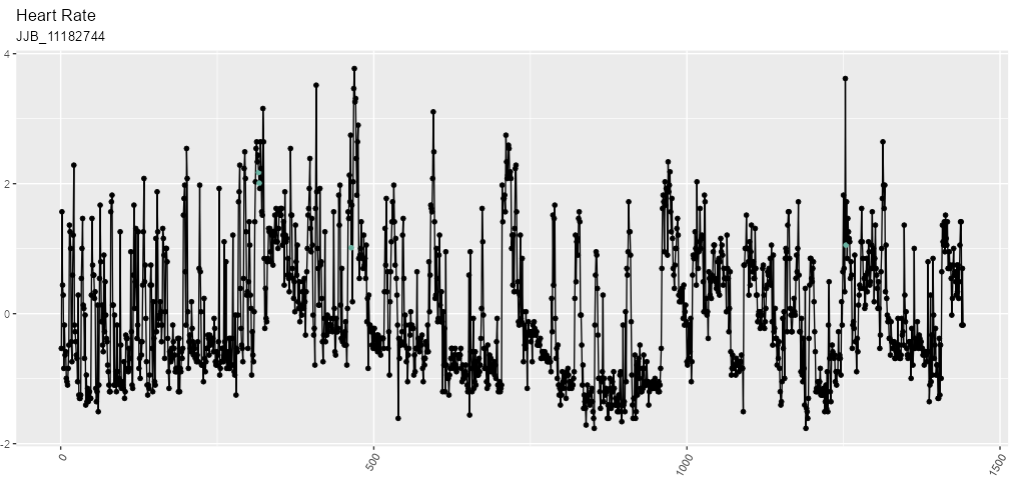
\includegraphics[scale=0.70]{./img/Heart-Rate-JJB.png}
    \caption{Valores de Frecuencia Cardíaca del paciente \textit{JJB\_11182744}}
    \label{fig:fc-JJB}
\end{figure}

\begin{figure}[H]
    \centering
    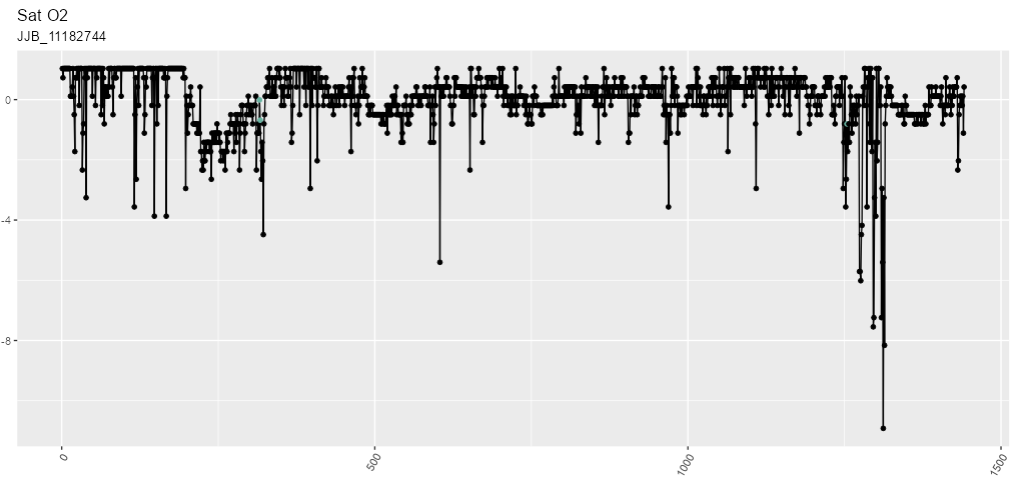
\includegraphics[scale=0.70]{./img/SatO2-JJB.png}
    \caption{Valores de Saturación de O$_2$ del paciente \textit{JJB\_11182744}}
    \label{fig:satO2-JJB}
\end{figure}

A la hora de trabajar con variables temporales se ha de tener en cuenta que los datos temporales pueden ser de dos tipos: \textit{Discretos} o \textit{Continuos}. Los datos discretos son aquellos que se recogen en intervalos de tiempo, por ejemplo, el número de pacientes que llegan a un hospital cada hora. Los datos continuos son aquellos que se recogen de forma continua, por ejemplo, en nuestro caso la saturación y frecuencia cardíaca de un paciente cada minuto.

Para terminar esta Sección \ref{sec:tiposdevariables} una última cuestión a valorar son las variables cualitativas y cuantitativas que se han recopilado. Las variables cualitativas son aquellas que describen una cualidad del paciente, por ejemplo, el sexo o la edad gestacional. Las variables cuantitativas son aquellas que describen una cantidad del paciente, por ejemplo, la frecuencia cardíaca o la saturación de oxígeno.

En la siguiente Tabla \ref{tabla:cuali_cuanti} se muestra la división entre variables cualitativas y cuantitivas recopiladas en el estudio y dentro del \textit{scope}.

\begin{table}[H]
    \centering
        \begin{tabular}{| m{5cm} | m{1.75cm} | m{7cm} |}
            \hline Tipo de Variable & Cantidad & Nombres  \\ \hline
            Cuantitativas & 15 & Edad, Peso, Edad Gestacional (EG), Horas de Ingreso tras inicio OAF, PCT (Procalcitonina en la sangre), PCR (Prueba de Proteína C relativa), Leucocitos, Nautrófilos, Linfocitos, Frecuencia Respiratoria (0 - 8 h), Frecuencia Respiratoria (8 - 16 h),
            Frecuencia Respiratoria (16 - 24 h),
            Flujo O$_2$ (0 - 8 h),
            Flujo O$_2$ (8 - 16 h),
            Flujo O$_2$ (16 - 24 h). \\ \hline
            Cualitativas & 27 & Sexo, Palivizumab, Lactancia Materna (LM), Dermatitis, Alergias, Tabaco, Enfermedad Base, Radiografía, Analítica, Suero, Etiología, Prematuridad, Alimentación, Sonda Nasogástrica, Gafas Nasales al Ingreso, OAF, OAF al ingreso, OAF tras ingreso, UCIP, Deterioro, Pausas de Apnea, Score Cruces Ingreso, SAPI (0 - 8 h),
            SAPI (8 - 16 h), 
            SAPI (16 - 24 h), Score Wood-Downes Ingreso y Score Wood-Downes 24 h. \\ \hline
            Otras & 2 & Notas e Identificador Paciente. \\ \hline
        \end{tabular}
    \caption{Variables Cualitativas y Cuantitativas Dentro del \textit{Scope}}\label{tabla:cuali_cuanti}
\end{table}

\subsection{Preprocesamiento de los Datos}

En este apartado se describirá el procesamiento de los datos realizado para el presente estudio.

\subsubsection{Limpieza de Datos}\label{sec:limpieza_datos}

En primer lugar se ha realizado una limpieza de datos. Esta limpieza de datos ha consistido en varios pasos: 

\begin{enumerate}
    \item \textbf{Validación de Archivos:} Contrastar que los diferentes archivos de datos no contienen datos duplicados o incoherencias.
    \item \textbf{Cálculo de Medias:} Calcular de manera automatizada las medias de \textit{Frecuencia Respiratoria} y \textit{Saturación de Oxígeno} cada hora. Estas medias han sido facilitadas en el Archivo de Datos de Pacientes pero por rigor se han vuelto a calcular para cada paciente. Ya que además que en la Carpeta de Datos de Monitorización se guardan los datos brutos con los que los médicos han calculado estas medias. Además de estas $2$ medias horarias, se han hecho dos trasformaciones en los datos de \textit{Frecuencia Cardiaca} que se explicarán más tarde. (\textit{Frecuencia Cardiaca Escalada} y \textit{Frecuencia Cardiaca por Cuantiles})
    \item \textbf{Datos Faltantes:} Determinar que pacientes y variables tienen un alto número de datos faltantes y eliminarlos del estudio.
    \item \textbf{Variables No Relevantes:} Eliminar variables que no aportan información relevante para el estudio.
\end{enumerate}

 \paragraph{Validación de Archivos}

Por parte del hospital se han recopilado 2 archivos de datos diferentes. Estos archivos de datos son:

\begin{itemize}
    \item \textbf{Archivo de Datos de Pacientes:} Este archivo contiene información descriptiva de los pacientes pediátricos. En este archivo se encuentran las variables contenidas en la Tabla \ref{tabla:cuali_cuanti}. Este archivo contiene 47 variables y 79 pacientes.
    \item \textbf{Carpeta de Datos de Monitorización:} En esta carpeta se almacena un archivo por cada paciente. Cada archivo contiene información temporal de los pacientes pediátricos. En este archivo se encuentran las variables \textit{Series Temporales} en la Tabla \ref{tabla:variables_estudio}. Por cada archivo se tienen 2 variables temporales (Saturación de O$_2$ y Frecuencia Cardiaca), cada variable presenta 1441 datos por paciente.
\end{itemize}

La Carpeta de Datos de Monitorización contiene 79 archivos de datos y el Archivo de Datos de Pacientes contiene 79 pacientes. Por lo tanto, se ha de contrastar que los datos de los pacientes contenidos en el Archivo de Datos de Pacientes estén contenidos en la Carpeta de Datos de Monitorización o si existen pacientes duplicados.

La cabecera de la Carpeta de Datos de Monitorización es la siguiente:
\begin{figure}[H]
    \centering
    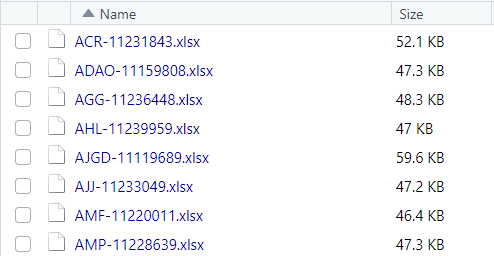
\includegraphics[scale=0.70]{./img/Carpeta-Monitor.png}
    \caption{Cabecera de la Carpeta de Datos de Monitorización}
    \label{fig:cabecera_monitorizacion}
\end{figure}

Y las primeras columnas del Archivo de Datos de Pacientes son las siguientes:
\begin{figure}[H]
    \centering
    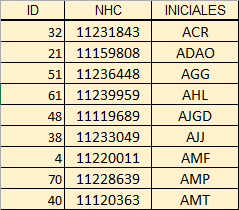
\includegraphics[scale=1.0]{./img/Archivo-Monitor.png}
    \caption{Cabecera de la Carpeta de Datos de Monitorización}
    \label{fig:cabecera_monitorizacion}
\end{figure}

Este contraste se ha automatizado de manera que para futuros estudios se pueda realizar de manera rápida y eficiente. El resultado de este contraste ha sido que los datos de los pacientes contenidos en el Archivo de Datos de Pacientes están contenidos en la Carpeta de Datos de Monitorización. Existían algunas desviaciones en los nombres pero fuero corregidas. Por lo tanto, no existen pacientes duplicados y se puede continuar con el estudio.

\paragraph{Cálculo de Medias}

En el Archivo de Datos de Pacientes venían calculadas las medias de \textit{Frecuencia Respiratoria} y \textit{Flujo de Oxígeno} cada hora. Estas medias han sido re-calculadas de manera automatizada para cada paciente y se han añadido al Archivo de Datos de Pacientes. Además de estas 2 medias se han hecho dos trasformaciones en los datos de \textit{Frecuencia Cardiaca} que se explicarán más tarde y se han calculado sus respectivas medias por hora. 

Se han calculado dos tipos de medias: 

\begin{itemize}
    \item \textbf{Medias No Nulas:} Se han calculado las medias de aquellos intervalos de hora dentro de las 24 h que no presentaban valores faltantes.
    \item \textbf{Medias Nulas:} Se han calculado las medias de aquellos intervalos de hora dentro de las 24 h sin importar si había momentos de valores valores faltantes dentro del intervalo hora.
\end{itemize}

Estos valores se han calculado para todos los pacientes, como modo de ejemplo el resultado para el paciente \textit{JJB\_11182744} ha sido el siguiente mostrado en la Tabla \ref{tabla:medias-JJB}:

% Se comienza una página nueva sin formato (sin número de página y sin encabezado/pie de página):
\newpage
\thispagestyle{empty}

% Se modifica la geometría (los márgenes) de la página y se coloca en formato horizontal:
\newgeometry{top=10mm, bottom=10mm, left=12mm, right=12mm}
\begin{landscape}

    \begin{table}[!ht]
        \centering
        \begin{tabular}{|l|l|l|l|l|l|l|l|l|l|l|l|}
        \hline
            hour & n & Missing\_FC & Missing\_SO2 & Mean\_FC & Mean\_SO2 & Mean\_Q & Mean\_SC & Mean\_FC\_NA & Mean\_SO2\_NA & Mean\_Q\_NA & Mean\_SC\_NA \\ \hline
            18 & 43 & 0 & 0 & 140,4186047 & 98,23255814 & 0,552067823 & -0,205230874 & 140,4186047 & 98,23255814 & 0,552067823 & -0,205230874 \\ \hline
            19 & 60 & 0 & 0 & 137,4666667 & 99,1 & 0,500688619 & -0,356544211 & 137,4666667 & 99,1 & 0,500688619 & -0,356544211 \\ \hline
            20 & 60 & 0 & 0 & 143,0166667 & 98,46666667 & 0,613802318 & -0,07205686 & 143,0166667 & 98,46666667 & 0,613802318 & -0,07205686 \\ \hline
            21 & 60 & 0 & 0 & 141,7 & 97,13333333 & 0,567600299 & -0,139547853 & 141,7 & 97,13333333 & 0,567600299 & -0,139547853 \\ \hline
            22 & 60 & 0 & 0 & 135,3666667 & 92,11666667 & 0,479248047 & -0,464188074 & 135,3666667 & 92,11666667 & 0,479248047 & -0,464188074 \\ \hline
            23 & 60 & 2 & 2 & ~ & ~ & ~ & ~ & 164,3448276 & 95,12068966 & 0,867006799 & 1,021202963 \\ \hline
            00 & 60 & 0 & 0 & 162,0666667 & 98,5 & 0,918496135 & 0,904426753 & 162,0666667 & 98,5 & 0,918496135 & 0,904426753 \\ \hline
            01 & 60 & 0 & 0 & 150,9833333 & 97,13333333 & 0,729509118 & 0,336306366 & 150,9833333 & 97,13333333 & 0,729509118 & 0,336306366 \\ \hline
            02 & 60 & 1 & 0 & ~ & 95,98333333 & ~ & ~ & 155,559322 & 95,98333333 & 0,762103523 & 0,570866889 \\ \hline
            03 & 60 & 0 & 0 & 142,3166667 & 96,01666667 & 0,606131522 & -0,107938147 & 142,3166667 & 96,01666667 & 0,606131522 & -0,107938147 \\ \hline
            04 & 60 & 0 & 0 & 142,2166667 & 96,86666667 & 0,569912026 & -0,113064045 & 142,2166667 & 96,86666667 & 0,569912026 & -0,113064045 \\ \hline
            05 & 60 & 0 & 0 & 130,6166667 & 97,8 & 0,37096502 & -0,70766824 & 130,6166667 & 97,8 & 0,37096502 & -0,70766824 \\ \hline
            06 & 60 & 0 & 0 & 155,8166667 & 96,4 & 0,762258703 & 0,584058113 & 155,8166667 & 96,4 & 0,762258703 & 0,584058113 \\ \hline
            07 & 60 & 0 & 0 & 132,55 & 96,73333333 & 0,405018753 & -0,608567541 & 132,55 & 96,73333333 & 0,405018753 & -0,608567541 \\ \hline
            08 & 60 & 0 & 0 & 129,4833333 & 97,06666667 & 0,344631214 & -0,765761753 & 129,4833333 & 97,06666667 & 0,344631214 & -0,765761753 \\ \hline
            09 & 60 & 0 & 0 & 127,8166667 & 97,18333333 & 0,312055141 & -0,85119339 & 127,8166667 & 97,18333333 & 0,312055141 & -0,85119339 \\ \hline
            10 & 60 & 0 & 0 & 151,2166667 & 96,43333333 & 0,703296936 & 0,348266795 & 151,2166667 & 96,43333333 & 0,703296936 & 0,348266795 \\ \hline
            11 & 60 & 0 & 0 & 156,55 & 97,41666667 & 0,87619425 & 0,621648034 & 156,55 & 97,41666667 & 0,87619425 & 0,621648034 \\ \hline
            12 & 60 & 0 & 0 & 145,95 & 98,1 & 0,685284072 & 0,078302822 & 145,95 & 98,1 & 0,685284072 & 0,078302822 \\ \hline
            13 & 60 & 0 & 0 & 146,4166667 & 98,13333333 & 0,704465169 & 0,10222368 & 146,4166667 & 98,13333333 & 0,704465169 & 0,10222368 \\ \hline
            14 & 60 & 0 & 0 & 129,9333333 & 97,08333333 & 0,372386073 & -0,742695211 & 129,9333333 & 97,08333333 & 0,372386073 & -0,742695211 \\ \hline
            15 & 60 & 1 & 1 & ~ & ~ & ~ & ~ & 155,220339 & 92,6779661 & 0,833584194 & 0,553490963 \\ \hline
            16 & 60 & 0 & 0 & 143,6333333 & 93,95 & 0,628285376 & -0,040447154 & 143,6333333 & 93,95 & 0,628285376 & -0,040447154 \\ \hline
            17 & 60 & 0 & 0 & 141,8666667 & 96,01666667 & 0,596238571 & -0,131004689 & 141,8666667 & 96,01666667 & 0,596238571 & -0,131004689 \\ \hline
            18\_1 & 18 & 0 & 0 & 156,1111111 & 96,05555556 & 0,890367072 & 0,599151036 & 156,1111111 & 96,05555556 & 0,890367072 & 0,599151036 \\ \hline
        \end{tabular}
        \caption{Medias Nulas y No Nulas de \textit{Frecuencia Cardíaca}, \textit{Saturación de O$_2$}, \textit{Cuantiles Cardíacos} y \textit{Frecuencia Cardíaca Escalada}  por hora para el paciente \textit{JJB\_11182744}}\label{tabla:medias-JJB}
    \end{table}

% Se devuelve el formato y la geometría de la página a sus valores originales:
\end{landscape}
\restoregeometry 

\paragraph{Datos Faltantes}

Se ha realizado un estudio de los datos faltantes. Este estudio ha consistido en determinar que pacientes y que variables tenían un alto número de datos faltantes y eliminarlos del estudio. 

\subparagraph*{Variables con Datos Faltantes} 

En la siguiente Figura~\ref{fig:missing-descriptive} se muestra la distribución de datos faltantes de las variables referenciadas en la Tabla \ref{tabla:cuali_cuanti}. 
 
\begin{figure}[H]
    \centering
    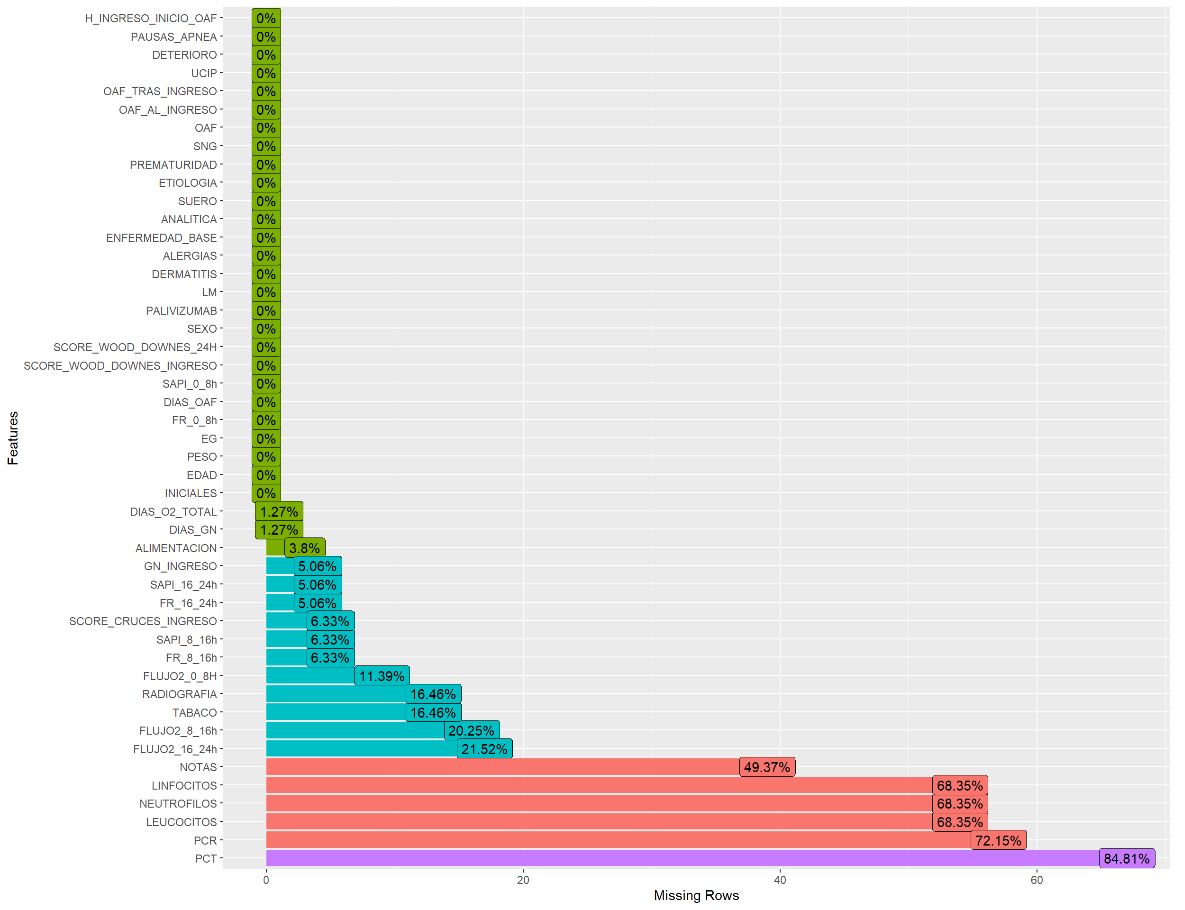
\includegraphics[scale = 0.70]{./img/missig-data-descriptive.png}
    \caption{Datos Faltantes en el Archivo de Datos de Pacientes}
    \label{fig:missing-descriptive}
\end{figure}

Por tro lado se ha estudiado que variables suelen faltar juntas. En la siguiente Imagen \ref{fig:missing-descriptive-cross} se muestra la distribución de datos faltantes cruzados de las 6 variables con mayor número de datos faltantes de la anterior Figura \ref{fig:missing-descriptive}.

\begin{figure}[H]
    \centering
    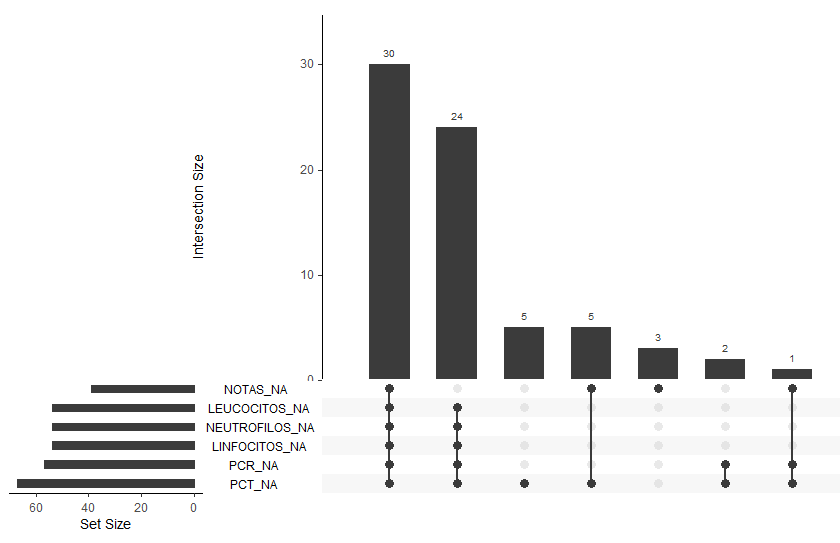
\includegraphics[scale = 0.70]{./img/missig-data-descriptive-cross.png}
    \caption{Datos Faltantes Cruzados de las 6 variables con Mayor Porcentaje de Datos Faltantes en el Archivo de Datos de Pacientes}
    \label{fig:missing-descriptive-cross}
\end{figure}

Según la Figura \ref{fig:missing-descriptive-cross} los \textit{Neutrofilos}, \textit{Linfocitos} y \textit{Leucocitos} se muestran faltantes siempre juntos, si falta uno faltan todos. Esto tiene sentido ya que los tres se obtienen si al paciente se le ha realizado una analítica. Por el contrario si solo contamos con los pacientes a los que se les ha realizado una analítica no hay faltantes de estas tres variables como se puede ver en la Figura \ref{fig:missing-descriptive-cross-analitica}. Es decir de manera sencilla, los datos faltantes de estas tres variables se deben a que no se le ha realizado una analítica al paciente.

\begin{figure}[H]
    \centering
    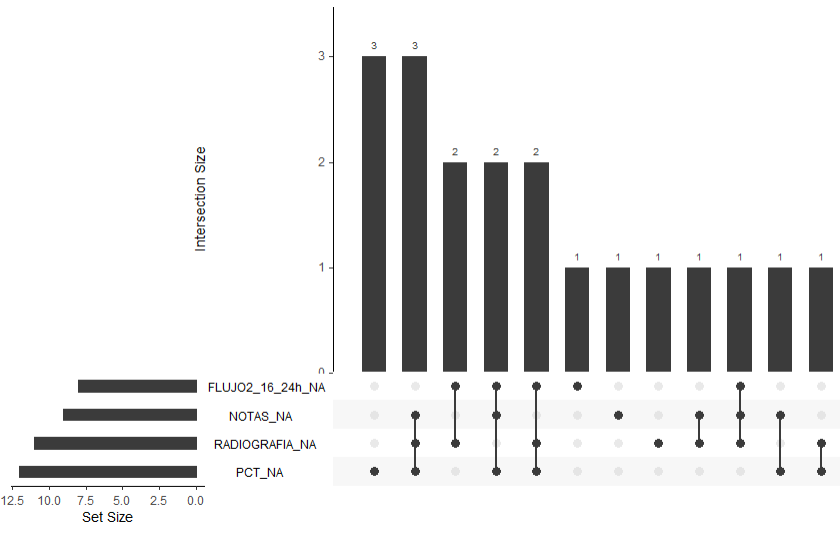
\includegraphics[scale = 0.70]{./img/missig-data-descriptive-cross-anal.png}
    \caption{Datos Faltantes Cruzados de las 4 variables con Mayor Porcentaje de Datos Faltantes en el Archivo de Datos de Pacientes si se le Ha Realizado una Analítica al Paciente}
    \label{fig:missing-descriptive-cross-analitica}
\end{figure}
\newpage




\subparagraph*{Pacientes con Datos Faltantes} 

Cuando se habla de pacientes con datos faltantes se hace referencia a aquellos pacientes que tienen datos faltantes en las variables \textit{Series Temporales} de la Tabla \ref{tabla:variables_estudio}. 

A cada paciente se le monitoriza durante las primeras 24 horas de su ingreso. En algunos casos, pueden ocurrir eventos que interrumpan la monitorización continua. Por ejemplo, si un paciente es trasladado a la Unidad de Cuidados Intensivos Pediátricos (UCIP), si es necesario realizarle alguna prueba o llevar a cabo tareas de higiene personal, se le desconecta de la monitorización. 

En la Figuras \ref{fig:fc-HGSDA} y \ref{fig:satO2-HGSDA} se muestran las \textit{Series Temporales} de \textit{Frecuencia Cardiaca} y \textit{Saturación de O$_2$} de el paciente \textit{HGSDA\_11233118} respectivamente. En estas se pueden observar como en ciertos momentos la monitorización se pausa y se registran valores faltantes en ciertos intervalos. 
\begin{figure}[H]
    \centering
    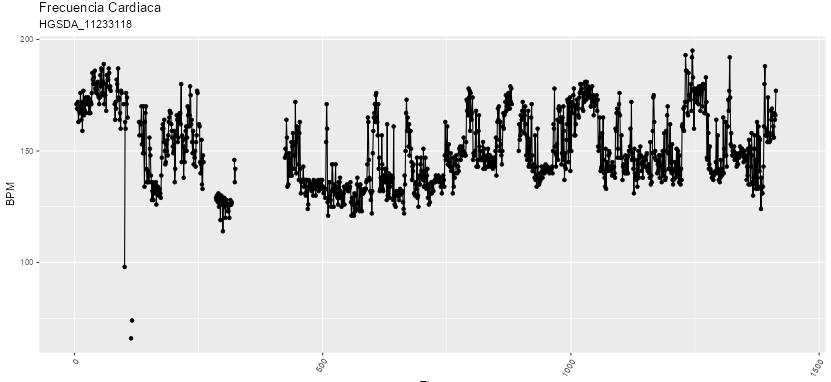
\includegraphics[scale=0.85]{./img/Heart-Rate-HGSDA.png}
    \caption{Valores de Frecuencia Cardíaca del paciente \textit{HGSDA\_11233118}}
    \label{fig:fc-HGSDA}
\end{figure}

\begin{figure}[H]
    \centering
    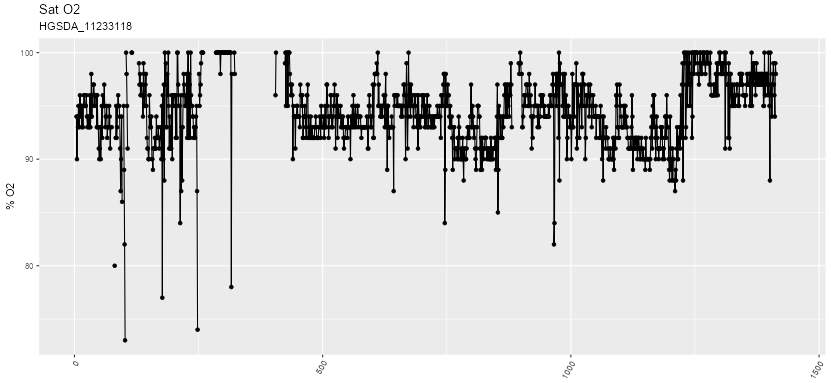
\includegraphics[scale=0.85]{./img/SatO2-HGSDA.png}
    \caption{Valores de Saturación de O$_2$ del paciente \textit{HGSDA\_11233118}}
    \label{fig:satO2-HGSDA}
\end{figure}


En la siguientes Figuras \ref{fig:missing-FC} y \ref{fig:missing-SatO2} se muestra la distribución y porcentaje de datos faltantes en las \textit{Series Temporales} de los 79 pacientes estudiados. La primera imagen hace referencia a la \textit{Frecuencia Cardiaca} y la segunda a la \textit{Saturación de O$_2$}.

% Se comienza una página nueva sin formato (sin número de página y sin encabezado/pie de página):
\newpage
\thispagestyle{empty}

% Se modifica la geometría (los márgenes) de la página y se coloca en formato horizontal:
\newgeometry{top=10mm, bottom=10mm, left=12mm, right=12mm}
\begin{landscape}

    \begin{figure}[H]
        \centering
        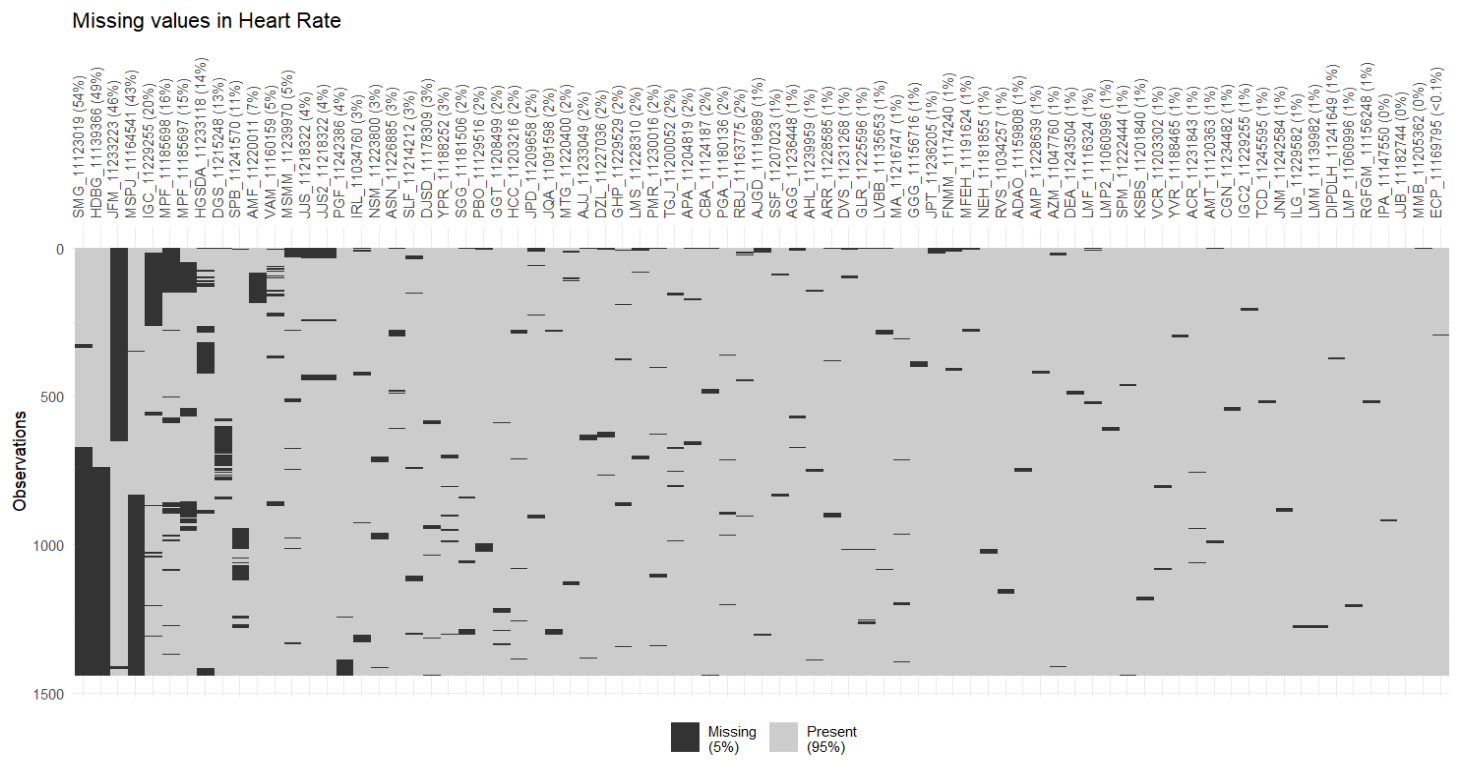
\includegraphics[scale = 0.9]{./img/missing-data-HR.png}
        \caption{Datos Faltantes en la \textit{Frecuencia Cardiaca} de los 79 pacientes pediátricos}
        \label{fig:missing-FC}
    \end{figure}
    
% Se devuelve el formato y la geometría de la página a sus valores originales:
\end{landscape}
\restoregeometry 

\newpage
\thispagestyle{empty}

% Se modifica la geometría (los márgenes) de la página y se coloca en formato horizontal:
\newgeometry{top=10mm, bottom=10mm, left=12mm, right=12mm}
\begin{landscape}

    \begin{figure}[H]
        \centering
        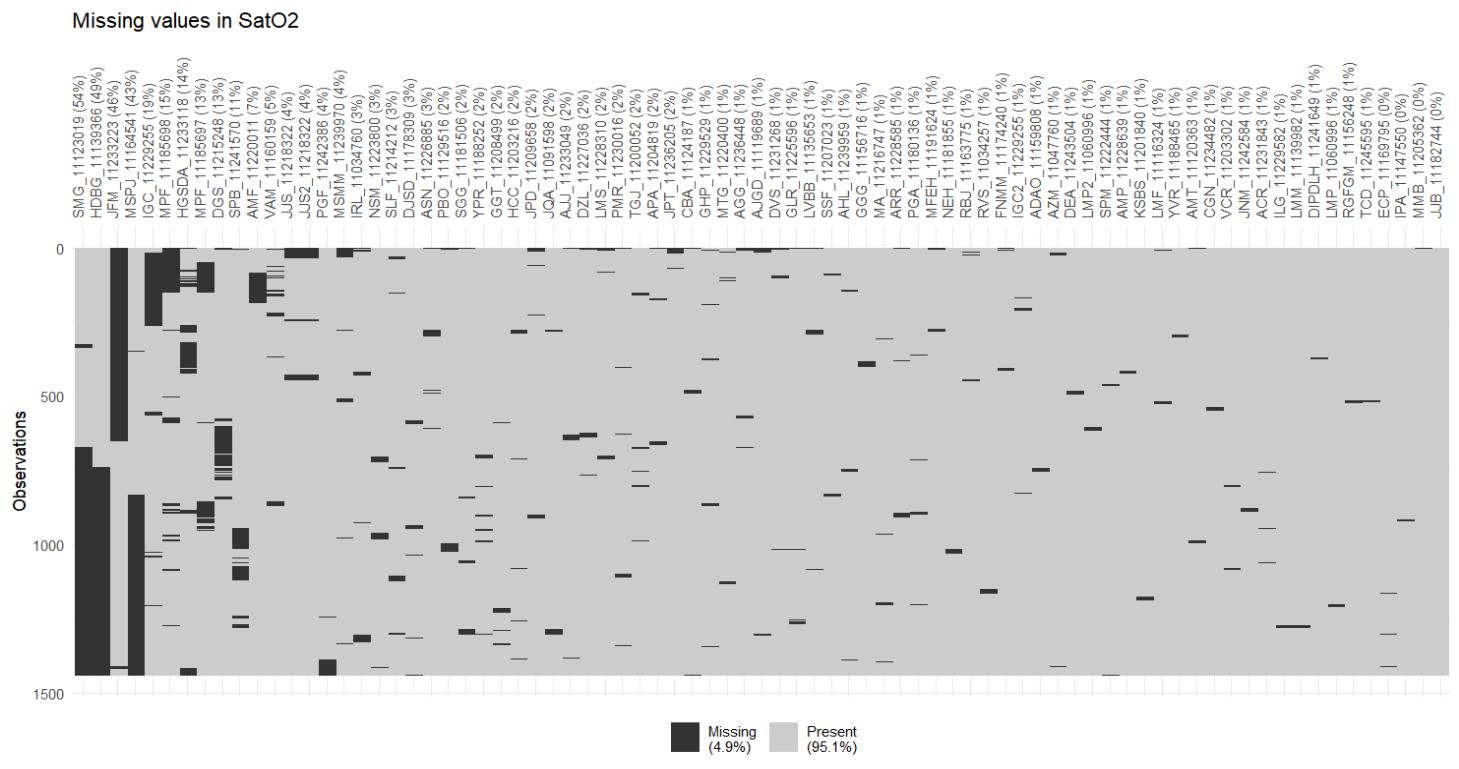
\includegraphics[scale = 0.9]{./img/missing-data-SatO2.png}
        \caption{Datos Faltantes en la \textit{Saturación de O$_2$} de los 79 pacientes pediátricos}
        \label{fig:missing-SatO2}
    \end{figure}
    
% Se devuelve el formato y la geometría de la página a sus valores originales:
\end{landscape}
\restoregeometry 

 A la hora de determinar los pacientes que van a ser incluidos en el estudio se va a tener en cuenta la variable \textit{Deterioro}. Esta variable indica si el paciente ha sufrido un deterioro durante las primeras 24 h de ingreso. Se considera \textit{Deterioro} si el paciente ha sido trasladado a la UCIP o ha recibido Oxigenación de Alto Flujo. 

 Estudiando los datos se ve como todos los pacientes que han sido trasladados a la UCIP han tenido previamente una intervención en la que se les ha aplicado Oxigenación de Alto Flujo pero no a todos a los que se les ha aplicado Oxigenación de Alto Flujo han sido trasladados a la UCIP. De esta forma los pacientes que muestren \textit{Deterioro} serán los mismos a los que se les ha aplicado OAF. Esto se puede ver en el diagrama de Venn en la Figura \ref{fig:venn-OAF-UCIP}.

\begin{figure}[H]
    \centering
    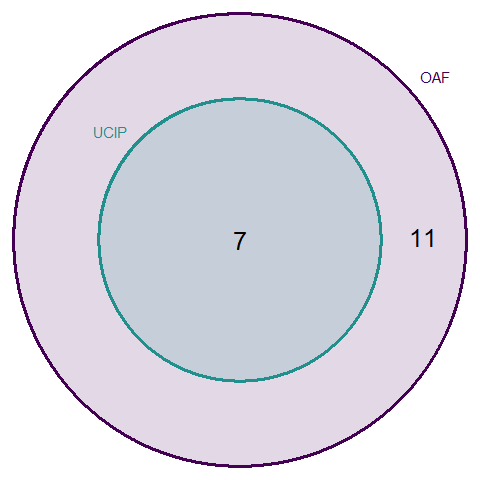
\includegraphics[scale = 1.50]{./img/venn-diagram-OAF-UCIP.png}
    \caption{Diagrama de Venn de los pacientes que han sido trasladados a la UCIP 7 y los que han recibido OAF $11 + 7 = 18$}
    \label{fig:venn-OAF-UCIP}
\end{figure}


Se utilizará la variable \textit{Deterioro} como indicadora de que el paciente ha sufrido OAF o ha sido trasladado a la UCIP. Según el Diagrama de Venn de la Figura \ref{fig:venn-OAF-UCIP} se puede ver como todos los pacientes que han sido trasladados a la UCIP han tenido previamente una intervención en la que se les ha aplicado Oxigenación de Alto Flujo pero no a todos a los que se les ha aplicado Oxigenación de Alto Flujo han sido trasladados a la UCIP. De esta forma los pacientes que muestren \textit{Deterioro} serán los mismos a los que se les ha aplicado OAF.


A la hora de eliminar pacientes será interesante ver cómo afecta también a la proporción de pacientes que han sufrido \textit{Deterioro} y los que no. En la siguiente Tabla \ref{tabla:ratio-deterioro} se muestra la cantidad de pacientes que presentan \textit{Deterioro}, los que no y el ratio entre \textit{Deterioro} y no \textit{Deterioro} del conjunto de pacientes totales.

\begin{table}[H]
    \centering
    \begin{tabular}{|m{2cm}|m{2.25cm}|m{2cm}|m{2cm}|}
    \hline
        Pacientes Totales & No Deterioro & Deterioro & Ratio \\ \hline
        79 & 61 & 18 & 0.295082 \\ \hline
    \end{tabular}
    \caption{Pacientes Totales, con Deterioro, sin Deterioro y Ratio entre Deterioro y No Deterioro}
        \label{tabla:ratio-deterioro}
\end{table}

\newpage

Se van a plantear dos metodologías para establecer la exclusión de pacientes en el estudio en función de las variables \textit{Series Temporales} de \textit{Frecuencia Cardiaca} y \textit{Saturación de O$_2$}. El objetivo es ver cómo varían la cantidad de pacientes incluidos en el estudio en ambos casos. Un paciente será incluido en el estudio si en las primeras horas establecidas su porcentaje de valores faltantes está por debajo de un \textit{threshold} establecido previamente. A continuación se muestran los dos métodos propuestos: 

\begin{itemize}
    \item \textbf{Método 1:} Se va a ir aumentando progresivamente el \textit{threshold} de valores faltantes desde el $5 \%$ hasta el $20 \%$ en intervalos de $2.5 \%$.  Es decir se va a estudiar si existen más pacientes que cumplen el criterio de admisión en las primeras $24$ horas cambiando el \textit{threshold}. Este método se puede ver en la Figura \ref{fig:metodo1}.
    \item \textbf{Método 2:} Se va a establecer un \textit{threshold} en el $5 \%$ de valores faltantes. Una vez establecido dicho \textit{threshold} se va a ir aumentando el tiempo de \textit{scope} del estudio. Es decir, en vez de plantear estudiar las $24$ primeras horas como se ha planteado en el \textit{Método 1}, se va a estudiar si centrándose en un intervalo menor de estudio existen más pacientes que cumplen este criterio de admisión. Se va a ir aumentando el intervalo de estudio desde las $8$ primeras h en intervalos de $30$ minutos hasta las primeras $15$ horas. Es decir se va a estudiar si existen más pacientes que cumplen el criterio de admisión en las primeras $8$ horas, en las primeras $8.5$ horas, en las primeras $9$ horas, etc. hasta llegar a las $15$ primeras horas. Este método se puede ver en la Figura \ref{fig:metodo2}.
\end{itemize}

\begin{figure}[H]
    \centering
    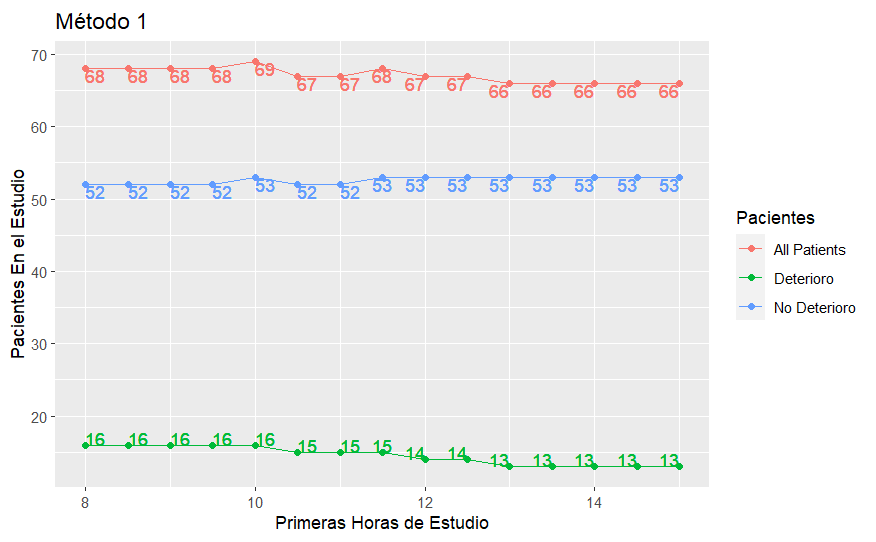
\includegraphics[scale = 1]{./img/metodo1.png}
    \caption{Método 1 de Exclusión de Pacientes}
    \label{fig:metodo1}
\end{figure}

\begin{figure}[H]
    \centering
    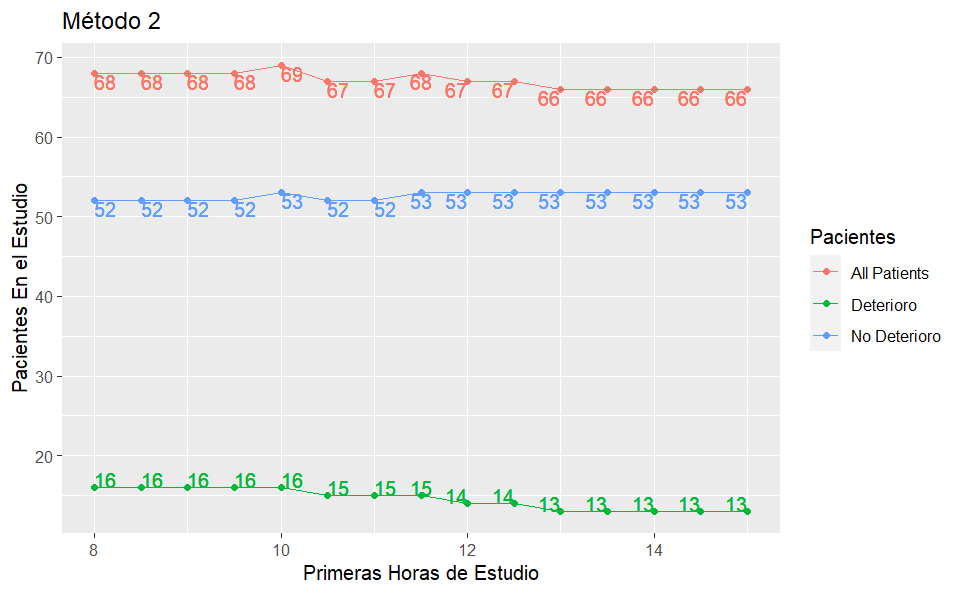
\includegraphics[scale = 1]{./img/metodo2.png}
    \caption{Método 2 de Exclusión de Pacientes}
    \label{fig:metodo2}
\end{figure}

Con los anteriores métodos se ha podido observar cómo realmente el hecho de ser más restrictivos con los datos faltantes no implica que se vayan a excluir muchos más pacientes, y el cambio del ratio $\frac{\textit{Pacientes con Deterioro}}{\textit{Pacientes No Deterioro}}$ es casi inapreciable. Por lo tanto, los datos faltantes se acumulan en un número concreto de pacientes a los que el seguimiento se les ha interrumpido en mayor medida.

En la situación más restrictiva del \textit{Método 1} de la Figura \ref{fig:metodo1} el ratio es de $ \frac{14}{54} \approx 0.26$ y en la menos restrictiva es de $ \frac{16}{59} \approx 0.272$. Cabe decir que la situación más restrictiva es aquella que en las primeras $24$ horas se pide que haya un menor porcentaje de valores faltantes, es decir la combinación de valores más a la izquierda en el eje $x$ de la Figura \ref{fig:metodo1}. Este método muestra un considerable aumento de la muestra de pacientes si se opta por la opción menos restrictiva respecto a la más restrictiva, se pasa de $68$ pacientes a $75$ aumentando en casi un $10 \%$ la muestra total. 

Por otro lado en la situación más restrictiva del \textit{Método 2} de la Figura~\ref{fig:metodo2} el ratio es de $ \frac{13}{53} \approx 0.245$ y en la situación menos restrictiva el ratio es de $ \frac{13}{53} \approx 0.245$. La variación total de pacientes a incluir en el estudio es de apenas un $3 \%$, se pasa de $68$ pacientes a excluir a $2$ en la situación más restrictiva, obteniendo un total de $66$ pacientes. Cabe aclarar que la situación más restrictiva según este método es aquella que considera más horas de monitorización manteniendo el \textit{threshold} en el $5 \%$ de valores faltantes, es decir la combinación de valores más alejada en el eje $x$ de la Figura \ref{fig:metodo2}.

Para no alterar los datos debido a una posterior imputación y debido a que la variación de los datos es algo importante en el estudio se optará por establecer el \textit{threshold} en el $5 \%$ de valores faltantes, haciendo referencia a la siguiente entrada bibliográfica: \cite{Scheffer2002}. 

Junto con este último criterio mencionado se van a hacer dos grupos de pacientes a la hora de hacer el estudio planteado por el presente Trabajo de Fin de Máster:

\begin{itemize}
    \item \textbf{Valid\_patients\_P1:} Serán aquellos que en las primeras 24 horas de monitorización tengan un porcentaje de valores faltantes por debajo del $5\%$. Estos pacientes serán aquellos que sigan el criterio más restrictivo del \textit{Método 1} de la Figura \ref{fig:metodo1}. 
    \begin{table}[H]
        \centering
        \begin{tabular}{|m{2cm}|m{2.25cm}|m{2cm}|m{2cm}|}
        \hline
            Pacientes Totales & No Deterioro & Deterioro & Ratio \\ \hline
            68 & 54 & 14 & 0.26 \\ \hline
        \end{tabular}
        \caption{Pacientes Totales, con Deterioro, sin Deterioro y Ratio entre Deterioro y No Deterioro seleccionados para el estudio según el \textit{Método 1}}\label{tabla:ratio-deterioro-P1}
    \end{table}
    \item \textbf{Valid\_patients\_P2:} Serán aquellos que en las primeras $8$ horas de monitorización tengan un porcentaje de valores faltantes por debajo del $5\%$. Estos pacientes serán aquellos que siguen el criterio más restrictivo del \textit{Método 2} de la Figura \ref{fig:metodo2}. Además, se excluirán aquellos pacientes que hayan presentado \textit{Deterioro} en las primeras 8 horas de monitorización. Esto será así, pues se pretende predecir en las primeras $8$ horas qué pacientes son los que van a presentar \textit{Deterioro} en las próximas horas.
    \begin{table}[H]
        \centering
        \begin{tabular}{|m{2cm}|m{2.25cm}|m{2cm}|m{2cm}|}
        \hline
            Pacientes Totales & No Deterioro & Deterioro & Ratio \\ \hline
            58 & 52 & 6 & 0.115 \\ \hline
        \end{tabular}
        \caption{Pacientes Totales, con Deterioro, sin Deterioro y Ratio entre Deterioro y No Deterioro seleccionados para el estudio según el \textit{Método 2} y exclusión de pacientes con \textit{Deterioro} en las primeras 8 horas de monitorización}
            \label{tabla:ratio-deterioro-P1}
    \end{table}
\end{itemize}

Se ha decidido pues que se van a realizar $2$ estudios:

\begin{itemize}
    \item \textbf{Estudio 1:} Se estudiarán a los pcientes pediátricos tomando como referencia las primeras $24$ horas de monitorización, se querrá así pues mantener la unidad \textit{día} en el estudio. Se ha visto que reduciendo el \textit{scope} según el \textit{Método 2} no se consigue un aumento de la muestra de pacientes significativa, y por otro lado reducir la restricción de pacientes con valores faltantes por encima del $5\%$ para aumentar la cantidad de pacientes en el estudio, no es recomendable según la referencia \cite{Scheffer2002}.
    \item \textbf{Estudio 2:} Se estudiarán a los pacientes pediátricos tomando como referencia las primeras $8$ horas de monitorización y excluyendo a aquellos pacientes que han presentado OAF en esas 8 primeras horas así como las variables que se registran más tarde de las $8$ primeras horas. Se ha decidido utilizar las primeras $8$ horas de monitorización ya que se pretende predecir en las primeras $8$ horas qué pacientes son los que van a presentar \textit{Deterioro} en las siguientes próximas horas.
\end{itemize}


\subsubsection{Imputación de Datos}\label{sec:imputacion-de-datos}

Una vez que se han decidido los pacientes que se van a incluir tanto en el \textit{Estudio 1} como en el \textit{Estudio 2} se ha de realizar una imputación de datos para permitir a los algoritmos de clasificación discreta poder trabajar con el total de los pacientes, no solo con aquellos que no muestran datos faltantes. 

La imputación de datos se hará en dos documentos diferentes:
\begin{itemize}
    \item \textbf{Archivo de Datos de Pacientes:} En este archivo se imputarán los datos faltantes de las variables \textit{Cuantitativas} y \textit{Cualitativas} de la Tabla~\ref{tabla:cuali_cuanti} mediante el método de la \textit{distancia de Gower}.
    \item \textbf{Carpeta de Datos de Monitorización:} En esta carpeta se imputarán los datos numéricos faltantes de las variables \textit{Series Temporales} que aparecen referenciadas en la Tabla~\ref{tabla:variables_estudio} mediante el método de \textit{k-Nearest Neighbor Imputation}.
\end{itemize}

Cada imputación se hará de una manera diferente. En el primer caso ya que es necesario imputar datos de variables cualitativas y cuantitativas se utilizará el método de \textit{Distancia de Gower}, Sección~\ref{sec:gower_distance} y en el segundo caso se utilizará el método de \textit{k-Nearest Neighbor Imputation}, Sección~\ref{sec:k_Nearest Neighbor_Imputation} ya que muestra mejores resultado a la hora de solo imputar solo variables numéricas.

En el caso de la Frecuencia Cardiaca se realizará una transformación a la cual más tarde se le imputarán datos y se utilizarán como parte del \textit{Estudio 2}. Se hablará de esta transformación más adelante en la Sección~\ref{sec:transformaciones-de-datos}. La imputación de datos se hará una vez realizada la transformación, es decir de \textit{Frecuencia Cardiaca} de cada paciente válido para el estudio en cuestión.

\paragraph{Distancia de Gower}\label{sec:gower_distance}

La \textit{distancia de Gower} puede utilizarse para medir la diferencia entre dos registros que pueden contener una combinación de datos lógicos, numéricos, categóricos o textuales. La distancia es siempre un número comprendido entre 0 (idéntico) y 1 (máxima diferencia). La \textit{distancia de Gower} se calcula como el promedio de las disimilitudes parciales entre individuos. Cuanto menor es el número, más similares son los individuos.

El coeficiente de disimilitud como lo define Gower en su artículo puede ser utilizado para medir la distancia entre dos puntos en un espacio multidimensional y puede ser calculado utilizando diferentes métodos; dependiendo del tipo de datos y del espacio en el que se encuentran los puntos. (~\cite{Gower1971}~)

La imputación de datos se realiza según el código programado que se muestra en la Sección:~\ref{sec:codigo-input-gower}. El código funciona de la siguiente forma: 
\begin{enumerate}
    \item Antes de nada es necesario seleccionar e introducir en la función los siguientes parámetros formales: 
    \begin{itemize}
        \item \texttt{dat}: El conjunto de datos que van a ser utilizados para la imputación (no deben tener datos faltantes). Es decir existe un subconjunto de datos del conjunto de datos total que se utiliza como base de imputación y es de dónde se calculan las distancias respecto al nuevo paciente al que se le quieren imputar datos.
        \item \texttt{new\_with\_null}: El paciente al que se le quieren imputar datos. Dicho paciente se introduce en la función con sus valores faltantes.
        \item \texttt{n\_primeros}: La cantidad $k$ de \textit{vecinos} que se van a tener en cuenta en relación con el paciente al que se le quieren imputar datos. En el caso de este estudio se ha establecido en 5 vecinos, es necesario que sea impar para que la mediana en los datos cualitativos de dos factores con dos opciones se decante por una, cuando hay más factores la situación se complica. 
    \end{itemize}
    \item En segundo lugar se calcula la distancia de Gower entre el paciente seleccionado y el resto de pacientes teniendo solo en cuenta las variables sin datos faltantes. La distancia se calcula entre los pacientes que tienen datos en las variables que se quieren imputar.
    \item Se separan las variables con datos faltantes en cualitativas y cuantitativas, y se seleccionan los $k$ pacientes más parecidos.
    \item Se calcula la media de los valores de las variables cuantitativas de los $k$ pacientes más parecidos y se imputan en el paciente seleccionado.
    \item Se calcula la mediana de los valores de las variables cualitativas de los $k$ pacientes más parecidos y se imputan en el paciente seleccionado.
\end{enumerate}

Es necesario cuando se tiene un conjunto de datos con mezcla de pacientes con valores faltantes hacer un preprocesamiento de los datos para la correcta imputación. Ese preprocesamiento consta de dos pasos: 
\begin{itemize}
    \item \textbf{Separar los pacientes con datos completos de los que no:} Se separan los pacientes con datos completos de los que no. Los pacientes con datos completos se utilizan para imputar a los pacientes don datos faltantes.
    \item \textbf{Imputar sucesivamente:} Se imputan sucesivamente los pacientes con datos faltantes. Es decir, se imputan los datos de un paciente con datos faltantes y se añade a la lista de pacientes con datos completos, separada de la utilizada para imputación. Se ha decidido que nunca se utilizará un paciente con datos imputados para imputar a otro paciente.
\end{itemize}

Los códigos programados que siguen la lógica anteriormente descrita y utilizados para la imputación por este método de la distancia de Gower se encuentran en la Sección~\ref{sec:codigo-input-gower-fun-preprocesamiento}.

El diagrama de flujo dónde se explica lo anteriormente descrito es el siguiente: 

\newpage
\thispagestyle{empty}

% Se modifica la geometría (los márgenes) de la página y se coloca en formato horizontal:
\newgeometry{top=10mm, bottom=10mm, left=12mm, right=12mm}
\begin{landscape}
    \begin{figure}[H]
        \centering
        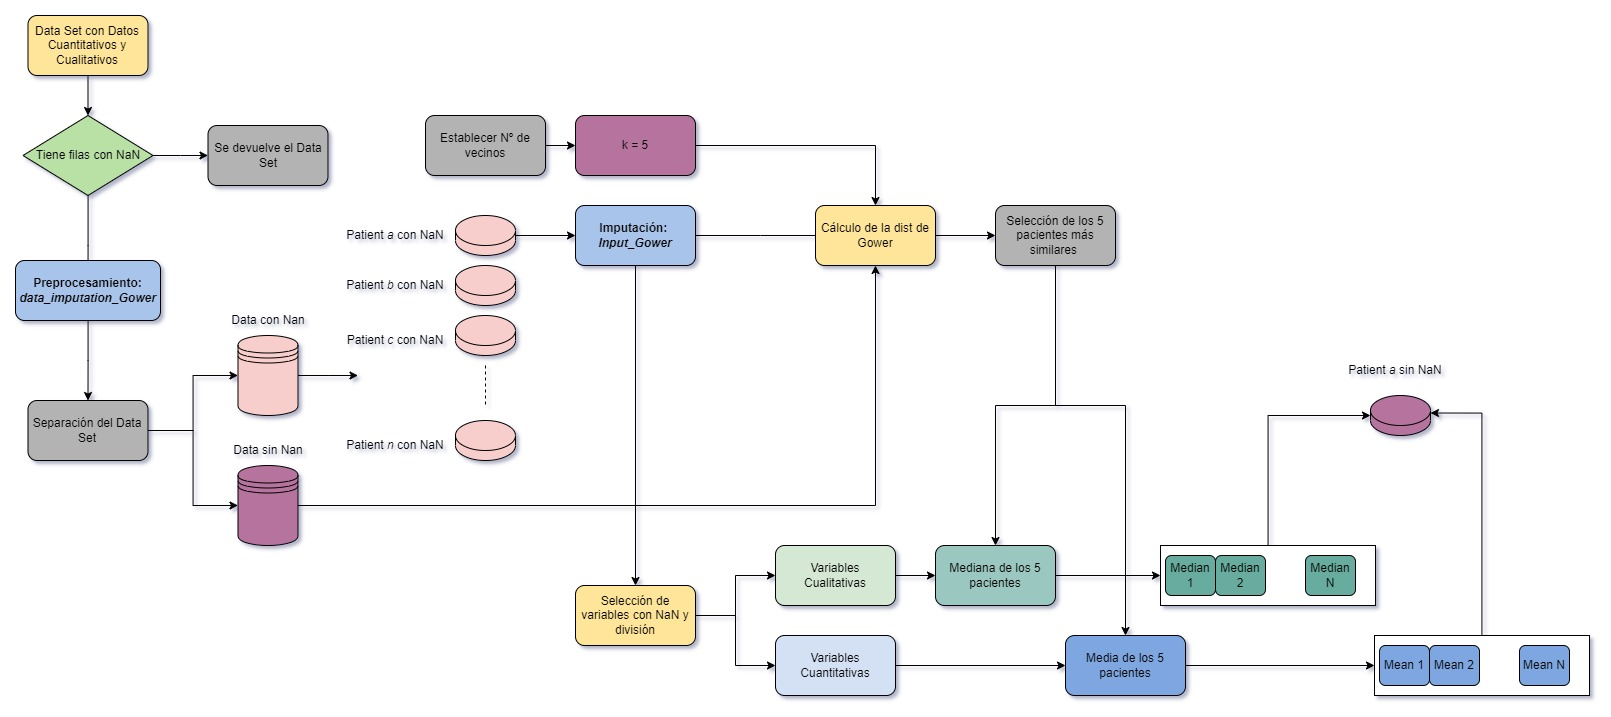
\includegraphics[scale = 0.5]{./img/gower-diagram.jpg}
        \caption{Diagrama de Flujo Imputación por el método de la distancia de Gower}
        \label{fig:gower-diagram}
    \end{figure}
% Se devuelve el formato y la geometría de la página a sus valores originales:
\end{landscape}
\restoregeometry 



\paragraph{k-Nearest Neighbor Imputation}\label{sec:k_Nearest Neighbor_Imputation}

El método de \textit{k-Nearest Neighbor Imputation} al igual que la distancia de Gower es un método de imputación de datos que se basa en la distancia entre los pacientes. Este método se fundamenta en la premisa de que los pacientes que son similares presentan valores parecidos en las variables que se desean imputar. En este caso se ha utilizado el paquete \texttt{DMwR2} de \texttt{R} para realizar la imputación.~(\cite{DMwR2}).

La imputación \textit{k-Nearest Neighbor Imputation} es un método utilizado para rellenar los valores que faltan en un conjunto de datos utilizando los valores de los $k$ vecinos más próximos. Este método es especialmente útil para variables numéricas, en las que los valores que faltan pueden sustituirse por la media de los $k$ vecinos más próximos.

La ventaja de este método respecto a la \textit{distancia de Gower} es que aparte de que ya viene construido el algoritmo de imputación en el paquete de Rstudio \textit{DMwR2}, es que solo se imputarán datos numéricos y para esta casuística es método más adecuado y programado orientado a este objetivo.

Un ejemplo que ilustra este enfoque de imputación se encuentra en el estudio titulado \textit{Missing Data Imputation for Geolocation-based Price Prediction Using KNN MCF Method} \cite{Sanjar2020}. En este trabajo, se empleó la técnica de imputación conocida como \textit{k-Nearest Neighbor Imputation}, lo cual permitió mejorar significativamente la precisión del modelo y evitar problemas de sobreajuste. El método propuesto alcanzó una precisión de predicción del $92.01$\%, con la asistencia del algoritmo de clasificación \textit{Random Forest}.

La función usada de imputación usará los $5$ vecinos más cercanos y el método de imputación es el de la media ponderada de los vecinos más cercanos \textit{weighAvg}. La función de imputación una vez que identifica los k vecinos más cercanos, calculan los pesos para cada uno de ellos en función de la distancia a la observación original que tiene el valor al faltante. Los vecinos más cercanos tienen mayor influencia a la hora de la imputación debido a sus mayores pesos. La media ponderada se utiliza como el valor imputado para el dato faltante en la observación original. La función usada para la imputación es la siguiente referenciada en el Código~\ref{cod:snipet-knn-impute}:

\begin{code}[H]
\begin{lstlisting}
    knnImputation(data, k = 5, scale = T, meth = "weighAvg",
    distData = NULL)
\end{lstlisting}
\caption{Código KNN Impute Función}
\label{cod:snipet-knn-impute}
\end{code}

Respecto a los valores imputados mediante este método serán los valores faltantes de las \textit{Series Temporales} referenciados en la Tabla~\ref{tabla:variables_estudio} y sus respectivas transformaciones sobre las que más tarde se hablará de ellas en la Sección~\ref{sec:transformaciones-de-datos}. 

A la hora de imputar datos cabe diferenciar entre los dos Estudios realizados. Cada estudio considera unos pacientes en un intervalo de tiempo diferente. Debido a esta casuística se ha decidido imputar los datos de los pacientes de cada estudio por separado. Es decir, se imputarán los datos de los pacientes del \textit{Estudio 1} por un lado y los del \textit{Estudio 2} por otro.

\subparagraph*{Diagrama de imputación de datos de \textit{Series Temporales} por el método de imputación \textit{k-Nearest Neighbor Imputation}}\label{sec:diagrama-imputacion-knn} \\

Cada paciente será estudiado de manera individualizada. Esto implica que los datos de monitorización de cada \textit{Series Temporal} en referencia a cada paciente se tienen que dividir en diferentes en franjas horarias para así realizar la imputación de datos. Estas franjas horarias dependerá del tipo de estudio. En el \textit{Estudio 1} las franjas horarias serán $40$ de $36$ minutos cada una lo que hace un total de $1440$ minutos que son justamente las $24$ horas de estudio, Figura~\ref{fig:knn-diagram-e1}. En el \textit{Estudio 2} las franjas horarias serán $20$ de $24$ minutos lo que hace un total de $480$ minutos que son justamente las $8$ horas de estudio, Figura~\ref{fig:knn-diagram-e2}.

Una vez que se han dividido los datos de cada paciente en franjas horarias se imputarán los datos de cada franja horaria por separado. Es decir, se imputarán los datos de la primera franja horaria de cada paciente en relación con las 5 más cercanas, después los de la segunda, etc, así hasta llegar a la última franja horaria de cada paciente. Es obvio que solo se imputarán datos de las franjas horarias que tengan datos faltantes y se utilizarán las $5$ franjas horarias más cercanas que tengan datos en el minuto que se quiera imputar.

\newpage
\thispagestyle{empty}
% Se modifica la geometría (los márgenes) de la página y se coloca en formato horizontal:
\newgeometry{top=10mm, bottom=10mm, left=12mm, right=12mm}
\begin{landscape}
    \begin{figure}[H]
        \centering
        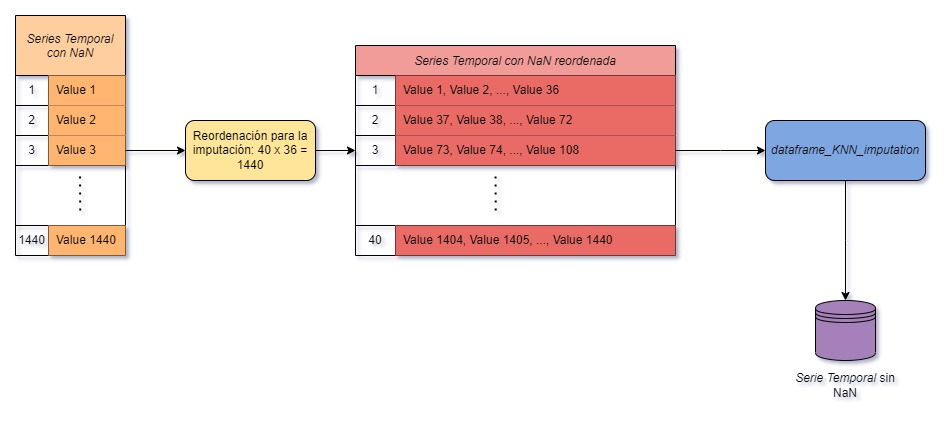
\includegraphics[scale = 0.5]{./img/knn-diagram-e1.jpg}
        \caption{Diagrama de Flujo Imputación por el método de \textit{k-Nearest Neighbor Imputation} según el \textit{Estudio 1}}
        \label{fig:knn-diagram-e1}
    \end{figure}
    \begin{figure}[H]
        \centering
        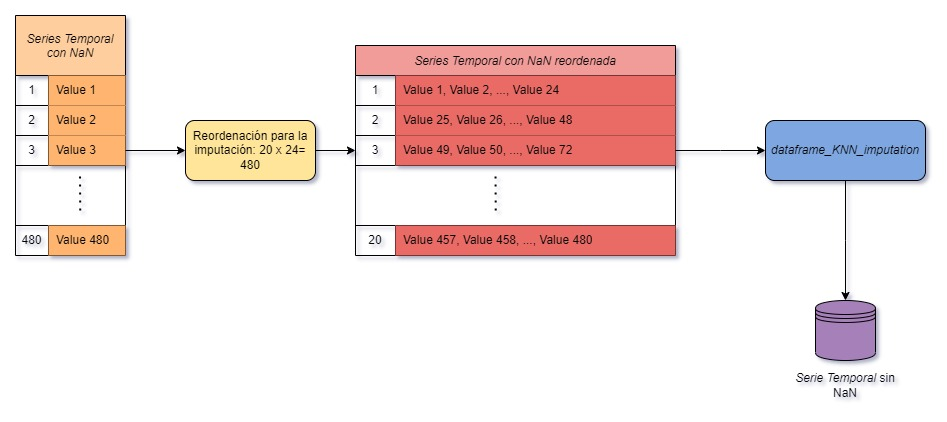
\includegraphics[scale = 0.5]{./img/knn-diagram-e2.jpg}
        \caption{Diagrama de Flujo Imputación por el método de \textit{k-Nearest Neighbor Imputation} según el \textit{Estudio 2}}
        \label{fig:knn-diagram-e2}
    \end{figure}
% Se devuelve el formato y la geometría de la página a sus valores originales:
\end{landscape}
\restoregeometry 

\subsubsection{Transformaciones de los Datos}\label{sec:transformaciones-de-datos}

En el presente \textit{Trabajo de Fin de Máster} se ha pretendido eliminar el componente \textit{EDAD} de los datos de monitorización de los pacientes pediátricos. Esto se ha hecho para que los algoritmos de clasificación discreta (\textit{Random Forest}) no se centren en la edad del paciente a la hora de predecir si el paciente va a presentar \textit{Deterioro} o no. Para eliminar este componente, se ha recurrido al estudio de Fenton et al. \cite{percentilesFenton2015}, el cual define rangos normales y percentiles para las frecuencias cardíacas y respiratorias en lactantes y niños, a partir de un estudio transversal de pacientes que acudieron a un servicio de urgencias pediátrico en un hospital australiano. Se utilizarán de dicho estudio los valores en referencia a la \textit{Frecuencia Cardiaca}. A continuación se muestran los valores de \textit{Frecuencia Cardiaca} en función de la \textit{Edad} en 

\newpage
\thispagestyle{empty}
% Se modifica la geometría (los márgenes) de la página y se coloca en formato horizontal:
\newgeometry{top=10mm, bottom=10mm, left=12mm, right=12mm}
\begin{landscape}
    \begin{table}[htbp]
        \centering
        \caption{Age-related percentiles}
        \label{tab:age_percentiles}
        \begin{tabular}{|l|l|l|l|l|l|l|l|l|l|l|l|}
            \toprule
            Age & Age\_0 & {Amount} & {1st} & {5th} & {10th} & {25th} & {50th} & {75th} & {90th} & {95th} & {99th} \\
            \midrule
            0--$<$3 months & months & 3365,00 & 109,00 & 119,00 & 123,00 & 132,00 & 142,00 & 154,00 & 165,00 & 171,00 & 181,00 \\
            3--$<$6 months & months & 4493,00 & 100,00 & 113,00 & 118,00 & 124,00 & 135,00 & 145,00 & 155,00 & 161,00 & 174,00 \\
            6--$<$9 months & months & 5927,00 & 100,00 & 110,00 & 115,00 & 121,00 & 131,00 & 141,00 & 151,00 & 159,00 & 172,00 \\
            10--$<$12 months & months & 6005,00 & 98,00 & 105,00 & 111,00 & 119,00 & 127,00 & 139,00 & 150,00 & 160,00 & 174,00 \\
            12--$<$18 months & months & 10,00 & 94,00 & 101,00 & 107,00 & 116,00 & 124,00 & 136,00 & 149,00 & 159,00 & 176,00 \\
            18--$<$24 months & months & 9370,00 & 90,00 & 99,00 & 103,00 & 112,00 & 120,00 & 132,00 & 145,00 & 154,00 & 172,00 \\
            2--$<$3 years & years & 15,00 & 85,00 & 96,00 & 99,00 & 107,00 & 117,00 & 126,00 & 138,00 & 146,00 & 162,00 \\
            3--$<$4 years & years & 11,00 & 80,00 & 89,00 & 94,00 & 102,00 & 111,00 & 121,00 & 131,00 & 138,00 & 152,00 \\
            4--$<$6 years & years & 15,00 & 74,00 & 82,00 & 88,00 & 96,00 & 105,00 & 117,00 & 126,00 & 133,00 & 146,00 \\
            6--$<$8 years & years & 9100,00 & 69,00 & 78,00 & 81,00 & 90,00 & 100,00 & 111,00 & 122,00 & 128,00 & 141,00 \\
            8--$<$12 years & years & 12,00 & 64,00 & 72,00 & 77,00 & 84,00 & 94,00 & 104,00 & 116,00 & 122,00 & 135,00 \\
            12--$<$15 years & years & 6054,00 & 59,00 & 64,00 & 69,00 & 77,00 & 86,00 & 97,00 & 106,00 & 113,00 & 127,00 \\
            15--$<$16 years & years & 1339,00 & 56,00 & 62,00 & 66,00 & 74,00 & 83,00 & 94,00 & 103,00 & 111,00 & 122,00 \\
            \bottomrule
        \end{tabular}
    \end{table}
\end{landscape}
\restoregeometry 

 







\newpage

\section{CAPÍTULO IV: METODOLOGÍA}\label{cap:methodology}

En este capítulo, se comenzará por discutir el diseño de la investigación para más tarde describir la metodología utilizada para conseguir cumplir los objetivos planteados en la Sección~\ref{sec:objectives}. 

Este capítulo estará en relación con el Capítulo~\ref{cap:resultsANDdiscussion} de manera que cada enfoque metodológico aportado en el presente capítulo mostrará sus resultados en el siguiente, de esta forma existirá una relación directa entre los apartados: *** 


\subsection{Diseño de Investigación}

Se ha utilizado un enfoque de investigación cuantitativa para examinar la progresión temporal de la bronquiolitis en pacientes pediátricos. De cara a alcanzar los objetivos planteados en la Sección~\ref{sec:objectives} se discutirá como la muestra limita el cumplimiento de algunos de los objetivos y frente a este límite se van a plantear diferentes alternativas. 

Como ya se ha introducido anteriormente se van a realizar $2$ estudios diferentes con distinto enfoque. A continuación se explicarán por qué se ha decidido realizar 2 estudios diferentes y se discutirán como se deben de replantear los objetivos plantados en la Sección~\ref{sec:objectives}.

Al tener 3 momentos de valoración, que son los que se muestran a continuación:

\begin{enumerate}
    \item $0$ horas $\leq$ Tiempo de Monitorización $<$ $8$ horas 
    \item $8$ horas $\leq$ Tiempo de Monitorización $<$ $16$ horas
    \item $16$ horas $\leq$ Tiempo de Monitorización $<$ $24$ horas
\end{enumerate}


Se ha plantado que se realicen valoraciones del paciente monitorizado antes de terminar el intervalo de monitorización. Es decir que al final de las $8$, $16$ y $24$ horas, se valore si: 

\begin{itemize}
    \item ¿El paciente va a necesitar OAF?
    \item ¿El paciente necesitará ser ingresado en la UCIP?
\end{itemize}

Existe un factor limitante a la hora de hacer estos $3$ estudios predictivos.

En primer lugar es la falta de datos de pacientes que han ingresado en la UCIP. Si se parte de los pacientes válidos; \texttt{Valid\_patients\_P1}, definidos en la Sección~\ref{sec:seleccion_pacientes}, que son aquellos que muestran un porcentaje de valores faltantes menor del $5\%$ en las primeras $24$ horas de monitorización, se puede ver cómo solo $4$ han sido llevados a la UCIP, por el contrario existe un mayor registro de pacientes que han necesitado soporte respiratorio mediante el uso de la OAF, $14$. Esta distribución de pacientes se muestra en la Figura~\ref{fig:bar-OAF-UCIP-valid-1} de a continuación: 

\begin{figure}[H]
    \centering
    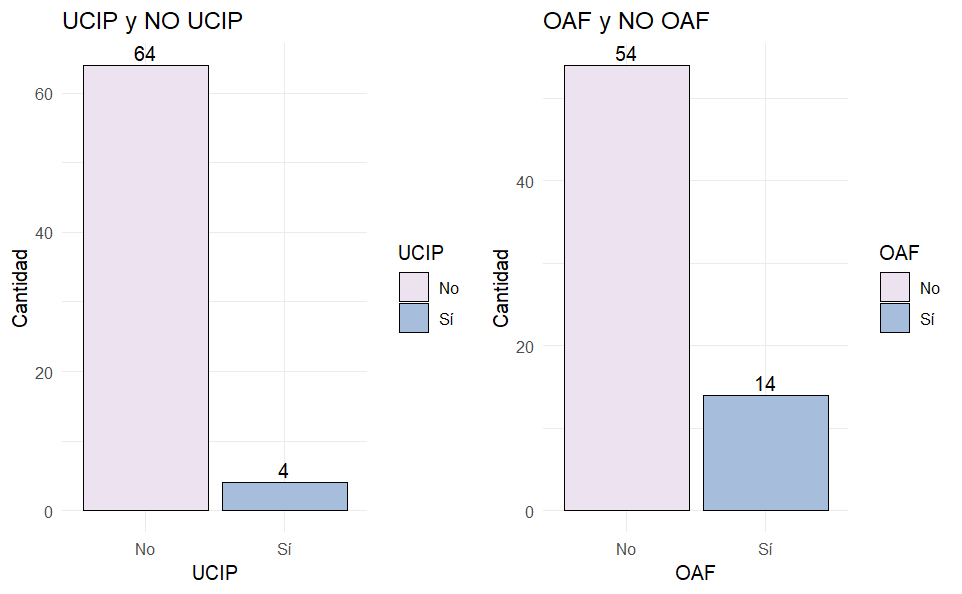
\includegraphics[scale = 0.9]{./img/bar-OAF-UCIP-valid-1.png}
    \caption{Cantidad de pacientes que han sido trasladados a la UCIP y los que NO, que han necesitado OAF y lo que NO, del conjunto de pacientes válidos: \texttt{valid\_patient\_1}}
    \label{fig:bar-OAF-UCIP-valid-1}
\end{figure}

De cara a plantear la investigación teniendo en cuenta los diferentes intervalos antes mencionados, es necesario ver la distribución de los pacientes dentro de los mismos. Esto se puede ver a continuación en la siguiente Figura~\ref{fig:intervalos-valid-1}.

\begin{figure}[H]
    \centering
    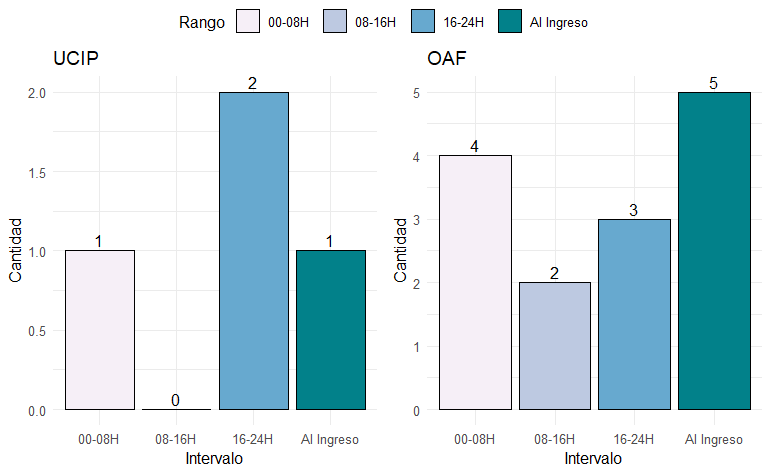
\includegraphics[scale = 0.9]{./img/intervalos-valid-1.png}
    \caption{Distribución de los pacientes dentro de los $3$ intervalos de estudio del conjunto de pacientes: \texttt{valid\_patient\_1}}
    \label{fig:intervalos-valid-1}
\end{figure}

Una vez vista la distribución de los pacientes que presentan UCIP y OAF en los $3$ intervalos de tiempo antes mencionados, cabe preguntarse si tiene sentido plantear el presente trabajo de la forma previamente discutida.

Respecto a los pacientes que son ingresados en la UCIP, se les va a catalogar como pacientes que han sufrido un \textit{Deterioro}. Dado que todos los pacientes que han sido ingresados en la UCIP han recibido soporte respiratorio mediante la técnica OAF, simplemente se les va a considerar como pacientes que han necesitado OAF. En otras palabras, no se utilizará la variable UCIP como variable de salida en este trabajo debido a la escasa representación de este tipo de paciente. Esta consideración se ha mencionado anteriormente en el conjunto total de pacientes en la Figura~\ref{fig:venn-OAF-UCIP} de la Sección~\ref{sec:seleccion_pacientes}.

La exclusión de los pacientes que han sufrido OAF tiene sentido, ya que una vez que al paciente se le suministra OAF, los datos de monitorización recogidos del mismo ya están afectados por la técnica de soporte respiratorio. Por lo tanto, carece de sentido utilizar dichos datos para predecir si el paciente va a necesitar OAF en las próximas $8$ horas, ya que se están recogiendo en un contexto diferente al de los demás pacientes.

Respecto a los pacientes que se les ha aplicado OAF, si excluimos a los pacientes que se les ha aplicado OAF nada más ser ingresados, y aquellos que la han necesitado en las primeras $8$ horas, solo nos quedan 5 pacientes del conjunto de pacientes que han sufrido OAF para realizar el estudio. La falta de presencia de pacientes de este conjunto se va a abordar mediante la técnica de \textit{oversampling-SMOTE} que se explicará en la Sección~\ref{sec:oversampling}.

Una vez explicado el motivo de la exclusión de los pacientes que han sido ingresados en la UCIP y los que han necesitado OAF, se va a proceder a explicar los $2$ estudios que se van a realizar en la Sección~\ref{sec:estudios}.

\subsubsection{Estudios}\label{sec:estudios}

\paragraph{Estudio 1}\label{sec:estudio1}

En el \textit{Estudio 1} se considerará al conjunto de pacientes: \texttt{Valid\_patients\_P1}. En este estudio se pretende observar las posibles diferencias entre las \textit{Series Temporales} de monitorización en función de si el paciente ha sido intervenido con OAF o no. Para ello se va a realizar un análisis de la varianza de las medias de las variables de monitorización (\textit{Frecuencia Cardíaca} y \textit{Saturación de O$_2$}) de los pacientes que han necesitado OAF y los que no.

\paragraph{Estudio 2}\label{sec:estudio2}

En el \textit{Estudio 2} se considerará el conjunto de pacientes: \texttt{Valid\_patients\_P2}. En este estudio se pretende observar si es posible predecir si un paciente va a necesitar OAF en las próximas $8$ horas al ingreso. 

Antes de realizar el modelado del algoritmo de clasificación discreta, se va a querer visualizar si mediante el \textit{clustering} de los valores de monitorización de los pacientes se pueden observar diferencias entre los pacientes que han necesitado OAF y los que no. Para la correcta ejecución de lo anteriormente mencionado se seguirán varios pasos:

\begin{enumerate}
    \item \textbf{Selección de Datos:} Al tener 480 valores de monitorización de \textit{Frecuencia Cardíaca} y \textit{Saturación de O$_2$} se van a utilizar diferentes datos para la ejecución de los clusters:
    \begin{enumerate}
        \item \textsc{Datos en bruto:} Se van a utilizar los 480 datos en bruto de monitorización de los pacientes de cada \textit{Serie Temporal}.
        \item \textsc{Función de autocorrelación (FAC):} Se van a utilizar las primeras 50 observaciones de la FAC de cada \textit{Serie Temporal}.
        \item \textsc{Función de autocorrelación cruzada (FACC):} Se van a utilizar las primeras 100 observaciones de la FACC de la relación entre las \textit{Serie Temporales} de \textit{Frecuencia Cardíaca} y \textit{Saturación de O$_2$}.
        \item \textsc{Periodograma:} Se usarán los periodogramas de cada \textit{Serie Temporal}.
    \end{enumerate}
    \item \textbf{Clustering:} Mediante cluster jerárquico se van a agrupar los pacientes en función de los datos seleccionados en el paso anterior.
    \item \textbf{Visualización:} Se van a visualizar los clusters obtenidos en el paso anterior en función de si el paciente ha necesitado OAF de esta forma se pretenderá ver si se aíslan de alguna forma las dos categorías de pacientes previamente establecidas. 
    \item \textbf{Caracterización de Clusters:} 
    Se llevará a cabo la caracterización de los clusters, tomando en consideración las diversas variables descriptivas de cada paciente (edad, género, peso, OAF, ...). Esto se realizará mediante la construcción de un modelo de clasificación discreta, se buscará entender cómo las distintas variables descriptivas influyen en la asignación de etiquetas a los clusters. Este análisis permitirá identificar las variables más influyentes en la distinción de pacientes pertenecientes a los diferentes clusters. Lo ideal en este caso sería observar como en un cluster la variable OAF es la que más influye en la clasificación de los pacientes, ya que esto significaría que los clusters se han formado en función de si el paciente ha necesitado OAF o no. Si esto es así se podría concluir que los clusters obtenidos partiendo de los datos obtenidos de las \textit{Series Temporales} y sus respectivas transformaciones, son capaces de diferenciar a los pacientes que han necesitado OAF de los que no. Respecto a este punto y en último lugar se va a mostrar como se distribuye la importancia de los datos utilizados en función de las etiquetas utilizadas para realizar el \textit{clustering}.
    \item \textbf{Modelado:} Si el anterior paso resulta exitoso será inmediato generar un modelo que permita la clasificación de pacientes que van a necesitar OAF y los que no. El modelo de clasificación será un modelo de clasificación discreta, ya que la variable de salida es una variable categórica con dos categorías: \textit{paciente que va a necesitar OAF} y \textit{paciente que no va a necesitar OAF}. 
\end{enumerate}


Para ello se va a realizar un análisis de clasificación binaria, donde la variable de salida será si el paciente ha necesitado OAF o no. Para ello se van a utilizar los datos de monitorización de las primeras $8$ horas de monitorización de los pacientes.











\subsubsection{Oversampling}\label{sec:oversampling}

En el campo médico, suele ser común encontrarse con conjuntos de datos donde una categoría tiene significativamente menos observaciones que otra, es decir el conjunto total de la muestra se presenta desbalanceada. Esta disparidad puede afectar negativamente el rendimiento de los modelos de clasificación, ya que pueden tener dificultades para aprender patrones de la clase minoritaria. En el caso de este estudio dónde solo se cuenta con solo 5 pacientes en una categoría (pacientes que ha necesitado OAF posteriormente a las $8$ primeras horas de ingreso) y 40 (paciente que no ha necesitado OAF) de la  otra, existe un claro desequilibrio que puede impactar la precisión de cualquier modelo que se intenta construir.

La técnica utilizada en este trabajo, \textit{SMOTE} (\textit{Synthetic Minority Over-sampling Technique}), es un algoritmo estadístico utilizado para abordar el problema de muestras desbalanceadas en datos de clasificación. En lugar de simplemente duplicar las observaciones de la clase minoritaria, \textit{SMOTE} crea nuevas muestras artificiales interpolando entre observaciones cercanas. Esto se logra eligiendo una observación de la clase minoritaria y generando puntos artificiales en la dirección de sus vecinos más cercanos de la misma categoría. De esta manera, se aumenta el número de observaciones de la clase minoritaria sin simplemente duplicar los mismos puntos (~\cite{Chawla2002}).
\newpage

\subsection{Metodología del Estudio 1}\label{sec:metodologia-estudio-1}

En este primer estudio se realizará un análisis de la varianza de las medias de los datos de monitorización de los pacientes pediátricos; los que han necesitado OAF y a los que no la han necesitado. Este análisis de la varianza de los $68$ pacientes pertenecientes del conjunto de datos \texttt{Valid\_patients\_P1} se hará para cada hora de las $24$ totales de monitorización de los pacientes.

Para dicho análisis se hará uso de la prueba $t$ de Student. Esta es una técnica estadística utilizada para comparar las medias de dos grupos (como se presenta en esta situación) y determinar si las diferencias observadas entre ellas son estadísticamente significativas. Se basa en calcular un estadístico $t$ que mide la diferencia entre las medias en términos de la variabilidad dentro de los grupos.

Supongamos que tenemos dos poblaciones, $X$ e $Y$, de las que se han obtenido muestras aleatorias simples con tamaños $n$ y $m$, respectivamente. La hipótesis nula y alternativa se plantean de la siguiente manera:

Hipótesis Nula ($H_0$):
\[
\mu_X = \mu_Y
\]

Hipótesis Alternativa ($H_1$):
\[
\mu_X \neq \mu_Y \quad \text{o} \quad \mu_X < \mu_Y \quad \text{o} \quad \mu_X > \mu_Y
\]

La distribución \( t \) de Student con \( v \) grados de libertad puede definirse como la distribución de la variable aleatoria \( T \) definida por:

\[ T := \frac{Z}{\sqrt{\frac{X}{v}}} \sim t_v \]

donde:

\( Z \sim N(0,1) \) es una variable aleatoria con distribución normal estándar (distribución normal con media 0 y varianza 1).

\( X \sim \chi_{v}^{2} \) es una variable aleatoria que sigue una distribución chi-cuadrada con \( v \) grados de libertad.

\( Z \) y \( X \) son variables aleatorias independientes.

El estadístico \( t \) calculado se compara con un valor crítico de la distribución \( t \) de Student con \( n+m-2 \) grados de libertad para determinar si las diferencias entre las medias son estadísticamente significativas. Si el valor \( p \) asociado con el estadístico \( t \) es menor que el umbral predefinido (nivel de significancia \( \alpha \)), se rechaza la hipótesis nula y se concluye que hay una diferencia significativa entre las medias.


Este estudio se va a realizar para la \textit{Frecuencia Cardiaca}, para la \textit{Frecuencia Cardiaca Transformada por Cuantiles}, para la \textit{Frecuencia Cardiaca Escalada} y para la \textit{Saturación de Oxígeno Escalada}. Se quiere pues observar si realmente existe una diferencia significativa entre las medias de los datos de monitorización de los pacientes pediátricos que han necesitado OAF y los que no la han necesitado.

Para ello partiendo de los $1440$ valores de monitorización se calcularán las medias horarias gracias al código mostrado en la Sección~\ref{sec:anexo2} de los Anexos.




\newpage


\subsection{Metodología Estudio 2}\label{sec:metodologia-estudio-2}

En este segundo estudio como se ha mencionado en la Sección~\ref{sec:estudio2}, se tomará en cuenta el conjunto de pacientes: \texttt{Valid\_patients\_P2}. El propósito de este estudio es investigar la viabilidad de predecir si un paciente requerirá Oxigenoterapia de Alto Flujo (OAF) en las siguientes $8$ horas después del ingreso del paciente.

Para ello habrá que utilizar $2$ herramientas estadísticas que permitan realizar la predicción de la variable de interés:

\begin{itemize}
    \item \textbf{Hierarchical Clustering(HCLUST):} En primer lugar, de manera exploratoria, se agruparán los pacientes en función de las distancias euclídeas entre ellos utilizando el método de clustering \texttt{hclust}. Posteriormente, se evaluará si los grupos generados han aislado en un \textit{cluster} a los pacientes con necesidad de Oxigenoterapia de Alto Flujo (OAF) de aquellos que no la requieren.
    \item textbf{Random Forest Classification (RF):} En segundo lugar, se aplicará el método estadístico \textit{Random Forest} para clasificar a los pacientes según el cluster al que pertenecen, utilizando las variables descriptivas de la Tabla~\ref{tabla:cuali_cuanti}. En este proceso, no se emplearán las variables de \textit{Notas} ni el \textit{Identificador Paciente}. Si se logra aislar a los pacientes que han necesitado OAF, se determinará la importancia directa de la variable \textit{Deterioro}, la cual indica si el paciente ha experimentado OAF o no.
\end{itemize}

\subsubsection{Hierarchical Clustering (HCLUST)}\label{sec:hclust}

Hierarchical Clustering (HCLUST) es una técnica de análisis de datos utilizada para agrupar objetos en función de sus similitudes o distancias. Esta técnica se basa en la construcción de un dendrograma, una estructura jerárquica de ramas que representa la agrupación gradual de los datos (\cite{jain1988algorithms}).

El proceso comienza considerando cada objeto como un grupo individual y luego fusionando iterativamente los grupos más cercanos en función de una medida de similitud o distancia. La distancia puede ser calculada de varias formas, siendo las más comunes y sencilla la distancia euclidiana: 

La fórmula general para calcular la distancia euclídea entre dos objetos \(x_p \) y \(x_q\) es:

\[
d_{euc}(p,q) = \sqrt{(x_p - x_q)^2 + (y_p - y_q)^2}
\]

Esta ecuación puede generalizarse para un espacio euclídeo n-dimensional donde cada punto está definido por un vector de n coordenadas: $p = (p_1,p_2,p_3,...,p_n)$

\[
d_{euc}(p,q) = \sqrt{(p_1 - q_1)^2 + (p_2 - q_2)^2 + \ldots + (p_n - q_n)^2} = \sqrt{\sum_{i=1}^{n}(p_i - q_i)^2}
\]

Hay diferentes distancias que se pueden usar e función del propósito de lo que se quiera hacer con los datos. Cada uno de ellos depende del tipo de datos que se esté utilizando. Se mostrará a continuación una pequeña selección de lo que está disponible en \texttt{R}.
\begin{table}[H]
    \centering
    \caption{Opciones de método de distancia}
    \begin{tabular}{|p{3cm}|p{2.5cm}|p{4.5cm}|p{6cm}|}
    \hline
    \textbf{Medida} & \textbf{Método} & \textbf{Mejor utilizado para...} & \textbf{Cálculo} \\
    \hline
    Distancia euclidiana & euclidean & Datos continuos & \(edist(x, y) = \sqrt{((x_1 - y_1)^2 + (x_2 - y_2)^2 + \ldots)}\) \\
    \hline
    Distancia de Hamming & hamming & Datos categóricos & \(hdist(x, y) = \sum((x_1 \neq y_1) + (x_2 \neq y_2) + \ldots)\) \\
    \hline
    Distancia de Manhattan & manhattan & Diferencias absolutas entre componentes correspondientes & \(mdist(x, y) = \sum(|x_1 - y_1| + |x_2 - y_2| + \ldots)\) \\
    \hline
    Distancia de Canberra & canberra & Valores no negativos (ej. conteos) & \(cdist(x, y) = \sum\left(\frac{|x - y|}{|x + y|}\right)\) \\
    \hline
    Distancia binaria asimétrica de Jaccard & binary & Datos binarios & \(j.dist(x, y) = b + c + d\) (Usando tabla siguiente) \\
    \hline
    \end{tabular}
\end{table}

Una vez que se haya creado una matriz de distancias, es necesario decirle al modelo \textit{HCLUST} que debe entender él como similitud. Esto lleva al próximo punto de decisión: seleccionar qué se entender por \textit{similitud} entre pacientes.

Existen muchas opciones para calcular similitudes entre observaciones. Los métodos \textit{ward.D} y \textit{ward.D2} son generalmente populares y efectivos. Sin embargo, aquí se mostrarán algunas otras opciones diferentes. A continuación se muestra una lista de los métodos de similitud más comunes:

\begin{table}[H]
    \centering
    \begin{tabular}{|p{3.5cm}|p{6cm}|p{6cm}|}
    \hline
    \textbf{Método} & \textbf{Proceso} & \textbf{Resultado} \\
    \hline
    Single & Mide la distancia entre los dos puntos más cercanos en cada cluster & Generalmente es mejor para identificar valores atípicos que no se agrupan bien \\
    \hline
    Complete & Mide la distancia entre los dos puntos más distantes en cada cluster & Generalmente produce clusters más compactos \\
    \hline
    Centroid & Mide la distancia entre el centro de cada cluster & Generalmente funciona mejor para datos con menos similitudes \\
    \hline
    Mediana & Mide la distancia mediana entre el punto mediano de cada cluster & Similar al centroide, pero ponderado hacia donde se encuentran la mayoría de las observaciones \\
    \hline
    Promedio & Mide la distancia promedio entre cada observación en cada cluster, ponderado por el número de observaciones en cada cluster & Generalmente similar a enlace completo, mejor para incorporar valores atípicos \\
    \hline
    Mcquitty & Similar al promedio, pero no toma en cuenta el número de puntos en el cluster & Generalmente similar a enlace simple \\
    \hline
    Ward.D & Minimiza la varianza dentro de los clusters (suma de errores). Combina clusters según la menor distancia entre clusters & Generalmente produce clusters más compactos \\
    \hline
    Ward.D2 & Igual que Ward.D, pero las diferencias están al cuadrado (suma de errores al cuadrado) & Enfatiza las diferencias identificadas en Ward.D, haciendo que los clusters sean más diferenciables \\
    \hline
    \end{tabular}
    \caption{Métodos de enlace y sus resultados}
\end{table}

Una vez establecido que se entiende como similitud el resultado final se muestra en forma de deprograma dónde los pacientes se agrupan gradualmente. Se puede seleccionar el número de grupos al cortar el dendrograma en diferentes alturas. Hay algoritmos que son capaces de calcular el número de grupos más óptimo a considerar como \textit{silouhette} (Sección~\ref{sec:silhouette}) o \textit{gap statistic} que al final son puntuaciones que varían en función del número de \textit{clusters} que se haya decidido previamente.

\textit{HCLUST} tiene la ventaja de ser visualmente intuitivo y permite explorar la estructura de los datos a diferentes niveles de detalle. Sin embargo, su complejidad computacional puede ser alta en conjuntos de datos grandes.

En el contexto de este estudio, se utilizará el método de clustering \textit{HCLUST} para agrupar a los pacientes según sus distancias euclídeas considerando como similitud entre pacientes el método \textit{Ward.D2}. Esto permitirá investigar si los grupos generados pueden destacar diferencias entre pacientes que requieren Oxigenoterapia de Alto Flujo (OAF) y aquellos que no la necesitan.

\paragraph{Silhouette}\label{sec:silhouette}

El método de \textit{Silhouette} es una técnica utilizada para determinar el número óptimo de clusters en un análisis cluster. Proporciona una medida de cómo de similar es un objeto a su propio cluster (cohesión) en comparación con otros clusters (separación). La puntuación de \textit{Silhouette} varía entre -1 y 1, donde una puntuación más alta indica que el objeto está bien ajustado a su propio cluster y mal ajustado a clusters vecinos (\cite{rousseeuw1987silhouettes}).

La fórmula para calcular la puntuación de \textit{Silhouette} \(s(i)\) para un objeto \(i\) se define como:

\[ s(i) = \frac{b(i) - a(i)}{\max\{a(i), b(i)\}} \]

Donde:
\begin{itemize}
    \item \(a(i)\) es la distancia promedio entre el objeto \(i\) y todos los demás objetos en el mismo cluster (cohesión).
    \item \(b(i)\) es la distancia promedio entre el objeto \(i\) y todos los objetos en el cluster más cercano al que \(i\) no pertenece (separación).
\end{itemize}

La puntuación de \textit{Silhouette} para un conjunto de datos se puede calcular promediando las puntuaciones de silueta de todos los objetos:

\[ \text{Puntuación de Silhouette Media} = \frac{1}{N} \sum_{i=1}^{N} s(i) \]

Donde \(N\) es el número total de objetos en el conjunto de datos.

El número óptimo de clusters se elige cuando la puntuación de \textit{Silhouette} media es máxima. Se busca el número de clusters que produce una mayor cohesión dentro de los clusters y una mayor
separación entre los clusters vecinos, lo que refleja en una puntuación \textit{Silhouette} más alta.


\subsubsection{Random Forest (RF)}\label{sec:rf}

Los Random Forest, también conocidos como bosques aleatorios, consisten en un conjunto de árboles de clasificación. Estos bosques se crean mediante un algoritmo que introduce variabilidad en los datos y las variables utilizadas, con el objetivo de reducir la correlación entre los árboles.

El objetivo de los Random Forest es predecir una variable respuesta \(y_i\) en función de \(p\) variables explicativas \(x_i = (x_{1i}, x_{2i}, \ldots, x_{pi})^T\), donde \(N\) es el número total de observaciones en el conjunto de datos. El conjunto utilizado para la estimación se llama \(d = (X, y)\)(\cite{ho1995random}).


\paragraph{CART: Árboles de Clasificación y Regresión}
Los árboles de clasificación (CART) son la base de los algoritmos Random Forest. Estos dividen o segmentan el espacio de los predictores en un número limitado de regiones. Este enfoque pertenece al aprendizaje supervisado, donde se tiene una variable objetivo y se busca establecer una función clasificadora para predecir su valor. CART (Classification and Regression Trees) es una técnica que permite construir árboles de clasificación y de regresión. Se utiliza clasificación cuando la variable objetivo es discreta y regresión cuando es continua.

Dado un conjunto inicial de datos, un árbol de clasificación se construye creando una serie de particiones binarias. Cada partición se llama nodo y divide el espacio en dos partes según una variable. El objetivo es imponer restricciones a los datos a medida que descienden niveles en el árbol para clasificarlos en diferentes conjuntos (\cite{wu2008top}).

Para desarrollar un árbol, es necesario definir dos aspectos:
\begin{itemize}
	\item Cómo se selecciona el criterio de partición de un nodo.
	\item Criterios de parada que determinan cuándo finaliza el proceso de subdivisión.
\end{itemize}


\subparagraph{Criterio de Partición}
Supongamos que tenemos \(p\) variables explicativas o predictores: \(x_1, x_2, \ldots, x_p\). Tomemos la primera variable \(x_1\) y busquemos el valor \(s\) que divide la muestra en dos regiones que cumplan:

\[
R1 = \{x_{1i} \mid x_{1i} < s\} \quad \text{y} \quad R2 = \{x_{1i} \mid x_{1i} \geq s\}
\]

Es decir, o se toma una de las variables explicativas (o predictores) de tus datos y se busca un valor $s$ que divida las observaciones en dos grupos: uno donde los valores de esa variable son menores que $s$ y otro donde son mayores o iguales a $s$.

Y que minimice:

\[
RSS_1(s) = \sum_{i \in R_1} (y_i - \bar{y}_{R_1})^2 + \sum_{i \in R_2} (y_i - \bar{y}_{R_2})^2
\]
Donde \(\bar{y}_{R_1}\) y \(\bar{y}_{R_2}\) son las medias de la variable \(y\) en las regiones \(R_1\) y \(R_2\). Esto se hace pues se pretende que en cada grupo la variable respuesta \(y\) sea lo más homogénea posible. Se busca la variable $s$ que minimice la suma de los cuadrados de las diferencias entre los valores de $y$ y la media de $y$ en cada grupo.

Elegido \(s\) óptimo para \(x_1\), se repite el proceso con \(x_1, x_2, \ldots, x_p\). De las \(p\) variables, se elige para la partición la que resulte en la menor \(RSS_j\).

El proceso se repite, pero ahora se tratan de manera independiente los conjuntos \(R_1\) y \(R_2\). El proceso continúa hasta que se alcance el criterio preestablecido de parada y se definan los nodos terminales \(R_1^*, R_2^*, \ldots, R_j^*\). El objetivo es lograr una partición de estos nodos que minimice:

\[
RSS_T = \sum_{j=1}^{J} \sum_{i \in R_j^*} (y_i - \bar{y}_{R_j^*})^2
\]

\subparagraph{Criterio de Parada}
Existen varios criterios de parada para limitar el crecimiento del árbol:
\begin{itemize}
	\item Parámetro de Complejidad: Este parámetro se refiere al aumento en el valor de \(R^2\) al agregar una rama al árbol. Se establece un umbral para el cual agregar más ramas al árbol no aumenta significativamente el valor de \(R^2\).
	\item Minsplit: Se detiene el crecimiento del árbol cuando el número de observaciones en un nodo es menor que un umbral predefinido.
	\item Maxdepth: Se detiene el crecimiento cuando la profundidad de las ramas del árbol supera un umbral establecido.
\end{itemize}
La recomendación general es encontrar el árbol más pequeño que maximice el valor de \(R^2\).

\subparagraph{Ventajas de los CART}
Los árboles CART presentan varias ventajas:
\begin{itemize}
	\item No se requiere preparación de los datos de entrada.
	\item Pueden manejar variables faltantes.
	\item Son efectivos para grandes bases de datos con diversas variables.
	\item Son fáciles de entender e interpretar.
\end{itemize}

\subsubsection{Algoritmo de creación del Random Forest}

Para \(b = 1,2, \ldots, B\), se realiza lo siguiente:
- Se elige una muestra de tamaño \(N\) de manera aleatoria y con reemplazo del conjunto de datos total. Esto se llama bootstrap.
- Se construye un árbol llamado \(r_b(x)\), y en cada nodo del árbol se utilizan \(m \ll p\) variables de las \(p\) variables del conjunto de datos. La elección común para \(m\) es \(m = \sqrt{p}\).
- El conjunto de árboles formados, \(r_b(x)\) para \(b = 1,2, \ldots, B\), se llama Random Forest.

\paragraph{División del conjunto de datos}

En general, los algoritmos de Machine Learning dividen el conjunto de datos en dos partes: una para estimación o entrenamiento, y la otra para test o validación.

\paragraph{DEstimación del error en la predicción de variables de respuestas continuas}

La predicción para \(x_i = (x_{1i}, x_{2i}, \ldots, x_{pi})^T\) se calcula como:

\[ \hat{y}_i = \hat{r}_{rf}(x_i) = \frac{1}{B} \sum_{b=1}^{B} \hat{r}_b(x_i) \]

Donde \(B\) es el número de árboles en el Random Forest.

El error se define como:

\[ e_i = y_i - \hat{y}_i \]

El error cuadrático medio (MSE) se calcula como:

\[ MSE = \frac{1}{n} \sum_{i=1}^{n} e_i^2 \]

El coeficiente \(R^2\) se define como:

\[ R^2 = 1 - \frac{\sum_{i=1}^{n} e_i^2}{\sum_{i=1}^{n} (y_i - \bar{y})^2} \]

La desviación típica residual \(S_{\hat{R}}\), siendo \(m\) el número de observaciones en el conjunto de validación, se calcula como:

\[ S_{\hat{R}} = \sqrt{\frac{e_i^2}{m-1}} \]

\paragraph{OOB error (Error fuera de la bolsa)}\label{sec:oob}

El OOB error es una medida de error aplicada a modelos que utilizan la técnica de boostrapping. Dado que aproximadamente \(1/3\) de los datos nunca se seleccionan debido al reemplazo, el OOB representa el error de predicción cometido por el Random Forest en los valores que quedaron fuera de la muestra.

\paragraph{Importancia de las variables}\label{sec:importancia-variables}

Un modelo Random Forest funciona como una caja negra y proporciona buenas predicciones. Sin embargo, no brinda información sobre cada variable explicativa.

La importancia de una variable se puede calcular en función de cómo afecta a la salida del modelo cuando se realizan cambios en las variables de entrada. A continuación, se describen dos formas de calcular la importancia.

\subparagraph{Índice de la pureza de los nodos}

En el contexto de Random Forest, el Índice de la Pureza de los Nodos se refiere al proceso de evaluación de la contribución de cada variable al proceso de particionamiento de los datos en los nodos de cada árbol. Al utilizar una variable en un nodo, se cuantifica la reducción de la variabilidad explicada por la partición resultante. Estos valores de reducción se acumulan para todas las variables y árboles, generando una medida conocida como la importancia de la variable. Las variables que exhiben una mayor capacidad para reducir la variabilidad en los nodos se consideran más importantes en el proceso de toma de decisiones del Random Forest.

\subparagraph{Incremento del Mean Squared Error  \texttt{\%IncMSE}}

El índice \texttt{\%IncMSE} en el contexto de Random Forest mide el incremento en el Error Cuadrático Medio (MSE) a través de la realización de una permutación aleatoria en una de las variables de entrada. La disparidad entre el MSE antes y después de la permutación se normaliza y se promedia para determinar la relevancia de la variable en el proceso de modelado. Este índice proporciona una evaluación cuantitativa de cómo la perturbación de una variable afecta la precisión de las predicciones, identificando así las variables que tienen un mayor impacto en los resultados del Random Forest. Una variable que su permutación genere una gran variación será considerada como importante. Por el contrario, una variable que no afecte la precisión de las predicciones será considerada como no importante.

En resumen, los Random Forest son una poderosa técnica de aprendizaje automático que combina múltiples árboles de clasificación para realizar predicciones más precisas y robustas. Su proceso de creación introduce variabilidad y utiliza técnicas como el OOB error y la importancia de variables para mejorar su rendimiento y capacidad de generalización.

\newpage
\newpage

%%%%%%%%%%%%%%%%%% - TITULOS - %%%%%%%%%%%%%%%%%%

\section{TÍTULOS} \label{sec:titulos}

En los documentos de clase \texttt{article} (los distintos tipos de documentos disponibles así como sus diferentes aplicaciones pueden consultarse en \url{https://en.wikibooks.org/wiki/LaTeX/Document_Structure#Document_classes}) existen por defecto tres profundidades de títulos numerados, en orden jerárquico: \texttt{\textbackslash section}, \texttt{\textbackslash subsection} y \texttt{\textbackslash subsubsection}. El título del presente capítulo es un ejemplo de título de profundidad 1 (comando \texttt{\textbackslash section}).


\subsection{Profundidad 2}

Este es un ejemplo de título de profundidad 2 (comando \texttt{\textbackslash subsection}) que, como se puede ver, queda automáticamente numerado con respecto al título jerárquicamente superior (profundidad 1) inmediatamente anterior.


\subsubsection{Profundidad 3}

Este es un ejemplo de título de profundidad 3 (comando \texttt{\textbackslash subsubsection}) que, de nuevo, se numera automáticamente con respecto al título jerárquicamente superior (profundidad 2) inmediatamente anterior.


\paragraph{Profundidad 4}

En este documento se añade una profundidad de títulos numerados adicional (mediante los comandos \texttt{\textbackslash setcounter\{secnumdepth\}\{4\}} y \texttt{\textbackslash setcounter\{tocdepth\}\{4\}}, ver preámbulo para más información). Así, el comando \texttt{\textbackslash paragraph} se utiliza para incorporar títulos de profundidad 4, como en el caso del título del presente apartado. 

Si se quisiera aumentar en un grado más la profundidad de títulos, bastaría con asignar el valor 5 a ambos comandos \texttt{\textbackslash setcounter} (\texttt{\textbackslash setcounter\{secnumdepth\}\{5\}} y \texttt{\textbackslash setcounter\{tocdepth\} \{5\}}), y realizar los cambios pertinentes en el comando \texttt{\textbackslash subparagraph} de modo que su formato sea coherente con el del resto de títulos (de la misma forma que lo realizado con el comando \texttt{\textbackslash paragraph}, ver preámbulo para más información)


\subsection{Formato y numeración}

La numeración así como el formato de los títulos (tamaño de fuente, tipografía, etc.) utilizados en este documento corresponden a los valores por defecto (excepto en el caso de \texttt{\textbackslash paragraph}, como se explica más arriba), pero pueden ser modificados en el preámbulo del documento (una breve guía sobre la personalización del formato de los títulos puede consultarse en \url{https://www.overleaf.com/learn/latex/sections_and_chapters#Customize_chapters_and_sections}). 

En caso de que no se quiera numerar alguno de los títulos, basta con añadir un asterísco (\textbf{*}) al comando correspondiente, como por ejemplo \texttt{\textbackslash subsection*\{Título sin numerar\}}:


\subsection*{Título sin numerar} 
\addcontentsline{toc}{subsection}{Título sin numerar}

Los títulos sin numerar no aparecen en la tabla de contenidos (índice), pero pueden ser añadidos con ayuda del comando \texttt{\textbackslash addcontentsline\{toc\}} (utilizado previamente para los apartados de Agradecimientos y Resumen ejecutivo), que en este caso quedaría como: \texttt{\textbackslash addcontentsline\{toc\} \ \{subsection\}\{Título sin numerar\}}.


\subsection{Referencias con el comando \text\textbackslash label} \label{sec:referencias}

Los comandos \texttt{\textbackslash label} se utilizan en \LaTeX \ para colocar referencias que puedan ser utilizadas a lo largo del documento. Son especialmente útiles, como se verá más adelante, para referirse a elementos del documento como tablas, imágenes, diagramas, etc., pero también pueden ser utilizados para referirse a capítulos o secciones del informe. 

Para citar una referencia basta con utilizar el comando \texttt{\textbackslash ref} en el interior del cual se indica aquello a lo que se quiere hacer referencia, como por ejemplo al primer capítulo de este documento, el capítulo \ref{sec:titulos}.

\textbf{Nota:} ya que el comando \texttt{\textbackslash label} es compartido por títulos, figuras, tablas, etc., es bastante útil utilizar una nomenclatura clara para definir cada referencia, por ejemplo: ``tab:" \ seguido del nombre de la tabla para las tablas, ``fig:" \ seguido del nombre de la figura para las figuras, etc.

%%%%%%%%%%%%%%%%%%%%%%%%%%%%%%%%%%%%%%%%%%%%%%%%%%


%%%%%%%%%%%%%% - FORMATO DE TEXTO - %%%%%%%%%%%%%%

\newpage
\section{FORMATO DE TEXTO}\label{sec:formato}

Como en cualquier editor de texto, el formato del texto puede alterarse sobre la marcha de distintas maneras. Pueden incluirse palabras en \textbf{negrita} (si se utiliza Overleaf puede utilizarse el atajo \texttt{ctrl+B} en Windows o \texttt{Cmd+B} en Mac), palabras en \textit{curiva} (\texttt{ctrl+I} o \texttt{Cmd+I}), o una \textit{\textbf{combinación}} de ambas.


\subsection{Tamaño de fuente}

También se puede modificar el {\huge tamaño} de forma {\footnotesize rápida} y {\Large sencilla} (una lista con los distintos tamaños y sus comandos respectivos puede encontrarse en \url{https://www.sascha-frank.com/latex-font-size.html})


\subsection{Color}

\definecolor{coral}{rgb}{1.0, 0.5, 0.31}

El \textcolor{teal}{color} del \textcolor{purple}{texto} también puede ser modificado sobre la marcha, así como subrayar ciertas \colorbox{lightgray}{palabras} o \colorbox{yellow}{bloques de palabras}. Algunos colores están implementados por defecto y pueden utilizarse indicando simplemente su denominación (red, orange, blue, etc., resumidos en esta \href{https://i.stack.imgur.com/tmoHS.png}{\textcolor{blue}{imagen}}), pero también pueden definirse colores mediante sus códigos rgb, RGB, HTML, o cmyk, haciendo uso del paquete \texttt{xcolor}. Por ejemplo: \textbackslash \texttt{definecolor\{coral\}\{rgb\}\{1.0, 0.5, 0.31\}\definecolor{coral}{rgb}{1.0, 0.5, 0.31}} define un color con el correspondiente identificador rgb que se puede utilizar de ahora en adelante haciendo uso del nombre que se le ha asignado, \textcolor{coral}{coral} (una extensa guía con gran variedad de colores puede consultarse en \url{http://latexcolor.com/})


\subsection{Espaciado}

Puede ser de utilidad insertar \hspace{0.5cm} espacios \hspace{1cm} entre distintas \hspace{2cm} palabras, o espacios verticales entre párrafos u otros elementos del documento,

\vspace{6cm}

como en este caso.

Aunque \textbackslash\texttt{hspace} y \textbackslash\texttt{vspace} presenten la ventaja de ser totalmente personalizables, para espaciados de tamaño estándar es recomendable utilizar \textbackslash \ (espacio) y \textbackslash\textbackslash \ (salto de línea).


\subsection{Listas}

Existen dos tipos de listas, las numeradas y las no numeradas.


\subsubsection{Listas no numeradas}

Las listas no numeradas corresponden al entorno \texttt{itemize}:

\begin{itemize}
    \item Primer elemento.
    \item Segundo elemento.
\end{itemize}

Se pueden hacer listas de distintos niveles de profundidad:

\begin{itemize}
    \item Primer elemento.
    \item Segundo elemento.
    \begin{itemize}
        \item Tercer elemento.
        \begin{itemize}
            \item Cuarto elemento.
            \item Quinto elemento.
        \item Sexto elemento.
        \end{itemize}
        \item Séptimo elemento.
        \begin{itemize}
            \item Octavo elemento.
        \end{itemize}
    \end{itemize}
    \item Noveno elemento.
\end{itemize}


\subsubsection{Listas numeradas}

Las listas numeradas corresponden al entorno \texttt{enumerate}:

\begin{enumerate}
    \item Primer elemento
    \item Segundo elemento
    \item Tercer elemento
\end{enumerate}

Del mismo modo, las listas numeradas pueden incorporar distintos niveles de profundidad:

\begin{enumerate}
    \item Primer elemento
    \begin{enumerate}
        \item Segundo elemento
        \item Tercer elemento
        \begin{enumerate}
            \item Cuarto elemento
            \begin{enumerate}
                \item Quinto elemento
                \item Sexto elemento
            \end{enumerate}
            \item Séptimo elemento
        \end{enumerate}
        \item Octavo elemento
        \item Noveno elemento
    \end{enumerate}
    \item Décimo elemento.
\end{enumerate}


\subsubsection{Listas combinadas}

Las listas numeradas y no numeradas pueden combinarse, por ejemplo:

\begin{itemize}
    \item Primer elemento.
    \begin{enumerate}
        \item Segundo elemento
        \item Tercer elemento
        \begin{itemize}
            \item Cuarto elemento
            \item Quinto elemento
            \begin{enumerate}
                \item Sexto elemento
                \item Séptimo elemento
            \end{enumerate}
            \item Octavo elemento
        \end{itemize}
        \item Noveno elemento
    \end{enumerate}
    \item Décimo elemento
\end{itemize}


\subsubsection{Formato de las listas}

Tanto el estilo de las distintas numeraciones dentro de una lista numerada como la apariencia de los \textit{bullet points} de las listas no numeradas pueden personalizarse:

\renewcommand{\labelenumi}{\Roman{enumi}} % Primera profundidad de la lista numerada: números romanos (\Roman)
\renewcommand{\labelenumii}{\Alph{enumii}} % Segunda profundidad de la lista numerada: letras en mayúsculas (\Alph)
\renewcommand{\labelitemi}{\textbullet} % Primera profundidad de la lista no numerada: puntos (\textbullet).
\renewcommand{\labelitemii}{\textasteriskcentered} % Segunda profundidad de la lista no numerada: asteriscos (\textasteriskcentered) 

\begin{itemize}
    \item Primer elemento.
    \begin{enumerate}
        \item Segundo elemento
        \item Tercer elemento
        \begin{itemize}
            \item Cuarto elemento
            \item Quinto elemento
            \begin{enumerate}
                \item Sexto elemento
                \item Séptimo elemento
            \end{enumerate}
            \item Octavo elemento
        \end{itemize}
        \item Noveno elemento
    \end{enumerate}
    \item Décimo elemento
\end{itemize}

Los distintos formatos posibles pueden consultarse en la guía elaborada por Overleaf que puede encontrarse en \url{https://www.overleaf.com/learn/latex/lists}.

%%%%%%%%%%%%%%%%%%%%%%%%%%%%%%%%%%%%%%%%%%%%%%%%%%


%%%%%%%%%%%%%%%%%%% - TABLAS - %%%%%%%%%%%%%%%%%%%

\newpage
\section{TABLAS} \label{sec:tablas}

Las tablas se definen en el entorno \texttt{table}. Existen infinidad de posibilidades en cuanto a su formato: omitir o dibujar líneas horizontales y verticales, fusionar columnas y filas, alinear el contenido a la derecha, izquierda o centro, y demás opciones resumidas en \url{https://www.overleaf.com/learn/latex/tables}. Dado que la forma de construir una tabla directamente en código \LaTeX \ está lejos de ser cómoda e intuitiva, quizás lo más recomendable sea acudir a editores de tablas que generan automáticamente el código correspondiente y cuya interfaz es similar a la que puede encontrarse en Excel, como por ejemplo \url{https://www.tablesgenerator.com/}. Un ejemplo sencillo de tabla se muestra a continuación:

\vspace{25pt}

\begin{table}[H]
\centering
\begin{tabular}{|c|c|c|l|}
\hline
$\bm{n}$ & $\bm{a_n}$ & $\bm{a_{n+1}}$ & $\bm{\varphi} \ _{(= a_{n+1}/a_n)}$ \\ \hline\hline
\textbf{1} & 1 & 1 & 1 \\ \hline
\textbf{2} & 1 & 2 & 2 \\ \hline
\textbf{3} & 2 & 3 & 1,5 \\ \hline
\textbf{4} & 3 & 5 & 1,66666667 \\ \hline
\textbf{5} & 5 & 8 & 1,6 \\ \hline
\textbf{6} & 8 & 13 & 1,625 \\ \hline
\textbf{7} & 13 & 21 & 1,61538462 \\ \hline
\textbf{8} & 21 & 34 & 1,61904762 \\ \hline
\textbf{9} & 34 & 55 & 1,61764706 \\ \hline
\textbf{10} & 55 & - & - \\ \hline
\end{tabular}
\caption{Cinco primeros términos de la sucesión de Fibonacci}
\label{tabla:fibonacci5}
\end{table}

\vspace{5pt}

El título de la tabla se indica mediante el comando \textbackslash\texttt{caption} (este comando no solamente sirve para añadir un título a la tabla, sino que es esencial para que ésta aparezca en el índice de tablas), y, al igual que en el caso de los títulos de capítulos (ver apartado \ref{sec:referencias}), es muy recomendable añadir el comando \textbackslash\texttt{label} para poder referirse a la tabla en cuestión en partes posteriores (o anteriores) del documento.


\subsection{Posicionamiento}

Las tablas (al igual que otros elementos como imágenes o diagramas, como se verá más adelante) pueden posicionarse en distintos lugares de la página y en distintas posiciones con respecto al texto. La forma más común de situar una tabla es inmediatamente después de un párrafo y centrada en la página (como en el caso de la tabla \ref{tabla:fibonacci5}), lo que se consigue indicando \texttt{[H]} al iniciar el entorno \texttt{table} y añadiendo el comando \textbackslash\texttt{centering}, respectivamente. Una guía que recopila las distintas opciones en lo que se refiere al posicionamiento de tablas e imágenes puede consultarse en \url{https://www.overleaf.com/learn/latex/positioning_images_and_tables}.


\newpage
\subsection{Entorno \textbackslash\texttt{longtable}}

En el caso de que una tabla sea demasiado larga como para caber en una única página se puede utilizar el entorno \texttt{longtable}, mediante el cual \LaTeX \ secciona la tabla de forma automática en tantas partes como sea necesario.

\vspace{10pt}

\begin{longtable}[H]{|c|c|c|l|}
\hline
$\bm{n}$ & $\bm{a_n}$ & $\bm{a_{n+1}}$ & $\bm{\varphi} \ _{(= a_{n+1}/a_n)}$ \\ \hline\hline
\endhead
\textbf{1} & 1 & 1 & 1 \\ \hline
\textbf{2} & 1 & 2 & 2 \\ \hline
\textbf{3} & 2 & 3 & 1,5 \\ \hline
\textbf{4} & 3 & 5 & 1,66666667 \\ \hline
\textbf{5} & 5 & 8 & 1,6 \\ \hline
\textbf{6} & 8 & 13 & 1,625 \\ \hline
\textbf{7} & 13 & 21 & 1,61538462 \\ \hline
\textbf{8} & 21 & 34 & 1,61904762 \\ \hline
\textbf{9} & 34 & 55 & 1,61764706 \\ \hline
\textbf{10} & 55 & 89 & 1,61818182 \\ \hline
\textbf{11} & 89 & 144 & 1,61797753 \\ \hline
\textbf{12} & 144 & 233 & 1,61805556 \\ \hline
\textbf{13} & 233 & 377 & 1,61802575 \\ \hline
\textbf{14} & 377 & 610 & 1,61803714 \\ \hline
\textbf{15} & 610 & 987 & 1,61803279 \\ \hline
\textbf{16} & 987 & 1597 & 1,61803445 \\ \hline
\textbf{17} & 1597 & 2584 & 1,61803381 \\ \hline
\textbf{18} & 2584 & 4181 & 1,61803406 \\ \hline
\textbf{19} & 4181 & 6765 & 1,61803396 \\ \hline
\textbf{20} & 6765 & 10946 & 1,618034 \\ \hline
\textbf{21} & 10946 & 17711 & 1,61803399 \\ \hline
\textbf{22} & 17711 & 28657 & 1,61803399 \\ \hline
\textbf{23} & 28657 & 46368 & 1,61803399 \\ \hline
\textbf{24} & 46368 & 75025 & 1,61803399 \\ \hline
\textbf{25} & 75025 & 121393 & 1,61803399 \\ \hline
\textbf{26} & 121393 & 196418 & 1,61803399 \\ \hline
\textbf{27} & 196418 & 317811 & 1,61803399 \\ \hline
\textbf{28} & 317811 & 514229 & 1,61803399 \\ \hline
\textbf{29} & 514229 & 832040 & 1,61803399 \\ \hline
\textbf{30} & 832040 & 1346269 & 1,61803399 \\ \hline
\textbf{31} & 1346269 & 2178309 & 1,61803399 \\ \hline
\textbf{32} & 2178309 & 3524578 & 1,61803399 \\ \hline
\textbf{33} & 3524578 & 5702887 & 1,61803399 \\ \hline
\textbf{34} & 5702887 & 9227465 & 1,61803399 \\ \hline
\textbf{35} & 9227465 & 14930352 & 1,61803399 \\ \hline
\textbf{36} & 14930352 & 24157817 & 1,61803399 \\ \hline
\textbf{37} & 24157817 & 39088169 & 1,61803399 \\ \hline
\textbf{38} & 39088169 & 63245986 & 1,61803399 \\ \hline
\textbf{39} & 63245986 & 102334155 & 1,61803399 \\ \hline
\textbf{40} & 102334155 & 165580141 & 1,61803399 \\ \hline
\textbf{41} & 165580141 & 267914296 & 1,61803399 \\ \hline
\textbf{42} & 267914296 & 433494437 & 1,61803399 \\ \hline
\textbf{43} & 433494437 & 701408733 & 1,61803399 \\ \hline
\textbf{44} & 701408733 & 1134903170 & 1,61803399 \\ \hline
\textbf{45} & 1134903170 & 1836311903 & 1,61803399 \\ \hline
\textbf{46} & 1836311903 & 2971215073 & 1,61803399 \\ \hline
\textbf{47} & 2971215073 & 4807526976 & 1,61803399 \\ \hline
\textbf{48} & 4807526976 & 7778742049 & 1,61803399 \\ \hline
\textbf{49} & 7778742049 & 1,2586E+10 & 1,61803399 \\ \hline
\textbf{50} & 1,2586E+10 & - & - \\ \hline
\caption{Cincuenta primeros términos de la sucesión de Fibonacci}
\label{tabla:fibonacci50}
\end{longtable}

Existen distintas alternativas en cuanto a qué elementos incluir tanto en la primera como en la última línea de cada sección de tabla (en el caso de la tabla \ref{tabla:fibonacci50} se ha elegido repetir la primera línea en cada una de sus secciones), que pueden consultarse en \url{https://texblog.org/2011/05/15/multi-page-tables-using-longtable/}.

%%%%%%%%%%%%%%%%%%%%%%%%%%%%%%%%%%%%%%%%%%%%%%%%%%


%%%%%%%%%%%%%%%%%% - IMÁGENES - %%%%%%%%%%%%%%%%%%

\newpage
\section{IMÁGENES}\label{sec:imagenes}

Las imágenes se insertan mediante el comando \textbackslash\texttt{includegraphics} que es conveniente situar en el entorno \texttt{figure} (mismo entorno utilizado, como se verá más adelante, para gráficas o diagramas). Un ejemplo de imagen se muestra a continuación (al utilizar Overleaf es esencial cargar la imagen en el directorio de trabajo antes de insertarla en el documento): 

\vspace{10pt}

\begin{figure}[H]
    \centering
    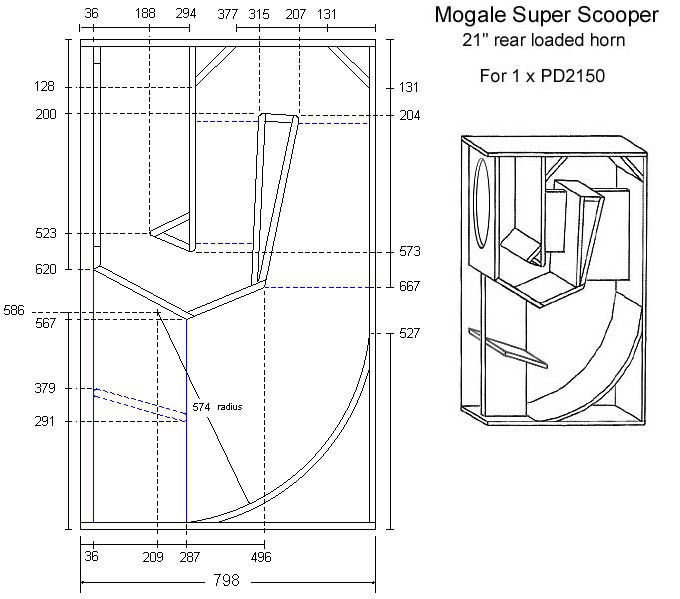
\includegraphics[scale=0.5]{./img/21MogaleSuperScooper.jpg}
    \caption{Vista de perfil del 21" \ Mogale Super Scooper}
    \label{fig:logoETSII}
\end{figure}

En la inmensa mayoría de casos el tamaño original de la imagen no se adapta correctamente a las dimensiones de la página, por lo que es necesario redimensionar la imagen mediante el argumento \texttt{scale} de \textbackslash\texttt{includegraphics}. 

Al igual que para las tablas, existen distintas alternativas en cuanto a su posicionamiento (que, se recuerda, pueden consultarse en \url{https://www.overleaf.com/learn/latex/positioning_images_and_tables}), el título se indica mediante el comando \textbackslash\texttt{caption} y la referencia mediante el comando \textbackslash\texttt{label}. 

Existen, además, diversas opciones en lo relativo al manejo de imágenes que no se detallan en este documento, pero que pueden consultarse en \url{https://es.overleaf.com/learn/latex/Inserting_Images} 

%%%%%%%%%%%%%%%%%%%%%%%%%%%%%%%%%%%%%%%%%%%%%%%%%%


%%%%%%%%%%%%%%%%% - ECUACIONES - %%%%%%%%%%%%%%%%%

\newpage
\section{ECUACIONES} \label{sec:ecuaciones}

Una de las mayores ventajas de \LaTeX \ es lo fácil y rápido que resulta incorporar ecuaciones en el documento. Las ecuaciones se definen en el entorno \texttt{equation}, mediante el cual la identidad de Euler, por ejemplo, quedaría como:

\begin{equation}
    e^{i\pi} + 1 = 0
    \label{eq:euler}
\end{equation}

o la serie de Leibniz:

\begin{equation}
    \sum_{n=0}^\infty \frac{(-1)^n}{2n+1} = \frac{\pi}{4}
    \label{eq:leibniz}
\end{equation}

Como se puede ver, las ecuaciones se numeran de forma automática con respecto al capítulo en el que se encuentran (para no numerar una ecuación basta con definir el entorno como \textbackslash\texttt{begin\{equation*\}}), número al que se puede hacer referencia definiendo el comando \textbackslash\texttt{label}.

En este apartado se utilizan algunos de los símbolos matemáticos básicos, para más información sobre los distintos comandos que corresponden a diversos símbolos puede consultarse \url{https://www.caam.rice.edu/~heinken/latex/symbols.pdf}.


\subsection{Ecuaciones en el texto}

También existe la posibilidad de introducir expresiones matemáticas en una línea de texto encerrando la expresión entre dos símbolos \$, mediante lo cual se puede hacer referencia al número complejo $i$, que puede definirse como $\sqrt{-1}=i$, sin necesidad de interrumpir la oración.


\subsection{Entorno \textbackslash\texttt{split}}

En el caso de que una ecuación sea demasiado larga como para caber en una única línea puede usarse el entorno \texttt{split}, utilizado para el desarrollo de la serie de Taylor de $\sin{x}$ que aparece a continuación:

\begin{equation}
\begin{split}
    \sin{x} = \ & x - \frac{x^3}{3!} + \frac{x^5}{5!} - \frac{x^7}{7!} + \frac{x^9}{9!} - \frac{x^{11}}{11!} + \frac{x^13}{13!} + \dots \\ & + (-1)^n \frac{x^{2n+1}}{(2n+1)!} + \dots \qquad , \forall x \in \mathbb{R}
    \label{eq:taylor}
\end{split}
\end{equation}

La disposición de la ecuación no se hace automáticamente, por lo que es necesario indicar en qué lugar quedan verticalmente alineadas las distintas líneas (esto se realiza mediante el símbolo \& que en este caso va colocado después del $=$ en la primera línea y antes del primer $+$ de la segunda línea) y en qué momento se salta a la línea (que se indica mediante el comando \textbackslash\textbackslash).


\subsection{La herramienta Mathpix}

Mathpix es una aplicación que permite traducir a lenguaje \LaTeX \ cualquier ecuación, ya se encuentre en un archivo PDF o escrita a mano en un folio de papel. Aunque el proceso de plasmar ecuaciones en un documento \LaTeX \ ya es sencillo y rápido, esta herramienta lo vuelve casi instantáneo. La aplicación puede descargarse desde la página web de Mathpix: \url{https://mathpix.com/}.

%%%%%%%%%%%%%%%%%%%%%%%%%%%%%%%%%%%%%%%%%%%%%%%%%%


%%%%%%%%%%%%%%%%%% - GRÁFICAS - %%%%%%%%%%%%%%%%%%

\newpage
\section{GRÁFICAS} \label{sec:graficas}

Existen principalmente dos formas de insertar gráficas en un documento \LaTeX: mediante un archivo \textit{.pgf} generado por un programa externo (mediante Python utilizando la librería matplotlib, por ejemplo), o haciendo uso del paquete TikZ.


\subsection{Gráficas PGF}

Insertar gráficas en formato PGF es muy sencillo, el procedimiento es esencialmente el mismo que al insertar una imagen (entorno \texttt{figure}), pero sustituyendo \textbackslash\texttt{includegraphics} por \textbackslash\texttt{input}, seguido del archivo \textit{.pgf} correspondiente. En este caso las dimensiones de la gráfica se ajustan mediante el comando \textbackslash\texttt{scalebox}. 

\begin{figure}[H]
    \centering
    \scalebox{1.1}{%% Creator: Matplotlib, PGF backend
%%
%% To include the figure in your LaTeX document, write
%%   \input{<filename>.pgf}
%%
%% Make sure the required packages are loaded in your preamble
%%   \usepackage{pgf}
%%
%% Figures using additional raster images can only be included by \input if
%% they are in the same directory as the main LaTeX file. For loading figures
%% from other directories you can use the `import` package
%%   \usepackage{import}
%% and then include the figures with
%%   \import{<path to file>}{<filename>.pgf}
%%
%% Matplotlib used the following preamble
%%
\begingroup%
\makeatletter%
\begin{pgfpicture}%
\pgfpathrectangle{\pgfpointorigin}{\pgfqpoint{6.000000in}{4.000000in}}%
\pgfusepath{use as bounding box, clip}%
\begin{pgfscope}%
\pgfsetbuttcap%
\pgfsetmiterjoin%
\definecolor{currentfill}{rgb}{1.000000,1.000000,1.000000}%
\pgfsetfillcolor{currentfill}%
\pgfsetlinewidth{0.000000pt}%
\definecolor{currentstroke}{rgb}{1.000000,1.000000,1.000000}%
\pgfsetstrokecolor{currentstroke}%
\pgfsetdash{}{0pt}%
\pgfpathmoveto{\pgfqpoint{0.000000in}{0.000000in}}%
\pgfpathlineto{\pgfqpoint{6.000000in}{0.000000in}}%
\pgfpathlineto{\pgfqpoint{6.000000in}{4.000000in}}%
\pgfpathlineto{\pgfqpoint{0.000000in}{4.000000in}}%
\pgfpathclose%
\pgfusepath{fill}%
\end{pgfscope}%
\begin{pgfscope}%
\pgfsetbuttcap%
\pgfsetmiterjoin%
\definecolor{currentfill}{rgb}{1.000000,1.000000,1.000000}%
\pgfsetfillcolor{currentfill}%
\pgfsetlinewidth{0.000000pt}%
\definecolor{currentstroke}{rgb}{0.000000,0.000000,0.000000}%
\pgfsetstrokecolor{currentstroke}%
\pgfsetstrokeopacity{0.000000}%
\pgfsetdash{}{0pt}%
\pgfpathmoveto{\pgfqpoint{0.750000in}{0.500000in}}%
\pgfpathlineto{\pgfqpoint{5.400000in}{0.500000in}}%
\pgfpathlineto{\pgfqpoint{5.400000in}{3.520000in}}%
\pgfpathlineto{\pgfqpoint{0.750000in}{3.520000in}}%
\pgfpathclose%
\pgfusepath{fill}%
\end{pgfscope}%
\begin{pgfscope}%
\pgfpathrectangle{\pgfqpoint{0.750000in}{0.500000in}}{\pgfqpoint{4.650000in}{3.020000in}}%
\pgfusepath{clip}%
\pgfsetrectcap%
\pgfsetroundjoin%
\pgfsetlinewidth{0.803000pt}%
\definecolor{currentstroke}{rgb}{0.690196,0.690196,0.690196}%
\pgfsetstrokecolor{currentstroke}%
\pgfsetdash{}{0pt}%
\pgfpathmoveto{\pgfqpoint{0.961364in}{0.500000in}}%
\pgfpathlineto{\pgfqpoint{0.961364in}{3.520000in}}%
\pgfusepath{stroke}%
\end{pgfscope}%
\begin{pgfscope}%
\pgfsetbuttcap%
\pgfsetroundjoin%
\definecolor{currentfill}{rgb}{0.000000,0.000000,0.000000}%
\pgfsetfillcolor{currentfill}%
\pgfsetlinewidth{0.803000pt}%
\definecolor{currentstroke}{rgb}{0.000000,0.000000,0.000000}%
\pgfsetstrokecolor{currentstroke}%
\pgfsetdash{}{0pt}%
\pgfsys@defobject{currentmarker}{\pgfqpoint{0.000000in}{-0.048611in}}{\pgfqpoint{0.000000in}{0.000000in}}{%
\pgfpathmoveto{\pgfqpoint{0.000000in}{0.000000in}}%
\pgfpathlineto{\pgfqpoint{0.000000in}{-0.048611in}}%
\pgfusepath{stroke,fill}%
}%
\begin{pgfscope}%
\pgfsys@transformshift{0.961364in}{0.500000in}%
\pgfsys@useobject{currentmarker}{}%
\end{pgfscope}%
\end{pgfscope}%
\begin{pgfscope}%
\definecolor{textcolor}{rgb}{0.000000,0.000000,0.000000}%
\pgfsetstrokecolor{textcolor}%
\pgfsetfillcolor{textcolor}%
\pgftext[x=0.961364in,y=0.402778in,,top]{\color{textcolor}\rmfamily\fontsize{10.000000}{12.000000}\selectfont \(\displaystyle 0\)}%
\end{pgfscope}%
\begin{pgfscope}%
\pgfpathrectangle{\pgfqpoint{0.750000in}{0.500000in}}{\pgfqpoint{4.650000in}{3.020000in}}%
\pgfusepath{clip}%
\pgfsetrectcap%
\pgfsetroundjoin%
\pgfsetlinewidth{0.803000pt}%
\definecolor{currentstroke}{rgb}{0.690196,0.690196,0.690196}%
\pgfsetstrokecolor{currentstroke}%
\pgfsetdash{}{0pt}%
\pgfpathmoveto{\pgfqpoint{1.665909in}{0.500000in}}%
\pgfpathlineto{\pgfqpoint{1.665909in}{3.520000in}}%
\pgfusepath{stroke}%
\end{pgfscope}%
\begin{pgfscope}%
\pgfsetbuttcap%
\pgfsetroundjoin%
\definecolor{currentfill}{rgb}{0.000000,0.000000,0.000000}%
\pgfsetfillcolor{currentfill}%
\pgfsetlinewidth{0.803000pt}%
\definecolor{currentstroke}{rgb}{0.000000,0.000000,0.000000}%
\pgfsetstrokecolor{currentstroke}%
\pgfsetdash{}{0pt}%
\pgfsys@defobject{currentmarker}{\pgfqpoint{0.000000in}{-0.048611in}}{\pgfqpoint{0.000000in}{0.000000in}}{%
\pgfpathmoveto{\pgfqpoint{0.000000in}{0.000000in}}%
\pgfpathlineto{\pgfqpoint{0.000000in}{-0.048611in}}%
\pgfusepath{stroke,fill}%
}%
\begin{pgfscope}%
\pgfsys@transformshift{1.665909in}{0.500000in}%
\pgfsys@useobject{currentmarker}{}%
\end{pgfscope}%
\end{pgfscope}%
\begin{pgfscope}%
\definecolor{textcolor}{rgb}{0.000000,0.000000,0.000000}%
\pgfsetstrokecolor{textcolor}%
\pgfsetfillcolor{textcolor}%
\pgftext[x=1.665909in,y=0.402778in,,top]{\color{textcolor}\rmfamily\fontsize{10.000000}{12.000000}\selectfont \(\displaystyle 1\)}%
\end{pgfscope}%
\begin{pgfscope}%
\pgfpathrectangle{\pgfqpoint{0.750000in}{0.500000in}}{\pgfqpoint{4.650000in}{3.020000in}}%
\pgfusepath{clip}%
\pgfsetrectcap%
\pgfsetroundjoin%
\pgfsetlinewidth{0.803000pt}%
\definecolor{currentstroke}{rgb}{0.690196,0.690196,0.690196}%
\pgfsetstrokecolor{currentstroke}%
\pgfsetdash{}{0pt}%
\pgfpathmoveto{\pgfqpoint{2.370455in}{0.500000in}}%
\pgfpathlineto{\pgfqpoint{2.370455in}{3.520000in}}%
\pgfusepath{stroke}%
\end{pgfscope}%
\begin{pgfscope}%
\pgfsetbuttcap%
\pgfsetroundjoin%
\definecolor{currentfill}{rgb}{0.000000,0.000000,0.000000}%
\pgfsetfillcolor{currentfill}%
\pgfsetlinewidth{0.803000pt}%
\definecolor{currentstroke}{rgb}{0.000000,0.000000,0.000000}%
\pgfsetstrokecolor{currentstroke}%
\pgfsetdash{}{0pt}%
\pgfsys@defobject{currentmarker}{\pgfqpoint{0.000000in}{-0.048611in}}{\pgfqpoint{0.000000in}{0.000000in}}{%
\pgfpathmoveto{\pgfqpoint{0.000000in}{0.000000in}}%
\pgfpathlineto{\pgfqpoint{0.000000in}{-0.048611in}}%
\pgfusepath{stroke,fill}%
}%
\begin{pgfscope}%
\pgfsys@transformshift{2.370455in}{0.500000in}%
\pgfsys@useobject{currentmarker}{}%
\end{pgfscope}%
\end{pgfscope}%
\begin{pgfscope}%
\definecolor{textcolor}{rgb}{0.000000,0.000000,0.000000}%
\pgfsetstrokecolor{textcolor}%
\pgfsetfillcolor{textcolor}%
\pgftext[x=2.370455in,y=0.402778in,,top]{\color{textcolor}\rmfamily\fontsize{10.000000}{12.000000}\selectfont \(\displaystyle 2\)}%
\end{pgfscope}%
\begin{pgfscope}%
\pgfpathrectangle{\pgfqpoint{0.750000in}{0.500000in}}{\pgfqpoint{4.650000in}{3.020000in}}%
\pgfusepath{clip}%
\pgfsetrectcap%
\pgfsetroundjoin%
\pgfsetlinewidth{0.803000pt}%
\definecolor{currentstroke}{rgb}{0.690196,0.690196,0.690196}%
\pgfsetstrokecolor{currentstroke}%
\pgfsetdash{}{0pt}%
\pgfpathmoveto{\pgfqpoint{3.075000in}{0.500000in}}%
\pgfpathlineto{\pgfqpoint{3.075000in}{3.520000in}}%
\pgfusepath{stroke}%
\end{pgfscope}%
\begin{pgfscope}%
\pgfsetbuttcap%
\pgfsetroundjoin%
\definecolor{currentfill}{rgb}{0.000000,0.000000,0.000000}%
\pgfsetfillcolor{currentfill}%
\pgfsetlinewidth{0.803000pt}%
\definecolor{currentstroke}{rgb}{0.000000,0.000000,0.000000}%
\pgfsetstrokecolor{currentstroke}%
\pgfsetdash{}{0pt}%
\pgfsys@defobject{currentmarker}{\pgfqpoint{0.000000in}{-0.048611in}}{\pgfqpoint{0.000000in}{0.000000in}}{%
\pgfpathmoveto{\pgfqpoint{0.000000in}{0.000000in}}%
\pgfpathlineto{\pgfqpoint{0.000000in}{-0.048611in}}%
\pgfusepath{stroke,fill}%
}%
\begin{pgfscope}%
\pgfsys@transformshift{3.075000in}{0.500000in}%
\pgfsys@useobject{currentmarker}{}%
\end{pgfscope}%
\end{pgfscope}%
\begin{pgfscope}%
\definecolor{textcolor}{rgb}{0.000000,0.000000,0.000000}%
\pgfsetstrokecolor{textcolor}%
\pgfsetfillcolor{textcolor}%
\pgftext[x=3.075000in,y=0.402778in,,top]{\color{textcolor}\rmfamily\fontsize{10.000000}{12.000000}\selectfont \(\displaystyle 3\)}%
\end{pgfscope}%
\begin{pgfscope}%
\pgfpathrectangle{\pgfqpoint{0.750000in}{0.500000in}}{\pgfqpoint{4.650000in}{3.020000in}}%
\pgfusepath{clip}%
\pgfsetrectcap%
\pgfsetroundjoin%
\pgfsetlinewidth{0.803000pt}%
\definecolor{currentstroke}{rgb}{0.690196,0.690196,0.690196}%
\pgfsetstrokecolor{currentstroke}%
\pgfsetdash{}{0pt}%
\pgfpathmoveto{\pgfqpoint{3.779545in}{0.500000in}}%
\pgfpathlineto{\pgfqpoint{3.779545in}{3.520000in}}%
\pgfusepath{stroke}%
\end{pgfscope}%
\begin{pgfscope}%
\pgfsetbuttcap%
\pgfsetroundjoin%
\definecolor{currentfill}{rgb}{0.000000,0.000000,0.000000}%
\pgfsetfillcolor{currentfill}%
\pgfsetlinewidth{0.803000pt}%
\definecolor{currentstroke}{rgb}{0.000000,0.000000,0.000000}%
\pgfsetstrokecolor{currentstroke}%
\pgfsetdash{}{0pt}%
\pgfsys@defobject{currentmarker}{\pgfqpoint{0.000000in}{-0.048611in}}{\pgfqpoint{0.000000in}{0.000000in}}{%
\pgfpathmoveto{\pgfqpoint{0.000000in}{0.000000in}}%
\pgfpathlineto{\pgfqpoint{0.000000in}{-0.048611in}}%
\pgfusepath{stroke,fill}%
}%
\begin{pgfscope}%
\pgfsys@transformshift{3.779545in}{0.500000in}%
\pgfsys@useobject{currentmarker}{}%
\end{pgfscope}%
\end{pgfscope}%
\begin{pgfscope}%
\definecolor{textcolor}{rgb}{0.000000,0.000000,0.000000}%
\pgfsetstrokecolor{textcolor}%
\pgfsetfillcolor{textcolor}%
\pgftext[x=3.779545in,y=0.402778in,,top]{\color{textcolor}\rmfamily\fontsize{10.000000}{12.000000}\selectfont \(\displaystyle 4\)}%
\end{pgfscope}%
\begin{pgfscope}%
\pgfpathrectangle{\pgfqpoint{0.750000in}{0.500000in}}{\pgfqpoint{4.650000in}{3.020000in}}%
\pgfusepath{clip}%
\pgfsetrectcap%
\pgfsetroundjoin%
\pgfsetlinewidth{0.803000pt}%
\definecolor{currentstroke}{rgb}{0.690196,0.690196,0.690196}%
\pgfsetstrokecolor{currentstroke}%
\pgfsetdash{}{0pt}%
\pgfpathmoveto{\pgfqpoint{4.484091in}{0.500000in}}%
\pgfpathlineto{\pgfqpoint{4.484091in}{3.520000in}}%
\pgfusepath{stroke}%
\end{pgfscope}%
\begin{pgfscope}%
\pgfsetbuttcap%
\pgfsetroundjoin%
\definecolor{currentfill}{rgb}{0.000000,0.000000,0.000000}%
\pgfsetfillcolor{currentfill}%
\pgfsetlinewidth{0.803000pt}%
\definecolor{currentstroke}{rgb}{0.000000,0.000000,0.000000}%
\pgfsetstrokecolor{currentstroke}%
\pgfsetdash{}{0pt}%
\pgfsys@defobject{currentmarker}{\pgfqpoint{0.000000in}{-0.048611in}}{\pgfqpoint{0.000000in}{0.000000in}}{%
\pgfpathmoveto{\pgfqpoint{0.000000in}{0.000000in}}%
\pgfpathlineto{\pgfqpoint{0.000000in}{-0.048611in}}%
\pgfusepath{stroke,fill}%
}%
\begin{pgfscope}%
\pgfsys@transformshift{4.484091in}{0.500000in}%
\pgfsys@useobject{currentmarker}{}%
\end{pgfscope}%
\end{pgfscope}%
\begin{pgfscope}%
\definecolor{textcolor}{rgb}{0.000000,0.000000,0.000000}%
\pgfsetstrokecolor{textcolor}%
\pgfsetfillcolor{textcolor}%
\pgftext[x=4.484091in,y=0.402778in,,top]{\color{textcolor}\rmfamily\fontsize{10.000000}{12.000000}\selectfont \(\displaystyle 5\)}%
\end{pgfscope}%
\begin{pgfscope}%
\pgfpathrectangle{\pgfqpoint{0.750000in}{0.500000in}}{\pgfqpoint{4.650000in}{3.020000in}}%
\pgfusepath{clip}%
\pgfsetrectcap%
\pgfsetroundjoin%
\pgfsetlinewidth{0.803000pt}%
\definecolor{currentstroke}{rgb}{0.690196,0.690196,0.690196}%
\pgfsetstrokecolor{currentstroke}%
\pgfsetdash{}{0pt}%
\pgfpathmoveto{\pgfqpoint{5.188636in}{0.500000in}}%
\pgfpathlineto{\pgfqpoint{5.188636in}{3.520000in}}%
\pgfusepath{stroke}%
\end{pgfscope}%
\begin{pgfscope}%
\pgfsetbuttcap%
\pgfsetroundjoin%
\definecolor{currentfill}{rgb}{0.000000,0.000000,0.000000}%
\pgfsetfillcolor{currentfill}%
\pgfsetlinewidth{0.803000pt}%
\definecolor{currentstroke}{rgb}{0.000000,0.000000,0.000000}%
\pgfsetstrokecolor{currentstroke}%
\pgfsetdash{}{0pt}%
\pgfsys@defobject{currentmarker}{\pgfqpoint{0.000000in}{-0.048611in}}{\pgfqpoint{0.000000in}{0.000000in}}{%
\pgfpathmoveto{\pgfqpoint{0.000000in}{0.000000in}}%
\pgfpathlineto{\pgfqpoint{0.000000in}{-0.048611in}}%
\pgfusepath{stroke,fill}%
}%
\begin{pgfscope}%
\pgfsys@transformshift{5.188636in}{0.500000in}%
\pgfsys@useobject{currentmarker}{}%
\end{pgfscope}%
\end{pgfscope}%
\begin{pgfscope}%
\definecolor{textcolor}{rgb}{0.000000,0.000000,0.000000}%
\pgfsetstrokecolor{textcolor}%
\pgfsetfillcolor{textcolor}%
\pgftext[x=5.188636in,y=0.402778in,,top]{\color{textcolor}\rmfamily\fontsize{10.000000}{12.000000}\selectfont \(\displaystyle 6\)}%
\end{pgfscope}%
\begin{pgfscope}%
\definecolor{textcolor}{rgb}{0.000000,0.000000,0.000000}%
\pgfsetstrokecolor{textcolor}%
\pgfsetfillcolor{textcolor}%
\pgftext[x=3.075000in,y=0.223766in,,top]{\color{textcolor}\rmfamily\fontsize{10.000000}{12.000000}\selectfont Tiempo}%
\end{pgfscope}%
\begin{pgfscope}%
\pgfpathrectangle{\pgfqpoint{0.750000in}{0.500000in}}{\pgfqpoint{4.650000in}{3.020000in}}%
\pgfusepath{clip}%
\pgfsetrectcap%
\pgfsetroundjoin%
\pgfsetlinewidth{0.803000pt}%
\definecolor{currentstroke}{rgb}{0.690196,0.690196,0.690196}%
\pgfsetstrokecolor{currentstroke}%
\pgfsetdash{}{0pt}%
\pgfpathmoveto{\pgfqpoint{0.750000in}{0.500000in}}%
\pgfpathlineto{\pgfqpoint{5.400000in}{0.500000in}}%
\pgfusepath{stroke}%
\end{pgfscope}%
\begin{pgfscope}%
\pgfsetbuttcap%
\pgfsetroundjoin%
\definecolor{currentfill}{rgb}{0.000000,0.000000,0.000000}%
\pgfsetfillcolor{currentfill}%
\pgfsetlinewidth{0.803000pt}%
\definecolor{currentstroke}{rgb}{0.000000,0.000000,0.000000}%
\pgfsetstrokecolor{currentstroke}%
\pgfsetdash{}{0pt}%
\pgfsys@defobject{currentmarker}{\pgfqpoint{-0.048611in}{0.000000in}}{\pgfqpoint{0.000000in}{0.000000in}}{%
\pgfpathmoveto{\pgfqpoint{0.000000in}{0.000000in}}%
\pgfpathlineto{\pgfqpoint{-0.048611in}{0.000000in}}%
\pgfusepath{stroke,fill}%
}%
\begin{pgfscope}%
\pgfsys@transformshift{0.750000in}{0.500000in}%
\pgfsys@useobject{currentmarker}{}%
\end{pgfscope}%
\end{pgfscope}%
\begin{pgfscope}%
\definecolor{textcolor}{rgb}{0.000000,0.000000,0.000000}%
\pgfsetstrokecolor{textcolor}%
\pgfsetfillcolor{textcolor}%
\pgftext[x=0.475308in,y=0.451775in,left,base]{\color{textcolor}\rmfamily\fontsize{10.000000}{12.000000}\selectfont \(\displaystyle -3\)}%
\end{pgfscope}%
\begin{pgfscope}%
\pgfpathrectangle{\pgfqpoint{0.750000in}{0.500000in}}{\pgfqpoint{4.650000in}{3.020000in}}%
\pgfusepath{clip}%
\pgfsetrectcap%
\pgfsetroundjoin%
\pgfsetlinewidth{0.803000pt}%
\definecolor{currentstroke}{rgb}{0.690196,0.690196,0.690196}%
\pgfsetstrokecolor{currentstroke}%
\pgfsetdash{}{0pt}%
\pgfpathmoveto{\pgfqpoint{0.750000in}{1.003333in}}%
\pgfpathlineto{\pgfqpoint{5.400000in}{1.003333in}}%
\pgfusepath{stroke}%
\end{pgfscope}%
\begin{pgfscope}%
\pgfsetbuttcap%
\pgfsetroundjoin%
\definecolor{currentfill}{rgb}{0.000000,0.000000,0.000000}%
\pgfsetfillcolor{currentfill}%
\pgfsetlinewidth{0.803000pt}%
\definecolor{currentstroke}{rgb}{0.000000,0.000000,0.000000}%
\pgfsetstrokecolor{currentstroke}%
\pgfsetdash{}{0pt}%
\pgfsys@defobject{currentmarker}{\pgfqpoint{-0.048611in}{0.000000in}}{\pgfqpoint{0.000000in}{0.000000in}}{%
\pgfpathmoveto{\pgfqpoint{0.000000in}{0.000000in}}%
\pgfpathlineto{\pgfqpoint{-0.048611in}{0.000000in}}%
\pgfusepath{stroke,fill}%
}%
\begin{pgfscope}%
\pgfsys@transformshift{0.750000in}{1.003333in}%
\pgfsys@useobject{currentmarker}{}%
\end{pgfscope}%
\end{pgfscope}%
\begin{pgfscope}%
\definecolor{textcolor}{rgb}{0.000000,0.000000,0.000000}%
\pgfsetstrokecolor{textcolor}%
\pgfsetfillcolor{textcolor}%
\pgftext[x=0.475308in,y=0.955108in,left,base]{\color{textcolor}\rmfamily\fontsize{10.000000}{12.000000}\selectfont \(\displaystyle -2\)}%
\end{pgfscope}%
\begin{pgfscope}%
\pgfpathrectangle{\pgfqpoint{0.750000in}{0.500000in}}{\pgfqpoint{4.650000in}{3.020000in}}%
\pgfusepath{clip}%
\pgfsetrectcap%
\pgfsetroundjoin%
\pgfsetlinewidth{0.803000pt}%
\definecolor{currentstroke}{rgb}{0.690196,0.690196,0.690196}%
\pgfsetstrokecolor{currentstroke}%
\pgfsetdash{}{0pt}%
\pgfpathmoveto{\pgfqpoint{0.750000in}{1.506667in}}%
\pgfpathlineto{\pgfqpoint{5.400000in}{1.506667in}}%
\pgfusepath{stroke}%
\end{pgfscope}%
\begin{pgfscope}%
\pgfsetbuttcap%
\pgfsetroundjoin%
\definecolor{currentfill}{rgb}{0.000000,0.000000,0.000000}%
\pgfsetfillcolor{currentfill}%
\pgfsetlinewidth{0.803000pt}%
\definecolor{currentstroke}{rgb}{0.000000,0.000000,0.000000}%
\pgfsetstrokecolor{currentstroke}%
\pgfsetdash{}{0pt}%
\pgfsys@defobject{currentmarker}{\pgfqpoint{-0.048611in}{0.000000in}}{\pgfqpoint{0.000000in}{0.000000in}}{%
\pgfpathmoveto{\pgfqpoint{0.000000in}{0.000000in}}%
\pgfpathlineto{\pgfqpoint{-0.048611in}{0.000000in}}%
\pgfusepath{stroke,fill}%
}%
\begin{pgfscope}%
\pgfsys@transformshift{0.750000in}{1.506667in}%
\pgfsys@useobject{currentmarker}{}%
\end{pgfscope}%
\end{pgfscope}%
\begin{pgfscope}%
\definecolor{textcolor}{rgb}{0.000000,0.000000,0.000000}%
\pgfsetstrokecolor{textcolor}%
\pgfsetfillcolor{textcolor}%
\pgftext[x=0.475308in,y=1.458441in,left,base]{\color{textcolor}\rmfamily\fontsize{10.000000}{12.000000}\selectfont \(\displaystyle -1\)}%
\end{pgfscope}%
\begin{pgfscope}%
\pgfpathrectangle{\pgfqpoint{0.750000in}{0.500000in}}{\pgfqpoint{4.650000in}{3.020000in}}%
\pgfusepath{clip}%
\pgfsetrectcap%
\pgfsetroundjoin%
\pgfsetlinewidth{0.803000pt}%
\definecolor{currentstroke}{rgb}{0.690196,0.690196,0.690196}%
\pgfsetstrokecolor{currentstroke}%
\pgfsetdash{}{0pt}%
\pgfpathmoveto{\pgfqpoint{0.750000in}{2.010000in}}%
\pgfpathlineto{\pgfqpoint{5.400000in}{2.010000in}}%
\pgfusepath{stroke}%
\end{pgfscope}%
\begin{pgfscope}%
\pgfsetbuttcap%
\pgfsetroundjoin%
\definecolor{currentfill}{rgb}{0.000000,0.000000,0.000000}%
\pgfsetfillcolor{currentfill}%
\pgfsetlinewidth{0.803000pt}%
\definecolor{currentstroke}{rgb}{0.000000,0.000000,0.000000}%
\pgfsetstrokecolor{currentstroke}%
\pgfsetdash{}{0pt}%
\pgfsys@defobject{currentmarker}{\pgfqpoint{-0.048611in}{0.000000in}}{\pgfqpoint{0.000000in}{0.000000in}}{%
\pgfpathmoveto{\pgfqpoint{0.000000in}{0.000000in}}%
\pgfpathlineto{\pgfqpoint{-0.048611in}{0.000000in}}%
\pgfusepath{stroke,fill}%
}%
\begin{pgfscope}%
\pgfsys@transformshift{0.750000in}{2.010000in}%
\pgfsys@useobject{currentmarker}{}%
\end{pgfscope}%
\end{pgfscope}%
\begin{pgfscope}%
\definecolor{textcolor}{rgb}{0.000000,0.000000,0.000000}%
\pgfsetstrokecolor{textcolor}%
\pgfsetfillcolor{textcolor}%
\pgftext[x=0.583333in,y=1.961775in,left,base]{\color{textcolor}\rmfamily\fontsize{10.000000}{12.000000}\selectfont \(\displaystyle 0\)}%
\end{pgfscope}%
\begin{pgfscope}%
\pgfpathrectangle{\pgfqpoint{0.750000in}{0.500000in}}{\pgfqpoint{4.650000in}{3.020000in}}%
\pgfusepath{clip}%
\pgfsetrectcap%
\pgfsetroundjoin%
\pgfsetlinewidth{0.803000pt}%
\definecolor{currentstroke}{rgb}{0.690196,0.690196,0.690196}%
\pgfsetstrokecolor{currentstroke}%
\pgfsetdash{}{0pt}%
\pgfpathmoveto{\pgfqpoint{0.750000in}{2.513333in}}%
\pgfpathlineto{\pgfqpoint{5.400000in}{2.513333in}}%
\pgfusepath{stroke}%
\end{pgfscope}%
\begin{pgfscope}%
\pgfsetbuttcap%
\pgfsetroundjoin%
\definecolor{currentfill}{rgb}{0.000000,0.000000,0.000000}%
\pgfsetfillcolor{currentfill}%
\pgfsetlinewidth{0.803000pt}%
\definecolor{currentstroke}{rgb}{0.000000,0.000000,0.000000}%
\pgfsetstrokecolor{currentstroke}%
\pgfsetdash{}{0pt}%
\pgfsys@defobject{currentmarker}{\pgfqpoint{-0.048611in}{0.000000in}}{\pgfqpoint{0.000000in}{0.000000in}}{%
\pgfpathmoveto{\pgfqpoint{0.000000in}{0.000000in}}%
\pgfpathlineto{\pgfqpoint{-0.048611in}{0.000000in}}%
\pgfusepath{stroke,fill}%
}%
\begin{pgfscope}%
\pgfsys@transformshift{0.750000in}{2.513333in}%
\pgfsys@useobject{currentmarker}{}%
\end{pgfscope}%
\end{pgfscope}%
\begin{pgfscope}%
\definecolor{textcolor}{rgb}{0.000000,0.000000,0.000000}%
\pgfsetstrokecolor{textcolor}%
\pgfsetfillcolor{textcolor}%
\pgftext[x=0.583333in,y=2.465108in,left,base]{\color{textcolor}\rmfamily\fontsize{10.000000}{12.000000}\selectfont \(\displaystyle 1\)}%
\end{pgfscope}%
\begin{pgfscope}%
\pgfpathrectangle{\pgfqpoint{0.750000in}{0.500000in}}{\pgfqpoint{4.650000in}{3.020000in}}%
\pgfusepath{clip}%
\pgfsetrectcap%
\pgfsetroundjoin%
\pgfsetlinewidth{0.803000pt}%
\definecolor{currentstroke}{rgb}{0.690196,0.690196,0.690196}%
\pgfsetstrokecolor{currentstroke}%
\pgfsetdash{}{0pt}%
\pgfpathmoveto{\pgfqpoint{0.750000in}{3.016667in}}%
\pgfpathlineto{\pgfqpoint{5.400000in}{3.016667in}}%
\pgfusepath{stroke}%
\end{pgfscope}%
\begin{pgfscope}%
\pgfsetbuttcap%
\pgfsetroundjoin%
\definecolor{currentfill}{rgb}{0.000000,0.000000,0.000000}%
\pgfsetfillcolor{currentfill}%
\pgfsetlinewidth{0.803000pt}%
\definecolor{currentstroke}{rgb}{0.000000,0.000000,0.000000}%
\pgfsetstrokecolor{currentstroke}%
\pgfsetdash{}{0pt}%
\pgfsys@defobject{currentmarker}{\pgfqpoint{-0.048611in}{0.000000in}}{\pgfqpoint{0.000000in}{0.000000in}}{%
\pgfpathmoveto{\pgfqpoint{0.000000in}{0.000000in}}%
\pgfpathlineto{\pgfqpoint{-0.048611in}{0.000000in}}%
\pgfusepath{stroke,fill}%
}%
\begin{pgfscope}%
\pgfsys@transformshift{0.750000in}{3.016667in}%
\pgfsys@useobject{currentmarker}{}%
\end{pgfscope}%
\end{pgfscope}%
\begin{pgfscope}%
\definecolor{textcolor}{rgb}{0.000000,0.000000,0.000000}%
\pgfsetstrokecolor{textcolor}%
\pgfsetfillcolor{textcolor}%
\pgftext[x=0.583333in,y=2.968441in,left,base]{\color{textcolor}\rmfamily\fontsize{10.000000}{12.000000}\selectfont \(\displaystyle 2\)}%
\end{pgfscope}%
\begin{pgfscope}%
\pgfpathrectangle{\pgfqpoint{0.750000in}{0.500000in}}{\pgfqpoint{4.650000in}{3.020000in}}%
\pgfusepath{clip}%
\pgfsetrectcap%
\pgfsetroundjoin%
\pgfsetlinewidth{0.803000pt}%
\definecolor{currentstroke}{rgb}{0.690196,0.690196,0.690196}%
\pgfsetstrokecolor{currentstroke}%
\pgfsetdash{}{0pt}%
\pgfpathmoveto{\pgfqpoint{0.750000in}{3.520000in}}%
\pgfpathlineto{\pgfqpoint{5.400000in}{3.520000in}}%
\pgfusepath{stroke}%
\end{pgfscope}%
\begin{pgfscope}%
\pgfsetbuttcap%
\pgfsetroundjoin%
\definecolor{currentfill}{rgb}{0.000000,0.000000,0.000000}%
\pgfsetfillcolor{currentfill}%
\pgfsetlinewidth{0.803000pt}%
\definecolor{currentstroke}{rgb}{0.000000,0.000000,0.000000}%
\pgfsetstrokecolor{currentstroke}%
\pgfsetdash{}{0pt}%
\pgfsys@defobject{currentmarker}{\pgfqpoint{-0.048611in}{0.000000in}}{\pgfqpoint{0.000000in}{0.000000in}}{%
\pgfpathmoveto{\pgfqpoint{0.000000in}{0.000000in}}%
\pgfpathlineto{\pgfqpoint{-0.048611in}{0.000000in}}%
\pgfusepath{stroke,fill}%
}%
\begin{pgfscope}%
\pgfsys@transformshift{0.750000in}{3.520000in}%
\pgfsys@useobject{currentmarker}{}%
\end{pgfscope}%
\end{pgfscope}%
\begin{pgfscope}%
\definecolor{textcolor}{rgb}{0.000000,0.000000,0.000000}%
\pgfsetstrokecolor{textcolor}%
\pgfsetfillcolor{textcolor}%
\pgftext[x=0.583333in,y=3.471775in,left,base]{\color{textcolor}\rmfamily\fontsize{10.000000}{12.000000}\selectfont \(\displaystyle 3\)}%
\end{pgfscope}%
\begin{pgfscope}%
\definecolor{textcolor}{rgb}{0.000000,0.000000,0.000000}%
\pgfsetstrokecolor{textcolor}%
\pgfsetfillcolor{textcolor}%
\pgftext[x=0.419752in,y=2.010000in,,bottom,rotate=90.000000]{\color{textcolor}\rmfamily\fontsize{10.000000}{12.000000}\selectfont Amplitud}%
\end{pgfscope}%
\begin{pgfscope}%
\pgfpathrectangle{\pgfqpoint{0.750000in}{0.500000in}}{\pgfqpoint{4.650000in}{3.020000in}}%
\pgfusepath{clip}%
\pgfsetrectcap%
\pgfsetroundjoin%
\pgfsetlinewidth{0.501875pt}%
\definecolor{currentstroke}{rgb}{0.501961,0.501961,0.501961}%
\pgfsetstrokecolor{currentstroke}%
\pgfsetdash{}{0pt}%
\pgfpathmoveto{\pgfqpoint{0.961364in}{2.010000in}}%
\pgfpathlineto{\pgfqpoint{1.037531in}{2.436995in}}%
\pgfpathlineto{\pgfqpoint{1.079846in}{2.656093in}}%
\pgfpathlineto{\pgfqpoint{1.113698in}{2.815207in}}%
\pgfpathlineto{\pgfqpoint{1.143318in}{2.939524in}}%
\pgfpathlineto{\pgfqpoint{1.168707in}{3.033269in}}%
\pgfpathlineto{\pgfqpoint{1.189865in}{3.101429in}}%
\pgfpathlineto{\pgfqpoint{1.211022in}{3.159881in}}%
\pgfpathlineto{\pgfqpoint{1.227948in}{3.199301in}}%
\pgfpathlineto{\pgfqpoint{1.244874in}{3.231950in}}%
\pgfpathlineto{\pgfqpoint{1.261800in}{3.257642in}}%
\pgfpathlineto{\pgfqpoint{1.274495in}{3.272255in}}%
\pgfpathlineto{\pgfqpoint{1.287189in}{3.282826in}}%
\pgfpathlineto{\pgfqpoint{1.299884in}{3.289319in}}%
\pgfpathlineto{\pgfqpoint{1.312578in}{3.291714in}}%
\pgfpathlineto{\pgfqpoint{1.325273in}{3.290003in}}%
\pgfpathlineto{\pgfqpoint{1.337968in}{3.284192in}}%
\pgfpathlineto{\pgfqpoint{1.350662in}{3.274299in}}%
\pgfpathlineto{\pgfqpoint{1.363357in}{3.260356in}}%
\pgfpathlineto{\pgfqpoint{1.376051in}{3.242409in}}%
\pgfpathlineto{\pgfqpoint{1.392977in}{3.212349in}}%
\pgfpathlineto{\pgfqpoint{1.409903in}{3.175444in}}%
\pgfpathlineto{\pgfqpoint{1.426829in}{3.131903in}}%
\pgfpathlineto{\pgfqpoint{1.447987in}{3.068526in}}%
\pgfpathlineto{\pgfqpoint{1.469144in}{2.995736in}}%
\pgfpathlineto{\pgfqpoint{1.494533in}{2.896877in}}%
\pgfpathlineto{\pgfqpoint{1.524154in}{2.767288in}}%
\pgfpathlineto{\pgfqpoint{1.558006in}{2.603176in}}%
\pgfpathlineto{\pgfqpoint{1.596089in}{2.402624in}}%
\pgfpathlineto{\pgfqpoint{1.651099in}{2.094583in}}%
\pgfpathlineto{\pgfqpoint{1.744192in}{1.571623in}}%
\pgfpathlineto{\pgfqpoint{1.786507in}{1.353493in}}%
\pgfpathlineto{\pgfqpoint{1.820359in}{1.195421in}}%
\pgfpathlineto{\pgfqpoint{1.849980in}{1.072191in}}%
\pgfpathlineto{\pgfqpoint{1.875369in}{0.979495in}}%
\pgfpathlineto{\pgfqpoint{1.896526in}{0.912280in}}%
\pgfpathlineto{\pgfqpoint{1.917684in}{0.854829in}}%
\pgfpathlineto{\pgfqpoint{1.934610in}{0.816243in}}%
\pgfpathlineto{\pgfqpoint{1.951536in}{0.784455in}}%
\pgfpathlineto{\pgfqpoint{1.968462in}{0.759644in}}%
\pgfpathlineto{\pgfqpoint{1.981156in}{0.745701in}}%
\pgfpathlineto{\pgfqpoint{1.993851in}{0.735808in}}%
\pgfpathlineto{\pgfqpoint{2.006545in}{0.729997in}}%
\pgfpathlineto{\pgfqpoint{2.019240in}{0.728286in}}%
\pgfpathlineto{\pgfqpoint{2.031934in}{0.730681in}}%
\pgfpathlineto{\pgfqpoint{2.044629in}{0.737174in}}%
\pgfpathlineto{\pgfqpoint{2.057323in}{0.747745in}}%
\pgfpathlineto{\pgfqpoint{2.070018in}{0.762358in}}%
\pgfpathlineto{\pgfqpoint{2.082712in}{0.780968in}}%
\pgfpathlineto{\pgfqpoint{2.099638in}{0.811894in}}%
\pgfpathlineto{\pgfqpoint{2.116564in}{0.849641in}}%
\pgfpathlineto{\pgfqpoint{2.137722in}{0.906087in}}%
\pgfpathlineto{\pgfqpoint{2.158879in}{0.972350in}}%
\pgfpathlineto{\pgfqpoint{2.184268in}{1.063991in}}%
\pgfpathlineto{\pgfqpoint{2.209657in}{1.167743in}}%
\pgfpathlineto{\pgfqpoint{2.239278in}{1.302315in}}%
\pgfpathlineto{\pgfqpoint{2.273130in}{1.471060in}}%
\pgfpathlineto{\pgfqpoint{2.315445in}{1.698749in}}%
\pgfpathlineto{\pgfqpoint{2.387381in}{2.106645in}}%
\pgfpathlineto{\pgfqpoint{2.450853in}{2.459720in}}%
\pgfpathlineto{\pgfqpoint{2.488937in}{2.656093in}}%
\pgfpathlineto{\pgfqpoint{2.522789in}{2.815207in}}%
\pgfpathlineto{\pgfqpoint{2.552409in}{2.939524in}}%
\pgfpathlineto{\pgfqpoint{2.577798in}{3.033269in}}%
\pgfpathlineto{\pgfqpoint{2.598956in}{3.101429in}}%
\pgfpathlineto{\pgfqpoint{2.620113in}{3.159881in}}%
\pgfpathlineto{\pgfqpoint{2.637039in}{3.199301in}}%
\pgfpathlineto{\pgfqpoint{2.653965in}{3.231950in}}%
\pgfpathlineto{\pgfqpoint{2.670891in}{3.257642in}}%
\pgfpathlineto{\pgfqpoint{2.683586in}{3.272255in}}%
\pgfpathlineto{\pgfqpoint{2.696280in}{3.282826in}}%
\pgfpathlineto{\pgfqpoint{2.708975in}{3.289319in}}%
\pgfpathlineto{\pgfqpoint{2.721669in}{3.291714in}}%
\pgfpathlineto{\pgfqpoint{2.734364in}{3.290003in}}%
\pgfpathlineto{\pgfqpoint{2.747058in}{3.284192in}}%
\pgfpathlineto{\pgfqpoint{2.759753in}{3.274299in}}%
\pgfpathlineto{\pgfqpoint{2.772447in}{3.260356in}}%
\pgfpathlineto{\pgfqpoint{2.785142in}{3.242409in}}%
\pgfpathlineto{\pgfqpoint{2.802068in}{3.212349in}}%
\pgfpathlineto{\pgfqpoint{2.818994in}{3.175444in}}%
\pgfpathlineto{\pgfqpoint{2.835920in}{3.131903in}}%
\pgfpathlineto{\pgfqpoint{2.857078in}{3.068526in}}%
\pgfpathlineto{\pgfqpoint{2.878235in}{2.995736in}}%
\pgfpathlineto{\pgfqpoint{2.903624in}{2.896877in}}%
\pgfpathlineto{\pgfqpoint{2.933245in}{2.767288in}}%
\pgfpathlineto{\pgfqpoint{2.967097in}{2.603176in}}%
\pgfpathlineto{\pgfqpoint{3.005180in}{2.402624in}}%
\pgfpathlineto{\pgfqpoint{3.060190in}{2.094583in}}%
\pgfpathlineto{\pgfqpoint{3.153283in}{1.571623in}}%
\pgfpathlineto{\pgfqpoint{3.195598in}{1.353493in}}%
\pgfpathlineto{\pgfqpoint{3.229450in}{1.195421in}}%
\pgfpathlineto{\pgfqpoint{3.259070in}{1.072191in}}%
\pgfpathlineto{\pgfqpoint{3.284459in}{0.979495in}}%
\pgfpathlineto{\pgfqpoint{3.305617in}{0.912280in}}%
\pgfpathlineto{\pgfqpoint{3.326775in}{0.854829in}}%
\pgfpathlineto{\pgfqpoint{3.343701in}{0.816243in}}%
\pgfpathlineto{\pgfqpoint{3.360627in}{0.784455in}}%
\pgfpathlineto{\pgfqpoint{3.377553in}{0.759644in}}%
\pgfpathlineto{\pgfqpoint{3.390247in}{0.745701in}}%
\pgfpathlineto{\pgfqpoint{3.402942in}{0.735808in}}%
\pgfpathlineto{\pgfqpoint{3.415636in}{0.729997in}}%
\pgfpathlineto{\pgfqpoint{3.428331in}{0.728286in}}%
\pgfpathlineto{\pgfqpoint{3.441025in}{0.730681in}}%
\pgfpathlineto{\pgfqpoint{3.453720in}{0.737174in}}%
\pgfpathlineto{\pgfqpoint{3.466414in}{0.747745in}}%
\pgfpathlineto{\pgfqpoint{3.479109in}{0.762358in}}%
\pgfpathlineto{\pgfqpoint{3.491803in}{0.780968in}}%
\pgfpathlineto{\pgfqpoint{3.508729in}{0.811894in}}%
\pgfpathlineto{\pgfqpoint{3.525655in}{0.849641in}}%
\pgfpathlineto{\pgfqpoint{3.546813in}{0.906087in}}%
\pgfpathlineto{\pgfqpoint{3.567970in}{0.972350in}}%
\pgfpathlineto{\pgfqpoint{3.593359in}{1.063991in}}%
\pgfpathlineto{\pgfqpoint{3.618748in}{1.167743in}}%
\pgfpathlineto{\pgfqpoint{3.648369in}{1.302315in}}%
\pgfpathlineto{\pgfqpoint{3.682221in}{1.471060in}}%
\pgfpathlineto{\pgfqpoint{3.724536in}{1.698749in}}%
\pgfpathlineto{\pgfqpoint{3.796471in}{2.106645in}}%
\pgfpathlineto{\pgfqpoint{3.859944in}{2.459720in}}%
\pgfpathlineto{\pgfqpoint{3.898028in}{2.656093in}}%
\pgfpathlineto{\pgfqpoint{3.931880in}{2.815207in}}%
\pgfpathlineto{\pgfqpoint{3.961500in}{2.939524in}}%
\pgfpathlineto{\pgfqpoint{3.986889in}{3.033269in}}%
\pgfpathlineto{\pgfqpoint{4.008047in}{3.101429in}}%
\pgfpathlineto{\pgfqpoint{4.029204in}{3.159881in}}%
\pgfpathlineto{\pgfqpoint{4.046130in}{3.199301in}}%
\pgfpathlineto{\pgfqpoint{4.063056in}{3.231950in}}%
\pgfpathlineto{\pgfqpoint{4.079982in}{3.257642in}}%
\pgfpathlineto{\pgfqpoint{4.092677in}{3.272255in}}%
\pgfpathlineto{\pgfqpoint{4.105371in}{3.282826in}}%
\pgfpathlineto{\pgfqpoint{4.118066in}{3.289319in}}%
\pgfpathlineto{\pgfqpoint{4.130760in}{3.291714in}}%
\pgfpathlineto{\pgfqpoint{4.143455in}{3.290003in}}%
\pgfpathlineto{\pgfqpoint{4.156149in}{3.284192in}}%
\pgfpathlineto{\pgfqpoint{4.168844in}{3.274299in}}%
\pgfpathlineto{\pgfqpoint{4.181538in}{3.260356in}}%
\pgfpathlineto{\pgfqpoint{4.194233in}{3.242409in}}%
\pgfpathlineto{\pgfqpoint{4.211159in}{3.212349in}}%
\pgfpathlineto{\pgfqpoint{4.228085in}{3.175444in}}%
\pgfpathlineto{\pgfqpoint{4.245011in}{3.131903in}}%
\pgfpathlineto{\pgfqpoint{4.266168in}{3.068526in}}%
\pgfpathlineto{\pgfqpoint{4.287326in}{2.995736in}}%
\pgfpathlineto{\pgfqpoint{4.312715in}{2.896877in}}%
\pgfpathlineto{\pgfqpoint{4.342336in}{2.767288in}}%
\pgfpathlineto{\pgfqpoint{4.376188in}{2.603176in}}%
\pgfpathlineto{\pgfqpoint{4.414271in}{2.402624in}}%
\pgfpathlineto{\pgfqpoint{4.469281in}{2.094583in}}%
\pgfpathlineto{\pgfqpoint{4.562374in}{1.571623in}}%
\pgfpathlineto{\pgfqpoint{4.604689in}{1.353493in}}%
\pgfpathlineto{\pgfqpoint{4.638541in}{1.195421in}}%
\pgfpathlineto{\pgfqpoint{4.668161in}{1.072191in}}%
\pgfpathlineto{\pgfqpoint{4.693550in}{0.979495in}}%
\pgfpathlineto{\pgfqpoint{4.714708in}{0.912280in}}%
\pgfpathlineto{\pgfqpoint{4.735865in}{0.854829in}}%
\pgfpathlineto{\pgfqpoint{4.752791in}{0.816243in}}%
\pgfpathlineto{\pgfqpoint{4.769717in}{0.784455in}}%
\pgfpathlineto{\pgfqpoint{4.786643in}{0.759644in}}%
\pgfpathlineto{\pgfqpoint{4.799338in}{0.745701in}}%
\pgfpathlineto{\pgfqpoint{4.812032in}{0.735808in}}%
\pgfpathlineto{\pgfqpoint{4.824727in}{0.729997in}}%
\pgfpathlineto{\pgfqpoint{4.837422in}{0.728286in}}%
\pgfpathlineto{\pgfqpoint{4.850116in}{0.730681in}}%
\pgfpathlineto{\pgfqpoint{4.862811in}{0.737174in}}%
\pgfpathlineto{\pgfqpoint{4.875505in}{0.747745in}}%
\pgfpathlineto{\pgfqpoint{4.888200in}{0.762358in}}%
\pgfpathlineto{\pgfqpoint{4.900894in}{0.780968in}}%
\pgfpathlineto{\pgfqpoint{4.917820in}{0.811894in}}%
\pgfpathlineto{\pgfqpoint{4.934746in}{0.849641in}}%
\pgfpathlineto{\pgfqpoint{4.955904in}{0.906087in}}%
\pgfpathlineto{\pgfqpoint{4.977061in}{0.972350in}}%
\pgfpathlineto{\pgfqpoint{5.002450in}{1.063991in}}%
\pgfpathlineto{\pgfqpoint{5.027839in}{1.167743in}}%
\pgfpathlineto{\pgfqpoint{5.057460in}{1.302315in}}%
\pgfpathlineto{\pgfqpoint{5.091312in}{1.471060in}}%
\pgfpathlineto{\pgfqpoint{5.133627in}{1.698749in}}%
\pgfpathlineto{\pgfqpoint{5.188636in}{2.010000in}}%
\pgfpathlineto{\pgfqpoint{5.188636in}{2.010000in}}%
\pgfusepath{stroke}%
\end{pgfscope}%
\begin{pgfscope}%
\pgfpathrectangle{\pgfqpoint{0.750000in}{0.500000in}}{\pgfqpoint{4.650000in}{3.020000in}}%
\pgfusepath{clip}%
\pgfsetrectcap%
\pgfsetroundjoin%
\pgfsetlinewidth{0.501875pt}%
\definecolor{currentstroke}{rgb}{0.501961,0.501961,0.501961}%
\pgfsetstrokecolor{currentstroke}%
\pgfsetdash{}{0pt}%
\pgfpathmoveto{\pgfqpoint{0.961364in}{2.010000in}}%
\pgfpathlineto{\pgfqpoint{0.995216in}{2.196928in}}%
\pgfpathlineto{\pgfqpoint{1.016373in}{2.296779in}}%
\pgfpathlineto{\pgfqpoint{1.033299in}{2.360554in}}%
\pgfpathlineto{\pgfqpoint{1.045994in}{2.396786in}}%
\pgfpathlineto{\pgfqpoint{1.058688in}{2.421892in}}%
\pgfpathlineto{\pgfqpoint{1.067151in}{2.432077in}}%
\pgfpathlineto{\pgfqpoint{1.075614in}{2.436858in}}%
\pgfpathlineto{\pgfqpoint{1.084077in}{2.436174in}}%
\pgfpathlineto{\pgfqpoint{1.092540in}{2.430033in}}%
\pgfpathlineto{\pgfqpoint{1.101003in}{2.418515in}}%
\pgfpathlineto{\pgfqpoint{1.109466in}{2.401767in}}%
\pgfpathlineto{\pgfqpoint{1.122161in}{2.367325in}}%
\pgfpathlineto{\pgfqpoint{1.134855in}{2.322603in}}%
\pgfpathlineto{\pgfqpoint{1.151781in}{2.249245in}}%
\pgfpathlineto{\pgfqpoint{1.172939in}{2.140875in}}%
\pgfpathlineto{\pgfqpoint{1.244874in}{1.751112in}}%
\pgfpathlineto{\pgfqpoint{1.261800in}{1.681421in}}%
\pgfpathlineto{\pgfqpoint{1.274495in}{1.639997in}}%
\pgfpathlineto{\pgfqpoint{1.287189in}{1.609217in}}%
\pgfpathlineto{\pgfqpoint{1.295652in}{1.595061in}}%
\pgfpathlineto{\pgfqpoint{1.304115in}{1.586218in}}%
\pgfpathlineto{\pgfqpoint{1.312578in}{1.582800in}}%
\pgfpathlineto{\pgfqpoint{1.321041in}{1.584852in}}%
\pgfpathlineto{\pgfqpoint{1.329505in}{1.592347in}}%
\pgfpathlineto{\pgfqpoint{1.337968in}{1.605189in}}%
\pgfpathlineto{\pgfqpoint{1.346431in}{1.623214in}}%
\pgfpathlineto{\pgfqpoint{1.359125in}{1.659446in}}%
\pgfpathlineto{\pgfqpoint{1.371820in}{1.705764in}}%
\pgfpathlineto{\pgfqpoint{1.388746in}{1.780868in}}%
\pgfpathlineto{\pgfqpoint{1.409903in}{1.890687in}}%
\pgfpathlineto{\pgfqpoint{1.477607in}{2.259166in}}%
\pgfpathlineto{\pgfqpoint{1.494533in}{2.330719in}}%
\pgfpathlineto{\pgfqpoint{1.507228in}{2.373810in}}%
\pgfpathlineto{\pgfqpoint{1.519922in}{2.406434in}}%
\pgfpathlineto{\pgfqpoint{1.528385in}{2.421892in}}%
\pgfpathlineto{\pgfqpoint{1.536848in}{2.432077in}}%
\pgfpathlineto{\pgfqpoint{1.545311in}{2.436858in}}%
\pgfpathlineto{\pgfqpoint{1.553774in}{2.436174in}}%
\pgfpathlineto{\pgfqpoint{1.562237in}{2.430033in}}%
\pgfpathlineto{\pgfqpoint{1.570700in}{2.418515in}}%
\pgfpathlineto{\pgfqpoint{1.579163in}{2.401767in}}%
\pgfpathlineto{\pgfqpoint{1.591858in}{2.367325in}}%
\pgfpathlineto{\pgfqpoint{1.604552in}{2.322603in}}%
\pgfpathlineto{\pgfqpoint{1.621478in}{2.249245in}}%
\pgfpathlineto{\pgfqpoint{1.642636in}{2.140875in}}%
\pgfpathlineto{\pgfqpoint{1.714571in}{1.751112in}}%
\pgfpathlineto{\pgfqpoint{1.731497in}{1.681421in}}%
\pgfpathlineto{\pgfqpoint{1.744192in}{1.639997in}}%
\pgfpathlineto{\pgfqpoint{1.756886in}{1.609217in}}%
\pgfpathlineto{\pgfqpoint{1.765349in}{1.595061in}}%
\pgfpathlineto{\pgfqpoint{1.773812in}{1.586218in}}%
\pgfpathlineto{\pgfqpoint{1.782275in}{1.582800in}}%
\pgfpathlineto{\pgfqpoint{1.790738in}{1.584852in}}%
\pgfpathlineto{\pgfqpoint{1.799201in}{1.592347in}}%
\pgfpathlineto{\pgfqpoint{1.807664in}{1.605189in}}%
\pgfpathlineto{\pgfqpoint{1.816127in}{1.623214in}}%
\pgfpathlineto{\pgfqpoint{1.828822in}{1.659446in}}%
\pgfpathlineto{\pgfqpoint{1.841517in}{1.705764in}}%
\pgfpathlineto{\pgfqpoint{1.858443in}{1.780868in}}%
\pgfpathlineto{\pgfqpoint{1.879600in}{1.890687in}}%
\pgfpathlineto{\pgfqpoint{1.947304in}{2.259166in}}%
\pgfpathlineto{\pgfqpoint{1.964230in}{2.330719in}}%
\pgfpathlineto{\pgfqpoint{1.976925in}{2.373810in}}%
\pgfpathlineto{\pgfqpoint{1.989619in}{2.406434in}}%
\pgfpathlineto{\pgfqpoint{1.998082in}{2.421892in}}%
\pgfpathlineto{\pgfqpoint{2.006545in}{2.432077in}}%
\pgfpathlineto{\pgfqpoint{2.015008in}{2.436858in}}%
\pgfpathlineto{\pgfqpoint{2.023471in}{2.436174in}}%
\pgfpathlineto{\pgfqpoint{2.031934in}{2.430033in}}%
\pgfpathlineto{\pgfqpoint{2.040397in}{2.418515in}}%
\pgfpathlineto{\pgfqpoint{2.048860in}{2.401767in}}%
\pgfpathlineto{\pgfqpoint{2.061555in}{2.367325in}}%
\pgfpathlineto{\pgfqpoint{2.074249in}{2.322603in}}%
\pgfpathlineto{\pgfqpoint{2.091175in}{2.249245in}}%
\pgfpathlineto{\pgfqpoint{2.112333in}{2.140875in}}%
\pgfpathlineto{\pgfqpoint{2.184268in}{1.751112in}}%
\pgfpathlineto{\pgfqpoint{2.201194in}{1.681421in}}%
\pgfpathlineto{\pgfqpoint{2.213889in}{1.639997in}}%
\pgfpathlineto{\pgfqpoint{2.226583in}{1.609217in}}%
\pgfpathlineto{\pgfqpoint{2.235046in}{1.595061in}}%
\pgfpathlineto{\pgfqpoint{2.243509in}{1.586218in}}%
\pgfpathlineto{\pgfqpoint{2.251972in}{1.582800in}}%
\pgfpathlineto{\pgfqpoint{2.260435in}{1.584852in}}%
\pgfpathlineto{\pgfqpoint{2.268898in}{1.592347in}}%
\pgfpathlineto{\pgfqpoint{2.277361in}{1.605189in}}%
\pgfpathlineto{\pgfqpoint{2.285824in}{1.623214in}}%
\pgfpathlineto{\pgfqpoint{2.298519in}{1.659446in}}%
\pgfpathlineto{\pgfqpoint{2.311213in}{1.705764in}}%
\pgfpathlineto{\pgfqpoint{2.328140in}{1.780868in}}%
\pgfpathlineto{\pgfqpoint{2.349297in}{1.890687in}}%
\pgfpathlineto{\pgfqpoint{2.417001in}{2.259166in}}%
\pgfpathlineto{\pgfqpoint{2.433927in}{2.330719in}}%
\pgfpathlineto{\pgfqpoint{2.446622in}{2.373810in}}%
\pgfpathlineto{\pgfqpoint{2.459316in}{2.406434in}}%
\pgfpathlineto{\pgfqpoint{2.467779in}{2.421892in}}%
\pgfpathlineto{\pgfqpoint{2.476242in}{2.432077in}}%
\pgfpathlineto{\pgfqpoint{2.484705in}{2.436858in}}%
\pgfpathlineto{\pgfqpoint{2.493168in}{2.436174in}}%
\pgfpathlineto{\pgfqpoint{2.501631in}{2.430033in}}%
\pgfpathlineto{\pgfqpoint{2.510094in}{2.418515in}}%
\pgfpathlineto{\pgfqpoint{2.518557in}{2.401767in}}%
\pgfpathlineto{\pgfqpoint{2.531252in}{2.367325in}}%
\pgfpathlineto{\pgfqpoint{2.543946in}{2.322603in}}%
\pgfpathlineto{\pgfqpoint{2.560872in}{2.249245in}}%
\pgfpathlineto{\pgfqpoint{2.582030in}{2.140875in}}%
\pgfpathlineto{\pgfqpoint{2.653965in}{1.751112in}}%
\pgfpathlineto{\pgfqpoint{2.670891in}{1.681421in}}%
\pgfpathlineto{\pgfqpoint{2.683586in}{1.639997in}}%
\pgfpathlineto{\pgfqpoint{2.696280in}{1.609217in}}%
\pgfpathlineto{\pgfqpoint{2.704743in}{1.595061in}}%
\pgfpathlineto{\pgfqpoint{2.713206in}{1.586218in}}%
\pgfpathlineto{\pgfqpoint{2.721669in}{1.582800in}}%
\pgfpathlineto{\pgfqpoint{2.730132in}{1.584852in}}%
\pgfpathlineto{\pgfqpoint{2.738595in}{1.592347in}}%
\pgfpathlineto{\pgfqpoint{2.747058in}{1.605189in}}%
\pgfpathlineto{\pgfqpoint{2.755521in}{1.623214in}}%
\pgfpathlineto{\pgfqpoint{2.768216in}{1.659446in}}%
\pgfpathlineto{\pgfqpoint{2.780910in}{1.705764in}}%
\pgfpathlineto{\pgfqpoint{2.797836in}{1.780868in}}%
\pgfpathlineto{\pgfqpoint{2.818994in}{1.890687in}}%
\pgfpathlineto{\pgfqpoint{2.886698in}{2.259166in}}%
\pgfpathlineto{\pgfqpoint{2.903624in}{2.330719in}}%
\pgfpathlineto{\pgfqpoint{2.916319in}{2.373810in}}%
\pgfpathlineto{\pgfqpoint{2.929013in}{2.406434in}}%
\pgfpathlineto{\pgfqpoint{2.937476in}{2.421892in}}%
\pgfpathlineto{\pgfqpoint{2.945939in}{2.432077in}}%
\pgfpathlineto{\pgfqpoint{2.954402in}{2.436858in}}%
\pgfpathlineto{\pgfqpoint{2.962865in}{2.436174in}}%
\pgfpathlineto{\pgfqpoint{2.971328in}{2.430033in}}%
\pgfpathlineto{\pgfqpoint{2.979791in}{2.418515in}}%
\pgfpathlineto{\pgfqpoint{2.988254in}{2.401767in}}%
\pgfpathlineto{\pgfqpoint{3.000949in}{2.367325in}}%
\pgfpathlineto{\pgfqpoint{3.013643in}{2.322603in}}%
\pgfpathlineto{\pgfqpoint{3.030569in}{2.249245in}}%
\pgfpathlineto{\pgfqpoint{3.051727in}{2.140875in}}%
\pgfpathlineto{\pgfqpoint{3.123662in}{1.751112in}}%
\pgfpathlineto{\pgfqpoint{3.140588in}{1.681421in}}%
\pgfpathlineto{\pgfqpoint{3.153283in}{1.639997in}}%
\pgfpathlineto{\pgfqpoint{3.165977in}{1.609217in}}%
\pgfpathlineto{\pgfqpoint{3.174440in}{1.595061in}}%
\pgfpathlineto{\pgfqpoint{3.182903in}{1.586218in}}%
\pgfpathlineto{\pgfqpoint{3.191366in}{1.582800in}}%
\pgfpathlineto{\pgfqpoint{3.199829in}{1.584852in}}%
\pgfpathlineto{\pgfqpoint{3.208292in}{1.592347in}}%
\pgfpathlineto{\pgfqpoint{3.216755in}{1.605189in}}%
\pgfpathlineto{\pgfqpoint{3.225218in}{1.623214in}}%
\pgfpathlineto{\pgfqpoint{3.237913in}{1.659446in}}%
\pgfpathlineto{\pgfqpoint{3.250607in}{1.705764in}}%
\pgfpathlineto{\pgfqpoint{3.267533in}{1.780868in}}%
\pgfpathlineto{\pgfqpoint{3.288691in}{1.890687in}}%
\pgfpathlineto{\pgfqpoint{3.356395in}{2.259166in}}%
\pgfpathlineto{\pgfqpoint{3.373321in}{2.330719in}}%
\pgfpathlineto{\pgfqpoint{3.386016in}{2.373810in}}%
\pgfpathlineto{\pgfqpoint{3.398710in}{2.406434in}}%
\pgfpathlineto{\pgfqpoint{3.407173in}{2.421892in}}%
\pgfpathlineto{\pgfqpoint{3.415636in}{2.432077in}}%
\pgfpathlineto{\pgfqpoint{3.424099in}{2.436858in}}%
\pgfpathlineto{\pgfqpoint{3.432562in}{2.436174in}}%
\pgfpathlineto{\pgfqpoint{3.441025in}{2.430033in}}%
\pgfpathlineto{\pgfqpoint{3.449488in}{2.418515in}}%
\pgfpathlineto{\pgfqpoint{3.457951in}{2.401767in}}%
\pgfpathlineto{\pgfqpoint{3.470646in}{2.367325in}}%
\pgfpathlineto{\pgfqpoint{3.483340in}{2.322603in}}%
\pgfpathlineto{\pgfqpoint{3.500266in}{2.249245in}}%
\pgfpathlineto{\pgfqpoint{3.521424in}{2.140875in}}%
\pgfpathlineto{\pgfqpoint{3.593359in}{1.751112in}}%
\pgfpathlineto{\pgfqpoint{3.610285in}{1.681421in}}%
\pgfpathlineto{\pgfqpoint{3.622980in}{1.639997in}}%
\pgfpathlineto{\pgfqpoint{3.635674in}{1.609217in}}%
\pgfpathlineto{\pgfqpoint{3.644137in}{1.595061in}}%
\pgfpathlineto{\pgfqpoint{3.652600in}{1.586218in}}%
\pgfpathlineto{\pgfqpoint{3.661063in}{1.582800in}}%
\pgfpathlineto{\pgfqpoint{3.669526in}{1.584852in}}%
\pgfpathlineto{\pgfqpoint{3.677989in}{1.592347in}}%
\pgfpathlineto{\pgfqpoint{3.686452in}{1.605189in}}%
\pgfpathlineto{\pgfqpoint{3.694915in}{1.623214in}}%
\pgfpathlineto{\pgfqpoint{3.707610in}{1.659446in}}%
\pgfpathlineto{\pgfqpoint{3.720304in}{1.705764in}}%
\pgfpathlineto{\pgfqpoint{3.737230in}{1.780868in}}%
\pgfpathlineto{\pgfqpoint{3.758388in}{1.890687in}}%
\pgfpathlineto{\pgfqpoint{3.826092in}{2.259166in}}%
\pgfpathlineto{\pgfqpoint{3.843018in}{2.330719in}}%
\pgfpathlineto{\pgfqpoint{3.855713in}{2.373810in}}%
\pgfpathlineto{\pgfqpoint{3.868407in}{2.406434in}}%
\pgfpathlineto{\pgfqpoint{3.876870in}{2.421892in}}%
\pgfpathlineto{\pgfqpoint{3.885333in}{2.432077in}}%
\pgfpathlineto{\pgfqpoint{3.893796in}{2.436858in}}%
\pgfpathlineto{\pgfqpoint{3.902259in}{2.436174in}}%
\pgfpathlineto{\pgfqpoint{3.910722in}{2.430033in}}%
\pgfpathlineto{\pgfqpoint{3.919185in}{2.418515in}}%
\pgfpathlineto{\pgfqpoint{3.927648in}{2.401767in}}%
\pgfpathlineto{\pgfqpoint{3.940343in}{2.367325in}}%
\pgfpathlineto{\pgfqpoint{3.953037in}{2.322603in}}%
\pgfpathlineto{\pgfqpoint{3.969963in}{2.249245in}}%
\pgfpathlineto{\pgfqpoint{3.991121in}{2.140875in}}%
\pgfpathlineto{\pgfqpoint{4.063056in}{1.751112in}}%
\pgfpathlineto{\pgfqpoint{4.079982in}{1.681421in}}%
\pgfpathlineto{\pgfqpoint{4.092677in}{1.639997in}}%
\pgfpathlineto{\pgfqpoint{4.105371in}{1.609217in}}%
\pgfpathlineto{\pgfqpoint{4.113834in}{1.595061in}}%
\pgfpathlineto{\pgfqpoint{4.122297in}{1.586218in}}%
\pgfpathlineto{\pgfqpoint{4.130760in}{1.582800in}}%
\pgfpathlineto{\pgfqpoint{4.139223in}{1.584852in}}%
\pgfpathlineto{\pgfqpoint{4.147686in}{1.592347in}}%
\pgfpathlineto{\pgfqpoint{4.156149in}{1.605189in}}%
\pgfpathlineto{\pgfqpoint{4.164612in}{1.623214in}}%
\pgfpathlineto{\pgfqpoint{4.177307in}{1.659446in}}%
\pgfpathlineto{\pgfqpoint{4.190001in}{1.705764in}}%
\pgfpathlineto{\pgfqpoint{4.206927in}{1.780868in}}%
\pgfpathlineto{\pgfqpoint{4.228085in}{1.890687in}}%
\pgfpathlineto{\pgfqpoint{4.295789in}{2.259166in}}%
\pgfpathlineto{\pgfqpoint{4.312715in}{2.330719in}}%
\pgfpathlineto{\pgfqpoint{4.325410in}{2.373810in}}%
\pgfpathlineto{\pgfqpoint{4.338104in}{2.406434in}}%
\pgfpathlineto{\pgfqpoint{4.346567in}{2.421892in}}%
\pgfpathlineto{\pgfqpoint{4.355030in}{2.432077in}}%
\pgfpathlineto{\pgfqpoint{4.363493in}{2.436858in}}%
\pgfpathlineto{\pgfqpoint{4.371956in}{2.436174in}}%
\pgfpathlineto{\pgfqpoint{4.380419in}{2.430033in}}%
\pgfpathlineto{\pgfqpoint{4.388882in}{2.418515in}}%
\pgfpathlineto{\pgfqpoint{4.397345in}{2.401767in}}%
\pgfpathlineto{\pgfqpoint{4.410040in}{2.367325in}}%
\pgfpathlineto{\pgfqpoint{4.422734in}{2.322603in}}%
\pgfpathlineto{\pgfqpoint{4.439660in}{2.249245in}}%
\pgfpathlineto{\pgfqpoint{4.460818in}{2.140875in}}%
\pgfpathlineto{\pgfqpoint{4.532753in}{1.751112in}}%
\pgfpathlineto{\pgfqpoint{4.549679in}{1.681421in}}%
\pgfpathlineto{\pgfqpoint{4.562374in}{1.639997in}}%
\pgfpathlineto{\pgfqpoint{4.575068in}{1.609217in}}%
\pgfpathlineto{\pgfqpoint{4.583531in}{1.595061in}}%
\pgfpathlineto{\pgfqpoint{4.591994in}{1.586218in}}%
\pgfpathlineto{\pgfqpoint{4.600457in}{1.582800in}}%
\pgfpathlineto{\pgfqpoint{4.608920in}{1.584852in}}%
\pgfpathlineto{\pgfqpoint{4.617383in}{1.592347in}}%
\pgfpathlineto{\pgfqpoint{4.625846in}{1.605189in}}%
\pgfpathlineto{\pgfqpoint{4.634309in}{1.623214in}}%
\pgfpathlineto{\pgfqpoint{4.647004in}{1.659446in}}%
\pgfpathlineto{\pgfqpoint{4.659698in}{1.705764in}}%
\pgfpathlineto{\pgfqpoint{4.676624in}{1.780868in}}%
\pgfpathlineto{\pgfqpoint{4.697782in}{1.890687in}}%
\pgfpathlineto{\pgfqpoint{4.765486in}{2.259166in}}%
\pgfpathlineto{\pgfqpoint{4.782412in}{2.330719in}}%
\pgfpathlineto{\pgfqpoint{4.795106in}{2.373810in}}%
\pgfpathlineto{\pgfqpoint{4.807801in}{2.406434in}}%
\pgfpathlineto{\pgfqpoint{4.816264in}{2.421892in}}%
\pgfpathlineto{\pgfqpoint{4.824727in}{2.432077in}}%
\pgfpathlineto{\pgfqpoint{4.833190in}{2.436858in}}%
\pgfpathlineto{\pgfqpoint{4.841653in}{2.436174in}}%
\pgfpathlineto{\pgfqpoint{4.850116in}{2.430033in}}%
\pgfpathlineto{\pgfqpoint{4.858579in}{2.418515in}}%
\pgfpathlineto{\pgfqpoint{4.867042in}{2.401767in}}%
\pgfpathlineto{\pgfqpoint{4.879737in}{2.367325in}}%
\pgfpathlineto{\pgfqpoint{4.892431in}{2.322603in}}%
\pgfpathlineto{\pgfqpoint{4.909357in}{2.249245in}}%
\pgfpathlineto{\pgfqpoint{4.930515in}{2.140875in}}%
\pgfpathlineto{\pgfqpoint{5.002450in}{1.751112in}}%
\pgfpathlineto{\pgfqpoint{5.019376in}{1.681421in}}%
\pgfpathlineto{\pgfqpoint{5.032071in}{1.639997in}}%
\pgfpathlineto{\pgfqpoint{5.044765in}{1.609217in}}%
\pgfpathlineto{\pgfqpoint{5.053228in}{1.595061in}}%
\pgfpathlineto{\pgfqpoint{5.061691in}{1.586218in}}%
\pgfpathlineto{\pgfqpoint{5.070154in}{1.582800in}}%
\pgfpathlineto{\pgfqpoint{5.078617in}{1.584852in}}%
\pgfpathlineto{\pgfqpoint{5.087080in}{1.592347in}}%
\pgfpathlineto{\pgfqpoint{5.095543in}{1.605189in}}%
\pgfpathlineto{\pgfqpoint{5.104006in}{1.623214in}}%
\pgfpathlineto{\pgfqpoint{5.116701in}{1.659446in}}%
\pgfpathlineto{\pgfqpoint{5.129395in}{1.705764in}}%
\pgfpathlineto{\pgfqpoint{5.146321in}{1.780868in}}%
\pgfpathlineto{\pgfqpoint{5.167479in}{1.890687in}}%
\pgfpathlineto{\pgfqpoint{5.188636in}{2.010000in}}%
\pgfpathlineto{\pgfqpoint{5.188636in}{2.010000in}}%
\pgfusepath{stroke}%
\end{pgfscope}%
\begin{pgfscope}%
\pgfpathrectangle{\pgfqpoint{0.750000in}{0.500000in}}{\pgfqpoint{4.650000in}{3.020000in}}%
\pgfusepath{clip}%
\pgfsetrectcap%
\pgfsetroundjoin%
\pgfsetlinewidth{0.501875pt}%
\definecolor{currentstroke}{rgb}{0.501961,0.501961,0.501961}%
\pgfsetstrokecolor{currentstroke}%
\pgfsetdash{}{0pt}%
\pgfpathmoveto{\pgfqpoint{0.961364in}{2.010000in}}%
\pgfpathlineto{\pgfqpoint{0.986753in}{2.147479in}}%
\pgfpathlineto{\pgfqpoint{0.999447in}{2.202432in}}%
\pgfpathlineto{\pgfqpoint{1.012142in}{2.242072in}}%
\pgfpathlineto{\pgfqpoint{1.020605in}{2.258376in}}%
\pgfpathlineto{\pgfqpoint{1.029068in}{2.265864in}}%
\pgfpathlineto{\pgfqpoint{1.033299in}{2.266206in}}%
\pgfpathlineto{\pgfqpoint{1.037531in}{2.264269in}}%
\pgfpathlineto{\pgfqpoint{1.041762in}{2.260071in}}%
\pgfpathlineto{\pgfqpoint{1.050225in}{2.245060in}}%
\pgfpathlineto{\pgfqpoint{1.058688in}{2.221705in}}%
\pgfpathlineto{\pgfqpoint{1.071383in}{2.172916in}}%
\pgfpathlineto{\pgfqpoint{1.088309in}{2.088525in}}%
\pgfpathlineto{\pgfqpoint{1.134855in}{1.839733in}}%
\pgfpathlineto{\pgfqpoint{1.147550in}{1.792992in}}%
\pgfpathlineto{\pgfqpoint{1.156013in}{1.771249in}}%
\pgfpathlineto{\pgfqpoint{1.164476in}{1.757980in}}%
\pgfpathlineto{\pgfqpoint{1.168707in}{1.754683in}}%
\pgfpathlineto{\pgfqpoint{1.172939in}{1.753657in}}%
\pgfpathlineto{\pgfqpoint{1.177170in}{1.754911in}}%
\pgfpathlineto{\pgfqpoint{1.181402in}{1.758434in}}%
\pgfpathlineto{\pgfqpoint{1.189865in}{1.772140in}}%
\pgfpathlineto{\pgfqpoint{1.198328in}{1.794289in}}%
\pgfpathlineto{\pgfqpoint{1.211022in}{1.841549in}}%
\pgfpathlineto{\pgfqpoint{1.223717in}{1.902212in}}%
\pgfpathlineto{\pgfqpoint{1.249106in}{2.043760in}}%
\pgfpathlineto{\pgfqpoint{1.270263in}{2.155544in}}%
\pgfpathlineto{\pgfqpoint{1.282958in}{2.208684in}}%
\pgfpathlineto{\pgfqpoint{1.291421in}{2.235540in}}%
\pgfpathlineto{\pgfqpoint{1.299884in}{2.254390in}}%
\pgfpathlineto{\pgfqpoint{1.308347in}{2.264565in}}%
\pgfpathlineto{\pgfqpoint{1.312578in}{2.266274in}}%
\pgfpathlineto{\pgfqpoint{1.316810in}{2.265704in}}%
\pgfpathlineto{\pgfqpoint{1.321041in}{2.262860in}}%
\pgfpathlineto{\pgfqpoint{1.329505in}{2.250470in}}%
\pgfpathlineto{\pgfqpoint{1.337968in}{2.229544in}}%
\pgfpathlineto{\pgfqpoint{1.346431in}{2.200825in}}%
\pgfpathlineto{\pgfqpoint{1.359125in}{2.145432in}}%
\pgfpathlineto{\pgfqpoint{1.376051in}{2.055704in}}%
\pgfpathlineto{\pgfqpoint{1.409903in}{1.870486in}}%
\pgfpathlineto{\pgfqpoint{1.422598in}{1.815979in}}%
\pgfpathlineto{\pgfqpoint{1.431061in}{1.787998in}}%
\pgfpathlineto{\pgfqpoint{1.439524in}{1.767897in}}%
\pgfpathlineto{\pgfqpoint{1.447987in}{1.756390in}}%
\pgfpathlineto{\pgfqpoint{1.452218in}{1.753999in}}%
\pgfpathlineto{\pgfqpoint{1.456450in}{1.753885in}}%
\pgfpathlineto{\pgfqpoint{1.460681in}{1.756049in}}%
\pgfpathlineto{\pgfqpoint{1.469144in}{1.767113in}}%
\pgfpathlineto{\pgfqpoint{1.477607in}{1.786799in}}%
\pgfpathlineto{\pgfqpoint{1.486070in}{1.814407in}}%
\pgfpathlineto{\pgfqpoint{1.498765in}{1.868463in}}%
\pgfpathlineto{\pgfqpoint{1.515691in}{1.957176in}}%
\pgfpathlineto{\pgfqpoint{1.553774in}{2.163402in}}%
\pgfpathlineto{\pgfqpoint{1.566469in}{2.214654in}}%
\pgfpathlineto{\pgfqpoint{1.574932in}{2.239976in}}%
\pgfpathlineto{\pgfqpoint{1.583395in}{2.257135in}}%
\pgfpathlineto{\pgfqpoint{1.591858in}{2.265522in}}%
\pgfpathlineto{\pgfqpoint{1.596089in}{2.266320in}}%
\pgfpathlineto{\pgfqpoint{1.600321in}{2.264838in}}%
\pgfpathlineto{\pgfqpoint{1.604552in}{2.261090in}}%
\pgfpathlineto{\pgfqpoint{1.613015in}{2.246948in}}%
\pgfpathlineto{\pgfqpoint{1.621478in}{2.224395in}}%
\pgfpathlineto{\pgfqpoint{1.634173in}{2.176621in}}%
\pgfpathlineto{\pgfqpoint{1.646867in}{2.115589in}}%
\pgfpathlineto{\pgfqpoint{1.676488in}{1.950099in}}%
\pgfpathlineto{\pgfqpoint{1.693414in}{1.862471in}}%
\pgfpathlineto{\pgfqpoint{1.706108in}{1.809797in}}%
\pgfpathlineto{\pgfqpoint{1.714571in}{1.783321in}}%
\pgfpathlineto{\pgfqpoint{1.723034in}{1.764891in}}%
\pgfpathlineto{\pgfqpoint{1.731497in}{1.755162in}}%
\pgfpathlineto{\pgfqpoint{1.735729in}{1.753680in}}%
\pgfpathlineto{\pgfqpoint{1.739960in}{1.754478in}}%
\pgfpathlineto{\pgfqpoint{1.744192in}{1.757549in}}%
\pgfpathlineto{\pgfqpoint{1.752655in}{1.770379in}}%
\pgfpathlineto{\pgfqpoint{1.761118in}{1.791714in}}%
\pgfpathlineto{\pgfqpoint{1.769581in}{1.820798in}}%
\pgfpathlineto{\pgfqpoint{1.782275in}{1.876627in}}%
\pgfpathlineto{\pgfqpoint{1.799201in}{1.966677in}}%
\pgfpathlineto{\pgfqpoint{1.833054in}{2.151537in}}%
\pgfpathlineto{\pgfqpoint{1.845748in}{2.205593in}}%
\pgfpathlineto{\pgfqpoint{1.854211in}{2.233201in}}%
\pgfpathlineto{\pgfqpoint{1.862674in}{2.252887in}}%
\pgfpathlineto{\pgfqpoint{1.871137in}{2.263951in}}%
\pgfpathlineto{\pgfqpoint{1.875369in}{2.266115in}}%
\pgfpathlineto{\pgfqpoint{1.879600in}{2.266001in}}%
\pgfpathlineto{\pgfqpoint{1.883832in}{2.263610in}}%
\pgfpathlineto{\pgfqpoint{1.892295in}{2.252103in}}%
\pgfpathlineto{\pgfqpoint{1.900758in}{2.232002in}}%
\pgfpathlineto{\pgfqpoint{1.909221in}{2.204021in}}%
\pgfpathlineto{\pgfqpoint{1.921915in}{2.149514in}}%
\pgfpathlineto{\pgfqpoint{1.938841in}{2.060455in}}%
\pgfpathlineto{\pgfqpoint{1.972693in}{1.874568in}}%
\pgfpathlineto{\pgfqpoint{1.985388in}{1.819175in}}%
\pgfpathlineto{\pgfqpoint{1.998082in}{1.778966in}}%
\pgfpathlineto{\pgfqpoint{2.006545in}{1.762233in}}%
\pgfpathlineto{\pgfqpoint{2.015008in}{1.754296in}}%
\pgfpathlineto{\pgfqpoint{2.019240in}{1.753726in}}%
\pgfpathlineto{\pgfqpoint{2.023471in}{1.755435in}}%
\pgfpathlineto{\pgfqpoint{2.027703in}{1.759408in}}%
\pgfpathlineto{\pgfqpoint{2.036166in}{1.773985in}}%
\pgfpathlineto{\pgfqpoint{2.044629in}{1.796940in}}%
\pgfpathlineto{\pgfqpoint{2.057323in}{1.845224in}}%
\pgfpathlineto{\pgfqpoint{2.074249in}{1.929177in}}%
\pgfpathlineto{\pgfqpoint{2.120796in}{2.178451in}}%
\pgfpathlineto{\pgfqpoint{2.133490in}{2.225711in}}%
\pgfpathlineto{\pgfqpoint{2.141953in}{2.247860in}}%
\pgfpathlineto{\pgfqpoint{2.150416in}{2.261566in}}%
\pgfpathlineto{\pgfqpoint{2.154648in}{2.265089in}}%
\pgfpathlineto{\pgfqpoint{2.158879in}{2.266343in}}%
\pgfpathlineto{\pgfqpoint{2.163111in}{2.265317in}}%
\pgfpathlineto{\pgfqpoint{2.167342in}{2.262020in}}%
\pgfpathlineto{\pgfqpoint{2.175805in}{2.248751in}}%
\pgfpathlineto{\pgfqpoint{2.184268in}{2.227008in}}%
\pgfpathlineto{\pgfqpoint{2.192731in}{2.197562in}}%
\pgfpathlineto{\pgfqpoint{2.205426in}{2.141301in}}%
\pgfpathlineto{\pgfqpoint{2.226583in}{2.026917in}}%
\pgfpathlineto{\pgfqpoint{2.256204in}{1.866453in}}%
\pgfpathlineto{\pgfqpoint{2.268898in}{1.812853in}}%
\pgfpathlineto{\pgfqpoint{2.277361in}{1.785619in}}%
\pgfpathlineto{\pgfqpoint{2.285824in}{1.766351in}}%
\pgfpathlineto{\pgfqpoint{2.294287in}{1.755731in}}%
\pgfpathlineto{\pgfqpoint{2.298519in}{1.753794in}}%
\pgfpathlineto{\pgfqpoint{2.302750in}{1.754136in}}%
\pgfpathlineto{\pgfqpoint{2.306982in}{1.756754in}}%
\pgfpathlineto{\pgfqpoint{2.315445in}{1.768703in}}%
\pgfpathlineto{\pgfqpoint{2.323908in}{1.789217in}}%
\pgfpathlineto{\pgfqpoint{2.332371in}{1.817568in}}%
\pgfpathlineto{\pgfqpoint{2.345066in}{1.872521in}}%
\pgfpathlineto{\pgfqpoint{2.361992in}{1.961918in}}%
\pgfpathlineto{\pgfqpoint{2.395844in}{2.147479in}}%
\pgfpathlineto{\pgfqpoint{2.408538in}{2.202432in}}%
\pgfpathlineto{\pgfqpoint{2.421233in}{2.242072in}}%
\pgfpathlineto{\pgfqpoint{2.429696in}{2.258376in}}%
\pgfpathlineto{\pgfqpoint{2.438159in}{2.265864in}}%
\pgfpathlineto{\pgfqpoint{2.442390in}{2.266206in}}%
\pgfpathlineto{\pgfqpoint{2.446622in}{2.264269in}}%
\pgfpathlineto{\pgfqpoint{2.450853in}{2.260071in}}%
\pgfpathlineto{\pgfqpoint{2.459316in}{2.245060in}}%
\pgfpathlineto{\pgfqpoint{2.467779in}{2.221705in}}%
\pgfpathlineto{\pgfqpoint{2.480474in}{2.172916in}}%
\pgfpathlineto{\pgfqpoint{2.497400in}{2.088525in}}%
\pgfpathlineto{\pgfqpoint{2.543946in}{1.839733in}}%
\pgfpathlineto{\pgfqpoint{2.556641in}{1.792992in}}%
\pgfpathlineto{\pgfqpoint{2.565104in}{1.771249in}}%
\pgfpathlineto{\pgfqpoint{2.573567in}{1.757980in}}%
\pgfpathlineto{\pgfqpoint{2.577798in}{1.754683in}}%
\pgfpathlineto{\pgfqpoint{2.582030in}{1.753657in}}%
\pgfpathlineto{\pgfqpoint{2.586261in}{1.754911in}}%
\pgfpathlineto{\pgfqpoint{2.590493in}{1.758434in}}%
\pgfpathlineto{\pgfqpoint{2.598956in}{1.772140in}}%
\pgfpathlineto{\pgfqpoint{2.607419in}{1.794289in}}%
\pgfpathlineto{\pgfqpoint{2.620113in}{1.841549in}}%
\pgfpathlineto{\pgfqpoint{2.632808in}{1.902212in}}%
\pgfpathlineto{\pgfqpoint{2.658197in}{2.043760in}}%
\pgfpathlineto{\pgfqpoint{2.679354in}{2.155544in}}%
\pgfpathlineto{\pgfqpoint{2.692049in}{2.208684in}}%
\pgfpathlineto{\pgfqpoint{2.700512in}{2.235540in}}%
\pgfpathlineto{\pgfqpoint{2.708975in}{2.254390in}}%
\pgfpathlineto{\pgfqpoint{2.717438in}{2.264565in}}%
\pgfpathlineto{\pgfqpoint{2.721669in}{2.266274in}}%
\pgfpathlineto{\pgfqpoint{2.725901in}{2.265704in}}%
\pgfpathlineto{\pgfqpoint{2.730132in}{2.262860in}}%
\pgfpathlineto{\pgfqpoint{2.738595in}{2.250470in}}%
\pgfpathlineto{\pgfqpoint{2.747058in}{2.229544in}}%
\pgfpathlineto{\pgfqpoint{2.755521in}{2.200825in}}%
\pgfpathlineto{\pgfqpoint{2.768216in}{2.145432in}}%
\pgfpathlineto{\pgfqpoint{2.785142in}{2.055704in}}%
\pgfpathlineto{\pgfqpoint{2.818994in}{1.870486in}}%
\pgfpathlineto{\pgfqpoint{2.831689in}{1.815979in}}%
\pgfpathlineto{\pgfqpoint{2.840152in}{1.787998in}}%
\pgfpathlineto{\pgfqpoint{2.848615in}{1.767897in}}%
\pgfpathlineto{\pgfqpoint{2.857078in}{1.756390in}}%
\pgfpathlineto{\pgfqpoint{2.861309in}{1.753999in}}%
\pgfpathlineto{\pgfqpoint{2.865541in}{1.753885in}}%
\pgfpathlineto{\pgfqpoint{2.869772in}{1.756049in}}%
\pgfpathlineto{\pgfqpoint{2.878235in}{1.767113in}}%
\pgfpathlineto{\pgfqpoint{2.886698in}{1.786799in}}%
\pgfpathlineto{\pgfqpoint{2.895161in}{1.814407in}}%
\pgfpathlineto{\pgfqpoint{2.907856in}{1.868463in}}%
\pgfpathlineto{\pgfqpoint{2.924782in}{1.957176in}}%
\pgfpathlineto{\pgfqpoint{2.962865in}{2.163402in}}%
\pgfpathlineto{\pgfqpoint{2.975560in}{2.214654in}}%
\pgfpathlineto{\pgfqpoint{2.984023in}{2.239976in}}%
\pgfpathlineto{\pgfqpoint{2.992486in}{2.257135in}}%
\pgfpathlineto{\pgfqpoint{3.000949in}{2.265522in}}%
\pgfpathlineto{\pgfqpoint{3.005180in}{2.266320in}}%
\pgfpathlineto{\pgfqpoint{3.009412in}{2.264838in}}%
\pgfpathlineto{\pgfqpoint{3.013643in}{2.261090in}}%
\pgfpathlineto{\pgfqpoint{3.022106in}{2.246948in}}%
\pgfpathlineto{\pgfqpoint{3.030569in}{2.224395in}}%
\pgfpathlineto{\pgfqpoint{3.043264in}{2.176621in}}%
\pgfpathlineto{\pgfqpoint{3.055958in}{2.115589in}}%
\pgfpathlineto{\pgfqpoint{3.085579in}{1.950099in}}%
\pgfpathlineto{\pgfqpoint{3.102505in}{1.862471in}}%
\pgfpathlineto{\pgfqpoint{3.115199in}{1.809797in}}%
\pgfpathlineto{\pgfqpoint{3.123662in}{1.783321in}}%
\pgfpathlineto{\pgfqpoint{3.132125in}{1.764891in}}%
\pgfpathlineto{\pgfqpoint{3.140588in}{1.755162in}}%
\pgfpathlineto{\pgfqpoint{3.144820in}{1.753680in}}%
\pgfpathlineto{\pgfqpoint{3.149051in}{1.754478in}}%
\pgfpathlineto{\pgfqpoint{3.153283in}{1.757549in}}%
\pgfpathlineto{\pgfqpoint{3.161746in}{1.770379in}}%
\pgfpathlineto{\pgfqpoint{3.170209in}{1.791714in}}%
\pgfpathlineto{\pgfqpoint{3.178672in}{1.820798in}}%
\pgfpathlineto{\pgfqpoint{3.191366in}{1.876627in}}%
\pgfpathlineto{\pgfqpoint{3.208292in}{1.966677in}}%
\pgfpathlineto{\pgfqpoint{3.242144in}{2.151537in}}%
\pgfpathlineto{\pgfqpoint{3.254839in}{2.205593in}}%
\pgfpathlineto{\pgfqpoint{3.263302in}{2.233201in}}%
\pgfpathlineto{\pgfqpoint{3.271765in}{2.252887in}}%
\pgfpathlineto{\pgfqpoint{3.280228in}{2.263951in}}%
\pgfpathlineto{\pgfqpoint{3.284459in}{2.266115in}}%
\pgfpathlineto{\pgfqpoint{3.288691in}{2.266001in}}%
\pgfpathlineto{\pgfqpoint{3.292922in}{2.263610in}}%
\pgfpathlineto{\pgfqpoint{3.301385in}{2.252103in}}%
\pgfpathlineto{\pgfqpoint{3.309848in}{2.232002in}}%
\pgfpathlineto{\pgfqpoint{3.318311in}{2.204021in}}%
\pgfpathlineto{\pgfqpoint{3.331006in}{2.149514in}}%
\pgfpathlineto{\pgfqpoint{3.347932in}{2.060455in}}%
\pgfpathlineto{\pgfqpoint{3.381784in}{1.874568in}}%
\pgfpathlineto{\pgfqpoint{3.394479in}{1.819175in}}%
\pgfpathlineto{\pgfqpoint{3.407173in}{1.778966in}}%
\pgfpathlineto{\pgfqpoint{3.415636in}{1.762233in}}%
\pgfpathlineto{\pgfqpoint{3.424099in}{1.754296in}}%
\pgfpathlineto{\pgfqpoint{3.428331in}{1.753726in}}%
\pgfpathlineto{\pgfqpoint{3.432562in}{1.755435in}}%
\pgfpathlineto{\pgfqpoint{3.436794in}{1.759408in}}%
\pgfpathlineto{\pgfqpoint{3.445257in}{1.773985in}}%
\pgfpathlineto{\pgfqpoint{3.453720in}{1.796940in}}%
\pgfpathlineto{\pgfqpoint{3.466414in}{1.845224in}}%
\pgfpathlineto{\pgfqpoint{3.483340in}{1.929177in}}%
\pgfpathlineto{\pgfqpoint{3.529887in}{2.178451in}}%
\pgfpathlineto{\pgfqpoint{3.542581in}{2.225711in}}%
\pgfpathlineto{\pgfqpoint{3.551044in}{2.247860in}}%
\pgfpathlineto{\pgfqpoint{3.559507in}{2.261566in}}%
\pgfpathlineto{\pgfqpoint{3.563739in}{2.265089in}}%
\pgfpathlineto{\pgfqpoint{3.567970in}{2.266343in}}%
\pgfpathlineto{\pgfqpoint{3.572202in}{2.265317in}}%
\pgfpathlineto{\pgfqpoint{3.576433in}{2.262020in}}%
\pgfpathlineto{\pgfqpoint{3.584896in}{2.248751in}}%
\pgfpathlineto{\pgfqpoint{3.593359in}{2.227008in}}%
\pgfpathlineto{\pgfqpoint{3.601822in}{2.197562in}}%
\pgfpathlineto{\pgfqpoint{3.614517in}{2.141301in}}%
\pgfpathlineto{\pgfqpoint{3.635674in}{2.026917in}}%
\pgfpathlineto{\pgfqpoint{3.665295in}{1.866453in}}%
\pgfpathlineto{\pgfqpoint{3.677989in}{1.812853in}}%
\pgfpathlineto{\pgfqpoint{3.686452in}{1.785619in}}%
\pgfpathlineto{\pgfqpoint{3.694915in}{1.766351in}}%
\pgfpathlineto{\pgfqpoint{3.703378in}{1.755731in}}%
\pgfpathlineto{\pgfqpoint{3.707610in}{1.753794in}}%
\pgfpathlineto{\pgfqpoint{3.711841in}{1.754136in}}%
\pgfpathlineto{\pgfqpoint{3.716073in}{1.756754in}}%
\pgfpathlineto{\pgfqpoint{3.724536in}{1.768703in}}%
\pgfpathlineto{\pgfqpoint{3.732999in}{1.789217in}}%
\pgfpathlineto{\pgfqpoint{3.741462in}{1.817568in}}%
\pgfpathlineto{\pgfqpoint{3.754156in}{1.872521in}}%
\pgfpathlineto{\pgfqpoint{3.771082in}{1.961918in}}%
\pgfpathlineto{\pgfqpoint{3.804934in}{2.147479in}}%
\pgfpathlineto{\pgfqpoint{3.817629in}{2.202432in}}%
\pgfpathlineto{\pgfqpoint{3.830324in}{2.242072in}}%
\pgfpathlineto{\pgfqpoint{3.838787in}{2.258376in}}%
\pgfpathlineto{\pgfqpoint{3.847250in}{2.265864in}}%
\pgfpathlineto{\pgfqpoint{3.851481in}{2.266206in}}%
\pgfpathlineto{\pgfqpoint{3.855713in}{2.264269in}}%
\pgfpathlineto{\pgfqpoint{3.859944in}{2.260071in}}%
\pgfpathlineto{\pgfqpoint{3.868407in}{2.245060in}}%
\pgfpathlineto{\pgfqpoint{3.876870in}{2.221705in}}%
\pgfpathlineto{\pgfqpoint{3.889565in}{2.172916in}}%
\pgfpathlineto{\pgfqpoint{3.906491in}{2.088525in}}%
\pgfpathlineto{\pgfqpoint{3.953037in}{1.839733in}}%
\pgfpathlineto{\pgfqpoint{3.965732in}{1.792992in}}%
\pgfpathlineto{\pgfqpoint{3.974195in}{1.771249in}}%
\pgfpathlineto{\pgfqpoint{3.982658in}{1.757980in}}%
\pgfpathlineto{\pgfqpoint{3.986889in}{1.754683in}}%
\pgfpathlineto{\pgfqpoint{3.991121in}{1.753657in}}%
\pgfpathlineto{\pgfqpoint{3.995352in}{1.754911in}}%
\pgfpathlineto{\pgfqpoint{3.999584in}{1.758434in}}%
\pgfpathlineto{\pgfqpoint{4.008047in}{1.772140in}}%
\pgfpathlineto{\pgfqpoint{4.016510in}{1.794289in}}%
\pgfpathlineto{\pgfqpoint{4.029204in}{1.841549in}}%
\pgfpathlineto{\pgfqpoint{4.041899in}{1.902212in}}%
\pgfpathlineto{\pgfqpoint{4.067288in}{2.043760in}}%
\pgfpathlineto{\pgfqpoint{4.088445in}{2.155544in}}%
\pgfpathlineto{\pgfqpoint{4.101140in}{2.208684in}}%
\pgfpathlineto{\pgfqpoint{4.109603in}{2.235540in}}%
\pgfpathlineto{\pgfqpoint{4.118066in}{2.254390in}}%
\pgfpathlineto{\pgfqpoint{4.126529in}{2.264565in}}%
\pgfpathlineto{\pgfqpoint{4.130760in}{2.266274in}}%
\pgfpathlineto{\pgfqpoint{4.134992in}{2.265704in}}%
\pgfpathlineto{\pgfqpoint{4.139223in}{2.262860in}}%
\pgfpathlineto{\pgfqpoint{4.147686in}{2.250470in}}%
\pgfpathlineto{\pgfqpoint{4.156149in}{2.229544in}}%
\pgfpathlineto{\pgfqpoint{4.164612in}{2.200825in}}%
\pgfpathlineto{\pgfqpoint{4.177307in}{2.145432in}}%
\pgfpathlineto{\pgfqpoint{4.194233in}{2.055704in}}%
\pgfpathlineto{\pgfqpoint{4.228085in}{1.870486in}}%
\pgfpathlineto{\pgfqpoint{4.240779in}{1.815979in}}%
\pgfpathlineto{\pgfqpoint{4.249242in}{1.787998in}}%
\pgfpathlineto{\pgfqpoint{4.257705in}{1.767897in}}%
\pgfpathlineto{\pgfqpoint{4.266168in}{1.756390in}}%
\pgfpathlineto{\pgfqpoint{4.270400in}{1.753999in}}%
\pgfpathlineto{\pgfqpoint{4.274631in}{1.753885in}}%
\pgfpathlineto{\pgfqpoint{4.278863in}{1.756049in}}%
\pgfpathlineto{\pgfqpoint{4.287326in}{1.767113in}}%
\pgfpathlineto{\pgfqpoint{4.295789in}{1.786799in}}%
\pgfpathlineto{\pgfqpoint{4.304252in}{1.814407in}}%
\pgfpathlineto{\pgfqpoint{4.316946in}{1.868463in}}%
\pgfpathlineto{\pgfqpoint{4.333873in}{1.957176in}}%
\pgfpathlineto{\pgfqpoint{4.371956in}{2.163402in}}%
\pgfpathlineto{\pgfqpoint{4.384651in}{2.214654in}}%
\pgfpathlineto{\pgfqpoint{4.393114in}{2.239976in}}%
\pgfpathlineto{\pgfqpoint{4.401577in}{2.257135in}}%
\pgfpathlineto{\pgfqpoint{4.410040in}{2.265522in}}%
\pgfpathlineto{\pgfqpoint{4.414271in}{2.266320in}}%
\pgfpathlineto{\pgfqpoint{4.418503in}{2.264838in}}%
\pgfpathlineto{\pgfqpoint{4.422734in}{2.261090in}}%
\pgfpathlineto{\pgfqpoint{4.431197in}{2.246948in}}%
\pgfpathlineto{\pgfqpoint{4.439660in}{2.224395in}}%
\pgfpathlineto{\pgfqpoint{4.452355in}{2.176621in}}%
\pgfpathlineto{\pgfqpoint{4.465049in}{2.115589in}}%
\pgfpathlineto{\pgfqpoint{4.494670in}{1.950099in}}%
\pgfpathlineto{\pgfqpoint{4.511596in}{1.862471in}}%
\pgfpathlineto{\pgfqpoint{4.524290in}{1.809797in}}%
\pgfpathlineto{\pgfqpoint{4.532753in}{1.783321in}}%
\pgfpathlineto{\pgfqpoint{4.541216in}{1.764891in}}%
\pgfpathlineto{\pgfqpoint{4.549679in}{1.755162in}}%
\pgfpathlineto{\pgfqpoint{4.553911in}{1.753680in}}%
\pgfpathlineto{\pgfqpoint{4.558142in}{1.754478in}}%
\pgfpathlineto{\pgfqpoint{4.562374in}{1.757549in}}%
\pgfpathlineto{\pgfqpoint{4.570837in}{1.770379in}}%
\pgfpathlineto{\pgfqpoint{4.579300in}{1.791714in}}%
\pgfpathlineto{\pgfqpoint{4.587763in}{1.820798in}}%
\pgfpathlineto{\pgfqpoint{4.600457in}{1.876627in}}%
\pgfpathlineto{\pgfqpoint{4.617383in}{1.966677in}}%
\pgfpathlineto{\pgfqpoint{4.651235in}{2.151537in}}%
\pgfpathlineto{\pgfqpoint{4.663930in}{2.205593in}}%
\pgfpathlineto{\pgfqpoint{4.672393in}{2.233201in}}%
\pgfpathlineto{\pgfqpoint{4.680856in}{2.252887in}}%
\pgfpathlineto{\pgfqpoint{4.689319in}{2.263951in}}%
\pgfpathlineto{\pgfqpoint{4.693550in}{2.266115in}}%
\pgfpathlineto{\pgfqpoint{4.697782in}{2.266001in}}%
\pgfpathlineto{\pgfqpoint{4.702013in}{2.263610in}}%
\pgfpathlineto{\pgfqpoint{4.710476in}{2.252103in}}%
\pgfpathlineto{\pgfqpoint{4.718939in}{2.232002in}}%
\pgfpathlineto{\pgfqpoint{4.727402in}{2.204021in}}%
\pgfpathlineto{\pgfqpoint{4.740097in}{2.149514in}}%
\pgfpathlineto{\pgfqpoint{4.757023in}{2.060455in}}%
\pgfpathlineto{\pgfqpoint{4.790875in}{1.874568in}}%
\pgfpathlineto{\pgfqpoint{4.803569in}{1.819175in}}%
\pgfpathlineto{\pgfqpoint{4.816264in}{1.778966in}}%
\pgfpathlineto{\pgfqpoint{4.824727in}{1.762233in}}%
\pgfpathlineto{\pgfqpoint{4.833190in}{1.754296in}}%
\pgfpathlineto{\pgfqpoint{4.837422in}{1.753726in}}%
\pgfpathlineto{\pgfqpoint{4.841653in}{1.755435in}}%
\pgfpathlineto{\pgfqpoint{4.845885in}{1.759408in}}%
\pgfpathlineto{\pgfqpoint{4.854348in}{1.773985in}}%
\pgfpathlineto{\pgfqpoint{4.862811in}{1.796940in}}%
\pgfpathlineto{\pgfqpoint{4.875505in}{1.845224in}}%
\pgfpathlineto{\pgfqpoint{4.892431in}{1.929177in}}%
\pgfpathlineto{\pgfqpoint{4.938978in}{2.178451in}}%
\pgfpathlineto{\pgfqpoint{4.951672in}{2.225711in}}%
\pgfpathlineto{\pgfqpoint{4.960135in}{2.247860in}}%
\pgfpathlineto{\pgfqpoint{4.968598in}{2.261566in}}%
\pgfpathlineto{\pgfqpoint{4.972830in}{2.265089in}}%
\pgfpathlineto{\pgfqpoint{4.977061in}{2.266343in}}%
\pgfpathlineto{\pgfqpoint{4.981293in}{2.265317in}}%
\pgfpathlineto{\pgfqpoint{4.985524in}{2.262020in}}%
\pgfpathlineto{\pgfqpoint{4.993987in}{2.248751in}}%
\pgfpathlineto{\pgfqpoint{5.002450in}{2.227008in}}%
\pgfpathlineto{\pgfqpoint{5.010913in}{2.197562in}}%
\pgfpathlineto{\pgfqpoint{5.023608in}{2.141301in}}%
\pgfpathlineto{\pgfqpoint{5.044765in}{2.026917in}}%
\pgfpathlineto{\pgfqpoint{5.074386in}{1.866453in}}%
\pgfpathlineto{\pgfqpoint{5.087080in}{1.812853in}}%
\pgfpathlineto{\pgfqpoint{5.095543in}{1.785619in}}%
\pgfpathlineto{\pgfqpoint{5.104006in}{1.766351in}}%
\pgfpathlineto{\pgfqpoint{5.112469in}{1.755731in}}%
\pgfpathlineto{\pgfqpoint{5.116701in}{1.753794in}}%
\pgfpathlineto{\pgfqpoint{5.120932in}{1.754136in}}%
\pgfpathlineto{\pgfqpoint{5.125164in}{1.756754in}}%
\pgfpathlineto{\pgfqpoint{5.133627in}{1.768703in}}%
\pgfpathlineto{\pgfqpoint{5.142090in}{1.789217in}}%
\pgfpathlineto{\pgfqpoint{5.150553in}{1.817568in}}%
\pgfpathlineto{\pgfqpoint{5.163247in}{1.872521in}}%
\pgfpathlineto{\pgfqpoint{5.180173in}{1.961918in}}%
\pgfpathlineto{\pgfqpoint{5.188636in}{2.010000in}}%
\pgfpathlineto{\pgfqpoint{5.188636in}{2.010000in}}%
\pgfusepath{stroke}%
\end{pgfscope}%
\begin{pgfscope}%
\pgfpathrectangle{\pgfqpoint{0.750000in}{0.500000in}}{\pgfqpoint{4.650000in}{3.020000in}}%
\pgfusepath{clip}%
\pgfsetrectcap%
\pgfsetroundjoin%
\pgfsetlinewidth{0.501875pt}%
\definecolor{currentstroke}{rgb}{0.501961,0.501961,0.501961}%
\pgfsetstrokecolor{currentstroke}%
\pgfsetdash{}{0pt}%
\pgfpathmoveto{\pgfqpoint{0.961364in}{2.010000in}}%
\pgfpathlineto{\pgfqpoint{0.982521in}{2.122321in}}%
\pgfpathlineto{\pgfqpoint{0.990984in}{2.156181in}}%
\pgfpathlineto{\pgfqpoint{0.999447in}{2.179900in}}%
\pgfpathlineto{\pgfqpoint{1.007910in}{2.191832in}}%
\pgfpathlineto{\pgfqpoint{1.012142in}{2.193086in}}%
\pgfpathlineto{\pgfqpoint{1.016373in}{2.191150in}}%
\pgfpathlineto{\pgfqpoint{1.020605in}{2.186058in}}%
\pgfpathlineto{\pgfqpoint{1.029068in}{2.166817in}}%
\pgfpathlineto{\pgfqpoint{1.037531in}{2.136697in}}%
\pgfpathlineto{\pgfqpoint{1.050225in}{2.075860in}}%
\pgfpathlineto{\pgfqpoint{1.088309in}{1.876027in}}%
\pgfpathlineto{\pgfqpoint{1.096772in}{1.848086in}}%
\pgfpathlineto{\pgfqpoint{1.105235in}{1.831378in}}%
\pgfpathlineto{\pgfqpoint{1.109466in}{1.827631in}}%
\pgfpathlineto{\pgfqpoint{1.113698in}{1.827061in}}%
\pgfpathlineto{\pgfqpoint{1.117929in}{1.829678in}}%
\pgfpathlineto{\pgfqpoint{1.122161in}{1.835436in}}%
\pgfpathlineto{\pgfqpoint{1.130624in}{1.855921in}}%
\pgfpathlineto{\pgfqpoint{1.139087in}{1.887095in}}%
\pgfpathlineto{\pgfqpoint{1.151781in}{1.949001in}}%
\pgfpathlineto{\pgfqpoint{1.185633in}{2.130322in}}%
\pgfpathlineto{\pgfqpoint{1.194096in}{2.162185in}}%
\pgfpathlineto{\pgfqpoint{1.202559in}{2.183491in}}%
\pgfpathlineto{\pgfqpoint{1.206791in}{2.189690in}}%
\pgfpathlineto{\pgfqpoint{1.211022in}{2.192760in}}%
\pgfpathlineto{\pgfqpoint{1.215254in}{2.192646in}}%
\pgfpathlineto{\pgfqpoint{1.219485in}{2.189350in}}%
\pgfpathlineto{\pgfqpoint{1.223717in}{2.182930in}}%
\pgfpathlineto{\pgfqpoint{1.232180in}{2.161218in}}%
\pgfpathlineto{\pgfqpoint{1.240643in}{2.129015in}}%
\pgfpathlineto{\pgfqpoint{1.253337in}{2.066089in}}%
\pgfpathlineto{\pgfqpoint{1.287189in}{1.885820in}}%
\pgfpathlineto{\pgfqpoint{1.295652in}{1.854994in}}%
\pgfpathlineto{\pgfqpoint{1.304115in}{1.834922in}}%
\pgfpathlineto{\pgfqpoint{1.308347in}{1.829386in}}%
\pgfpathlineto{\pgfqpoint{1.312578in}{1.826996in}}%
\pgfpathlineto{\pgfqpoint{1.316810in}{1.827794in}}%
\pgfpathlineto{\pgfqpoint{1.321041in}{1.831765in}}%
\pgfpathlineto{\pgfqpoint{1.329505in}{1.848900in}}%
\pgfpathlineto{\pgfqpoint{1.337968in}{1.877211in}}%
\pgfpathlineto{\pgfqpoint{1.350662in}{1.936157in}}%
\pgfpathlineto{\pgfqpoint{1.388746in}{2.137938in}}%
\pgfpathlineto{\pgfqpoint{1.397209in}{2.167702in}}%
\pgfpathlineto{\pgfqpoint{1.405672in}{2.186525in}}%
\pgfpathlineto{\pgfqpoint{1.409903in}{2.191393in}}%
\pgfpathlineto{\pgfqpoint{1.414135in}{2.193102in}}%
\pgfpathlineto{\pgfqpoint{1.418366in}{2.191621in}}%
\pgfpathlineto{\pgfqpoint{1.422598in}{2.186976in}}%
\pgfpathlineto{\pgfqpoint{1.431061in}{2.168573in}}%
\pgfpathlineto{\pgfqpoint{1.439524in}{2.139168in}}%
\pgfpathlineto{\pgfqpoint{1.452218in}{2.079072in}}%
\pgfpathlineto{\pgfqpoint{1.490302in}{1.878406in}}%
\pgfpathlineto{\pgfqpoint{1.498765in}{1.849728in}}%
\pgfpathlineto{\pgfqpoint{1.507228in}{1.832169in}}%
\pgfpathlineto{\pgfqpoint{1.511459in}{1.827973in}}%
\pgfpathlineto{\pgfqpoint{1.515691in}{1.826947in}}%
\pgfpathlineto{\pgfqpoint{1.519922in}{1.829110in}}%
\pgfpathlineto{\pgfqpoint{1.524154in}{1.834424in}}%
\pgfpathlineto{\pgfqpoint{1.532617in}{1.854082in}}%
\pgfpathlineto{\pgfqpoint{1.541080in}{1.884556in}}%
\pgfpathlineto{\pgfqpoint{1.553774in}{1.945754in}}%
\pgfpathlineto{\pgfqpoint{1.587626in}{2.127697in}}%
\pgfpathlineto{\pgfqpoint{1.596089in}{2.160237in}}%
\pgfpathlineto{\pgfqpoint{1.604552in}{2.182355in}}%
\pgfpathlineto{\pgfqpoint{1.608784in}{2.188994in}}%
\pgfpathlineto{\pgfqpoint{1.613015in}{2.192516in}}%
\pgfpathlineto{\pgfqpoint{1.617247in}{2.192858in}}%
\pgfpathlineto{\pgfqpoint{1.621478in}{2.190014in}}%
\pgfpathlineto{\pgfqpoint{1.625710in}{2.184035in}}%
\pgfpathlineto{\pgfqpoint{1.634173in}{2.163139in}}%
\pgfpathlineto{\pgfqpoint{1.642636in}{2.131619in}}%
\pgfpathlineto{\pgfqpoint{1.655330in}{2.069368in}}%
\pgfpathlineto{\pgfqpoint{1.689182in}{1.888381in}}%
\pgfpathlineto{\pgfqpoint{1.697645in}{1.856861in}}%
\pgfpathlineto{\pgfqpoint{1.706108in}{1.835965in}}%
\pgfpathlineto{\pgfqpoint{1.710340in}{1.829986in}}%
\pgfpathlineto{\pgfqpoint{1.714571in}{1.827142in}}%
\pgfpathlineto{\pgfqpoint{1.718803in}{1.827484in}}%
\pgfpathlineto{\pgfqpoint{1.723034in}{1.831006in}}%
\pgfpathlineto{\pgfqpoint{1.727266in}{1.837645in}}%
\pgfpathlineto{\pgfqpoint{1.735729in}{1.859763in}}%
\pgfpathlineto{\pgfqpoint{1.744192in}{1.892303in}}%
\pgfpathlineto{\pgfqpoint{1.756886in}{1.955558in}}%
\pgfpathlineto{\pgfqpoint{1.790738in}{2.135444in}}%
\pgfpathlineto{\pgfqpoint{1.799201in}{2.165918in}}%
\pgfpathlineto{\pgfqpoint{1.807664in}{2.185576in}}%
\pgfpathlineto{\pgfqpoint{1.811896in}{2.190890in}}%
\pgfpathlineto{\pgfqpoint{1.816127in}{2.193053in}}%
\pgfpathlineto{\pgfqpoint{1.820359in}{2.192027in}}%
\pgfpathlineto{\pgfqpoint{1.824590in}{2.187831in}}%
\pgfpathlineto{\pgfqpoint{1.833054in}{2.170272in}}%
\pgfpathlineto{\pgfqpoint{1.841517in}{2.141594in}}%
\pgfpathlineto{\pgfqpoint{1.854211in}{2.082259in}}%
\pgfpathlineto{\pgfqpoint{1.892295in}{1.880832in}}%
\pgfpathlineto{\pgfqpoint{1.900758in}{1.851427in}}%
\pgfpathlineto{\pgfqpoint{1.909221in}{1.833024in}}%
\pgfpathlineto{\pgfqpoint{1.913452in}{1.828379in}}%
\pgfpathlineto{\pgfqpoint{1.917684in}{1.826898in}}%
\pgfpathlineto{\pgfqpoint{1.921915in}{1.828607in}}%
\pgfpathlineto{\pgfqpoint{1.926147in}{1.833475in}}%
\pgfpathlineto{\pgfqpoint{1.934610in}{1.852298in}}%
\pgfpathlineto{\pgfqpoint{1.943073in}{1.882062in}}%
\pgfpathlineto{\pgfqpoint{1.955767in}{1.942531in}}%
\pgfpathlineto{\pgfqpoint{1.993851in}{2.142789in}}%
\pgfpathlineto{\pgfqpoint{2.002314in}{2.171100in}}%
\pgfpathlineto{\pgfqpoint{2.010777in}{2.188235in}}%
\pgfpathlineto{\pgfqpoint{2.015008in}{2.192206in}}%
\pgfpathlineto{\pgfqpoint{2.019240in}{2.193004in}}%
\pgfpathlineto{\pgfqpoint{2.023471in}{2.190614in}}%
\pgfpathlineto{\pgfqpoint{2.027703in}{2.185078in}}%
\pgfpathlineto{\pgfqpoint{2.036166in}{2.165006in}}%
\pgfpathlineto{\pgfqpoint{2.044629in}{2.134180in}}%
\pgfpathlineto{\pgfqpoint{2.057323in}{2.072625in}}%
\pgfpathlineto{\pgfqpoint{2.091175in}{1.890985in}}%
\pgfpathlineto{\pgfqpoint{2.099638in}{1.858782in}}%
\pgfpathlineto{\pgfqpoint{2.108101in}{1.837070in}}%
\pgfpathlineto{\pgfqpoint{2.112333in}{1.830650in}}%
\pgfpathlineto{\pgfqpoint{2.116564in}{1.827354in}}%
\pgfpathlineto{\pgfqpoint{2.120796in}{1.827240in}}%
\pgfpathlineto{\pgfqpoint{2.125027in}{1.830310in}}%
\pgfpathlineto{\pgfqpoint{2.129259in}{1.836509in}}%
\pgfpathlineto{\pgfqpoint{2.137722in}{1.857815in}}%
\pgfpathlineto{\pgfqpoint{2.146185in}{1.889678in}}%
\pgfpathlineto{\pgfqpoint{2.158879in}{1.952269in}}%
\pgfpathlineto{\pgfqpoint{2.192731in}{2.132905in}}%
\pgfpathlineto{\pgfqpoint{2.201194in}{2.164079in}}%
\pgfpathlineto{\pgfqpoint{2.209657in}{2.184564in}}%
\pgfpathlineto{\pgfqpoint{2.213889in}{2.190322in}}%
\pgfpathlineto{\pgfqpoint{2.218120in}{2.192939in}}%
\pgfpathlineto{\pgfqpoint{2.222352in}{2.192369in}}%
\pgfpathlineto{\pgfqpoint{2.226583in}{2.188622in}}%
\pgfpathlineto{\pgfqpoint{2.230815in}{2.181764in}}%
\pgfpathlineto{\pgfqpoint{2.239278in}{2.159243in}}%
\pgfpathlineto{\pgfqpoint{2.247741in}{2.126368in}}%
\pgfpathlineto{\pgfqpoint{2.260435in}{2.062791in}}%
\pgfpathlineto{\pgfqpoint{2.290056in}{1.901816in}}%
\pgfpathlineto{\pgfqpoint{2.302750in}{1.853183in}}%
\pgfpathlineto{\pgfqpoint{2.311213in}{1.833942in}}%
\pgfpathlineto{\pgfqpoint{2.315445in}{1.828850in}}%
\pgfpathlineto{\pgfqpoint{2.319676in}{1.826914in}}%
\pgfpathlineto{\pgfqpoint{2.323908in}{1.828168in}}%
\pgfpathlineto{\pgfqpoint{2.328140in}{1.832589in}}%
\pgfpathlineto{\pgfqpoint{2.336603in}{1.850571in}}%
\pgfpathlineto{\pgfqpoint{2.345066in}{1.879613in}}%
\pgfpathlineto{\pgfqpoint{2.357760in}{1.939331in}}%
\pgfpathlineto{\pgfqpoint{2.395844in}{2.140387in}}%
\pgfpathlineto{\pgfqpoint{2.404307in}{2.169429in}}%
\pgfpathlineto{\pgfqpoint{2.412770in}{2.187411in}}%
\pgfpathlineto{\pgfqpoint{2.417001in}{2.191832in}}%
\pgfpathlineto{\pgfqpoint{2.421233in}{2.193086in}}%
\pgfpathlineto{\pgfqpoint{2.425464in}{2.191150in}}%
\pgfpathlineto{\pgfqpoint{2.429696in}{2.186058in}}%
\pgfpathlineto{\pgfqpoint{2.438159in}{2.166817in}}%
\pgfpathlineto{\pgfqpoint{2.446622in}{2.136697in}}%
\pgfpathlineto{\pgfqpoint{2.459316in}{2.075860in}}%
\pgfpathlineto{\pgfqpoint{2.497400in}{1.876027in}}%
\pgfpathlineto{\pgfqpoint{2.505863in}{1.848086in}}%
\pgfpathlineto{\pgfqpoint{2.514326in}{1.831378in}}%
\pgfpathlineto{\pgfqpoint{2.518557in}{1.827631in}}%
\pgfpathlineto{\pgfqpoint{2.522789in}{1.827061in}}%
\pgfpathlineto{\pgfqpoint{2.527020in}{1.829678in}}%
\pgfpathlineto{\pgfqpoint{2.531252in}{1.835436in}}%
\pgfpathlineto{\pgfqpoint{2.539715in}{1.855921in}}%
\pgfpathlineto{\pgfqpoint{2.548178in}{1.887095in}}%
\pgfpathlineto{\pgfqpoint{2.560872in}{1.949001in}}%
\pgfpathlineto{\pgfqpoint{2.594724in}{2.130322in}}%
\pgfpathlineto{\pgfqpoint{2.603187in}{2.162185in}}%
\pgfpathlineto{\pgfqpoint{2.611650in}{2.183491in}}%
\pgfpathlineto{\pgfqpoint{2.615882in}{2.189690in}}%
\pgfpathlineto{\pgfqpoint{2.620113in}{2.192760in}}%
\pgfpathlineto{\pgfqpoint{2.624345in}{2.192646in}}%
\pgfpathlineto{\pgfqpoint{2.628576in}{2.189350in}}%
\pgfpathlineto{\pgfqpoint{2.632808in}{2.182930in}}%
\pgfpathlineto{\pgfqpoint{2.641271in}{2.161218in}}%
\pgfpathlineto{\pgfqpoint{2.649734in}{2.129015in}}%
\pgfpathlineto{\pgfqpoint{2.662428in}{2.066089in}}%
\pgfpathlineto{\pgfqpoint{2.696280in}{1.885820in}}%
\pgfpathlineto{\pgfqpoint{2.704743in}{1.854994in}}%
\pgfpathlineto{\pgfqpoint{2.713206in}{1.834922in}}%
\pgfpathlineto{\pgfqpoint{2.717438in}{1.829386in}}%
\pgfpathlineto{\pgfqpoint{2.721669in}{1.826996in}}%
\pgfpathlineto{\pgfqpoint{2.725901in}{1.827794in}}%
\pgfpathlineto{\pgfqpoint{2.730132in}{1.831765in}}%
\pgfpathlineto{\pgfqpoint{2.738595in}{1.848900in}}%
\pgfpathlineto{\pgfqpoint{2.747058in}{1.877211in}}%
\pgfpathlineto{\pgfqpoint{2.759753in}{1.936157in}}%
\pgfpathlineto{\pgfqpoint{2.797836in}{2.137938in}}%
\pgfpathlineto{\pgfqpoint{2.806299in}{2.167702in}}%
\pgfpathlineto{\pgfqpoint{2.814762in}{2.186525in}}%
\pgfpathlineto{\pgfqpoint{2.818994in}{2.191393in}}%
\pgfpathlineto{\pgfqpoint{2.823225in}{2.193102in}}%
\pgfpathlineto{\pgfqpoint{2.827457in}{2.191621in}}%
\pgfpathlineto{\pgfqpoint{2.831689in}{2.186976in}}%
\pgfpathlineto{\pgfqpoint{2.840152in}{2.168573in}}%
\pgfpathlineto{\pgfqpoint{2.848615in}{2.139168in}}%
\pgfpathlineto{\pgfqpoint{2.861309in}{2.079072in}}%
\pgfpathlineto{\pgfqpoint{2.899393in}{1.878406in}}%
\pgfpathlineto{\pgfqpoint{2.907856in}{1.849728in}}%
\pgfpathlineto{\pgfqpoint{2.916319in}{1.832169in}}%
\pgfpathlineto{\pgfqpoint{2.920550in}{1.827973in}}%
\pgfpathlineto{\pgfqpoint{2.924782in}{1.826947in}}%
\pgfpathlineto{\pgfqpoint{2.929013in}{1.829110in}}%
\pgfpathlineto{\pgfqpoint{2.933245in}{1.834424in}}%
\pgfpathlineto{\pgfqpoint{2.941708in}{1.854082in}}%
\pgfpathlineto{\pgfqpoint{2.950171in}{1.884556in}}%
\pgfpathlineto{\pgfqpoint{2.962865in}{1.945754in}}%
\pgfpathlineto{\pgfqpoint{2.996717in}{2.127697in}}%
\pgfpathlineto{\pgfqpoint{3.005180in}{2.160237in}}%
\pgfpathlineto{\pgfqpoint{3.013643in}{2.182355in}}%
\pgfpathlineto{\pgfqpoint{3.017875in}{2.188994in}}%
\pgfpathlineto{\pgfqpoint{3.022106in}{2.192516in}}%
\pgfpathlineto{\pgfqpoint{3.026338in}{2.192858in}}%
\pgfpathlineto{\pgfqpoint{3.030569in}{2.190014in}}%
\pgfpathlineto{\pgfqpoint{3.034801in}{2.184035in}}%
\pgfpathlineto{\pgfqpoint{3.043264in}{2.163139in}}%
\pgfpathlineto{\pgfqpoint{3.051727in}{2.131619in}}%
\pgfpathlineto{\pgfqpoint{3.064421in}{2.069368in}}%
\pgfpathlineto{\pgfqpoint{3.098273in}{1.888381in}}%
\pgfpathlineto{\pgfqpoint{3.106736in}{1.856861in}}%
\pgfpathlineto{\pgfqpoint{3.115199in}{1.835965in}}%
\pgfpathlineto{\pgfqpoint{3.119431in}{1.829986in}}%
\pgfpathlineto{\pgfqpoint{3.123662in}{1.827142in}}%
\pgfpathlineto{\pgfqpoint{3.127894in}{1.827484in}}%
\pgfpathlineto{\pgfqpoint{3.132125in}{1.831006in}}%
\pgfpathlineto{\pgfqpoint{3.136357in}{1.837645in}}%
\pgfpathlineto{\pgfqpoint{3.144820in}{1.859763in}}%
\pgfpathlineto{\pgfqpoint{3.153283in}{1.892303in}}%
\pgfpathlineto{\pgfqpoint{3.165977in}{1.955558in}}%
\pgfpathlineto{\pgfqpoint{3.199829in}{2.135444in}}%
\pgfpathlineto{\pgfqpoint{3.208292in}{2.165918in}}%
\pgfpathlineto{\pgfqpoint{3.216755in}{2.185576in}}%
\pgfpathlineto{\pgfqpoint{3.220987in}{2.190890in}}%
\pgfpathlineto{\pgfqpoint{3.225218in}{2.193053in}}%
\pgfpathlineto{\pgfqpoint{3.229450in}{2.192027in}}%
\pgfpathlineto{\pgfqpoint{3.233681in}{2.187831in}}%
\pgfpathlineto{\pgfqpoint{3.242144in}{2.170272in}}%
\pgfpathlineto{\pgfqpoint{3.250607in}{2.141594in}}%
\pgfpathlineto{\pgfqpoint{3.263302in}{2.082259in}}%
\pgfpathlineto{\pgfqpoint{3.301385in}{1.880832in}}%
\pgfpathlineto{\pgfqpoint{3.309848in}{1.851427in}}%
\pgfpathlineto{\pgfqpoint{3.318311in}{1.833024in}}%
\pgfpathlineto{\pgfqpoint{3.322543in}{1.828379in}}%
\pgfpathlineto{\pgfqpoint{3.326775in}{1.826898in}}%
\pgfpathlineto{\pgfqpoint{3.331006in}{1.828607in}}%
\pgfpathlineto{\pgfqpoint{3.335238in}{1.833475in}}%
\pgfpathlineto{\pgfqpoint{3.343701in}{1.852298in}}%
\pgfpathlineto{\pgfqpoint{3.352164in}{1.882062in}}%
\pgfpathlineto{\pgfqpoint{3.364858in}{1.942531in}}%
\pgfpathlineto{\pgfqpoint{3.402942in}{2.142789in}}%
\pgfpathlineto{\pgfqpoint{3.411405in}{2.171100in}}%
\pgfpathlineto{\pgfqpoint{3.419868in}{2.188235in}}%
\pgfpathlineto{\pgfqpoint{3.424099in}{2.192206in}}%
\pgfpathlineto{\pgfqpoint{3.428331in}{2.193004in}}%
\pgfpathlineto{\pgfqpoint{3.432562in}{2.190614in}}%
\pgfpathlineto{\pgfqpoint{3.436794in}{2.185078in}}%
\pgfpathlineto{\pgfqpoint{3.445257in}{2.165006in}}%
\pgfpathlineto{\pgfqpoint{3.453720in}{2.134180in}}%
\pgfpathlineto{\pgfqpoint{3.466414in}{2.072625in}}%
\pgfpathlineto{\pgfqpoint{3.500266in}{1.890985in}}%
\pgfpathlineto{\pgfqpoint{3.508729in}{1.858782in}}%
\pgfpathlineto{\pgfqpoint{3.517192in}{1.837070in}}%
\pgfpathlineto{\pgfqpoint{3.521424in}{1.830650in}}%
\pgfpathlineto{\pgfqpoint{3.525655in}{1.827354in}}%
\pgfpathlineto{\pgfqpoint{3.529887in}{1.827240in}}%
\pgfpathlineto{\pgfqpoint{3.534118in}{1.830310in}}%
\pgfpathlineto{\pgfqpoint{3.538350in}{1.836509in}}%
\pgfpathlineto{\pgfqpoint{3.546813in}{1.857815in}}%
\pgfpathlineto{\pgfqpoint{3.555276in}{1.889678in}}%
\pgfpathlineto{\pgfqpoint{3.567970in}{1.952269in}}%
\pgfpathlineto{\pgfqpoint{3.601822in}{2.132905in}}%
\pgfpathlineto{\pgfqpoint{3.610285in}{2.164079in}}%
\pgfpathlineto{\pgfqpoint{3.618748in}{2.184564in}}%
\pgfpathlineto{\pgfqpoint{3.622980in}{2.190322in}}%
\pgfpathlineto{\pgfqpoint{3.627211in}{2.192939in}}%
\pgfpathlineto{\pgfqpoint{3.631443in}{2.192369in}}%
\pgfpathlineto{\pgfqpoint{3.635674in}{2.188622in}}%
\pgfpathlineto{\pgfqpoint{3.639906in}{2.181764in}}%
\pgfpathlineto{\pgfqpoint{3.648369in}{2.159243in}}%
\pgfpathlineto{\pgfqpoint{3.656832in}{2.126368in}}%
\pgfpathlineto{\pgfqpoint{3.669526in}{2.062791in}}%
\pgfpathlineto{\pgfqpoint{3.699147in}{1.901816in}}%
\pgfpathlineto{\pgfqpoint{3.711841in}{1.853183in}}%
\pgfpathlineto{\pgfqpoint{3.720304in}{1.833942in}}%
\pgfpathlineto{\pgfqpoint{3.724536in}{1.828850in}}%
\pgfpathlineto{\pgfqpoint{3.728767in}{1.826914in}}%
\pgfpathlineto{\pgfqpoint{3.732999in}{1.828168in}}%
\pgfpathlineto{\pgfqpoint{3.737230in}{1.832589in}}%
\pgfpathlineto{\pgfqpoint{3.745693in}{1.850571in}}%
\pgfpathlineto{\pgfqpoint{3.754156in}{1.879613in}}%
\pgfpathlineto{\pgfqpoint{3.766851in}{1.939331in}}%
\pgfpathlineto{\pgfqpoint{3.804934in}{2.140387in}}%
\pgfpathlineto{\pgfqpoint{3.813397in}{2.169429in}}%
\pgfpathlineto{\pgfqpoint{3.821860in}{2.187411in}}%
\pgfpathlineto{\pgfqpoint{3.826092in}{2.191832in}}%
\pgfpathlineto{\pgfqpoint{3.830324in}{2.193086in}}%
\pgfpathlineto{\pgfqpoint{3.834555in}{2.191150in}}%
\pgfpathlineto{\pgfqpoint{3.838787in}{2.186058in}}%
\pgfpathlineto{\pgfqpoint{3.847250in}{2.166817in}}%
\pgfpathlineto{\pgfqpoint{3.855713in}{2.136697in}}%
\pgfpathlineto{\pgfqpoint{3.868407in}{2.075860in}}%
\pgfpathlineto{\pgfqpoint{3.906491in}{1.876027in}}%
\pgfpathlineto{\pgfqpoint{3.914954in}{1.848086in}}%
\pgfpathlineto{\pgfqpoint{3.923417in}{1.831378in}}%
\pgfpathlineto{\pgfqpoint{3.927648in}{1.827631in}}%
\pgfpathlineto{\pgfqpoint{3.931880in}{1.827061in}}%
\pgfpathlineto{\pgfqpoint{3.936111in}{1.829678in}}%
\pgfpathlineto{\pgfqpoint{3.940343in}{1.835436in}}%
\pgfpathlineto{\pgfqpoint{3.948806in}{1.855921in}}%
\pgfpathlineto{\pgfqpoint{3.957269in}{1.887095in}}%
\pgfpathlineto{\pgfqpoint{3.969963in}{1.949001in}}%
\pgfpathlineto{\pgfqpoint{4.003815in}{2.130322in}}%
\pgfpathlineto{\pgfqpoint{4.012278in}{2.162185in}}%
\pgfpathlineto{\pgfqpoint{4.020741in}{2.183491in}}%
\pgfpathlineto{\pgfqpoint{4.024973in}{2.189690in}}%
\pgfpathlineto{\pgfqpoint{4.029204in}{2.192760in}}%
\pgfpathlineto{\pgfqpoint{4.033436in}{2.192646in}}%
\pgfpathlineto{\pgfqpoint{4.037667in}{2.189350in}}%
\pgfpathlineto{\pgfqpoint{4.041899in}{2.182930in}}%
\pgfpathlineto{\pgfqpoint{4.050362in}{2.161218in}}%
\pgfpathlineto{\pgfqpoint{4.058825in}{2.129015in}}%
\pgfpathlineto{\pgfqpoint{4.071519in}{2.066089in}}%
\pgfpathlineto{\pgfqpoint{4.105371in}{1.885820in}}%
\pgfpathlineto{\pgfqpoint{4.113834in}{1.854994in}}%
\pgfpathlineto{\pgfqpoint{4.122297in}{1.834922in}}%
\pgfpathlineto{\pgfqpoint{4.126529in}{1.829386in}}%
\pgfpathlineto{\pgfqpoint{4.130760in}{1.826996in}}%
\pgfpathlineto{\pgfqpoint{4.134992in}{1.827794in}}%
\pgfpathlineto{\pgfqpoint{4.139223in}{1.831765in}}%
\pgfpathlineto{\pgfqpoint{4.147686in}{1.848900in}}%
\pgfpathlineto{\pgfqpoint{4.156149in}{1.877211in}}%
\pgfpathlineto{\pgfqpoint{4.168844in}{1.936157in}}%
\pgfpathlineto{\pgfqpoint{4.206927in}{2.137938in}}%
\pgfpathlineto{\pgfqpoint{4.215390in}{2.167702in}}%
\pgfpathlineto{\pgfqpoint{4.223853in}{2.186525in}}%
\pgfpathlineto{\pgfqpoint{4.228085in}{2.191393in}}%
\pgfpathlineto{\pgfqpoint{4.232316in}{2.193102in}}%
\pgfpathlineto{\pgfqpoint{4.236548in}{2.191621in}}%
\pgfpathlineto{\pgfqpoint{4.240779in}{2.186976in}}%
\pgfpathlineto{\pgfqpoint{4.249242in}{2.168573in}}%
\pgfpathlineto{\pgfqpoint{4.257705in}{2.139168in}}%
\pgfpathlineto{\pgfqpoint{4.270400in}{2.079072in}}%
\pgfpathlineto{\pgfqpoint{4.308483in}{1.878406in}}%
\pgfpathlineto{\pgfqpoint{4.316946in}{1.849728in}}%
\pgfpathlineto{\pgfqpoint{4.325410in}{1.832169in}}%
\pgfpathlineto{\pgfqpoint{4.329641in}{1.827973in}}%
\pgfpathlineto{\pgfqpoint{4.333873in}{1.826947in}}%
\pgfpathlineto{\pgfqpoint{4.338104in}{1.829110in}}%
\pgfpathlineto{\pgfqpoint{4.342336in}{1.834424in}}%
\pgfpathlineto{\pgfqpoint{4.350799in}{1.854082in}}%
\pgfpathlineto{\pgfqpoint{4.359262in}{1.884556in}}%
\pgfpathlineto{\pgfqpoint{4.371956in}{1.945754in}}%
\pgfpathlineto{\pgfqpoint{4.405808in}{2.127697in}}%
\pgfpathlineto{\pgfqpoint{4.414271in}{2.160237in}}%
\pgfpathlineto{\pgfqpoint{4.422734in}{2.182355in}}%
\pgfpathlineto{\pgfqpoint{4.426966in}{2.188994in}}%
\pgfpathlineto{\pgfqpoint{4.431197in}{2.192516in}}%
\pgfpathlineto{\pgfqpoint{4.435429in}{2.192858in}}%
\pgfpathlineto{\pgfqpoint{4.439660in}{2.190014in}}%
\pgfpathlineto{\pgfqpoint{4.443892in}{2.184035in}}%
\pgfpathlineto{\pgfqpoint{4.452355in}{2.163139in}}%
\pgfpathlineto{\pgfqpoint{4.460818in}{2.131619in}}%
\pgfpathlineto{\pgfqpoint{4.473512in}{2.069368in}}%
\pgfpathlineto{\pgfqpoint{4.507364in}{1.888381in}}%
\pgfpathlineto{\pgfqpoint{4.515827in}{1.856861in}}%
\pgfpathlineto{\pgfqpoint{4.524290in}{1.835965in}}%
\pgfpathlineto{\pgfqpoint{4.528522in}{1.829986in}}%
\pgfpathlineto{\pgfqpoint{4.532753in}{1.827142in}}%
\pgfpathlineto{\pgfqpoint{4.536985in}{1.827484in}}%
\pgfpathlineto{\pgfqpoint{4.541216in}{1.831006in}}%
\pgfpathlineto{\pgfqpoint{4.545448in}{1.837645in}}%
\pgfpathlineto{\pgfqpoint{4.553911in}{1.859763in}}%
\pgfpathlineto{\pgfqpoint{4.562374in}{1.892303in}}%
\pgfpathlineto{\pgfqpoint{4.575068in}{1.955558in}}%
\pgfpathlineto{\pgfqpoint{4.608920in}{2.135444in}}%
\pgfpathlineto{\pgfqpoint{4.617383in}{2.165918in}}%
\pgfpathlineto{\pgfqpoint{4.625846in}{2.185576in}}%
\pgfpathlineto{\pgfqpoint{4.630078in}{2.190890in}}%
\pgfpathlineto{\pgfqpoint{4.634309in}{2.193053in}}%
\pgfpathlineto{\pgfqpoint{4.638541in}{2.192027in}}%
\pgfpathlineto{\pgfqpoint{4.642772in}{2.187831in}}%
\pgfpathlineto{\pgfqpoint{4.651235in}{2.170272in}}%
\pgfpathlineto{\pgfqpoint{4.659698in}{2.141594in}}%
\pgfpathlineto{\pgfqpoint{4.672393in}{2.082259in}}%
\pgfpathlineto{\pgfqpoint{4.710476in}{1.880832in}}%
\pgfpathlineto{\pgfqpoint{4.718939in}{1.851427in}}%
\pgfpathlineto{\pgfqpoint{4.727402in}{1.833024in}}%
\pgfpathlineto{\pgfqpoint{4.731634in}{1.828379in}}%
\pgfpathlineto{\pgfqpoint{4.735865in}{1.826898in}}%
\pgfpathlineto{\pgfqpoint{4.740097in}{1.828607in}}%
\pgfpathlineto{\pgfqpoint{4.744328in}{1.833475in}}%
\pgfpathlineto{\pgfqpoint{4.752791in}{1.852298in}}%
\pgfpathlineto{\pgfqpoint{4.761254in}{1.882062in}}%
\pgfpathlineto{\pgfqpoint{4.773949in}{1.942531in}}%
\pgfpathlineto{\pgfqpoint{4.812032in}{2.142789in}}%
\pgfpathlineto{\pgfqpoint{4.820495in}{2.171100in}}%
\pgfpathlineto{\pgfqpoint{4.828959in}{2.188235in}}%
\pgfpathlineto{\pgfqpoint{4.833190in}{2.192206in}}%
\pgfpathlineto{\pgfqpoint{4.837422in}{2.193004in}}%
\pgfpathlineto{\pgfqpoint{4.841653in}{2.190614in}}%
\pgfpathlineto{\pgfqpoint{4.845885in}{2.185078in}}%
\pgfpathlineto{\pgfqpoint{4.854348in}{2.165006in}}%
\pgfpathlineto{\pgfqpoint{4.862811in}{2.134180in}}%
\pgfpathlineto{\pgfqpoint{4.875505in}{2.072625in}}%
\pgfpathlineto{\pgfqpoint{4.909357in}{1.890985in}}%
\pgfpathlineto{\pgfqpoint{4.917820in}{1.858782in}}%
\pgfpathlineto{\pgfqpoint{4.926283in}{1.837070in}}%
\pgfpathlineto{\pgfqpoint{4.930515in}{1.830650in}}%
\pgfpathlineto{\pgfqpoint{4.934746in}{1.827354in}}%
\pgfpathlineto{\pgfqpoint{4.938978in}{1.827240in}}%
\pgfpathlineto{\pgfqpoint{4.943209in}{1.830310in}}%
\pgfpathlineto{\pgfqpoint{4.947441in}{1.836509in}}%
\pgfpathlineto{\pgfqpoint{4.955904in}{1.857815in}}%
\pgfpathlineto{\pgfqpoint{4.964367in}{1.889678in}}%
\pgfpathlineto{\pgfqpoint{4.977061in}{1.952269in}}%
\pgfpathlineto{\pgfqpoint{5.010913in}{2.132905in}}%
\pgfpathlineto{\pgfqpoint{5.019376in}{2.164079in}}%
\pgfpathlineto{\pgfqpoint{5.027839in}{2.184564in}}%
\pgfpathlineto{\pgfqpoint{5.032071in}{2.190322in}}%
\pgfpathlineto{\pgfqpoint{5.036302in}{2.192939in}}%
\pgfpathlineto{\pgfqpoint{5.040534in}{2.192369in}}%
\pgfpathlineto{\pgfqpoint{5.044765in}{2.188622in}}%
\pgfpathlineto{\pgfqpoint{5.048997in}{2.181764in}}%
\pgfpathlineto{\pgfqpoint{5.057460in}{2.159243in}}%
\pgfpathlineto{\pgfqpoint{5.065923in}{2.126368in}}%
\pgfpathlineto{\pgfqpoint{5.078617in}{2.062791in}}%
\pgfpathlineto{\pgfqpoint{5.108238in}{1.901816in}}%
\pgfpathlineto{\pgfqpoint{5.120932in}{1.853183in}}%
\pgfpathlineto{\pgfqpoint{5.129395in}{1.833942in}}%
\pgfpathlineto{\pgfqpoint{5.133627in}{1.828850in}}%
\pgfpathlineto{\pgfqpoint{5.137858in}{1.826914in}}%
\pgfpathlineto{\pgfqpoint{5.142090in}{1.828168in}}%
\pgfpathlineto{\pgfqpoint{5.146321in}{1.832589in}}%
\pgfpathlineto{\pgfqpoint{5.154784in}{1.850571in}}%
\pgfpathlineto{\pgfqpoint{5.163247in}{1.879613in}}%
\pgfpathlineto{\pgfqpoint{5.175942in}{1.939331in}}%
\pgfpathlineto{\pgfqpoint{5.188636in}{2.010000in}}%
\pgfpathlineto{\pgfqpoint{5.188636in}{2.010000in}}%
\pgfusepath{stroke}%
\end{pgfscope}%
\begin{pgfscope}%
\pgfpathrectangle{\pgfqpoint{0.750000in}{0.500000in}}{\pgfqpoint{4.650000in}{3.020000in}}%
\pgfusepath{clip}%
\pgfsetrectcap%
\pgfsetroundjoin%
\pgfsetlinewidth{0.501875pt}%
\definecolor{currentstroke}{rgb}{0.501961,0.501961,0.501961}%
\pgfsetstrokecolor{currentstroke}%
\pgfsetdash{}{0pt}%
\pgfpathmoveto{\pgfqpoint{0.961364in}{2.010000in}}%
\pgfpathlineto{\pgfqpoint{0.978290in}{2.099467in}}%
\pgfpathlineto{\pgfqpoint{0.986753in}{2.131270in}}%
\pgfpathlineto{\pgfqpoint{0.995216in}{2.149218in}}%
\pgfpathlineto{\pgfqpoint{0.999447in}{2.152286in}}%
\pgfpathlineto{\pgfqpoint{1.003679in}{2.151261in}}%
\pgfpathlineto{\pgfqpoint{1.007910in}{2.146172in}}%
\pgfpathlineto{\pgfqpoint{1.012142in}{2.137165in}}%
\pgfpathlineto{\pgfqpoint{1.020605in}{2.108542in}}%
\pgfpathlineto{\pgfqpoint{1.033299in}{2.045885in}}%
\pgfpathlineto{\pgfqpoint{1.058688in}{1.911458in}}%
\pgfpathlineto{\pgfqpoint{1.067151in}{1.882835in}}%
\pgfpathlineto{\pgfqpoint{1.071383in}{1.873828in}}%
\pgfpathlineto{\pgfqpoint{1.075614in}{1.868739in}}%
\pgfpathlineto{\pgfqpoint{1.079846in}{1.867714in}}%
\pgfpathlineto{\pgfqpoint{1.084077in}{1.870782in}}%
\pgfpathlineto{\pgfqpoint{1.088309in}{1.877855in}}%
\pgfpathlineto{\pgfqpoint{1.096772in}{1.903094in}}%
\pgfpathlineto{\pgfqpoint{1.105235in}{1.940545in}}%
\pgfpathlineto{\pgfqpoint{1.143318in}{2.131270in}}%
\pgfpathlineto{\pgfqpoint{1.151781in}{2.149218in}}%
\pgfpathlineto{\pgfqpoint{1.156013in}{2.152286in}}%
\pgfpathlineto{\pgfqpoint{1.160244in}{2.151261in}}%
\pgfpathlineto{\pgfqpoint{1.164476in}{2.146172in}}%
\pgfpathlineto{\pgfqpoint{1.168707in}{2.137165in}}%
\pgfpathlineto{\pgfqpoint{1.177170in}{2.108542in}}%
\pgfpathlineto{\pgfqpoint{1.189865in}{2.045885in}}%
\pgfpathlineto{\pgfqpoint{1.215254in}{1.911458in}}%
\pgfpathlineto{\pgfqpoint{1.223717in}{1.882835in}}%
\pgfpathlineto{\pgfqpoint{1.227948in}{1.873828in}}%
\pgfpathlineto{\pgfqpoint{1.232180in}{1.868739in}}%
\pgfpathlineto{\pgfqpoint{1.236411in}{1.867714in}}%
\pgfpathlineto{\pgfqpoint{1.240643in}{1.870782in}}%
\pgfpathlineto{\pgfqpoint{1.244874in}{1.877855in}}%
\pgfpathlineto{\pgfqpoint{1.253337in}{1.903094in}}%
\pgfpathlineto{\pgfqpoint{1.261800in}{1.940545in}}%
\pgfpathlineto{\pgfqpoint{1.299884in}{2.131270in}}%
\pgfpathlineto{\pgfqpoint{1.308347in}{2.149218in}}%
\pgfpathlineto{\pgfqpoint{1.312578in}{2.152286in}}%
\pgfpathlineto{\pgfqpoint{1.316810in}{2.151261in}}%
\pgfpathlineto{\pgfqpoint{1.321041in}{2.146172in}}%
\pgfpathlineto{\pgfqpoint{1.325273in}{2.137165in}}%
\pgfpathlineto{\pgfqpoint{1.333736in}{2.108542in}}%
\pgfpathlineto{\pgfqpoint{1.346431in}{2.045885in}}%
\pgfpathlineto{\pgfqpoint{1.371820in}{1.911458in}}%
\pgfpathlineto{\pgfqpoint{1.380283in}{1.882835in}}%
\pgfpathlineto{\pgfqpoint{1.384514in}{1.873828in}}%
\pgfpathlineto{\pgfqpoint{1.388746in}{1.868739in}}%
\pgfpathlineto{\pgfqpoint{1.392977in}{1.867714in}}%
\pgfpathlineto{\pgfqpoint{1.397209in}{1.870782in}}%
\pgfpathlineto{\pgfqpoint{1.401440in}{1.877855in}}%
\pgfpathlineto{\pgfqpoint{1.409903in}{1.903094in}}%
\pgfpathlineto{\pgfqpoint{1.418366in}{1.940545in}}%
\pgfpathlineto{\pgfqpoint{1.456450in}{2.131270in}}%
\pgfpathlineto{\pgfqpoint{1.464913in}{2.149218in}}%
\pgfpathlineto{\pgfqpoint{1.469144in}{2.152286in}}%
\pgfpathlineto{\pgfqpoint{1.473376in}{2.151261in}}%
\pgfpathlineto{\pgfqpoint{1.477607in}{2.146172in}}%
\pgfpathlineto{\pgfqpoint{1.481839in}{2.137165in}}%
\pgfpathlineto{\pgfqpoint{1.490302in}{2.108542in}}%
\pgfpathlineto{\pgfqpoint{1.502996in}{2.045885in}}%
\pgfpathlineto{\pgfqpoint{1.528385in}{1.911458in}}%
\pgfpathlineto{\pgfqpoint{1.536848in}{1.882835in}}%
\pgfpathlineto{\pgfqpoint{1.541080in}{1.873828in}}%
\pgfpathlineto{\pgfqpoint{1.545311in}{1.868739in}}%
\pgfpathlineto{\pgfqpoint{1.549543in}{1.867714in}}%
\pgfpathlineto{\pgfqpoint{1.553774in}{1.870782in}}%
\pgfpathlineto{\pgfqpoint{1.558006in}{1.877855in}}%
\pgfpathlineto{\pgfqpoint{1.566469in}{1.903094in}}%
\pgfpathlineto{\pgfqpoint{1.574932in}{1.940545in}}%
\pgfpathlineto{\pgfqpoint{1.613015in}{2.131270in}}%
\pgfpathlineto{\pgfqpoint{1.621478in}{2.149218in}}%
\pgfpathlineto{\pgfqpoint{1.625710in}{2.152286in}}%
\pgfpathlineto{\pgfqpoint{1.629941in}{2.151261in}}%
\pgfpathlineto{\pgfqpoint{1.634173in}{2.146172in}}%
\pgfpathlineto{\pgfqpoint{1.638404in}{2.137165in}}%
\pgfpathlineto{\pgfqpoint{1.646867in}{2.108542in}}%
\pgfpathlineto{\pgfqpoint{1.659562in}{2.045885in}}%
\pgfpathlineto{\pgfqpoint{1.684951in}{1.911458in}}%
\pgfpathlineto{\pgfqpoint{1.693414in}{1.882835in}}%
\pgfpathlineto{\pgfqpoint{1.697645in}{1.873828in}}%
\pgfpathlineto{\pgfqpoint{1.701877in}{1.868739in}}%
\pgfpathlineto{\pgfqpoint{1.706108in}{1.867714in}}%
\pgfpathlineto{\pgfqpoint{1.710340in}{1.870782in}}%
\pgfpathlineto{\pgfqpoint{1.714571in}{1.877855in}}%
\pgfpathlineto{\pgfqpoint{1.723034in}{1.903094in}}%
\pgfpathlineto{\pgfqpoint{1.731497in}{1.940545in}}%
\pgfpathlineto{\pgfqpoint{1.769581in}{2.131270in}}%
\pgfpathlineto{\pgfqpoint{1.778044in}{2.149218in}}%
\pgfpathlineto{\pgfqpoint{1.782275in}{2.152286in}}%
\pgfpathlineto{\pgfqpoint{1.786507in}{2.151261in}}%
\pgfpathlineto{\pgfqpoint{1.790738in}{2.146172in}}%
\pgfpathlineto{\pgfqpoint{1.794970in}{2.137165in}}%
\pgfpathlineto{\pgfqpoint{1.803433in}{2.108542in}}%
\pgfpathlineto{\pgfqpoint{1.816127in}{2.045885in}}%
\pgfpathlineto{\pgfqpoint{1.841517in}{1.911458in}}%
\pgfpathlineto{\pgfqpoint{1.849980in}{1.882835in}}%
\pgfpathlineto{\pgfqpoint{1.854211in}{1.873828in}}%
\pgfpathlineto{\pgfqpoint{1.858443in}{1.868739in}}%
\pgfpathlineto{\pgfqpoint{1.862674in}{1.867714in}}%
\pgfpathlineto{\pgfqpoint{1.866906in}{1.870782in}}%
\pgfpathlineto{\pgfqpoint{1.871137in}{1.877855in}}%
\pgfpathlineto{\pgfqpoint{1.879600in}{1.903094in}}%
\pgfpathlineto{\pgfqpoint{1.888063in}{1.940545in}}%
\pgfpathlineto{\pgfqpoint{1.926147in}{2.131270in}}%
\pgfpathlineto{\pgfqpoint{1.934610in}{2.149218in}}%
\pgfpathlineto{\pgfqpoint{1.938841in}{2.152286in}}%
\pgfpathlineto{\pgfqpoint{1.943073in}{2.151261in}}%
\pgfpathlineto{\pgfqpoint{1.947304in}{2.146172in}}%
\pgfpathlineto{\pgfqpoint{1.951536in}{2.137165in}}%
\pgfpathlineto{\pgfqpoint{1.959999in}{2.108542in}}%
\pgfpathlineto{\pgfqpoint{1.972693in}{2.045885in}}%
\pgfpathlineto{\pgfqpoint{1.998082in}{1.911458in}}%
\pgfpathlineto{\pgfqpoint{2.006545in}{1.882835in}}%
\pgfpathlineto{\pgfqpoint{2.010777in}{1.873828in}}%
\pgfpathlineto{\pgfqpoint{2.015008in}{1.868739in}}%
\pgfpathlineto{\pgfqpoint{2.019240in}{1.867714in}}%
\pgfpathlineto{\pgfqpoint{2.023471in}{1.870782in}}%
\pgfpathlineto{\pgfqpoint{2.027703in}{1.877855in}}%
\pgfpathlineto{\pgfqpoint{2.036166in}{1.903094in}}%
\pgfpathlineto{\pgfqpoint{2.044629in}{1.940545in}}%
\pgfpathlineto{\pgfqpoint{2.082712in}{2.131270in}}%
\pgfpathlineto{\pgfqpoint{2.091175in}{2.149218in}}%
\pgfpathlineto{\pgfqpoint{2.095407in}{2.152286in}}%
\pgfpathlineto{\pgfqpoint{2.099638in}{2.151261in}}%
\pgfpathlineto{\pgfqpoint{2.103870in}{2.146172in}}%
\pgfpathlineto{\pgfqpoint{2.108101in}{2.137165in}}%
\pgfpathlineto{\pgfqpoint{2.116564in}{2.108542in}}%
\pgfpathlineto{\pgfqpoint{2.129259in}{2.045885in}}%
\pgfpathlineto{\pgfqpoint{2.154648in}{1.911458in}}%
\pgfpathlineto{\pgfqpoint{2.163111in}{1.882835in}}%
\pgfpathlineto{\pgfqpoint{2.167342in}{1.873828in}}%
\pgfpathlineto{\pgfqpoint{2.171574in}{1.868739in}}%
\pgfpathlineto{\pgfqpoint{2.175805in}{1.867714in}}%
\pgfpathlineto{\pgfqpoint{2.180037in}{1.870782in}}%
\pgfpathlineto{\pgfqpoint{2.184268in}{1.877855in}}%
\pgfpathlineto{\pgfqpoint{2.192731in}{1.903094in}}%
\pgfpathlineto{\pgfqpoint{2.201194in}{1.940545in}}%
\pgfpathlineto{\pgfqpoint{2.239278in}{2.131270in}}%
\pgfpathlineto{\pgfqpoint{2.247741in}{2.149218in}}%
\pgfpathlineto{\pgfqpoint{2.251972in}{2.152286in}}%
\pgfpathlineto{\pgfqpoint{2.256204in}{2.151261in}}%
\pgfpathlineto{\pgfqpoint{2.260435in}{2.146172in}}%
\pgfpathlineto{\pgfqpoint{2.264667in}{2.137165in}}%
\pgfpathlineto{\pgfqpoint{2.273130in}{2.108542in}}%
\pgfpathlineto{\pgfqpoint{2.285824in}{2.045885in}}%
\pgfpathlineto{\pgfqpoint{2.311213in}{1.911458in}}%
\pgfpathlineto{\pgfqpoint{2.319676in}{1.882835in}}%
\pgfpathlineto{\pgfqpoint{2.323908in}{1.873828in}}%
\pgfpathlineto{\pgfqpoint{2.328140in}{1.868739in}}%
\pgfpathlineto{\pgfqpoint{2.332371in}{1.867714in}}%
\pgfpathlineto{\pgfqpoint{2.336603in}{1.870782in}}%
\pgfpathlineto{\pgfqpoint{2.340834in}{1.877855in}}%
\pgfpathlineto{\pgfqpoint{2.349297in}{1.903094in}}%
\pgfpathlineto{\pgfqpoint{2.357760in}{1.940545in}}%
\pgfpathlineto{\pgfqpoint{2.395844in}{2.131270in}}%
\pgfpathlineto{\pgfqpoint{2.404307in}{2.149218in}}%
\pgfpathlineto{\pgfqpoint{2.408538in}{2.152286in}}%
\pgfpathlineto{\pgfqpoint{2.412770in}{2.151261in}}%
\pgfpathlineto{\pgfqpoint{2.417001in}{2.146172in}}%
\pgfpathlineto{\pgfqpoint{2.421233in}{2.137165in}}%
\pgfpathlineto{\pgfqpoint{2.429696in}{2.108542in}}%
\pgfpathlineto{\pgfqpoint{2.442390in}{2.045885in}}%
\pgfpathlineto{\pgfqpoint{2.467779in}{1.911458in}}%
\pgfpathlineto{\pgfqpoint{2.476242in}{1.882835in}}%
\pgfpathlineto{\pgfqpoint{2.480474in}{1.873828in}}%
\pgfpathlineto{\pgfqpoint{2.484705in}{1.868739in}}%
\pgfpathlineto{\pgfqpoint{2.488937in}{1.867714in}}%
\pgfpathlineto{\pgfqpoint{2.493168in}{1.870782in}}%
\pgfpathlineto{\pgfqpoint{2.497400in}{1.877855in}}%
\pgfpathlineto{\pgfqpoint{2.505863in}{1.903094in}}%
\pgfpathlineto{\pgfqpoint{2.514326in}{1.940545in}}%
\pgfpathlineto{\pgfqpoint{2.552409in}{2.131270in}}%
\pgfpathlineto{\pgfqpoint{2.560872in}{2.149218in}}%
\pgfpathlineto{\pgfqpoint{2.565104in}{2.152286in}}%
\pgfpathlineto{\pgfqpoint{2.569335in}{2.151261in}}%
\pgfpathlineto{\pgfqpoint{2.573567in}{2.146172in}}%
\pgfpathlineto{\pgfqpoint{2.577798in}{2.137165in}}%
\pgfpathlineto{\pgfqpoint{2.586261in}{2.108542in}}%
\pgfpathlineto{\pgfqpoint{2.598956in}{2.045885in}}%
\pgfpathlineto{\pgfqpoint{2.624345in}{1.911458in}}%
\pgfpathlineto{\pgfqpoint{2.632808in}{1.882835in}}%
\pgfpathlineto{\pgfqpoint{2.637039in}{1.873828in}}%
\pgfpathlineto{\pgfqpoint{2.641271in}{1.868739in}}%
\pgfpathlineto{\pgfqpoint{2.645502in}{1.867714in}}%
\pgfpathlineto{\pgfqpoint{2.649734in}{1.870782in}}%
\pgfpathlineto{\pgfqpoint{2.653965in}{1.877855in}}%
\pgfpathlineto{\pgfqpoint{2.662428in}{1.903094in}}%
\pgfpathlineto{\pgfqpoint{2.670891in}{1.940545in}}%
\pgfpathlineto{\pgfqpoint{2.708975in}{2.131270in}}%
\pgfpathlineto{\pgfqpoint{2.717438in}{2.149218in}}%
\pgfpathlineto{\pgfqpoint{2.721669in}{2.152286in}}%
\pgfpathlineto{\pgfqpoint{2.725901in}{2.151261in}}%
\pgfpathlineto{\pgfqpoint{2.730132in}{2.146172in}}%
\pgfpathlineto{\pgfqpoint{2.734364in}{2.137165in}}%
\pgfpathlineto{\pgfqpoint{2.742827in}{2.108542in}}%
\pgfpathlineto{\pgfqpoint{2.755521in}{2.045885in}}%
\pgfpathlineto{\pgfqpoint{2.780910in}{1.911458in}}%
\pgfpathlineto{\pgfqpoint{2.789373in}{1.882835in}}%
\pgfpathlineto{\pgfqpoint{2.793605in}{1.873828in}}%
\pgfpathlineto{\pgfqpoint{2.797836in}{1.868739in}}%
\pgfpathlineto{\pgfqpoint{2.802068in}{1.867714in}}%
\pgfpathlineto{\pgfqpoint{2.806299in}{1.870782in}}%
\pgfpathlineto{\pgfqpoint{2.810531in}{1.877855in}}%
\pgfpathlineto{\pgfqpoint{2.818994in}{1.903094in}}%
\pgfpathlineto{\pgfqpoint{2.827457in}{1.940545in}}%
\pgfpathlineto{\pgfqpoint{2.865541in}{2.131270in}}%
\pgfpathlineto{\pgfqpoint{2.874004in}{2.149218in}}%
\pgfpathlineto{\pgfqpoint{2.878235in}{2.152286in}}%
\pgfpathlineto{\pgfqpoint{2.882467in}{2.151261in}}%
\pgfpathlineto{\pgfqpoint{2.886698in}{2.146172in}}%
\pgfpathlineto{\pgfqpoint{2.890930in}{2.137165in}}%
\pgfpathlineto{\pgfqpoint{2.899393in}{2.108542in}}%
\pgfpathlineto{\pgfqpoint{2.912087in}{2.045885in}}%
\pgfpathlineto{\pgfqpoint{2.937476in}{1.911458in}}%
\pgfpathlineto{\pgfqpoint{2.945939in}{1.882835in}}%
\pgfpathlineto{\pgfqpoint{2.950171in}{1.873828in}}%
\pgfpathlineto{\pgfqpoint{2.954402in}{1.868739in}}%
\pgfpathlineto{\pgfqpoint{2.958634in}{1.867714in}}%
\pgfpathlineto{\pgfqpoint{2.962865in}{1.870782in}}%
\pgfpathlineto{\pgfqpoint{2.967097in}{1.877855in}}%
\pgfpathlineto{\pgfqpoint{2.975560in}{1.903094in}}%
\pgfpathlineto{\pgfqpoint{2.984023in}{1.940545in}}%
\pgfpathlineto{\pgfqpoint{3.022106in}{2.131270in}}%
\pgfpathlineto{\pgfqpoint{3.030569in}{2.149218in}}%
\pgfpathlineto{\pgfqpoint{3.034801in}{2.152286in}}%
\pgfpathlineto{\pgfqpoint{3.039032in}{2.151261in}}%
\pgfpathlineto{\pgfqpoint{3.043264in}{2.146172in}}%
\pgfpathlineto{\pgfqpoint{3.047495in}{2.137165in}}%
\pgfpathlineto{\pgfqpoint{3.055958in}{2.108542in}}%
\pgfpathlineto{\pgfqpoint{3.068653in}{2.045885in}}%
\pgfpathlineto{\pgfqpoint{3.094042in}{1.911458in}}%
\pgfpathlineto{\pgfqpoint{3.102505in}{1.882835in}}%
\pgfpathlineto{\pgfqpoint{3.106736in}{1.873828in}}%
\pgfpathlineto{\pgfqpoint{3.110968in}{1.868739in}}%
\pgfpathlineto{\pgfqpoint{3.115199in}{1.867714in}}%
\pgfpathlineto{\pgfqpoint{3.119431in}{1.870782in}}%
\pgfpathlineto{\pgfqpoint{3.123662in}{1.877855in}}%
\pgfpathlineto{\pgfqpoint{3.132125in}{1.903094in}}%
\pgfpathlineto{\pgfqpoint{3.140588in}{1.940545in}}%
\pgfpathlineto{\pgfqpoint{3.178672in}{2.131270in}}%
\pgfpathlineto{\pgfqpoint{3.187135in}{2.149218in}}%
\pgfpathlineto{\pgfqpoint{3.191366in}{2.152286in}}%
\pgfpathlineto{\pgfqpoint{3.195598in}{2.151261in}}%
\pgfpathlineto{\pgfqpoint{3.199829in}{2.146172in}}%
\pgfpathlineto{\pgfqpoint{3.204061in}{2.137165in}}%
\pgfpathlineto{\pgfqpoint{3.212524in}{2.108542in}}%
\pgfpathlineto{\pgfqpoint{3.225218in}{2.045885in}}%
\pgfpathlineto{\pgfqpoint{3.250607in}{1.911458in}}%
\pgfpathlineto{\pgfqpoint{3.259070in}{1.882835in}}%
\pgfpathlineto{\pgfqpoint{3.263302in}{1.873828in}}%
\pgfpathlineto{\pgfqpoint{3.267533in}{1.868739in}}%
\pgfpathlineto{\pgfqpoint{3.271765in}{1.867714in}}%
\pgfpathlineto{\pgfqpoint{3.275996in}{1.870782in}}%
\pgfpathlineto{\pgfqpoint{3.280228in}{1.877855in}}%
\pgfpathlineto{\pgfqpoint{3.288691in}{1.903094in}}%
\pgfpathlineto{\pgfqpoint{3.297154in}{1.940545in}}%
\pgfpathlineto{\pgfqpoint{3.335238in}{2.131270in}}%
\pgfpathlineto{\pgfqpoint{3.343701in}{2.149218in}}%
\pgfpathlineto{\pgfqpoint{3.347932in}{2.152286in}}%
\pgfpathlineto{\pgfqpoint{3.352164in}{2.151261in}}%
\pgfpathlineto{\pgfqpoint{3.356395in}{2.146172in}}%
\pgfpathlineto{\pgfqpoint{3.360627in}{2.137165in}}%
\pgfpathlineto{\pgfqpoint{3.369090in}{2.108542in}}%
\pgfpathlineto{\pgfqpoint{3.381784in}{2.045885in}}%
\pgfpathlineto{\pgfqpoint{3.407173in}{1.911458in}}%
\pgfpathlineto{\pgfqpoint{3.415636in}{1.882835in}}%
\pgfpathlineto{\pgfqpoint{3.419868in}{1.873828in}}%
\pgfpathlineto{\pgfqpoint{3.424099in}{1.868739in}}%
\pgfpathlineto{\pgfqpoint{3.428331in}{1.867714in}}%
\pgfpathlineto{\pgfqpoint{3.432562in}{1.870782in}}%
\pgfpathlineto{\pgfqpoint{3.436794in}{1.877855in}}%
\pgfpathlineto{\pgfqpoint{3.445257in}{1.903094in}}%
\pgfpathlineto{\pgfqpoint{3.453720in}{1.940545in}}%
\pgfpathlineto{\pgfqpoint{3.491803in}{2.131270in}}%
\pgfpathlineto{\pgfqpoint{3.500266in}{2.149218in}}%
\pgfpathlineto{\pgfqpoint{3.504498in}{2.152286in}}%
\pgfpathlineto{\pgfqpoint{3.508729in}{2.151261in}}%
\pgfpathlineto{\pgfqpoint{3.512961in}{2.146172in}}%
\pgfpathlineto{\pgfqpoint{3.517192in}{2.137165in}}%
\pgfpathlineto{\pgfqpoint{3.525655in}{2.108542in}}%
\pgfpathlineto{\pgfqpoint{3.538350in}{2.045885in}}%
\pgfpathlineto{\pgfqpoint{3.563739in}{1.911458in}}%
\pgfpathlineto{\pgfqpoint{3.572202in}{1.882835in}}%
\pgfpathlineto{\pgfqpoint{3.576433in}{1.873828in}}%
\pgfpathlineto{\pgfqpoint{3.580665in}{1.868739in}}%
\pgfpathlineto{\pgfqpoint{3.584896in}{1.867714in}}%
\pgfpathlineto{\pgfqpoint{3.589128in}{1.870782in}}%
\pgfpathlineto{\pgfqpoint{3.593359in}{1.877855in}}%
\pgfpathlineto{\pgfqpoint{3.601822in}{1.903094in}}%
\pgfpathlineto{\pgfqpoint{3.610285in}{1.940545in}}%
\pgfpathlineto{\pgfqpoint{3.648369in}{2.131270in}}%
\pgfpathlineto{\pgfqpoint{3.656832in}{2.149218in}}%
\pgfpathlineto{\pgfqpoint{3.661063in}{2.152286in}}%
\pgfpathlineto{\pgfqpoint{3.665295in}{2.151261in}}%
\pgfpathlineto{\pgfqpoint{3.669526in}{2.146172in}}%
\pgfpathlineto{\pgfqpoint{3.673758in}{2.137165in}}%
\pgfpathlineto{\pgfqpoint{3.682221in}{2.108542in}}%
\pgfpathlineto{\pgfqpoint{3.694915in}{2.045885in}}%
\pgfpathlineto{\pgfqpoint{3.720304in}{1.911458in}}%
\pgfpathlineto{\pgfqpoint{3.728767in}{1.882835in}}%
\pgfpathlineto{\pgfqpoint{3.732999in}{1.873828in}}%
\pgfpathlineto{\pgfqpoint{3.737230in}{1.868739in}}%
\pgfpathlineto{\pgfqpoint{3.741462in}{1.867714in}}%
\pgfpathlineto{\pgfqpoint{3.745693in}{1.870782in}}%
\pgfpathlineto{\pgfqpoint{3.749925in}{1.877855in}}%
\pgfpathlineto{\pgfqpoint{3.758388in}{1.903094in}}%
\pgfpathlineto{\pgfqpoint{3.766851in}{1.940545in}}%
\pgfpathlineto{\pgfqpoint{3.804934in}{2.131270in}}%
\pgfpathlineto{\pgfqpoint{3.813397in}{2.149218in}}%
\pgfpathlineto{\pgfqpoint{3.817629in}{2.152286in}}%
\pgfpathlineto{\pgfqpoint{3.821860in}{2.151261in}}%
\pgfpathlineto{\pgfqpoint{3.826092in}{2.146172in}}%
\pgfpathlineto{\pgfqpoint{3.830324in}{2.137165in}}%
\pgfpathlineto{\pgfqpoint{3.838787in}{2.108542in}}%
\pgfpathlineto{\pgfqpoint{3.851481in}{2.045885in}}%
\pgfpathlineto{\pgfqpoint{3.876870in}{1.911458in}}%
\pgfpathlineto{\pgfqpoint{3.885333in}{1.882835in}}%
\pgfpathlineto{\pgfqpoint{3.889565in}{1.873828in}}%
\pgfpathlineto{\pgfqpoint{3.893796in}{1.868739in}}%
\pgfpathlineto{\pgfqpoint{3.898028in}{1.867714in}}%
\pgfpathlineto{\pgfqpoint{3.902259in}{1.870782in}}%
\pgfpathlineto{\pgfqpoint{3.906491in}{1.877855in}}%
\pgfpathlineto{\pgfqpoint{3.914954in}{1.903094in}}%
\pgfpathlineto{\pgfqpoint{3.923417in}{1.940545in}}%
\pgfpathlineto{\pgfqpoint{3.961500in}{2.131270in}}%
\pgfpathlineto{\pgfqpoint{3.969963in}{2.149218in}}%
\pgfpathlineto{\pgfqpoint{3.974195in}{2.152286in}}%
\pgfpathlineto{\pgfqpoint{3.978426in}{2.151261in}}%
\pgfpathlineto{\pgfqpoint{3.982658in}{2.146172in}}%
\pgfpathlineto{\pgfqpoint{3.986889in}{2.137165in}}%
\pgfpathlineto{\pgfqpoint{3.995352in}{2.108542in}}%
\pgfpathlineto{\pgfqpoint{4.008047in}{2.045885in}}%
\pgfpathlineto{\pgfqpoint{4.033436in}{1.911458in}}%
\pgfpathlineto{\pgfqpoint{4.041899in}{1.882835in}}%
\pgfpathlineto{\pgfqpoint{4.046130in}{1.873828in}}%
\pgfpathlineto{\pgfqpoint{4.050362in}{1.868739in}}%
\pgfpathlineto{\pgfqpoint{4.054593in}{1.867714in}}%
\pgfpathlineto{\pgfqpoint{4.058825in}{1.870782in}}%
\pgfpathlineto{\pgfqpoint{4.063056in}{1.877855in}}%
\pgfpathlineto{\pgfqpoint{4.071519in}{1.903094in}}%
\pgfpathlineto{\pgfqpoint{4.079982in}{1.940545in}}%
\pgfpathlineto{\pgfqpoint{4.118066in}{2.131270in}}%
\pgfpathlineto{\pgfqpoint{4.126529in}{2.149218in}}%
\pgfpathlineto{\pgfqpoint{4.130760in}{2.152286in}}%
\pgfpathlineto{\pgfqpoint{4.134992in}{2.151261in}}%
\pgfpathlineto{\pgfqpoint{4.139223in}{2.146172in}}%
\pgfpathlineto{\pgfqpoint{4.143455in}{2.137165in}}%
\pgfpathlineto{\pgfqpoint{4.151918in}{2.108542in}}%
\pgfpathlineto{\pgfqpoint{4.164612in}{2.045885in}}%
\pgfpathlineto{\pgfqpoint{4.190001in}{1.911458in}}%
\pgfpathlineto{\pgfqpoint{4.198464in}{1.882835in}}%
\pgfpathlineto{\pgfqpoint{4.202696in}{1.873828in}}%
\pgfpathlineto{\pgfqpoint{4.206927in}{1.868739in}}%
\pgfpathlineto{\pgfqpoint{4.211159in}{1.867714in}}%
\pgfpathlineto{\pgfqpoint{4.215390in}{1.870782in}}%
\pgfpathlineto{\pgfqpoint{4.219622in}{1.877855in}}%
\pgfpathlineto{\pgfqpoint{4.228085in}{1.903094in}}%
\pgfpathlineto{\pgfqpoint{4.236548in}{1.940545in}}%
\pgfpathlineto{\pgfqpoint{4.274631in}{2.131270in}}%
\pgfpathlineto{\pgfqpoint{4.283094in}{2.149218in}}%
\pgfpathlineto{\pgfqpoint{4.287326in}{2.152286in}}%
\pgfpathlineto{\pgfqpoint{4.291557in}{2.151261in}}%
\pgfpathlineto{\pgfqpoint{4.295789in}{2.146172in}}%
\pgfpathlineto{\pgfqpoint{4.300020in}{2.137165in}}%
\pgfpathlineto{\pgfqpoint{4.308483in}{2.108542in}}%
\pgfpathlineto{\pgfqpoint{4.321178in}{2.045885in}}%
\pgfpathlineto{\pgfqpoint{4.346567in}{1.911458in}}%
\pgfpathlineto{\pgfqpoint{4.355030in}{1.882835in}}%
\pgfpathlineto{\pgfqpoint{4.359262in}{1.873828in}}%
\pgfpathlineto{\pgfqpoint{4.363493in}{1.868739in}}%
\pgfpathlineto{\pgfqpoint{4.367725in}{1.867714in}}%
\pgfpathlineto{\pgfqpoint{4.371956in}{1.870782in}}%
\pgfpathlineto{\pgfqpoint{4.376188in}{1.877855in}}%
\pgfpathlineto{\pgfqpoint{4.384651in}{1.903094in}}%
\pgfpathlineto{\pgfqpoint{4.393114in}{1.940545in}}%
\pgfpathlineto{\pgfqpoint{4.431197in}{2.131270in}}%
\pgfpathlineto{\pgfqpoint{4.439660in}{2.149218in}}%
\pgfpathlineto{\pgfqpoint{4.443892in}{2.152286in}}%
\pgfpathlineto{\pgfqpoint{4.448123in}{2.151261in}}%
\pgfpathlineto{\pgfqpoint{4.452355in}{2.146172in}}%
\pgfpathlineto{\pgfqpoint{4.456586in}{2.137165in}}%
\pgfpathlineto{\pgfqpoint{4.465049in}{2.108542in}}%
\pgfpathlineto{\pgfqpoint{4.477744in}{2.045885in}}%
\pgfpathlineto{\pgfqpoint{4.503133in}{1.911458in}}%
\pgfpathlineto{\pgfqpoint{4.511596in}{1.882835in}}%
\pgfpathlineto{\pgfqpoint{4.515827in}{1.873828in}}%
\pgfpathlineto{\pgfqpoint{4.520059in}{1.868739in}}%
\pgfpathlineto{\pgfqpoint{4.524290in}{1.867714in}}%
\pgfpathlineto{\pgfqpoint{4.528522in}{1.870782in}}%
\pgfpathlineto{\pgfqpoint{4.532753in}{1.877855in}}%
\pgfpathlineto{\pgfqpoint{4.541216in}{1.903094in}}%
\pgfpathlineto{\pgfqpoint{4.549679in}{1.940545in}}%
\pgfpathlineto{\pgfqpoint{4.587763in}{2.131270in}}%
\pgfpathlineto{\pgfqpoint{4.596226in}{2.149218in}}%
\pgfpathlineto{\pgfqpoint{4.600457in}{2.152286in}}%
\pgfpathlineto{\pgfqpoint{4.604689in}{2.151261in}}%
\pgfpathlineto{\pgfqpoint{4.608920in}{2.146172in}}%
\pgfpathlineto{\pgfqpoint{4.613152in}{2.137165in}}%
\pgfpathlineto{\pgfqpoint{4.621615in}{2.108542in}}%
\pgfpathlineto{\pgfqpoint{4.634309in}{2.045885in}}%
\pgfpathlineto{\pgfqpoint{4.659698in}{1.911458in}}%
\pgfpathlineto{\pgfqpoint{4.668161in}{1.882835in}}%
\pgfpathlineto{\pgfqpoint{4.672393in}{1.873828in}}%
\pgfpathlineto{\pgfqpoint{4.676624in}{1.868739in}}%
\pgfpathlineto{\pgfqpoint{4.680856in}{1.867714in}}%
\pgfpathlineto{\pgfqpoint{4.685087in}{1.870782in}}%
\pgfpathlineto{\pgfqpoint{4.689319in}{1.877855in}}%
\pgfpathlineto{\pgfqpoint{4.697782in}{1.903094in}}%
\pgfpathlineto{\pgfqpoint{4.706245in}{1.940545in}}%
\pgfpathlineto{\pgfqpoint{4.744328in}{2.131270in}}%
\pgfpathlineto{\pgfqpoint{4.752791in}{2.149218in}}%
\pgfpathlineto{\pgfqpoint{4.757023in}{2.152286in}}%
\pgfpathlineto{\pgfqpoint{4.761254in}{2.151261in}}%
\pgfpathlineto{\pgfqpoint{4.765486in}{2.146172in}}%
\pgfpathlineto{\pgfqpoint{4.769717in}{2.137165in}}%
\pgfpathlineto{\pgfqpoint{4.778180in}{2.108542in}}%
\pgfpathlineto{\pgfqpoint{4.790875in}{2.045885in}}%
\pgfpathlineto{\pgfqpoint{4.816264in}{1.911458in}}%
\pgfpathlineto{\pgfqpoint{4.824727in}{1.882835in}}%
\pgfpathlineto{\pgfqpoint{4.828959in}{1.873828in}}%
\pgfpathlineto{\pgfqpoint{4.833190in}{1.868739in}}%
\pgfpathlineto{\pgfqpoint{4.837422in}{1.867714in}}%
\pgfpathlineto{\pgfqpoint{4.841653in}{1.870782in}}%
\pgfpathlineto{\pgfqpoint{4.845885in}{1.877855in}}%
\pgfpathlineto{\pgfqpoint{4.854348in}{1.903094in}}%
\pgfpathlineto{\pgfqpoint{4.862811in}{1.940545in}}%
\pgfpathlineto{\pgfqpoint{4.900894in}{2.131270in}}%
\pgfpathlineto{\pgfqpoint{4.909357in}{2.149218in}}%
\pgfpathlineto{\pgfqpoint{4.913589in}{2.152286in}}%
\pgfpathlineto{\pgfqpoint{4.917820in}{2.151261in}}%
\pgfpathlineto{\pgfqpoint{4.922052in}{2.146172in}}%
\pgfpathlineto{\pgfqpoint{4.926283in}{2.137165in}}%
\pgfpathlineto{\pgfqpoint{4.934746in}{2.108542in}}%
\pgfpathlineto{\pgfqpoint{4.947441in}{2.045885in}}%
\pgfpathlineto{\pgfqpoint{4.972830in}{1.911458in}}%
\pgfpathlineto{\pgfqpoint{4.981293in}{1.882835in}}%
\pgfpathlineto{\pgfqpoint{4.985524in}{1.873828in}}%
\pgfpathlineto{\pgfqpoint{4.989756in}{1.868739in}}%
\pgfpathlineto{\pgfqpoint{4.993987in}{1.867714in}}%
\pgfpathlineto{\pgfqpoint{4.998219in}{1.870782in}}%
\pgfpathlineto{\pgfqpoint{5.002450in}{1.877855in}}%
\pgfpathlineto{\pgfqpoint{5.010913in}{1.903094in}}%
\pgfpathlineto{\pgfqpoint{5.019376in}{1.940545in}}%
\pgfpathlineto{\pgfqpoint{5.057460in}{2.131270in}}%
\pgfpathlineto{\pgfqpoint{5.065923in}{2.149218in}}%
\pgfpathlineto{\pgfqpoint{5.070154in}{2.152286in}}%
\pgfpathlineto{\pgfqpoint{5.074386in}{2.151261in}}%
\pgfpathlineto{\pgfqpoint{5.078617in}{2.146172in}}%
\pgfpathlineto{\pgfqpoint{5.082849in}{2.137165in}}%
\pgfpathlineto{\pgfqpoint{5.091312in}{2.108542in}}%
\pgfpathlineto{\pgfqpoint{5.104006in}{2.045885in}}%
\pgfpathlineto{\pgfqpoint{5.129395in}{1.911458in}}%
\pgfpathlineto{\pgfqpoint{5.137858in}{1.882835in}}%
\pgfpathlineto{\pgfqpoint{5.142090in}{1.873828in}}%
\pgfpathlineto{\pgfqpoint{5.146321in}{1.868739in}}%
\pgfpathlineto{\pgfqpoint{5.150553in}{1.867714in}}%
\pgfpathlineto{\pgfqpoint{5.154784in}{1.870782in}}%
\pgfpathlineto{\pgfqpoint{5.159016in}{1.877855in}}%
\pgfpathlineto{\pgfqpoint{5.167479in}{1.903094in}}%
\pgfpathlineto{\pgfqpoint{5.175942in}{1.940545in}}%
\pgfpathlineto{\pgfqpoint{5.188636in}{2.010000in}}%
\pgfpathlineto{\pgfqpoint{5.188636in}{2.010000in}}%
\pgfusepath{stroke}%
\end{pgfscope}%
\begin{pgfscope}%
\pgfpathrectangle{\pgfqpoint{0.750000in}{0.500000in}}{\pgfqpoint{4.650000in}{3.020000in}}%
\pgfusepath{clip}%
\pgfsetrectcap%
\pgfsetroundjoin%
\pgfsetlinewidth{0.501875pt}%
\definecolor{currentstroke}{rgb}{0.501961,0.501961,0.501961}%
\pgfsetstrokecolor{currentstroke}%
\pgfsetdash{}{0pt}%
\pgfpathmoveto{\pgfqpoint{0.961364in}{2.010000in}}%
\pgfpathlineto{\pgfqpoint{0.974058in}{2.077954in}}%
\pgfpathlineto{\pgfqpoint{0.982521in}{2.110356in}}%
\pgfpathlineto{\pgfqpoint{0.986753in}{2.120403in}}%
\pgfpathlineto{\pgfqpoint{0.990984in}{2.125711in}}%
\pgfpathlineto{\pgfqpoint{0.995216in}{2.126053in}}%
\pgfpathlineto{\pgfqpoint{0.999447in}{2.121413in}}%
\pgfpathlineto{\pgfqpoint{1.003679in}{2.111991in}}%
\pgfpathlineto{\pgfqpoint{1.012142in}{2.080606in}}%
\pgfpathlineto{\pgfqpoint{1.024836in}{2.013297in}}%
\pgfpathlineto{\pgfqpoint{1.037531in}{1.944751in}}%
\pgfpathlineto{\pgfqpoint{1.045994in}{1.911360in}}%
\pgfpathlineto{\pgfqpoint{1.050225in}{1.900696in}}%
\pgfpathlineto{\pgfqpoint{1.054457in}{1.894723in}}%
\pgfpathlineto{\pgfqpoint{1.058688in}{1.893698in}}%
\pgfpathlineto{\pgfqpoint{1.062920in}{1.897666in}}%
\pgfpathlineto{\pgfqpoint{1.067151in}{1.906455in}}%
\pgfpathlineto{\pgfqpoint{1.075614in}{1.936799in}}%
\pgfpathlineto{\pgfqpoint{1.088309in}{2.003408in}}%
\pgfpathlineto{\pgfqpoint{1.105235in}{2.091415in}}%
\pgfpathlineto{\pgfqpoint{1.113698in}{2.118118in}}%
\pgfpathlineto{\pgfqpoint{1.117929in}{2.124750in}}%
\pgfpathlineto{\pgfqpoint{1.122161in}{2.126457in}}%
\pgfpathlineto{\pgfqpoint{1.126392in}{2.123165in}}%
\pgfpathlineto{\pgfqpoint{1.130624in}{2.115016in}}%
\pgfpathlineto{\pgfqpoint{1.139087in}{2.085737in}}%
\pgfpathlineto{\pgfqpoint{1.151781in}{2.019882in}}%
\pgfpathlineto{\pgfqpoint{1.168707in}{1.930976in}}%
\pgfpathlineto{\pgfqpoint{1.177170in}{1.903154in}}%
\pgfpathlineto{\pgfqpoint{1.181402in}{1.895868in}}%
\pgfpathlineto{\pgfqpoint{1.185633in}{1.893481in}}%
\pgfpathlineto{\pgfqpoint{1.189865in}{1.896095in}}%
\pgfpathlineto{\pgfqpoint{1.194096in}{1.903598in}}%
\pgfpathlineto{\pgfqpoint{1.202559in}{1.931788in}}%
\pgfpathlineto{\pgfqpoint{1.215254in}{1.996837in}}%
\pgfpathlineto{\pgfqpoint{1.232180in}{2.086569in}}%
\pgfpathlineto{\pgfqpoint{1.240643in}{2.115487in}}%
\pgfpathlineto{\pgfqpoint{1.244874in}{2.123422in}}%
\pgfpathlineto{\pgfqpoint{1.249106in}{2.126488in}}%
\pgfpathlineto{\pgfqpoint{1.253337in}{2.124555in}}%
\pgfpathlineto{\pgfqpoint{1.257569in}{2.117704in}}%
\pgfpathlineto{\pgfqpoint{1.266032in}{2.090625in}}%
\pgfpathlineto{\pgfqpoint{1.278726in}{2.026434in}}%
\pgfpathlineto{\pgfqpoint{1.295652in}{1.935947in}}%
\pgfpathlineto{\pgfqpoint{1.304115in}{1.905956in}}%
\pgfpathlineto{\pgfqpoint{1.308347in}{1.897379in}}%
\pgfpathlineto{\pgfqpoint{1.312578in}{1.893636in}}%
\pgfpathlineto{\pgfqpoint{1.316810in}{1.894888in}}%
\pgfpathlineto{\pgfqpoint{1.321041in}{1.901081in}}%
\pgfpathlineto{\pgfqpoint{1.329505in}{1.927027in}}%
\pgfpathlineto{\pgfqpoint{1.337968in}{1.967065in}}%
\pgfpathlineto{\pgfqpoint{1.363357in}{2.098906in}}%
\pgfpathlineto{\pgfqpoint{1.371820in}{2.121730in}}%
\pgfpathlineto{\pgfqpoint{1.376051in}{2.126146in}}%
\pgfpathlineto{\pgfqpoint{1.380283in}{2.125577in}}%
\pgfpathlineto{\pgfqpoint{1.384514in}{2.120047in}}%
\pgfpathlineto{\pgfqpoint{1.388746in}{2.109793in}}%
\pgfpathlineto{\pgfqpoint{1.397209in}{2.077058in}}%
\pgfpathlineto{\pgfqpoint{1.409903in}{2.008901in}}%
\pgfpathlineto{\pgfqpoint{1.422598in}{1.941156in}}%
\pgfpathlineto{\pgfqpoint{1.431061in}{1.909090in}}%
\pgfpathlineto{\pgfqpoint{1.435292in}{1.899250in}}%
\pgfpathlineto{\pgfqpoint{1.439524in}{1.894164in}}%
\pgfpathlineto{\pgfqpoint{1.443755in}{1.894051in}}%
\pgfpathlineto{\pgfqpoint{1.447987in}{1.898914in}}%
\pgfpathlineto{\pgfqpoint{1.452218in}{1.908545in}}%
\pgfpathlineto{\pgfqpoint{1.460681in}{1.940272in}}%
\pgfpathlineto{\pgfqpoint{1.473376in}{2.007802in}}%
\pgfpathlineto{\pgfqpoint{1.486070in}{2.076157in}}%
\pgfpathlineto{\pgfqpoint{1.494533in}{2.109221in}}%
\pgfpathlineto{\pgfqpoint{1.498765in}{2.119680in}}%
\pgfpathlineto{\pgfqpoint{1.502996in}{2.125432in}}%
\pgfpathlineto{\pgfqpoint{1.507228in}{2.126229in}}%
\pgfpathlineto{\pgfqpoint{1.511459in}{2.122037in}}%
\pgfpathlineto{\pgfqpoint{1.515691in}{2.113036in}}%
\pgfpathlineto{\pgfqpoint{1.524154in}{2.082342in}}%
\pgfpathlineto{\pgfqpoint{1.536848in}{2.015494in}}%
\pgfpathlineto{\pgfqpoint{1.553774in}{1.927802in}}%
\pgfpathlineto{\pgfqpoint{1.562237in}{1.901477in}}%
\pgfpathlineto{\pgfqpoint{1.566469in}{1.895064in}}%
\pgfpathlineto{\pgfqpoint{1.570700in}{1.893584in}}%
\pgfpathlineto{\pgfqpoint{1.574932in}{1.897102in}}%
\pgfpathlineto{\pgfqpoint{1.579163in}{1.905465in}}%
\pgfpathlineto{\pgfqpoint{1.587626in}{1.935102in}}%
\pgfpathlineto{\pgfqpoint{1.600321in}{2.001214in}}%
\pgfpathlineto{\pgfqpoint{1.617247in}{2.089828in}}%
\pgfpathlineto{\pgfqpoint{1.625710in}{2.117279in}}%
\pgfpathlineto{\pgfqpoint{1.629941in}{2.124348in}}%
\pgfpathlineto{\pgfqpoint{1.634173in}{2.126509in}}%
\pgfpathlineto{\pgfqpoint{1.638404in}{2.123669in}}%
\pgfpathlineto{\pgfqpoint{1.642636in}{2.115949in}}%
\pgfpathlineto{\pgfqpoint{1.651099in}{2.087394in}}%
\pgfpathlineto{\pgfqpoint{1.663793in}{2.022070in}}%
\pgfpathlineto{\pgfqpoint{1.680719in}{1.932606in}}%
\pgfpathlineto{\pgfqpoint{1.689182in}{1.904051in}}%
\pgfpathlineto{\pgfqpoint{1.693414in}{1.896331in}}%
\pgfpathlineto{\pgfqpoint{1.697645in}{1.893491in}}%
\pgfpathlineto{\pgfqpoint{1.701877in}{1.895652in}}%
\pgfpathlineto{\pgfqpoint{1.706108in}{1.902721in}}%
\pgfpathlineto{\pgfqpoint{1.714571in}{1.930172in}}%
\pgfpathlineto{\pgfqpoint{1.727266in}{1.994655in}}%
\pgfpathlineto{\pgfqpoint{1.744192in}{2.084898in}}%
\pgfpathlineto{\pgfqpoint{1.752655in}{2.114535in}}%
\pgfpathlineto{\pgfqpoint{1.756886in}{2.122898in}}%
\pgfpathlineto{\pgfqpoint{1.761118in}{2.126416in}}%
\pgfpathlineto{\pgfqpoint{1.765349in}{2.124936in}}%
\pgfpathlineto{\pgfqpoint{1.769581in}{2.118523in}}%
\pgfpathlineto{\pgfqpoint{1.778044in}{2.092198in}}%
\pgfpathlineto{\pgfqpoint{1.786507in}{2.051911in}}%
\pgfpathlineto{\pgfqpoint{1.811896in}{1.920388in}}%
\pgfpathlineto{\pgfqpoint{1.820359in}{1.897963in}}%
\pgfpathlineto{\pgfqpoint{1.824590in}{1.893771in}}%
\pgfpathlineto{\pgfqpoint{1.828822in}{1.894568in}}%
\pgfpathlineto{\pgfqpoint{1.833054in}{1.900320in}}%
\pgfpathlineto{\pgfqpoint{1.837285in}{1.910779in}}%
\pgfpathlineto{\pgfqpoint{1.845748in}{1.943843in}}%
\pgfpathlineto{\pgfqpoint{1.862674in}{2.036158in}}%
\pgfpathlineto{\pgfqpoint{1.875369in}{2.097469in}}%
\pgfpathlineto{\pgfqpoint{1.883832in}{2.121086in}}%
\pgfpathlineto{\pgfqpoint{1.888063in}{2.125949in}}%
\pgfpathlineto{\pgfqpoint{1.892295in}{2.125836in}}%
\pgfpathlineto{\pgfqpoint{1.896526in}{2.120750in}}%
\pgfpathlineto{\pgfqpoint{1.900758in}{2.110910in}}%
\pgfpathlineto{\pgfqpoint{1.909221in}{2.078844in}}%
\pgfpathlineto{\pgfqpoint{1.921915in}{2.011099in}}%
\pgfpathlineto{\pgfqpoint{1.934610in}{1.942942in}}%
\pgfpathlineto{\pgfqpoint{1.943073in}{1.910207in}}%
\pgfpathlineto{\pgfqpoint{1.947304in}{1.899953in}}%
\pgfpathlineto{\pgfqpoint{1.951536in}{1.894423in}}%
\pgfpathlineto{\pgfqpoint{1.955767in}{1.893854in}}%
\pgfpathlineto{\pgfqpoint{1.959999in}{1.898270in}}%
\pgfpathlineto{\pgfqpoint{1.964230in}{1.907482in}}%
\pgfpathlineto{\pgfqpoint{1.972693in}{1.938523in}}%
\pgfpathlineto{\pgfqpoint{1.985388in}{2.005604in}}%
\pgfpathlineto{\pgfqpoint{1.998082in}{2.074335in}}%
\pgfpathlineto{\pgfqpoint{2.006545in}{2.108050in}}%
\pgfpathlineto{\pgfqpoint{2.010777in}{2.118919in}}%
\pgfpathlineto{\pgfqpoint{2.015008in}{2.125112in}}%
\pgfpathlineto{\pgfqpoint{2.019240in}{2.126364in}}%
\pgfpathlineto{\pgfqpoint{2.023471in}{2.122621in}}%
\pgfpathlineto{\pgfqpoint{2.027703in}{2.114044in}}%
\pgfpathlineto{\pgfqpoint{2.036166in}{2.084053in}}%
\pgfpathlineto{\pgfqpoint{2.048860in}{2.017689in}}%
\pgfpathlineto{\pgfqpoint{2.065786in}{1.929375in}}%
\pgfpathlineto{\pgfqpoint{2.074249in}{1.902296in}}%
\pgfpathlineto{\pgfqpoint{2.078481in}{1.895445in}}%
\pgfpathlineto{\pgfqpoint{2.082712in}{1.893512in}}%
\pgfpathlineto{\pgfqpoint{2.086944in}{1.896578in}}%
\pgfpathlineto{\pgfqpoint{2.091175in}{1.904513in}}%
\pgfpathlineto{\pgfqpoint{2.099638in}{1.933431in}}%
\pgfpathlineto{\pgfqpoint{2.112333in}{1.999023in}}%
\pgfpathlineto{\pgfqpoint{2.129259in}{2.088212in}}%
\pgfpathlineto{\pgfqpoint{2.137722in}{2.116402in}}%
\pgfpathlineto{\pgfqpoint{2.141953in}{2.123905in}}%
\pgfpathlineto{\pgfqpoint{2.146185in}{2.126519in}}%
\pgfpathlineto{\pgfqpoint{2.150416in}{2.124132in}}%
\pgfpathlineto{\pgfqpoint{2.154648in}{2.116846in}}%
\pgfpathlineto{\pgfqpoint{2.163111in}{2.089024in}}%
\pgfpathlineto{\pgfqpoint{2.175805in}{2.024255in}}%
\pgfpathlineto{\pgfqpoint{2.192731in}{1.934263in}}%
\pgfpathlineto{\pgfqpoint{2.201194in}{1.904984in}}%
\pgfpathlineto{\pgfqpoint{2.205426in}{1.896835in}}%
\pgfpathlineto{\pgfqpoint{2.209657in}{1.893543in}}%
\pgfpathlineto{\pgfqpoint{2.213889in}{1.895250in}}%
\pgfpathlineto{\pgfqpoint{2.218120in}{1.901882in}}%
\pgfpathlineto{\pgfqpoint{2.226583in}{1.928585in}}%
\pgfpathlineto{\pgfqpoint{2.235046in}{1.969116in}}%
\pgfpathlineto{\pgfqpoint{2.256204in}{2.083201in}}%
\pgfpathlineto{\pgfqpoint{2.264667in}{2.113545in}}%
\pgfpathlineto{\pgfqpoint{2.268898in}{2.122334in}}%
\pgfpathlineto{\pgfqpoint{2.273130in}{2.126302in}}%
\pgfpathlineto{\pgfqpoint{2.277361in}{2.125277in}}%
\pgfpathlineto{\pgfqpoint{2.281593in}{2.119304in}}%
\pgfpathlineto{\pgfqpoint{2.285824in}{2.108640in}}%
\pgfpathlineto{\pgfqpoint{2.294287in}{2.075249in}}%
\pgfpathlineto{\pgfqpoint{2.311213in}{1.982772in}}%
\pgfpathlineto{\pgfqpoint{2.323908in}{1.921809in}}%
\pgfpathlineto{\pgfqpoint{2.332371in}{1.898587in}}%
\pgfpathlineto{\pgfqpoint{2.336603in}{1.893947in}}%
\pgfpathlineto{\pgfqpoint{2.340834in}{1.894289in}}%
\pgfpathlineto{\pgfqpoint{2.345066in}{1.899597in}}%
\pgfpathlineto{\pgfqpoint{2.349297in}{1.909644in}}%
\pgfpathlineto{\pgfqpoint{2.357760in}{1.942046in}}%
\pgfpathlineto{\pgfqpoint{2.370455in}{2.010000in}}%
\pgfpathlineto{\pgfqpoint{2.383149in}{2.077954in}}%
\pgfpathlineto{\pgfqpoint{2.391612in}{2.110356in}}%
\pgfpathlineto{\pgfqpoint{2.395844in}{2.120403in}}%
\pgfpathlineto{\pgfqpoint{2.400075in}{2.125711in}}%
\pgfpathlineto{\pgfqpoint{2.404307in}{2.126053in}}%
\pgfpathlineto{\pgfqpoint{2.408538in}{2.121413in}}%
\pgfpathlineto{\pgfqpoint{2.412770in}{2.111991in}}%
\pgfpathlineto{\pgfqpoint{2.421233in}{2.080606in}}%
\pgfpathlineto{\pgfqpoint{2.433927in}{2.013297in}}%
\pgfpathlineto{\pgfqpoint{2.446622in}{1.944751in}}%
\pgfpathlineto{\pgfqpoint{2.455085in}{1.911360in}}%
\pgfpathlineto{\pgfqpoint{2.459316in}{1.900696in}}%
\pgfpathlineto{\pgfqpoint{2.463548in}{1.894723in}}%
\pgfpathlineto{\pgfqpoint{2.467779in}{1.893698in}}%
\pgfpathlineto{\pgfqpoint{2.472011in}{1.897666in}}%
\pgfpathlineto{\pgfqpoint{2.476242in}{1.906455in}}%
\pgfpathlineto{\pgfqpoint{2.484705in}{1.936799in}}%
\pgfpathlineto{\pgfqpoint{2.497400in}{2.003408in}}%
\pgfpathlineto{\pgfqpoint{2.514326in}{2.091415in}}%
\pgfpathlineto{\pgfqpoint{2.522789in}{2.118118in}}%
\pgfpathlineto{\pgfqpoint{2.527020in}{2.124750in}}%
\pgfpathlineto{\pgfqpoint{2.531252in}{2.126457in}}%
\pgfpathlineto{\pgfqpoint{2.535483in}{2.123165in}}%
\pgfpathlineto{\pgfqpoint{2.539715in}{2.115016in}}%
\pgfpathlineto{\pgfqpoint{2.548178in}{2.085737in}}%
\pgfpathlineto{\pgfqpoint{2.560872in}{2.019882in}}%
\pgfpathlineto{\pgfqpoint{2.577798in}{1.930976in}}%
\pgfpathlineto{\pgfqpoint{2.586261in}{1.903154in}}%
\pgfpathlineto{\pgfqpoint{2.590493in}{1.895868in}}%
\pgfpathlineto{\pgfqpoint{2.594724in}{1.893481in}}%
\pgfpathlineto{\pgfqpoint{2.598956in}{1.896095in}}%
\pgfpathlineto{\pgfqpoint{2.603187in}{1.903598in}}%
\pgfpathlineto{\pgfqpoint{2.611650in}{1.931788in}}%
\pgfpathlineto{\pgfqpoint{2.624345in}{1.996837in}}%
\pgfpathlineto{\pgfqpoint{2.641271in}{2.086569in}}%
\pgfpathlineto{\pgfqpoint{2.649734in}{2.115487in}}%
\pgfpathlineto{\pgfqpoint{2.653965in}{2.123422in}}%
\pgfpathlineto{\pgfqpoint{2.658197in}{2.126488in}}%
\pgfpathlineto{\pgfqpoint{2.662428in}{2.124555in}}%
\pgfpathlineto{\pgfqpoint{2.666660in}{2.117704in}}%
\pgfpathlineto{\pgfqpoint{2.675123in}{2.090625in}}%
\pgfpathlineto{\pgfqpoint{2.687817in}{2.026434in}}%
\pgfpathlineto{\pgfqpoint{2.704743in}{1.935947in}}%
\pgfpathlineto{\pgfqpoint{2.713206in}{1.905956in}}%
\pgfpathlineto{\pgfqpoint{2.717438in}{1.897379in}}%
\pgfpathlineto{\pgfqpoint{2.721669in}{1.893636in}}%
\pgfpathlineto{\pgfqpoint{2.725901in}{1.894888in}}%
\pgfpathlineto{\pgfqpoint{2.730132in}{1.901081in}}%
\pgfpathlineto{\pgfqpoint{2.738595in}{1.927027in}}%
\pgfpathlineto{\pgfqpoint{2.747058in}{1.967065in}}%
\pgfpathlineto{\pgfqpoint{2.772447in}{2.098906in}}%
\pgfpathlineto{\pgfqpoint{2.780910in}{2.121730in}}%
\pgfpathlineto{\pgfqpoint{2.785142in}{2.126146in}}%
\pgfpathlineto{\pgfqpoint{2.789373in}{2.125577in}}%
\pgfpathlineto{\pgfqpoint{2.793605in}{2.120047in}}%
\pgfpathlineto{\pgfqpoint{2.797836in}{2.109793in}}%
\pgfpathlineto{\pgfqpoint{2.806299in}{2.077058in}}%
\pgfpathlineto{\pgfqpoint{2.818994in}{2.008901in}}%
\pgfpathlineto{\pgfqpoint{2.831689in}{1.941156in}}%
\pgfpathlineto{\pgfqpoint{2.840152in}{1.909090in}}%
\pgfpathlineto{\pgfqpoint{2.844383in}{1.899250in}}%
\pgfpathlineto{\pgfqpoint{2.848615in}{1.894164in}}%
\pgfpathlineto{\pgfqpoint{2.852846in}{1.894051in}}%
\pgfpathlineto{\pgfqpoint{2.857078in}{1.898914in}}%
\pgfpathlineto{\pgfqpoint{2.861309in}{1.908545in}}%
\pgfpathlineto{\pgfqpoint{2.869772in}{1.940272in}}%
\pgfpathlineto{\pgfqpoint{2.882467in}{2.007802in}}%
\pgfpathlineto{\pgfqpoint{2.895161in}{2.076157in}}%
\pgfpathlineto{\pgfqpoint{2.903624in}{2.109221in}}%
\pgfpathlineto{\pgfqpoint{2.907856in}{2.119680in}}%
\pgfpathlineto{\pgfqpoint{2.912087in}{2.125432in}}%
\pgfpathlineto{\pgfqpoint{2.916319in}{2.126229in}}%
\pgfpathlineto{\pgfqpoint{2.920550in}{2.122037in}}%
\pgfpathlineto{\pgfqpoint{2.924782in}{2.113036in}}%
\pgfpathlineto{\pgfqpoint{2.933245in}{2.082342in}}%
\pgfpathlineto{\pgfqpoint{2.945939in}{2.015494in}}%
\pgfpathlineto{\pgfqpoint{2.962865in}{1.927802in}}%
\pgfpathlineto{\pgfqpoint{2.971328in}{1.901477in}}%
\pgfpathlineto{\pgfqpoint{2.975560in}{1.895064in}}%
\pgfpathlineto{\pgfqpoint{2.979791in}{1.893584in}}%
\pgfpathlineto{\pgfqpoint{2.984023in}{1.897102in}}%
\pgfpathlineto{\pgfqpoint{2.988254in}{1.905465in}}%
\pgfpathlineto{\pgfqpoint{2.996717in}{1.935102in}}%
\pgfpathlineto{\pgfqpoint{3.009412in}{2.001214in}}%
\pgfpathlineto{\pgfqpoint{3.026338in}{2.089828in}}%
\pgfpathlineto{\pgfqpoint{3.034801in}{2.117279in}}%
\pgfpathlineto{\pgfqpoint{3.039032in}{2.124348in}}%
\pgfpathlineto{\pgfqpoint{3.043264in}{2.126509in}}%
\pgfpathlineto{\pgfqpoint{3.047495in}{2.123669in}}%
\pgfpathlineto{\pgfqpoint{3.051727in}{2.115949in}}%
\pgfpathlineto{\pgfqpoint{3.060190in}{2.087394in}}%
\pgfpathlineto{\pgfqpoint{3.072884in}{2.022070in}}%
\pgfpathlineto{\pgfqpoint{3.089810in}{1.932606in}}%
\pgfpathlineto{\pgfqpoint{3.098273in}{1.904051in}}%
\pgfpathlineto{\pgfqpoint{3.102505in}{1.896331in}}%
\pgfpathlineto{\pgfqpoint{3.106736in}{1.893491in}}%
\pgfpathlineto{\pgfqpoint{3.110968in}{1.895652in}}%
\pgfpathlineto{\pgfqpoint{3.115199in}{1.902721in}}%
\pgfpathlineto{\pgfqpoint{3.123662in}{1.930172in}}%
\pgfpathlineto{\pgfqpoint{3.136357in}{1.994655in}}%
\pgfpathlineto{\pgfqpoint{3.153283in}{2.084898in}}%
\pgfpathlineto{\pgfqpoint{3.161746in}{2.114535in}}%
\pgfpathlineto{\pgfqpoint{3.165977in}{2.122898in}}%
\pgfpathlineto{\pgfqpoint{3.170209in}{2.126416in}}%
\pgfpathlineto{\pgfqpoint{3.174440in}{2.124936in}}%
\pgfpathlineto{\pgfqpoint{3.178672in}{2.118523in}}%
\pgfpathlineto{\pgfqpoint{3.187135in}{2.092198in}}%
\pgfpathlineto{\pgfqpoint{3.195598in}{2.051911in}}%
\pgfpathlineto{\pgfqpoint{3.220987in}{1.920388in}}%
\pgfpathlineto{\pgfqpoint{3.229450in}{1.897963in}}%
\pgfpathlineto{\pgfqpoint{3.233681in}{1.893771in}}%
\pgfpathlineto{\pgfqpoint{3.237913in}{1.894568in}}%
\pgfpathlineto{\pgfqpoint{3.242144in}{1.900320in}}%
\pgfpathlineto{\pgfqpoint{3.246376in}{1.910779in}}%
\pgfpathlineto{\pgfqpoint{3.254839in}{1.943843in}}%
\pgfpathlineto{\pgfqpoint{3.271765in}{2.036158in}}%
\pgfpathlineto{\pgfqpoint{3.284459in}{2.097469in}}%
\pgfpathlineto{\pgfqpoint{3.292922in}{2.121086in}}%
\pgfpathlineto{\pgfqpoint{3.297154in}{2.125949in}}%
\pgfpathlineto{\pgfqpoint{3.301385in}{2.125836in}}%
\pgfpathlineto{\pgfqpoint{3.305617in}{2.120750in}}%
\pgfpathlineto{\pgfqpoint{3.309848in}{2.110910in}}%
\pgfpathlineto{\pgfqpoint{3.318311in}{2.078844in}}%
\pgfpathlineto{\pgfqpoint{3.331006in}{2.011099in}}%
\pgfpathlineto{\pgfqpoint{3.343701in}{1.942942in}}%
\pgfpathlineto{\pgfqpoint{3.352164in}{1.910207in}}%
\pgfpathlineto{\pgfqpoint{3.356395in}{1.899953in}}%
\pgfpathlineto{\pgfqpoint{3.360627in}{1.894423in}}%
\pgfpathlineto{\pgfqpoint{3.364858in}{1.893854in}}%
\pgfpathlineto{\pgfqpoint{3.369090in}{1.898270in}}%
\pgfpathlineto{\pgfqpoint{3.373321in}{1.907482in}}%
\pgfpathlineto{\pgfqpoint{3.381784in}{1.938523in}}%
\pgfpathlineto{\pgfqpoint{3.394479in}{2.005604in}}%
\pgfpathlineto{\pgfqpoint{3.407173in}{2.074335in}}%
\pgfpathlineto{\pgfqpoint{3.415636in}{2.108050in}}%
\pgfpathlineto{\pgfqpoint{3.419868in}{2.118919in}}%
\pgfpathlineto{\pgfqpoint{3.424099in}{2.125112in}}%
\pgfpathlineto{\pgfqpoint{3.428331in}{2.126364in}}%
\pgfpathlineto{\pgfqpoint{3.432562in}{2.122621in}}%
\pgfpathlineto{\pgfqpoint{3.436794in}{2.114044in}}%
\pgfpathlineto{\pgfqpoint{3.445257in}{2.084053in}}%
\pgfpathlineto{\pgfqpoint{3.457951in}{2.017689in}}%
\pgfpathlineto{\pgfqpoint{3.474877in}{1.929375in}}%
\pgfpathlineto{\pgfqpoint{3.483340in}{1.902296in}}%
\pgfpathlineto{\pgfqpoint{3.487572in}{1.895445in}}%
\pgfpathlineto{\pgfqpoint{3.491803in}{1.893512in}}%
\pgfpathlineto{\pgfqpoint{3.496035in}{1.896578in}}%
\pgfpathlineto{\pgfqpoint{3.500266in}{1.904513in}}%
\pgfpathlineto{\pgfqpoint{3.508729in}{1.933431in}}%
\pgfpathlineto{\pgfqpoint{3.521424in}{1.999023in}}%
\pgfpathlineto{\pgfqpoint{3.538350in}{2.088212in}}%
\pgfpathlineto{\pgfqpoint{3.546813in}{2.116402in}}%
\pgfpathlineto{\pgfqpoint{3.551044in}{2.123905in}}%
\pgfpathlineto{\pgfqpoint{3.555276in}{2.126519in}}%
\pgfpathlineto{\pgfqpoint{3.559507in}{2.124132in}}%
\pgfpathlineto{\pgfqpoint{3.563739in}{2.116846in}}%
\pgfpathlineto{\pgfqpoint{3.572202in}{2.089024in}}%
\pgfpathlineto{\pgfqpoint{3.584896in}{2.024255in}}%
\pgfpathlineto{\pgfqpoint{3.601822in}{1.934263in}}%
\pgfpathlineto{\pgfqpoint{3.610285in}{1.904984in}}%
\pgfpathlineto{\pgfqpoint{3.614517in}{1.896835in}}%
\pgfpathlineto{\pgfqpoint{3.618748in}{1.893543in}}%
\pgfpathlineto{\pgfqpoint{3.622980in}{1.895250in}}%
\pgfpathlineto{\pgfqpoint{3.627211in}{1.901882in}}%
\pgfpathlineto{\pgfqpoint{3.635674in}{1.928585in}}%
\pgfpathlineto{\pgfqpoint{3.644137in}{1.969116in}}%
\pgfpathlineto{\pgfqpoint{3.665295in}{2.083201in}}%
\pgfpathlineto{\pgfqpoint{3.673758in}{2.113545in}}%
\pgfpathlineto{\pgfqpoint{3.677989in}{2.122334in}}%
\pgfpathlineto{\pgfqpoint{3.682221in}{2.126302in}}%
\pgfpathlineto{\pgfqpoint{3.686452in}{2.125277in}}%
\pgfpathlineto{\pgfqpoint{3.690684in}{2.119304in}}%
\pgfpathlineto{\pgfqpoint{3.694915in}{2.108640in}}%
\pgfpathlineto{\pgfqpoint{3.703378in}{2.075249in}}%
\pgfpathlineto{\pgfqpoint{3.720304in}{1.982772in}}%
\pgfpathlineto{\pgfqpoint{3.732999in}{1.921809in}}%
\pgfpathlineto{\pgfqpoint{3.741462in}{1.898587in}}%
\pgfpathlineto{\pgfqpoint{3.745693in}{1.893947in}}%
\pgfpathlineto{\pgfqpoint{3.749925in}{1.894289in}}%
\pgfpathlineto{\pgfqpoint{3.754156in}{1.899597in}}%
\pgfpathlineto{\pgfqpoint{3.758388in}{1.909644in}}%
\pgfpathlineto{\pgfqpoint{3.766851in}{1.942046in}}%
\pgfpathlineto{\pgfqpoint{3.779545in}{2.010000in}}%
\pgfpathlineto{\pgfqpoint{3.792240in}{2.077954in}}%
\pgfpathlineto{\pgfqpoint{3.800703in}{2.110356in}}%
\pgfpathlineto{\pgfqpoint{3.804934in}{2.120403in}}%
\pgfpathlineto{\pgfqpoint{3.809166in}{2.125711in}}%
\pgfpathlineto{\pgfqpoint{3.813397in}{2.126053in}}%
\pgfpathlineto{\pgfqpoint{3.817629in}{2.121413in}}%
\pgfpathlineto{\pgfqpoint{3.821860in}{2.111991in}}%
\pgfpathlineto{\pgfqpoint{3.830324in}{2.080606in}}%
\pgfpathlineto{\pgfqpoint{3.843018in}{2.013297in}}%
\pgfpathlineto{\pgfqpoint{3.855713in}{1.944751in}}%
\pgfpathlineto{\pgfqpoint{3.864176in}{1.911360in}}%
\pgfpathlineto{\pgfqpoint{3.868407in}{1.900696in}}%
\pgfpathlineto{\pgfqpoint{3.872639in}{1.894723in}}%
\pgfpathlineto{\pgfqpoint{3.876870in}{1.893698in}}%
\pgfpathlineto{\pgfqpoint{3.881102in}{1.897666in}}%
\pgfpathlineto{\pgfqpoint{3.885333in}{1.906455in}}%
\pgfpathlineto{\pgfqpoint{3.893796in}{1.936799in}}%
\pgfpathlineto{\pgfqpoint{3.906491in}{2.003408in}}%
\pgfpathlineto{\pgfqpoint{3.923417in}{2.091415in}}%
\pgfpathlineto{\pgfqpoint{3.931880in}{2.118118in}}%
\pgfpathlineto{\pgfqpoint{3.936111in}{2.124750in}}%
\pgfpathlineto{\pgfqpoint{3.940343in}{2.126457in}}%
\pgfpathlineto{\pgfqpoint{3.944574in}{2.123165in}}%
\pgfpathlineto{\pgfqpoint{3.948806in}{2.115016in}}%
\pgfpathlineto{\pgfqpoint{3.957269in}{2.085737in}}%
\pgfpathlineto{\pgfqpoint{3.969963in}{2.019882in}}%
\pgfpathlineto{\pgfqpoint{3.986889in}{1.930976in}}%
\pgfpathlineto{\pgfqpoint{3.995352in}{1.903154in}}%
\pgfpathlineto{\pgfqpoint{3.999584in}{1.895868in}}%
\pgfpathlineto{\pgfqpoint{4.003815in}{1.893481in}}%
\pgfpathlineto{\pgfqpoint{4.008047in}{1.896095in}}%
\pgfpathlineto{\pgfqpoint{4.012278in}{1.903598in}}%
\pgfpathlineto{\pgfqpoint{4.020741in}{1.931788in}}%
\pgfpathlineto{\pgfqpoint{4.033436in}{1.996837in}}%
\pgfpathlineto{\pgfqpoint{4.050362in}{2.086569in}}%
\pgfpathlineto{\pgfqpoint{4.058825in}{2.115487in}}%
\pgfpathlineto{\pgfqpoint{4.063056in}{2.123422in}}%
\pgfpathlineto{\pgfqpoint{4.067288in}{2.126488in}}%
\pgfpathlineto{\pgfqpoint{4.071519in}{2.124555in}}%
\pgfpathlineto{\pgfqpoint{4.075751in}{2.117704in}}%
\pgfpathlineto{\pgfqpoint{4.084214in}{2.090625in}}%
\pgfpathlineto{\pgfqpoint{4.096908in}{2.026434in}}%
\pgfpathlineto{\pgfqpoint{4.113834in}{1.935947in}}%
\pgfpathlineto{\pgfqpoint{4.122297in}{1.905956in}}%
\pgfpathlineto{\pgfqpoint{4.126529in}{1.897379in}}%
\pgfpathlineto{\pgfqpoint{4.130760in}{1.893636in}}%
\pgfpathlineto{\pgfqpoint{4.134992in}{1.894888in}}%
\pgfpathlineto{\pgfqpoint{4.139223in}{1.901081in}}%
\pgfpathlineto{\pgfqpoint{4.147686in}{1.927027in}}%
\pgfpathlineto{\pgfqpoint{4.156149in}{1.967065in}}%
\pgfpathlineto{\pgfqpoint{4.181538in}{2.098906in}}%
\pgfpathlineto{\pgfqpoint{4.190001in}{2.121730in}}%
\pgfpathlineto{\pgfqpoint{4.194233in}{2.126146in}}%
\pgfpathlineto{\pgfqpoint{4.198464in}{2.125577in}}%
\pgfpathlineto{\pgfqpoint{4.202696in}{2.120047in}}%
\pgfpathlineto{\pgfqpoint{4.206927in}{2.109793in}}%
\pgfpathlineto{\pgfqpoint{4.215390in}{2.077058in}}%
\pgfpathlineto{\pgfqpoint{4.228085in}{2.008901in}}%
\pgfpathlineto{\pgfqpoint{4.240779in}{1.941156in}}%
\pgfpathlineto{\pgfqpoint{4.249242in}{1.909090in}}%
\pgfpathlineto{\pgfqpoint{4.253474in}{1.899250in}}%
\pgfpathlineto{\pgfqpoint{4.257705in}{1.894164in}}%
\pgfpathlineto{\pgfqpoint{4.261937in}{1.894051in}}%
\pgfpathlineto{\pgfqpoint{4.266168in}{1.898914in}}%
\pgfpathlineto{\pgfqpoint{4.270400in}{1.908545in}}%
\pgfpathlineto{\pgfqpoint{4.278863in}{1.940272in}}%
\pgfpathlineto{\pgfqpoint{4.291557in}{2.007802in}}%
\pgfpathlineto{\pgfqpoint{4.304252in}{2.076157in}}%
\pgfpathlineto{\pgfqpoint{4.312715in}{2.109221in}}%
\pgfpathlineto{\pgfqpoint{4.316946in}{2.119680in}}%
\pgfpathlineto{\pgfqpoint{4.321178in}{2.125432in}}%
\pgfpathlineto{\pgfqpoint{4.325410in}{2.126229in}}%
\pgfpathlineto{\pgfqpoint{4.329641in}{2.122037in}}%
\pgfpathlineto{\pgfqpoint{4.333873in}{2.113036in}}%
\pgfpathlineto{\pgfqpoint{4.342336in}{2.082342in}}%
\pgfpathlineto{\pgfqpoint{4.355030in}{2.015494in}}%
\pgfpathlineto{\pgfqpoint{4.371956in}{1.927802in}}%
\pgfpathlineto{\pgfqpoint{4.380419in}{1.901477in}}%
\pgfpathlineto{\pgfqpoint{4.384651in}{1.895064in}}%
\pgfpathlineto{\pgfqpoint{4.388882in}{1.893584in}}%
\pgfpathlineto{\pgfqpoint{4.393114in}{1.897102in}}%
\pgfpathlineto{\pgfqpoint{4.397345in}{1.905465in}}%
\pgfpathlineto{\pgfqpoint{4.405808in}{1.935102in}}%
\pgfpathlineto{\pgfqpoint{4.418503in}{2.001214in}}%
\pgfpathlineto{\pgfqpoint{4.435429in}{2.089828in}}%
\pgfpathlineto{\pgfqpoint{4.443892in}{2.117279in}}%
\pgfpathlineto{\pgfqpoint{4.448123in}{2.124348in}}%
\pgfpathlineto{\pgfqpoint{4.452355in}{2.126509in}}%
\pgfpathlineto{\pgfqpoint{4.456586in}{2.123669in}}%
\pgfpathlineto{\pgfqpoint{4.460818in}{2.115949in}}%
\pgfpathlineto{\pgfqpoint{4.469281in}{2.087394in}}%
\pgfpathlineto{\pgfqpoint{4.481975in}{2.022070in}}%
\pgfpathlineto{\pgfqpoint{4.498901in}{1.932606in}}%
\pgfpathlineto{\pgfqpoint{4.507364in}{1.904051in}}%
\pgfpathlineto{\pgfqpoint{4.511596in}{1.896331in}}%
\pgfpathlineto{\pgfqpoint{4.515827in}{1.893491in}}%
\pgfpathlineto{\pgfqpoint{4.520059in}{1.895652in}}%
\pgfpathlineto{\pgfqpoint{4.524290in}{1.902721in}}%
\pgfpathlineto{\pgfqpoint{4.532753in}{1.930172in}}%
\pgfpathlineto{\pgfqpoint{4.545448in}{1.994655in}}%
\pgfpathlineto{\pgfqpoint{4.562374in}{2.084898in}}%
\pgfpathlineto{\pgfqpoint{4.570837in}{2.114535in}}%
\pgfpathlineto{\pgfqpoint{4.575068in}{2.122898in}}%
\pgfpathlineto{\pgfqpoint{4.579300in}{2.126416in}}%
\pgfpathlineto{\pgfqpoint{4.583531in}{2.124936in}}%
\pgfpathlineto{\pgfqpoint{4.587763in}{2.118523in}}%
\pgfpathlineto{\pgfqpoint{4.596226in}{2.092198in}}%
\pgfpathlineto{\pgfqpoint{4.604689in}{2.051911in}}%
\pgfpathlineto{\pgfqpoint{4.630078in}{1.920388in}}%
\pgfpathlineto{\pgfqpoint{4.638541in}{1.897963in}}%
\pgfpathlineto{\pgfqpoint{4.642772in}{1.893771in}}%
\pgfpathlineto{\pgfqpoint{4.647004in}{1.894568in}}%
\pgfpathlineto{\pgfqpoint{4.651235in}{1.900320in}}%
\pgfpathlineto{\pgfqpoint{4.655467in}{1.910779in}}%
\pgfpathlineto{\pgfqpoint{4.663930in}{1.943843in}}%
\pgfpathlineto{\pgfqpoint{4.680856in}{2.036158in}}%
\pgfpathlineto{\pgfqpoint{4.693550in}{2.097469in}}%
\pgfpathlineto{\pgfqpoint{4.702013in}{2.121086in}}%
\pgfpathlineto{\pgfqpoint{4.706245in}{2.125949in}}%
\pgfpathlineto{\pgfqpoint{4.710476in}{2.125836in}}%
\pgfpathlineto{\pgfqpoint{4.714708in}{2.120750in}}%
\pgfpathlineto{\pgfqpoint{4.718939in}{2.110910in}}%
\pgfpathlineto{\pgfqpoint{4.727402in}{2.078844in}}%
\pgfpathlineto{\pgfqpoint{4.740097in}{2.011099in}}%
\pgfpathlineto{\pgfqpoint{4.752791in}{1.942942in}}%
\pgfpathlineto{\pgfqpoint{4.761254in}{1.910207in}}%
\pgfpathlineto{\pgfqpoint{4.765486in}{1.899953in}}%
\pgfpathlineto{\pgfqpoint{4.769717in}{1.894423in}}%
\pgfpathlineto{\pgfqpoint{4.773949in}{1.893854in}}%
\pgfpathlineto{\pgfqpoint{4.778180in}{1.898270in}}%
\pgfpathlineto{\pgfqpoint{4.782412in}{1.907482in}}%
\pgfpathlineto{\pgfqpoint{4.790875in}{1.938523in}}%
\pgfpathlineto{\pgfqpoint{4.803569in}{2.005604in}}%
\pgfpathlineto{\pgfqpoint{4.816264in}{2.074335in}}%
\pgfpathlineto{\pgfqpoint{4.824727in}{2.108050in}}%
\pgfpathlineto{\pgfqpoint{4.828959in}{2.118919in}}%
\pgfpathlineto{\pgfqpoint{4.833190in}{2.125112in}}%
\pgfpathlineto{\pgfqpoint{4.837422in}{2.126364in}}%
\pgfpathlineto{\pgfqpoint{4.841653in}{2.122621in}}%
\pgfpathlineto{\pgfqpoint{4.845885in}{2.114044in}}%
\pgfpathlineto{\pgfqpoint{4.854348in}{2.084053in}}%
\pgfpathlineto{\pgfqpoint{4.867042in}{2.017689in}}%
\pgfpathlineto{\pgfqpoint{4.883968in}{1.929375in}}%
\pgfpathlineto{\pgfqpoint{4.892431in}{1.902296in}}%
\pgfpathlineto{\pgfqpoint{4.896663in}{1.895445in}}%
\pgfpathlineto{\pgfqpoint{4.900894in}{1.893512in}}%
\pgfpathlineto{\pgfqpoint{4.905126in}{1.896578in}}%
\pgfpathlineto{\pgfqpoint{4.909357in}{1.904513in}}%
\pgfpathlineto{\pgfqpoint{4.917820in}{1.933431in}}%
\pgfpathlineto{\pgfqpoint{4.930515in}{1.999023in}}%
\pgfpathlineto{\pgfqpoint{4.947441in}{2.088212in}}%
\pgfpathlineto{\pgfqpoint{4.955904in}{2.116402in}}%
\pgfpathlineto{\pgfqpoint{4.960135in}{2.123905in}}%
\pgfpathlineto{\pgfqpoint{4.964367in}{2.126519in}}%
\pgfpathlineto{\pgfqpoint{4.968598in}{2.124132in}}%
\pgfpathlineto{\pgfqpoint{4.972830in}{2.116846in}}%
\pgfpathlineto{\pgfqpoint{4.981293in}{2.089024in}}%
\pgfpathlineto{\pgfqpoint{4.993987in}{2.024255in}}%
\pgfpathlineto{\pgfqpoint{5.010913in}{1.934263in}}%
\pgfpathlineto{\pgfqpoint{5.019376in}{1.904984in}}%
\pgfpathlineto{\pgfqpoint{5.023608in}{1.896835in}}%
\pgfpathlineto{\pgfqpoint{5.027839in}{1.893543in}}%
\pgfpathlineto{\pgfqpoint{5.032071in}{1.895250in}}%
\pgfpathlineto{\pgfqpoint{5.036302in}{1.901882in}}%
\pgfpathlineto{\pgfqpoint{5.044765in}{1.928585in}}%
\pgfpathlineto{\pgfqpoint{5.053228in}{1.969116in}}%
\pgfpathlineto{\pgfqpoint{5.074386in}{2.083201in}}%
\pgfpathlineto{\pgfqpoint{5.082849in}{2.113545in}}%
\pgfpathlineto{\pgfqpoint{5.087080in}{2.122334in}}%
\pgfpathlineto{\pgfqpoint{5.091312in}{2.126302in}}%
\pgfpathlineto{\pgfqpoint{5.095543in}{2.125277in}}%
\pgfpathlineto{\pgfqpoint{5.099775in}{2.119304in}}%
\pgfpathlineto{\pgfqpoint{5.104006in}{2.108640in}}%
\pgfpathlineto{\pgfqpoint{5.112469in}{2.075249in}}%
\pgfpathlineto{\pgfqpoint{5.129395in}{1.982772in}}%
\pgfpathlineto{\pgfqpoint{5.142090in}{1.921809in}}%
\pgfpathlineto{\pgfqpoint{5.150553in}{1.898587in}}%
\pgfpathlineto{\pgfqpoint{5.154784in}{1.893947in}}%
\pgfpathlineto{\pgfqpoint{5.159016in}{1.894289in}}%
\pgfpathlineto{\pgfqpoint{5.163247in}{1.899597in}}%
\pgfpathlineto{\pgfqpoint{5.167479in}{1.909644in}}%
\pgfpathlineto{\pgfqpoint{5.175942in}{1.942046in}}%
\pgfpathlineto{\pgfqpoint{5.188636in}{2.010000in}}%
\pgfpathlineto{\pgfqpoint{5.188636in}{2.010000in}}%
\pgfusepath{stroke}%
\end{pgfscope}%
\begin{pgfscope}%
\pgfpathrectangle{\pgfqpoint{0.750000in}{0.500000in}}{\pgfqpoint{4.650000in}{3.020000in}}%
\pgfusepath{clip}%
\pgfsetrectcap%
\pgfsetroundjoin%
\pgfsetlinewidth{0.501875pt}%
\definecolor{currentstroke}{rgb}{0.501961,0.501961,0.501961}%
\pgfsetstrokecolor{currentstroke}%
\pgfsetdash{}{0pt}%
\pgfpathmoveto{\pgfqpoint{0.961364in}{2.010000in}}%
\pgfpathlineto{\pgfqpoint{0.974058in}{2.076180in}}%
\pgfpathlineto{\pgfqpoint{0.982521in}{2.102807in}}%
\pgfpathlineto{\pgfqpoint{0.986753in}{2.108111in}}%
\pgfpathlineto{\pgfqpoint{0.990984in}{2.107542in}}%
\pgfpathlineto{\pgfqpoint{0.995216in}{2.101134in}}%
\pgfpathlineto{\pgfqpoint{0.999447in}{2.089270in}}%
\pgfpathlineto{\pgfqpoint{1.007910in}{2.052299in}}%
\pgfpathlineto{\pgfqpoint{1.029068in}{1.940448in}}%
\pgfpathlineto{\pgfqpoint{1.037531in}{1.915727in}}%
\pgfpathlineto{\pgfqpoint{1.041762in}{1.911538in}}%
\pgfpathlineto{\pgfqpoint{1.045994in}{1.913244in}}%
\pgfpathlineto{\pgfqpoint{1.050225in}{1.920742in}}%
\pgfpathlineto{\pgfqpoint{1.058688in}{1.950999in}}%
\pgfpathlineto{\pgfqpoint{1.071383in}{2.019288in}}%
\pgfpathlineto{\pgfqpoint{1.084077in}{2.082770in}}%
\pgfpathlineto{\pgfqpoint{1.092540in}{2.105529in}}%
\pgfpathlineto{\pgfqpoint{1.096772in}{2.108593in}}%
\pgfpathlineto{\pgfqpoint{1.101003in}{2.105755in}}%
\pgfpathlineto{\pgfqpoint{1.105235in}{2.097184in}}%
\pgfpathlineto{\pgfqpoint{1.113698in}{2.065210in}}%
\pgfpathlineto{\pgfqpoint{1.143318in}{1.921141in}}%
\pgfpathlineto{\pgfqpoint{1.147550in}{1.913427in}}%
\pgfpathlineto{\pgfqpoint{1.151781in}{1.911494in}}%
\pgfpathlineto{\pgfqpoint{1.156013in}{1.915459in}}%
\pgfpathlineto{\pgfqpoint{1.160244in}{1.925084in}}%
\pgfpathlineto{\pgfqpoint{1.168707in}{1.958703in}}%
\pgfpathlineto{\pgfqpoint{1.194096in}{2.088713in}}%
\pgfpathlineto{\pgfqpoint{1.198328in}{2.100775in}}%
\pgfpathlineto{\pgfqpoint{1.202559in}{2.107402in}}%
\pgfpathlineto{\pgfqpoint{1.206791in}{2.108199in}}%
\pgfpathlineto{\pgfqpoint{1.211022in}{2.103116in}}%
\pgfpathlineto{\pgfqpoint{1.215254in}{2.092460in}}%
\pgfpathlineto{\pgfqpoint{1.223717in}{2.057270in}}%
\pgfpathlineto{\pgfqpoint{1.249106in}{1.928575in}}%
\pgfpathlineto{\pgfqpoint{1.253337in}{1.917512in}}%
\pgfpathlineto{\pgfqpoint{1.257569in}{1.911985in}}%
\pgfpathlineto{\pgfqpoint{1.261800in}{1.912327in}}%
\pgfpathlineto{\pgfqpoint{1.266032in}{1.918515in}}%
\pgfpathlineto{\pgfqpoint{1.270263in}{1.930181in}}%
\pgfpathlineto{\pgfqpoint{1.278726in}{1.966863in}}%
\pgfpathlineto{\pgfqpoint{1.299884in}{2.078890in}}%
\pgfpathlineto{\pgfqpoint{1.308347in}{2.103996in}}%
\pgfpathlineto{\pgfqpoint{1.312578in}{2.108409in}}%
\pgfpathlineto{\pgfqpoint{1.316810in}{2.106931in}}%
\pgfpathlineto{\pgfqpoint{1.321041in}{2.099650in}}%
\pgfpathlineto{\pgfqpoint{1.329505in}{2.069743in}}%
\pgfpathlineto{\pgfqpoint{1.342199in}{2.001639in}}%
\pgfpathlineto{\pgfqpoint{1.354894in}{1.937861in}}%
\pgfpathlineto{\pgfqpoint{1.363357in}{1.914705in}}%
\pgfpathlineto{\pgfqpoint{1.367588in}{1.911415in}}%
\pgfpathlineto{\pgfqpoint{1.371820in}{1.914028in}}%
\pgfpathlineto{\pgfqpoint{1.376051in}{1.922385in}}%
\pgfpathlineto{\pgfqpoint{1.384514in}{1.954021in}}%
\pgfpathlineto{\pgfqpoint{1.414135in}{2.098452in}}%
\pgfpathlineto{\pgfqpoint{1.418366in}{2.106382in}}%
\pgfpathlineto{\pgfqpoint{1.422598in}{2.108541in}}%
\pgfpathlineto{\pgfqpoint{1.426829in}{2.104801in}}%
\pgfpathlineto{\pgfqpoint{1.431061in}{2.095385in}}%
\pgfpathlineto{\pgfqpoint{1.439524in}{2.062089in}}%
\pgfpathlineto{\pgfqpoint{1.464913in}{1.931851in}}%
\pgfpathlineto{\pgfqpoint{1.469144in}{1.919592in}}%
\pgfpathlineto{\pgfqpoint{1.473376in}{1.912746in}}%
\pgfpathlineto{\pgfqpoint{1.477607in}{1.911722in}}%
\pgfpathlineto{\pgfqpoint{1.481839in}{1.916582in}}%
\pgfpathlineto{\pgfqpoint{1.486070in}{1.927034in}}%
\pgfpathlineto{\pgfqpoint{1.494533in}{1.961916in}}%
\pgfpathlineto{\pgfqpoint{1.519922in}{2.090897in}}%
\pgfpathlineto{\pgfqpoint{1.524154in}{2.102162in}}%
\pgfpathlineto{\pgfqpoint{1.528385in}{2.107910in}}%
\pgfpathlineto{\pgfqpoint{1.532617in}{2.107796in}}%
\pgfpathlineto{\pgfqpoint{1.536848in}{2.101827in}}%
\pgfpathlineto{\pgfqpoint{1.541080in}{2.090362in}}%
\pgfpathlineto{\pgfqpoint{1.549543in}{2.053972in}}%
\pgfpathlineto{\pgfqpoint{1.570700in}{1.941779in}}%
\pgfpathlineto{\pgfqpoint{1.579163in}{1.916289in}}%
\pgfpathlineto{\pgfqpoint{1.583395in}{1.911652in}}%
\pgfpathlineto{\pgfqpoint{1.587626in}{1.912903in}}%
\pgfpathlineto{\pgfqpoint{1.591858in}{1.919967in}}%
\pgfpathlineto{\pgfqpoint{1.600321in}{1.949519in}}%
\pgfpathlineto{\pgfqpoint{1.613015in}{2.017434in}}%
\pgfpathlineto{\pgfqpoint{1.625710in}{2.081502in}}%
\pgfpathlineto{\pgfqpoint{1.634173in}{2.105052in}}%
\pgfpathlineto{\pgfqpoint{1.638404in}{2.108567in}}%
\pgfpathlineto{\pgfqpoint{1.642636in}{2.106181in}}%
\pgfpathlineto{\pgfqpoint{1.646867in}{2.098038in}}%
\pgfpathlineto{\pgfqpoint{1.655330in}{2.066742in}}%
\pgfpathlineto{\pgfqpoint{1.684951in}{1.921962in}}%
\pgfpathlineto{\pgfqpoint{1.689182in}{1.913819in}}%
\pgfpathlineto{\pgfqpoint{1.693414in}{1.911433in}}%
\pgfpathlineto{\pgfqpoint{1.697645in}{1.914948in}}%
\pgfpathlineto{\pgfqpoint{1.701877in}{1.924153in}}%
\pgfpathlineto{\pgfqpoint{1.710340in}{1.957123in}}%
\pgfpathlineto{\pgfqpoint{1.735729in}{2.087579in}}%
\pgfpathlineto{\pgfqpoint{1.739960in}{2.100033in}}%
\pgfpathlineto{\pgfqpoint{1.744192in}{2.107097in}}%
\pgfpathlineto{\pgfqpoint{1.748423in}{2.108348in}}%
\pgfpathlineto{\pgfqpoint{1.752655in}{2.103711in}}%
\pgfpathlineto{\pgfqpoint{1.756886in}{2.093465in}}%
\pgfpathlineto{\pgfqpoint{1.765349in}{2.058894in}}%
\pgfpathlineto{\pgfqpoint{1.790738in}{1.929638in}}%
\pgfpathlineto{\pgfqpoint{1.794970in}{1.918173in}}%
\pgfpathlineto{\pgfqpoint{1.799201in}{1.912204in}}%
\pgfpathlineto{\pgfqpoint{1.803433in}{1.912090in}}%
\pgfpathlineto{\pgfqpoint{1.807664in}{1.917838in}}%
\pgfpathlineto{\pgfqpoint{1.811896in}{1.929103in}}%
\pgfpathlineto{\pgfqpoint{1.820359in}{1.965198in}}%
\pgfpathlineto{\pgfqpoint{1.845748in}{2.092966in}}%
\pgfpathlineto{\pgfqpoint{1.849980in}{2.103418in}}%
\pgfpathlineto{\pgfqpoint{1.854211in}{2.108278in}}%
\pgfpathlineto{\pgfqpoint{1.858443in}{2.107254in}}%
\pgfpathlineto{\pgfqpoint{1.862674in}{2.100408in}}%
\pgfpathlineto{\pgfqpoint{1.871137in}{2.071213in}}%
\pgfpathlineto{\pgfqpoint{1.883832in}{2.003494in}}%
\pgfpathlineto{\pgfqpoint{1.896526in}{1.939142in}}%
\pgfpathlineto{\pgfqpoint{1.904989in}{1.915199in}}%
\pgfpathlineto{\pgfqpoint{1.909221in}{1.911459in}}%
\pgfpathlineto{\pgfqpoint{1.913452in}{1.913618in}}%
\pgfpathlineto{\pgfqpoint{1.917684in}{1.921548in}}%
\pgfpathlineto{\pgfqpoint{1.926147in}{1.952500in}}%
\pgfpathlineto{\pgfqpoint{1.955767in}{2.097615in}}%
\pgfpathlineto{\pgfqpoint{1.959999in}{2.105972in}}%
\pgfpathlineto{\pgfqpoint{1.964230in}{2.108585in}}%
\pgfpathlineto{\pgfqpoint{1.968462in}{2.105295in}}%
\pgfpathlineto{\pgfqpoint{1.972693in}{2.096300in}}%
\pgfpathlineto{\pgfqpoint{1.981156in}{2.063659in}}%
\pgfpathlineto{\pgfqpoint{2.006545in}{1.932999in}}%
\pgfpathlineto{\pgfqpoint{2.010777in}{1.920350in}}%
\pgfpathlineto{\pgfqpoint{2.015008in}{1.913069in}}%
\pgfpathlineto{\pgfqpoint{2.019240in}{1.911591in}}%
\pgfpathlineto{\pgfqpoint{2.023471in}{1.916004in}}%
\pgfpathlineto{\pgfqpoint{2.027703in}{1.926044in}}%
\pgfpathlineto{\pgfqpoint{2.036166in}{1.960301in}}%
\pgfpathlineto{\pgfqpoint{2.061555in}{2.089819in}}%
\pgfpathlineto{\pgfqpoint{2.065786in}{2.101485in}}%
\pgfpathlineto{\pgfqpoint{2.070018in}{2.107673in}}%
\pgfpathlineto{\pgfqpoint{2.074249in}{2.108015in}}%
\pgfpathlineto{\pgfqpoint{2.078481in}{2.102488in}}%
\pgfpathlineto{\pgfqpoint{2.082712in}{2.091425in}}%
\pgfpathlineto{\pgfqpoint{2.091175in}{2.055629in}}%
\pgfpathlineto{\pgfqpoint{2.116564in}{1.927540in}}%
\pgfpathlineto{\pgfqpoint{2.120796in}{1.916884in}}%
\pgfpathlineto{\pgfqpoint{2.125027in}{1.911801in}}%
\pgfpathlineto{\pgfqpoint{2.129259in}{1.912598in}}%
\pgfpathlineto{\pgfqpoint{2.133490in}{1.919225in}}%
\pgfpathlineto{\pgfqpoint{2.137722in}{1.931287in}}%
\pgfpathlineto{\pgfqpoint{2.146185in}{1.968543in}}%
\pgfpathlineto{\pgfqpoint{2.167342in}{2.080208in}}%
\pgfpathlineto{\pgfqpoint{2.175805in}{2.104541in}}%
\pgfpathlineto{\pgfqpoint{2.180037in}{2.108506in}}%
\pgfpathlineto{\pgfqpoint{2.184268in}{2.106573in}}%
\pgfpathlineto{\pgfqpoint{2.188500in}{2.098859in}}%
\pgfpathlineto{\pgfqpoint{2.196963in}{2.068253in}}%
\pgfpathlineto{\pgfqpoint{2.213889in}{1.976279in}}%
\pgfpathlineto{\pgfqpoint{2.222352in}{1.936606in}}%
\pgfpathlineto{\pgfqpoint{2.230815in}{1.914245in}}%
\pgfpathlineto{\pgfqpoint{2.235046in}{1.911407in}}%
\pgfpathlineto{\pgfqpoint{2.239278in}{1.914471in}}%
\pgfpathlineto{\pgfqpoint{2.243509in}{1.923254in}}%
\pgfpathlineto{\pgfqpoint{2.251972in}{1.955563in}}%
\pgfpathlineto{\pgfqpoint{2.281593in}{2.099258in}}%
\pgfpathlineto{\pgfqpoint{2.285824in}{2.106756in}}%
\pgfpathlineto{\pgfqpoint{2.290056in}{2.108462in}}%
\pgfpathlineto{\pgfqpoint{2.294287in}{2.104273in}}%
\pgfpathlineto{\pgfqpoint{2.298519in}{2.094440in}}%
\pgfpathlineto{\pgfqpoint{2.306982in}{2.060501in}}%
\pgfpathlineto{\pgfqpoint{2.332371in}{1.930730in}}%
\pgfpathlineto{\pgfqpoint{2.336603in}{1.918866in}}%
\pgfpathlineto{\pgfqpoint{2.340834in}{1.912458in}}%
\pgfpathlineto{\pgfqpoint{2.345066in}{1.911889in}}%
\pgfpathlineto{\pgfqpoint{2.349297in}{1.917193in}}%
\pgfpathlineto{\pgfqpoint{2.353529in}{1.928054in}}%
\pgfpathlineto{\pgfqpoint{2.361992in}{1.963549in}}%
\pgfpathlineto{\pgfqpoint{2.387381in}{2.091946in}}%
\pgfpathlineto{\pgfqpoint{2.391612in}{2.102807in}}%
\pgfpathlineto{\pgfqpoint{2.395844in}{2.108111in}}%
\pgfpathlineto{\pgfqpoint{2.400075in}{2.107542in}}%
\pgfpathlineto{\pgfqpoint{2.404307in}{2.101134in}}%
\pgfpathlineto{\pgfqpoint{2.408538in}{2.089270in}}%
\pgfpathlineto{\pgfqpoint{2.417001in}{2.052299in}}%
\pgfpathlineto{\pgfqpoint{2.438159in}{1.940448in}}%
\pgfpathlineto{\pgfqpoint{2.446622in}{1.915727in}}%
\pgfpathlineto{\pgfqpoint{2.450853in}{1.911538in}}%
\pgfpathlineto{\pgfqpoint{2.455085in}{1.913244in}}%
\pgfpathlineto{\pgfqpoint{2.459316in}{1.920742in}}%
\pgfpathlineto{\pgfqpoint{2.467779in}{1.950999in}}%
\pgfpathlineto{\pgfqpoint{2.480474in}{2.019288in}}%
\pgfpathlineto{\pgfqpoint{2.493168in}{2.082770in}}%
\pgfpathlineto{\pgfqpoint{2.501631in}{2.105529in}}%
\pgfpathlineto{\pgfqpoint{2.505863in}{2.108593in}}%
\pgfpathlineto{\pgfqpoint{2.510094in}{2.105755in}}%
\pgfpathlineto{\pgfqpoint{2.514326in}{2.097184in}}%
\pgfpathlineto{\pgfqpoint{2.522789in}{2.065210in}}%
\pgfpathlineto{\pgfqpoint{2.552409in}{1.921141in}}%
\pgfpathlineto{\pgfqpoint{2.556641in}{1.913427in}}%
\pgfpathlineto{\pgfqpoint{2.560872in}{1.911494in}}%
\pgfpathlineto{\pgfqpoint{2.565104in}{1.915459in}}%
\pgfpathlineto{\pgfqpoint{2.569335in}{1.925084in}}%
\pgfpathlineto{\pgfqpoint{2.577798in}{1.958703in}}%
\pgfpathlineto{\pgfqpoint{2.603187in}{2.088713in}}%
\pgfpathlineto{\pgfqpoint{2.607419in}{2.100775in}}%
\pgfpathlineto{\pgfqpoint{2.611650in}{2.107402in}}%
\pgfpathlineto{\pgfqpoint{2.615882in}{2.108199in}}%
\pgfpathlineto{\pgfqpoint{2.620113in}{2.103116in}}%
\pgfpathlineto{\pgfqpoint{2.624345in}{2.092460in}}%
\pgfpathlineto{\pgfqpoint{2.632808in}{2.057270in}}%
\pgfpathlineto{\pgfqpoint{2.658197in}{1.928575in}}%
\pgfpathlineto{\pgfqpoint{2.662428in}{1.917512in}}%
\pgfpathlineto{\pgfqpoint{2.666660in}{1.911985in}}%
\pgfpathlineto{\pgfqpoint{2.670891in}{1.912327in}}%
\pgfpathlineto{\pgfqpoint{2.675123in}{1.918515in}}%
\pgfpathlineto{\pgfqpoint{2.679354in}{1.930181in}}%
\pgfpathlineto{\pgfqpoint{2.687817in}{1.966863in}}%
\pgfpathlineto{\pgfqpoint{2.708975in}{2.078890in}}%
\pgfpathlineto{\pgfqpoint{2.717438in}{2.103996in}}%
\pgfpathlineto{\pgfqpoint{2.721669in}{2.108409in}}%
\pgfpathlineto{\pgfqpoint{2.725901in}{2.106931in}}%
\pgfpathlineto{\pgfqpoint{2.730132in}{2.099650in}}%
\pgfpathlineto{\pgfqpoint{2.738595in}{2.069743in}}%
\pgfpathlineto{\pgfqpoint{2.751290in}{2.001639in}}%
\pgfpathlineto{\pgfqpoint{2.763984in}{1.937861in}}%
\pgfpathlineto{\pgfqpoint{2.772447in}{1.914705in}}%
\pgfpathlineto{\pgfqpoint{2.776679in}{1.911415in}}%
\pgfpathlineto{\pgfqpoint{2.780910in}{1.914028in}}%
\pgfpathlineto{\pgfqpoint{2.785142in}{1.922385in}}%
\pgfpathlineto{\pgfqpoint{2.793605in}{1.954021in}}%
\pgfpathlineto{\pgfqpoint{2.823225in}{2.098452in}}%
\pgfpathlineto{\pgfqpoint{2.827457in}{2.106382in}}%
\pgfpathlineto{\pgfqpoint{2.831689in}{2.108541in}}%
\pgfpathlineto{\pgfqpoint{2.835920in}{2.104801in}}%
\pgfpathlineto{\pgfqpoint{2.840152in}{2.095385in}}%
\pgfpathlineto{\pgfqpoint{2.848615in}{2.062089in}}%
\pgfpathlineto{\pgfqpoint{2.874004in}{1.931851in}}%
\pgfpathlineto{\pgfqpoint{2.878235in}{1.919592in}}%
\pgfpathlineto{\pgfqpoint{2.882467in}{1.912746in}}%
\pgfpathlineto{\pgfqpoint{2.886698in}{1.911722in}}%
\pgfpathlineto{\pgfqpoint{2.890930in}{1.916582in}}%
\pgfpathlineto{\pgfqpoint{2.895161in}{1.927034in}}%
\pgfpathlineto{\pgfqpoint{2.903624in}{1.961916in}}%
\pgfpathlineto{\pgfqpoint{2.929013in}{2.090897in}}%
\pgfpathlineto{\pgfqpoint{2.933245in}{2.102162in}}%
\pgfpathlineto{\pgfqpoint{2.937476in}{2.107910in}}%
\pgfpathlineto{\pgfqpoint{2.941708in}{2.107796in}}%
\pgfpathlineto{\pgfqpoint{2.945939in}{2.101827in}}%
\pgfpathlineto{\pgfqpoint{2.950171in}{2.090362in}}%
\pgfpathlineto{\pgfqpoint{2.958634in}{2.053972in}}%
\pgfpathlineto{\pgfqpoint{2.979791in}{1.941779in}}%
\pgfpathlineto{\pgfqpoint{2.988254in}{1.916289in}}%
\pgfpathlineto{\pgfqpoint{2.992486in}{1.911652in}}%
\pgfpathlineto{\pgfqpoint{2.996717in}{1.912903in}}%
\pgfpathlineto{\pgfqpoint{3.000949in}{1.919967in}}%
\pgfpathlineto{\pgfqpoint{3.009412in}{1.949519in}}%
\pgfpathlineto{\pgfqpoint{3.022106in}{2.017434in}}%
\pgfpathlineto{\pgfqpoint{3.034801in}{2.081502in}}%
\pgfpathlineto{\pgfqpoint{3.043264in}{2.105052in}}%
\pgfpathlineto{\pgfqpoint{3.047495in}{2.108567in}}%
\pgfpathlineto{\pgfqpoint{3.051727in}{2.106181in}}%
\pgfpathlineto{\pgfqpoint{3.055958in}{2.098038in}}%
\pgfpathlineto{\pgfqpoint{3.064421in}{2.066742in}}%
\pgfpathlineto{\pgfqpoint{3.094042in}{1.921962in}}%
\pgfpathlineto{\pgfqpoint{3.098273in}{1.913819in}}%
\pgfpathlineto{\pgfqpoint{3.102505in}{1.911433in}}%
\pgfpathlineto{\pgfqpoint{3.106736in}{1.914948in}}%
\pgfpathlineto{\pgfqpoint{3.110968in}{1.924153in}}%
\pgfpathlineto{\pgfqpoint{3.119431in}{1.957123in}}%
\pgfpathlineto{\pgfqpoint{3.144820in}{2.087579in}}%
\pgfpathlineto{\pgfqpoint{3.149051in}{2.100033in}}%
\pgfpathlineto{\pgfqpoint{3.153283in}{2.107097in}}%
\pgfpathlineto{\pgfqpoint{3.157514in}{2.108348in}}%
\pgfpathlineto{\pgfqpoint{3.161746in}{2.103711in}}%
\pgfpathlineto{\pgfqpoint{3.165977in}{2.093465in}}%
\pgfpathlineto{\pgfqpoint{3.174440in}{2.058894in}}%
\pgfpathlineto{\pgfqpoint{3.199829in}{1.929638in}}%
\pgfpathlineto{\pgfqpoint{3.204061in}{1.918173in}}%
\pgfpathlineto{\pgfqpoint{3.208292in}{1.912204in}}%
\pgfpathlineto{\pgfqpoint{3.212524in}{1.912090in}}%
\pgfpathlineto{\pgfqpoint{3.216755in}{1.917838in}}%
\pgfpathlineto{\pgfqpoint{3.220987in}{1.929103in}}%
\pgfpathlineto{\pgfqpoint{3.229450in}{1.965198in}}%
\pgfpathlineto{\pgfqpoint{3.254839in}{2.092966in}}%
\pgfpathlineto{\pgfqpoint{3.259070in}{2.103418in}}%
\pgfpathlineto{\pgfqpoint{3.263302in}{2.108278in}}%
\pgfpathlineto{\pgfqpoint{3.267533in}{2.107254in}}%
\pgfpathlineto{\pgfqpoint{3.271765in}{2.100408in}}%
\pgfpathlineto{\pgfqpoint{3.280228in}{2.071213in}}%
\pgfpathlineto{\pgfqpoint{3.292922in}{2.003494in}}%
\pgfpathlineto{\pgfqpoint{3.305617in}{1.939142in}}%
\pgfpathlineto{\pgfqpoint{3.314080in}{1.915199in}}%
\pgfpathlineto{\pgfqpoint{3.318311in}{1.911459in}}%
\pgfpathlineto{\pgfqpoint{3.322543in}{1.913618in}}%
\pgfpathlineto{\pgfqpoint{3.326775in}{1.921548in}}%
\pgfpathlineto{\pgfqpoint{3.335238in}{1.952500in}}%
\pgfpathlineto{\pgfqpoint{3.364858in}{2.097615in}}%
\pgfpathlineto{\pgfqpoint{3.369090in}{2.105972in}}%
\pgfpathlineto{\pgfqpoint{3.373321in}{2.108585in}}%
\pgfpathlineto{\pgfqpoint{3.377553in}{2.105295in}}%
\pgfpathlineto{\pgfqpoint{3.381784in}{2.096300in}}%
\pgfpathlineto{\pgfqpoint{3.390247in}{2.063659in}}%
\pgfpathlineto{\pgfqpoint{3.415636in}{1.932999in}}%
\pgfpathlineto{\pgfqpoint{3.419868in}{1.920350in}}%
\pgfpathlineto{\pgfqpoint{3.424099in}{1.913069in}}%
\pgfpathlineto{\pgfqpoint{3.428331in}{1.911591in}}%
\pgfpathlineto{\pgfqpoint{3.432562in}{1.916004in}}%
\pgfpathlineto{\pgfqpoint{3.436794in}{1.926044in}}%
\pgfpathlineto{\pgfqpoint{3.445257in}{1.960301in}}%
\pgfpathlineto{\pgfqpoint{3.470646in}{2.089819in}}%
\pgfpathlineto{\pgfqpoint{3.474877in}{2.101485in}}%
\pgfpathlineto{\pgfqpoint{3.479109in}{2.107673in}}%
\pgfpathlineto{\pgfqpoint{3.483340in}{2.108015in}}%
\pgfpathlineto{\pgfqpoint{3.487572in}{2.102488in}}%
\pgfpathlineto{\pgfqpoint{3.491803in}{2.091425in}}%
\pgfpathlineto{\pgfqpoint{3.500266in}{2.055629in}}%
\pgfpathlineto{\pgfqpoint{3.525655in}{1.927540in}}%
\pgfpathlineto{\pgfqpoint{3.529887in}{1.916884in}}%
\pgfpathlineto{\pgfqpoint{3.534118in}{1.911801in}}%
\pgfpathlineto{\pgfqpoint{3.538350in}{1.912598in}}%
\pgfpathlineto{\pgfqpoint{3.542581in}{1.919225in}}%
\pgfpathlineto{\pgfqpoint{3.546813in}{1.931287in}}%
\pgfpathlineto{\pgfqpoint{3.555276in}{1.968543in}}%
\pgfpathlineto{\pgfqpoint{3.576433in}{2.080208in}}%
\pgfpathlineto{\pgfqpoint{3.584896in}{2.104541in}}%
\pgfpathlineto{\pgfqpoint{3.589128in}{2.108506in}}%
\pgfpathlineto{\pgfqpoint{3.593359in}{2.106573in}}%
\pgfpathlineto{\pgfqpoint{3.597591in}{2.098859in}}%
\pgfpathlineto{\pgfqpoint{3.606054in}{2.068253in}}%
\pgfpathlineto{\pgfqpoint{3.622980in}{1.976279in}}%
\pgfpathlineto{\pgfqpoint{3.631443in}{1.936606in}}%
\pgfpathlineto{\pgfqpoint{3.639906in}{1.914245in}}%
\pgfpathlineto{\pgfqpoint{3.644137in}{1.911407in}}%
\pgfpathlineto{\pgfqpoint{3.648369in}{1.914471in}}%
\pgfpathlineto{\pgfqpoint{3.652600in}{1.923254in}}%
\pgfpathlineto{\pgfqpoint{3.661063in}{1.955563in}}%
\pgfpathlineto{\pgfqpoint{3.690684in}{2.099258in}}%
\pgfpathlineto{\pgfqpoint{3.694915in}{2.106756in}}%
\pgfpathlineto{\pgfqpoint{3.699147in}{2.108462in}}%
\pgfpathlineto{\pgfqpoint{3.703378in}{2.104273in}}%
\pgfpathlineto{\pgfqpoint{3.707610in}{2.094440in}}%
\pgfpathlineto{\pgfqpoint{3.716073in}{2.060501in}}%
\pgfpathlineto{\pgfqpoint{3.741462in}{1.930730in}}%
\pgfpathlineto{\pgfqpoint{3.745693in}{1.918866in}}%
\pgfpathlineto{\pgfqpoint{3.749925in}{1.912458in}}%
\pgfpathlineto{\pgfqpoint{3.754156in}{1.911889in}}%
\pgfpathlineto{\pgfqpoint{3.758388in}{1.917193in}}%
\pgfpathlineto{\pgfqpoint{3.762619in}{1.928054in}}%
\pgfpathlineto{\pgfqpoint{3.771082in}{1.963549in}}%
\pgfpathlineto{\pgfqpoint{3.796471in}{2.091946in}}%
\pgfpathlineto{\pgfqpoint{3.800703in}{2.102807in}}%
\pgfpathlineto{\pgfqpoint{3.804934in}{2.108111in}}%
\pgfpathlineto{\pgfqpoint{3.809166in}{2.107542in}}%
\pgfpathlineto{\pgfqpoint{3.813397in}{2.101134in}}%
\pgfpathlineto{\pgfqpoint{3.817629in}{2.089270in}}%
\pgfpathlineto{\pgfqpoint{3.826092in}{2.052299in}}%
\pgfpathlineto{\pgfqpoint{3.847250in}{1.940448in}}%
\pgfpathlineto{\pgfqpoint{3.855713in}{1.915727in}}%
\pgfpathlineto{\pgfqpoint{3.859944in}{1.911538in}}%
\pgfpathlineto{\pgfqpoint{3.864176in}{1.913244in}}%
\pgfpathlineto{\pgfqpoint{3.868407in}{1.920742in}}%
\pgfpathlineto{\pgfqpoint{3.876870in}{1.950999in}}%
\pgfpathlineto{\pgfqpoint{3.889565in}{2.019288in}}%
\pgfpathlineto{\pgfqpoint{3.902259in}{2.082770in}}%
\pgfpathlineto{\pgfqpoint{3.910722in}{2.105529in}}%
\pgfpathlineto{\pgfqpoint{3.914954in}{2.108593in}}%
\pgfpathlineto{\pgfqpoint{3.919185in}{2.105755in}}%
\pgfpathlineto{\pgfqpoint{3.923417in}{2.097184in}}%
\pgfpathlineto{\pgfqpoint{3.931880in}{2.065210in}}%
\pgfpathlineto{\pgfqpoint{3.961500in}{1.921141in}}%
\pgfpathlineto{\pgfqpoint{3.965732in}{1.913427in}}%
\pgfpathlineto{\pgfqpoint{3.969963in}{1.911494in}}%
\pgfpathlineto{\pgfqpoint{3.974195in}{1.915459in}}%
\pgfpathlineto{\pgfqpoint{3.978426in}{1.925084in}}%
\pgfpathlineto{\pgfqpoint{3.986889in}{1.958703in}}%
\pgfpathlineto{\pgfqpoint{4.012278in}{2.088713in}}%
\pgfpathlineto{\pgfqpoint{4.016510in}{2.100775in}}%
\pgfpathlineto{\pgfqpoint{4.020741in}{2.107402in}}%
\pgfpathlineto{\pgfqpoint{4.024973in}{2.108199in}}%
\pgfpathlineto{\pgfqpoint{4.029204in}{2.103116in}}%
\pgfpathlineto{\pgfqpoint{4.033436in}{2.092460in}}%
\pgfpathlineto{\pgfqpoint{4.041899in}{2.057270in}}%
\pgfpathlineto{\pgfqpoint{4.067288in}{1.928575in}}%
\pgfpathlineto{\pgfqpoint{4.071519in}{1.917512in}}%
\pgfpathlineto{\pgfqpoint{4.075751in}{1.911985in}}%
\pgfpathlineto{\pgfqpoint{4.079982in}{1.912327in}}%
\pgfpathlineto{\pgfqpoint{4.084214in}{1.918515in}}%
\pgfpathlineto{\pgfqpoint{4.088445in}{1.930181in}}%
\pgfpathlineto{\pgfqpoint{4.096908in}{1.966863in}}%
\pgfpathlineto{\pgfqpoint{4.118066in}{2.078890in}}%
\pgfpathlineto{\pgfqpoint{4.126529in}{2.103996in}}%
\pgfpathlineto{\pgfqpoint{4.130760in}{2.108409in}}%
\pgfpathlineto{\pgfqpoint{4.134992in}{2.106931in}}%
\pgfpathlineto{\pgfqpoint{4.139223in}{2.099650in}}%
\pgfpathlineto{\pgfqpoint{4.147686in}{2.069743in}}%
\pgfpathlineto{\pgfqpoint{4.160381in}{2.001639in}}%
\pgfpathlineto{\pgfqpoint{4.173075in}{1.937861in}}%
\pgfpathlineto{\pgfqpoint{4.181538in}{1.914705in}}%
\pgfpathlineto{\pgfqpoint{4.185770in}{1.911415in}}%
\pgfpathlineto{\pgfqpoint{4.190001in}{1.914028in}}%
\pgfpathlineto{\pgfqpoint{4.194233in}{1.922385in}}%
\pgfpathlineto{\pgfqpoint{4.202696in}{1.954021in}}%
\pgfpathlineto{\pgfqpoint{4.232316in}{2.098452in}}%
\pgfpathlineto{\pgfqpoint{4.236548in}{2.106382in}}%
\pgfpathlineto{\pgfqpoint{4.240779in}{2.108541in}}%
\pgfpathlineto{\pgfqpoint{4.245011in}{2.104801in}}%
\pgfpathlineto{\pgfqpoint{4.249242in}{2.095385in}}%
\pgfpathlineto{\pgfqpoint{4.257705in}{2.062089in}}%
\pgfpathlineto{\pgfqpoint{4.283094in}{1.931851in}}%
\pgfpathlineto{\pgfqpoint{4.287326in}{1.919592in}}%
\pgfpathlineto{\pgfqpoint{4.291557in}{1.912746in}}%
\pgfpathlineto{\pgfqpoint{4.295789in}{1.911722in}}%
\pgfpathlineto{\pgfqpoint{4.300020in}{1.916582in}}%
\pgfpathlineto{\pgfqpoint{4.304252in}{1.927034in}}%
\pgfpathlineto{\pgfqpoint{4.312715in}{1.961916in}}%
\pgfpathlineto{\pgfqpoint{4.338104in}{2.090897in}}%
\pgfpathlineto{\pgfqpoint{4.342336in}{2.102162in}}%
\pgfpathlineto{\pgfqpoint{4.346567in}{2.107910in}}%
\pgfpathlineto{\pgfqpoint{4.350799in}{2.107796in}}%
\pgfpathlineto{\pgfqpoint{4.355030in}{2.101827in}}%
\pgfpathlineto{\pgfqpoint{4.359262in}{2.090362in}}%
\pgfpathlineto{\pgfqpoint{4.367725in}{2.053972in}}%
\pgfpathlineto{\pgfqpoint{4.388882in}{1.941779in}}%
\pgfpathlineto{\pgfqpoint{4.397345in}{1.916289in}}%
\pgfpathlineto{\pgfqpoint{4.401577in}{1.911652in}}%
\pgfpathlineto{\pgfqpoint{4.405808in}{1.912903in}}%
\pgfpathlineto{\pgfqpoint{4.410040in}{1.919967in}}%
\pgfpathlineto{\pgfqpoint{4.418503in}{1.949519in}}%
\pgfpathlineto{\pgfqpoint{4.431197in}{2.017434in}}%
\pgfpathlineto{\pgfqpoint{4.443892in}{2.081502in}}%
\pgfpathlineto{\pgfqpoint{4.452355in}{2.105052in}}%
\pgfpathlineto{\pgfqpoint{4.456586in}{2.108567in}}%
\pgfpathlineto{\pgfqpoint{4.460818in}{2.106181in}}%
\pgfpathlineto{\pgfqpoint{4.465049in}{2.098038in}}%
\pgfpathlineto{\pgfqpoint{4.473512in}{2.066742in}}%
\pgfpathlineto{\pgfqpoint{4.503133in}{1.921962in}}%
\pgfpathlineto{\pgfqpoint{4.507364in}{1.913819in}}%
\pgfpathlineto{\pgfqpoint{4.511596in}{1.911433in}}%
\pgfpathlineto{\pgfqpoint{4.515827in}{1.914948in}}%
\pgfpathlineto{\pgfqpoint{4.520059in}{1.924153in}}%
\pgfpathlineto{\pgfqpoint{4.528522in}{1.957123in}}%
\pgfpathlineto{\pgfqpoint{4.553911in}{2.087579in}}%
\pgfpathlineto{\pgfqpoint{4.558142in}{2.100033in}}%
\pgfpathlineto{\pgfqpoint{4.562374in}{2.107097in}}%
\pgfpathlineto{\pgfqpoint{4.566605in}{2.108348in}}%
\pgfpathlineto{\pgfqpoint{4.570837in}{2.103711in}}%
\pgfpathlineto{\pgfqpoint{4.575068in}{2.093465in}}%
\pgfpathlineto{\pgfqpoint{4.583531in}{2.058894in}}%
\pgfpathlineto{\pgfqpoint{4.608920in}{1.929638in}}%
\pgfpathlineto{\pgfqpoint{4.613152in}{1.918173in}}%
\pgfpathlineto{\pgfqpoint{4.617383in}{1.912204in}}%
\pgfpathlineto{\pgfqpoint{4.621615in}{1.912090in}}%
\pgfpathlineto{\pgfqpoint{4.625846in}{1.917838in}}%
\pgfpathlineto{\pgfqpoint{4.630078in}{1.929103in}}%
\pgfpathlineto{\pgfqpoint{4.638541in}{1.965198in}}%
\pgfpathlineto{\pgfqpoint{4.663930in}{2.092966in}}%
\pgfpathlineto{\pgfqpoint{4.668161in}{2.103418in}}%
\pgfpathlineto{\pgfqpoint{4.672393in}{2.108278in}}%
\pgfpathlineto{\pgfqpoint{4.676624in}{2.107254in}}%
\pgfpathlineto{\pgfqpoint{4.680856in}{2.100408in}}%
\pgfpathlineto{\pgfqpoint{4.689319in}{2.071213in}}%
\pgfpathlineto{\pgfqpoint{4.702013in}{2.003494in}}%
\pgfpathlineto{\pgfqpoint{4.714708in}{1.939142in}}%
\pgfpathlineto{\pgfqpoint{4.723171in}{1.915199in}}%
\pgfpathlineto{\pgfqpoint{4.727402in}{1.911459in}}%
\pgfpathlineto{\pgfqpoint{4.731634in}{1.913618in}}%
\pgfpathlineto{\pgfqpoint{4.735865in}{1.921548in}}%
\pgfpathlineto{\pgfqpoint{4.744328in}{1.952500in}}%
\pgfpathlineto{\pgfqpoint{4.773949in}{2.097615in}}%
\pgfpathlineto{\pgfqpoint{4.778180in}{2.105972in}}%
\pgfpathlineto{\pgfqpoint{4.782412in}{2.108585in}}%
\pgfpathlineto{\pgfqpoint{4.786643in}{2.105295in}}%
\pgfpathlineto{\pgfqpoint{4.790875in}{2.096300in}}%
\pgfpathlineto{\pgfqpoint{4.799338in}{2.063659in}}%
\pgfpathlineto{\pgfqpoint{4.824727in}{1.932999in}}%
\pgfpathlineto{\pgfqpoint{4.828959in}{1.920350in}}%
\pgfpathlineto{\pgfqpoint{4.833190in}{1.913069in}}%
\pgfpathlineto{\pgfqpoint{4.837422in}{1.911591in}}%
\pgfpathlineto{\pgfqpoint{4.841653in}{1.916004in}}%
\pgfpathlineto{\pgfqpoint{4.845885in}{1.926044in}}%
\pgfpathlineto{\pgfqpoint{4.854348in}{1.960301in}}%
\pgfpathlineto{\pgfqpoint{4.879737in}{2.089819in}}%
\pgfpathlineto{\pgfqpoint{4.883968in}{2.101485in}}%
\pgfpathlineto{\pgfqpoint{4.888200in}{2.107673in}}%
\pgfpathlineto{\pgfqpoint{4.892431in}{2.108015in}}%
\pgfpathlineto{\pgfqpoint{4.896663in}{2.102488in}}%
\pgfpathlineto{\pgfqpoint{4.900894in}{2.091425in}}%
\pgfpathlineto{\pgfqpoint{4.909357in}{2.055629in}}%
\pgfpathlineto{\pgfqpoint{4.934746in}{1.927540in}}%
\pgfpathlineto{\pgfqpoint{4.938978in}{1.916884in}}%
\pgfpathlineto{\pgfqpoint{4.943209in}{1.911801in}}%
\pgfpathlineto{\pgfqpoint{4.947441in}{1.912598in}}%
\pgfpathlineto{\pgfqpoint{4.951672in}{1.919225in}}%
\pgfpathlineto{\pgfqpoint{4.955904in}{1.931287in}}%
\pgfpathlineto{\pgfqpoint{4.964367in}{1.968543in}}%
\pgfpathlineto{\pgfqpoint{4.985524in}{2.080208in}}%
\pgfpathlineto{\pgfqpoint{4.993987in}{2.104541in}}%
\pgfpathlineto{\pgfqpoint{4.998219in}{2.108506in}}%
\pgfpathlineto{\pgfqpoint{5.002450in}{2.106573in}}%
\pgfpathlineto{\pgfqpoint{5.006682in}{2.098859in}}%
\pgfpathlineto{\pgfqpoint{5.015145in}{2.068253in}}%
\pgfpathlineto{\pgfqpoint{5.032071in}{1.976279in}}%
\pgfpathlineto{\pgfqpoint{5.040534in}{1.936606in}}%
\pgfpathlineto{\pgfqpoint{5.048997in}{1.914245in}}%
\pgfpathlineto{\pgfqpoint{5.053228in}{1.911407in}}%
\pgfpathlineto{\pgfqpoint{5.057460in}{1.914471in}}%
\pgfpathlineto{\pgfqpoint{5.061691in}{1.923254in}}%
\pgfpathlineto{\pgfqpoint{5.070154in}{1.955563in}}%
\pgfpathlineto{\pgfqpoint{5.099775in}{2.099258in}}%
\pgfpathlineto{\pgfqpoint{5.104006in}{2.106756in}}%
\pgfpathlineto{\pgfqpoint{5.108238in}{2.108462in}}%
\pgfpathlineto{\pgfqpoint{5.112469in}{2.104273in}}%
\pgfpathlineto{\pgfqpoint{5.116701in}{2.094440in}}%
\pgfpathlineto{\pgfqpoint{5.125164in}{2.060501in}}%
\pgfpathlineto{\pgfqpoint{5.150553in}{1.930730in}}%
\pgfpathlineto{\pgfqpoint{5.154784in}{1.918866in}}%
\pgfpathlineto{\pgfqpoint{5.159016in}{1.912458in}}%
\pgfpathlineto{\pgfqpoint{5.163247in}{1.911889in}}%
\pgfpathlineto{\pgfqpoint{5.167479in}{1.917193in}}%
\pgfpathlineto{\pgfqpoint{5.171710in}{1.928054in}}%
\pgfpathlineto{\pgfqpoint{5.180173in}{1.963549in}}%
\pgfpathlineto{\pgfqpoint{5.188636in}{2.010000in}}%
\pgfpathlineto{\pgfqpoint{5.188636in}{2.010000in}}%
\pgfusepath{stroke}%
\end{pgfscope}%
\begin{pgfscope}%
\pgfpathrectangle{\pgfqpoint{0.750000in}{0.500000in}}{\pgfqpoint{4.650000in}{3.020000in}}%
\pgfusepath{clip}%
\pgfsetrectcap%
\pgfsetroundjoin%
\pgfsetlinewidth{0.501875pt}%
\definecolor{currentstroke}{rgb}{0.501961,0.501961,0.501961}%
\pgfsetstrokecolor{currentstroke}%
\pgfsetdash{}{0pt}%
\pgfpathmoveto{\pgfqpoint{0.961364in}{2.010000in}}%
\pgfpathlineto{\pgfqpoint{0.974058in}{2.074144in}}%
\pgfpathlineto{\pgfqpoint{0.978290in}{2.087357in}}%
\pgfpathlineto{\pgfqpoint{0.982521in}{2.094415in}}%
\pgfpathlineto{\pgfqpoint{0.986753in}{2.094756in}}%
\pgfpathlineto{\pgfqpoint{0.990984in}{2.088353in}}%
\pgfpathlineto{\pgfqpoint{0.995216in}{2.075716in}}%
\pgfpathlineto{\pgfqpoint{1.003679in}{2.036175in}}%
\pgfpathlineto{\pgfqpoint{1.020605in}{1.947479in}}%
\pgfpathlineto{\pgfqpoint{1.024836in}{1.933701in}}%
\pgfpathlineto{\pgfqpoint{1.029068in}{1.925993in}}%
\pgfpathlineto{\pgfqpoint{1.033299in}{1.924970in}}%
\pgfpathlineto{\pgfqpoint{1.037531in}{1.930713in}}%
\pgfpathlineto{\pgfqpoint{1.041762in}{1.942765in}}%
\pgfpathlineto{\pgfqpoint{1.050225in}{1.981534in}}%
\pgfpathlineto{\pgfqpoint{1.067151in}{2.070847in}}%
\pgfpathlineto{\pgfqpoint{1.071383in}{2.085180in}}%
\pgfpathlineto{\pgfqpoint{1.075614in}{2.093531in}}%
\pgfpathlineto{\pgfqpoint{1.079846in}{2.095235in}}%
\pgfpathlineto{\pgfqpoint{1.084077in}{2.090157in}}%
\pgfpathlineto{\pgfqpoint{1.088309in}{2.078700in}}%
\pgfpathlineto{\pgfqpoint{1.096772in}{2.040735in}}%
\pgfpathlineto{\pgfqpoint{1.113698in}{1.950875in}}%
\pgfpathlineto{\pgfqpoint{1.117929in}{1.935999in}}%
\pgfpathlineto{\pgfqpoint{1.122161in}{1.927012in}}%
\pgfpathlineto{\pgfqpoint{1.126392in}{1.924628in}}%
\pgfpathlineto{\pgfqpoint{1.130624in}{1.929038in}}%
\pgfpathlineto{\pgfqpoint{1.134855in}{1.939889in}}%
\pgfpathlineto{\pgfqpoint{1.143318in}{1.977021in}}%
\pgfpathlineto{\pgfqpoint{1.160244in}{2.067356in}}%
\pgfpathlineto{\pgfqpoint{1.168707in}{2.092378in}}%
\pgfpathlineto{\pgfqpoint{1.172939in}{2.095440in}}%
\pgfpathlineto{\pgfqpoint{1.177170in}{2.091703in}}%
\pgfpathlineto{\pgfqpoint{1.181402in}{2.081465in}}%
\pgfpathlineto{\pgfqpoint{1.189865in}{2.045196in}}%
\pgfpathlineto{\pgfqpoint{1.206791in}{1.954460in}}%
\pgfpathlineto{\pgfqpoint{1.215254in}{1.928297in}}%
\pgfpathlineto{\pgfqpoint{1.219485in}{1.924560in}}%
\pgfpathlineto{\pgfqpoint{1.223717in}{1.927622in}}%
\pgfpathlineto{\pgfqpoint{1.227948in}{1.937238in}}%
\pgfpathlineto{\pgfqpoint{1.236411in}{1.972614in}}%
\pgfpathlineto{\pgfqpoint{1.257569in}{2.080111in}}%
\pgfpathlineto{\pgfqpoint{1.261800in}{2.090962in}}%
\pgfpathlineto{\pgfqpoint{1.266032in}{2.095372in}}%
\pgfpathlineto{\pgfqpoint{1.270263in}{2.092988in}}%
\pgfpathlineto{\pgfqpoint{1.274495in}{2.084001in}}%
\pgfpathlineto{\pgfqpoint{1.282958in}{2.049545in}}%
\pgfpathlineto{\pgfqpoint{1.304115in}{1.941300in}}%
\pgfpathlineto{\pgfqpoint{1.308347in}{1.929843in}}%
\pgfpathlineto{\pgfqpoint{1.312578in}{1.924765in}}%
\pgfpathlineto{\pgfqpoint{1.316810in}{1.926469in}}%
\pgfpathlineto{\pgfqpoint{1.321041in}{1.934820in}}%
\pgfpathlineto{\pgfqpoint{1.329505in}{1.968327in}}%
\pgfpathlineto{\pgfqpoint{1.350662in}{2.077235in}}%
\pgfpathlineto{\pgfqpoint{1.354894in}{2.089287in}}%
\pgfpathlineto{\pgfqpoint{1.359125in}{2.095030in}}%
\pgfpathlineto{\pgfqpoint{1.363357in}{2.094007in}}%
\pgfpathlineto{\pgfqpoint{1.367588in}{2.086299in}}%
\pgfpathlineto{\pgfqpoint{1.376051in}{2.053767in}}%
\pgfpathlineto{\pgfqpoint{1.397209in}{1.944284in}}%
\pgfpathlineto{\pgfqpoint{1.401440in}{1.931647in}}%
\pgfpathlineto{\pgfqpoint{1.405672in}{1.925244in}}%
\pgfpathlineto{\pgfqpoint{1.409903in}{1.925585in}}%
\pgfpathlineto{\pgfqpoint{1.414135in}{1.932643in}}%
\pgfpathlineto{\pgfqpoint{1.418366in}{1.945856in}}%
\pgfpathlineto{\pgfqpoint{1.426829in}{1.986137in}}%
\pgfpathlineto{\pgfqpoint{1.443755in}{2.074144in}}%
\pgfpathlineto{\pgfqpoint{1.447987in}{2.087357in}}%
\pgfpathlineto{\pgfqpoint{1.452218in}{2.094415in}}%
\pgfpathlineto{\pgfqpoint{1.456450in}{2.094756in}}%
\pgfpathlineto{\pgfqpoint{1.460681in}{2.088353in}}%
\pgfpathlineto{\pgfqpoint{1.464913in}{2.075716in}}%
\pgfpathlineto{\pgfqpoint{1.473376in}{2.036175in}}%
\pgfpathlineto{\pgfqpoint{1.490302in}{1.947479in}}%
\pgfpathlineto{\pgfqpoint{1.494533in}{1.933701in}}%
\pgfpathlineto{\pgfqpoint{1.498765in}{1.925993in}}%
\pgfpathlineto{\pgfqpoint{1.502996in}{1.924970in}}%
\pgfpathlineto{\pgfqpoint{1.507228in}{1.930713in}}%
\pgfpathlineto{\pgfqpoint{1.511459in}{1.942765in}}%
\pgfpathlineto{\pgfqpoint{1.519922in}{1.981534in}}%
\pgfpathlineto{\pgfqpoint{1.536848in}{2.070847in}}%
\pgfpathlineto{\pgfqpoint{1.541080in}{2.085180in}}%
\pgfpathlineto{\pgfqpoint{1.545311in}{2.093531in}}%
\pgfpathlineto{\pgfqpoint{1.549543in}{2.095235in}}%
\pgfpathlineto{\pgfqpoint{1.553774in}{2.090157in}}%
\pgfpathlineto{\pgfqpoint{1.558006in}{2.078700in}}%
\pgfpathlineto{\pgfqpoint{1.566469in}{2.040735in}}%
\pgfpathlineto{\pgfqpoint{1.583395in}{1.950875in}}%
\pgfpathlineto{\pgfqpoint{1.587626in}{1.935999in}}%
\pgfpathlineto{\pgfqpoint{1.591858in}{1.927012in}}%
\pgfpathlineto{\pgfqpoint{1.596089in}{1.924628in}}%
\pgfpathlineto{\pgfqpoint{1.600321in}{1.929038in}}%
\pgfpathlineto{\pgfqpoint{1.604552in}{1.939889in}}%
\pgfpathlineto{\pgfqpoint{1.613015in}{1.977021in}}%
\pgfpathlineto{\pgfqpoint{1.629941in}{2.067356in}}%
\pgfpathlineto{\pgfqpoint{1.638404in}{2.092378in}}%
\pgfpathlineto{\pgfqpoint{1.642636in}{2.095440in}}%
\pgfpathlineto{\pgfqpoint{1.646867in}{2.091703in}}%
\pgfpathlineto{\pgfqpoint{1.651099in}{2.081465in}}%
\pgfpathlineto{\pgfqpoint{1.659562in}{2.045196in}}%
\pgfpathlineto{\pgfqpoint{1.676488in}{1.954460in}}%
\pgfpathlineto{\pgfqpoint{1.684951in}{1.928297in}}%
\pgfpathlineto{\pgfqpoint{1.689182in}{1.924560in}}%
\pgfpathlineto{\pgfqpoint{1.693414in}{1.927622in}}%
\pgfpathlineto{\pgfqpoint{1.697645in}{1.937238in}}%
\pgfpathlineto{\pgfqpoint{1.706108in}{1.972614in}}%
\pgfpathlineto{\pgfqpoint{1.727266in}{2.080111in}}%
\pgfpathlineto{\pgfqpoint{1.731497in}{2.090962in}}%
\pgfpathlineto{\pgfqpoint{1.735729in}{2.095372in}}%
\pgfpathlineto{\pgfqpoint{1.739960in}{2.092988in}}%
\pgfpathlineto{\pgfqpoint{1.744192in}{2.084001in}}%
\pgfpathlineto{\pgfqpoint{1.752655in}{2.049545in}}%
\pgfpathlineto{\pgfqpoint{1.773812in}{1.941300in}}%
\pgfpathlineto{\pgfqpoint{1.778044in}{1.929843in}}%
\pgfpathlineto{\pgfqpoint{1.782275in}{1.924765in}}%
\pgfpathlineto{\pgfqpoint{1.786507in}{1.926469in}}%
\pgfpathlineto{\pgfqpoint{1.790738in}{1.934820in}}%
\pgfpathlineto{\pgfqpoint{1.799201in}{1.968327in}}%
\pgfpathlineto{\pgfqpoint{1.820359in}{2.077235in}}%
\pgfpathlineto{\pgfqpoint{1.824590in}{2.089287in}}%
\pgfpathlineto{\pgfqpoint{1.828822in}{2.095030in}}%
\pgfpathlineto{\pgfqpoint{1.833054in}{2.094007in}}%
\pgfpathlineto{\pgfqpoint{1.837285in}{2.086299in}}%
\pgfpathlineto{\pgfqpoint{1.845748in}{2.053767in}}%
\pgfpathlineto{\pgfqpoint{1.866906in}{1.944284in}}%
\pgfpathlineto{\pgfqpoint{1.871137in}{1.931647in}}%
\pgfpathlineto{\pgfqpoint{1.875369in}{1.925244in}}%
\pgfpathlineto{\pgfqpoint{1.879600in}{1.925585in}}%
\pgfpathlineto{\pgfqpoint{1.883832in}{1.932643in}}%
\pgfpathlineto{\pgfqpoint{1.888063in}{1.945856in}}%
\pgfpathlineto{\pgfqpoint{1.896526in}{1.986137in}}%
\pgfpathlineto{\pgfqpoint{1.913452in}{2.074144in}}%
\pgfpathlineto{\pgfqpoint{1.917684in}{2.087357in}}%
\pgfpathlineto{\pgfqpoint{1.921915in}{2.094415in}}%
\pgfpathlineto{\pgfqpoint{1.926147in}{2.094756in}}%
\pgfpathlineto{\pgfqpoint{1.930378in}{2.088353in}}%
\pgfpathlineto{\pgfqpoint{1.934610in}{2.075716in}}%
\pgfpathlineto{\pgfqpoint{1.943073in}{2.036175in}}%
\pgfpathlineto{\pgfqpoint{1.959999in}{1.947479in}}%
\pgfpathlineto{\pgfqpoint{1.964230in}{1.933701in}}%
\pgfpathlineto{\pgfqpoint{1.968462in}{1.925993in}}%
\pgfpathlineto{\pgfqpoint{1.972693in}{1.924970in}}%
\pgfpathlineto{\pgfqpoint{1.976925in}{1.930713in}}%
\pgfpathlineto{\pgfqpoint{1.981156in}{1.942765in}}%
\pgfpathlineto{\pgfqpoint{1.989619in}{1.981534in}}%
\pgfpathlineto{\pgfqpoint{2.006545in}{2.070847in}}%
\pgfpathlineto{\pgfqpoint{2.010777in}{2.085180in}}%
\pgfpathlineto{\pgfqpoint{2.015008in}{2.093531in}}%
\pgfpathlineto{\pgfqpoint{2.019240in}{2.095235in}}%
\pgfpathlineto{\pgfqpoint{2.023471in}{2.090157in}}%
\pgfpathlineto{\pgfqpoint{2.027703in}{2.078700in}}%
\pgfpathlineto{\pgfqpoint{2.036166in}{2.040735in}}%
\pgfpathlineto{\pgfqpoint{2.053092in}{1.950875in}}%
\pgfpathlineto{\pgfqpoint{2.057323in}{1.935999in}}%
\pgfpathlineto{\pgfqpoint{2.061555in}{1.927012in}}%
\pgfpathlineto{\pgfqpoint{2.065786in}{1.924628in}}%
\pgfpathlineto{\pgfqpoint{2.070018in}{1.929038in}}%
\pgfpathlineto{\pgfqpoint{2.074249in}{1.939889in}}%
\pgfpathlineto{\pgfqpoint{2.082712in}{1.977021in}}%
\pgfpathlineto{\pgfqpoint{2.099638in}{2.067356in}}%
\pgfpathlineto{\pgfqpoint{2.108101in}{2.092378in}}%
\pgfpathlineto{\pgfqpoint{2.112333in}{2.095440in}}%
\pgfpathlineto{\pgfqpoint{2.116564in}{2.091703in}}%
\pgfpathlineto{\pgfqpoint{2.120796in}{2.081465in}}%
\pgfpathlineto{\pgfqpoint{2.129259in}{2.045196in}}%
\pgfpathlineto{\pgfqpoint{2.146185in}{1.954460in}}%
\pgfpathlineto{\pgfqpoint{2.154648in}{1.928297in}}%
\pgfpathlineto{\pgfqpoint{2.158879in}{1.924560in}}%
\pgfpathlineto{\pgfqpoint{2.163111in}{1.927622in}}%
\pgfpathlineto{\pgfqpoint{2.167342in}{1.937238in}}%
\pgfpathlineto{\pgfqpoint{2.175805in}{1.972614in}}%
\pgfpathlineto{\pgfqpoint{2.196963in}{2.080111in}}%
\pgfpathlineto{\pgfqpoint{2.201194in}{2.090962in}}%
\pgfpathlineto{\pgfqpoint{2.205426in}{2.095372in}}%
\pgfpathlineto{\pgfqpoint{2.209657in}{2.092988in}}%
\pgfpathlineto{\pgfqpoint{2.213889in}{2.084001in}}%
\pgfpathlineto{\pgfqpoint{2.222352in}{2.049545in}}%
\pgfpathlineto{\pgfqpoint{2.243509in}{1.941300in}}%
\pgfpathlineto{\pgfqpoint{2.247741in}{1.929843in}}%
\pgfpathlineto{\pgfqpoint{2.251972in}{1.924765in}}%
\pgfpathlineto{\pgfqpoint{2.256204in}{1.926469in}}%
\pgfpathlineto{\pgfqpoint{2.260435in}{1.934820in}}%
\pgfpathlineto{\pgfqpoint{2.268898in}{1.968327in}}%
\pgfpathlineto{\pgfqpoint{2.290056in}{2.077235in}}%
\pgfpathlineto{\pgfqpoint{2.294287in}{2.089287in}}%
\pgfpathlineto{\pgfqpoint{2.298519in}{2.095030in}}%
\pgfpathlineto{\pgfqpoint{2.302750in}{2.094007in}}%
\pgfpathlineto{\pgfqpoint{2.306982in}{2.086299in}}%
\pgfpathlineto{\pgfqpoint{2.315445in}{2.053767in}}%
\pgfpathlineto{\pgfqpoint{2.336603in}{1.944284in}}%
\pgfpathlineto{\pgfqpoint{2.340834in}{1.931647in}}%
\pgfpathlineto{\pgfqpoint{2.345066in}{1.925244in}}%
\pgfpathlineto{\pgfqpoint{2.349297in}{1.925585in}}%
\pgfpathlineto{\pgfqpoint{2.353529in}{1.932643in}}%
\pgfpathlineto{\pgfqpoint{2.357760in}{1.945856in}}%
\pgfpathlineto{\pgfqpoint{2.366223in}{1.986137in}}%
\pgfpathlineto{\pgfqpoint{2.383149in}{2.074144in}}%
\pgfpathlineto{\pgfqpoint{2.387381in}{2.087357in}}%
\pgfpathlineto{\pgfqpoint{2.391612in}{2.094415in}}%
\pgfpathlineto{\pgfqpoint{2.395844in}{2.094756in}}%
\pgfpathlineto{\pgfqpoint{2.400075in}{2.088353in}}%
\pgfpathlineto{\pgfqpoint{2.404307in}{2.075716in}}%
\pgfpathlineto{\pgfqpoint{2.412770in}{2.036175in}}%
\pgfpathlineto{\pgfqpoint{2.429696in}{1.947479in}}%
\pgfpathlineto{\pgfqpoint{2.433927in}{1.933701in}}%
\pgfpathlineto{\pgfqpoint{2.438159in}{1.925993in}}%
\pgfpathlineto{\pgfqpoint{2.442390in}{1.924970in}}%
\pgfpathlineto{\pgfqpoint{2.446622in}{1.930713in}}%
\pgfpathlineto{\pgfqpoint{2.450853in}{1.942765in}}%
\pgfpathlineto{\pgfqpoint{2.459316in}{1.981534in}}%
\pgfpathlineto{\pgfqpoint{2.476242in}{2.070847in}}%
\pgfpathlineto{\pgfqpoint{2.480474in}{2.085180in}}%
\pgfpathlineto{\pgfqpoint{2.484705in}{2.093531in}}%
\pgfpathlineto{\pgfqpoint{2.488937in}{2.095235in}}%
\pgfpathlineto{\pgfqpoint{2.493168in}{2.090157in}}%
\pgfpathlineto{\pgfqpoint{2.497400in}{2.078700in}}%
\pgfpathlineto{\pgfqpoint{2.505863in}{2.040735in}}%
\pgfpathlineto{\pgfqpoint{2.522789in}{1.950875in}}%
\pgfpathlineto{\pgfqpoint{2.527020in}{1.935999in}}%
\pgfpathlineto{\pgfqpoint{2.531252in}{1.927012in}}%
\pgfpathlineto{\pgfqpoint{2.535483in}{1.924628in}}%
\pgfpathlineto{\pgfqpoint{2.539715in}{1.929038in}}%
\pgfpathlineto{\pgfqpoint{2.543946in}{1.939889in}}%
\pgfpathlineto{\pgfqpoint{2.552409in}{1.977021in}}%
\pgfpathlineto{\pgfqpoint{2.569335in}{2.067356in}}%
\pgfpathlineto{\pgfqpoint{2.577798in}{2.092378in}}%
\pgfpathlineto{\pgfqpoint{2.582030in}{2.095440in}}%
\pgfpathlineto{\pgfqpoint{2.586261in}{2.091703in}}%
\pgfpathlineto{\pgfqpoint{2.590493in}{2.081465in}}%
\pgfpathlineto{\pgfqpoint{2.598956in}{2.045196in}}%
\pgfpathlineto{\pgfqpoint{2.615882in}{1.954460in}}%
\pgfpathlineto{\pgfqpoint{2.624345in}{1.928297in}}%
\pgfpathlineto{\pgfqpoint{2.628576in}{1.924560in}}%
\pgfpathlineto{\pgfqpoint{2.632808in}{1.927622in}}%
\pgfpathlineto{\pgfqpoint{2.637039in}{1.937238in}}%
\pgfpathlineto{\pgfqpoint{2.645502in}{1.972614in}}%
\pgfpathlineto{\pgfqpoint{2.666660in}{2.080111in}}%
\pgfpathlineto{\pgfqpoint{2.670891in}{2.090962in}}%
\pgfpathlineto{\pgfqpoint{2.675123in}{2.095372in}}%
\pgfpathlineto{\pgfqpoint{2.679354in}{2.092988in}}%
\pgfpathlineto{\pgfqpoint{2.683586in}{2.084001in}}%
\pgfpathlineto{\pgfqpoint{2.692049in}{2.049545in}}%
\pgfpathlineto{\pgfqpoint{2.713206in}{1.941300in}}%
\pgfpathlineto{\pgfqpoint{2.717438in}{1.929843in}}%
\pgfpathlineto{\pgfqpoint{2.721669in}{1.924765in}}%
\pgfpathlineto{\pgfqpoint{2.725901in}{1.926469in}}%
\pgfpathlineto{\pgfqpoint{2.730132in}{1.934820in}}%
\pgfpathlineto{\pgfqpoint{2.738595in}{1.968327in}}%
\pgfpathlineto{\pgfqpoint{2.759753in}{2.077235in}}%
\pgfpathlineto{\pgfqpoint{2.763984in}{2.089287in}}%
\pgfpathlineto{\pgfqpoint{2.768216in}{2.095030in}}%
\pgfpathlineto{\pgfqpoint{2.772447in}{2.094007in}}%
\pgfpathlineto{\pgfqpoint{2.776679in}{2.086299in}}%
\pgfpathlineto{\pgfqpoint{2.785142in}{2.053767in}}%
\pgfpathlineto{\pgfqpoint{2.806299in}{1.944284in}}%
\pgfpathlineto{\pgfqpoint{2.810531in}{1.931647in}}%
\pgfpathlineto{\pgfqpoint{2.814762in}{1.925244in}}%
\pgfpathlineto{\pgfqpoint{2.818994in}{1.925585in}}%
\pgfpathlineto{\pgfqpoint{2.823225in}{1.932643in}}%
\pgfpathlineto{\pgfqpoint{2.827457in}{1.945856in}}%
\pgfpathlineto{\pgfqpoint{2.835920in}{1.986137in}}%
\pgfpathlineto{\pgfqpoint{2.852846in}{2.074144in}}%
\pgfpathlineto{\pgfqpoint{2.857078in}{2.087357in}}%
\pgfpathlineto{\pgfqpoint{2.861309in}{2.094415in}}%
\pgfpathlineto{\pgfqpoint{2.865541in}{2.094756in}}%
\pgfpathlineto{\pgfqpoint{2.869772in}{2.088353in}}%
\pgfpathlineto{\pgfqpoint{2.874004in}{2.075716in}}%
\pgfpathlineto{\pgfqpoint{2.882467in}{2.036175in}}%
\pgfpathlineto{\pgfqpoint{2.899393in}{1.947479in}}%
\pgfpathlineto{\pgfqpoint{2.903624in}{1.933701in}}%
\pgfpathlineto{\pgfqpoint{2.907856in}{1.925993in}}%
\pgfpathlineto{\pgfqpoint{2.912087in}{1.924970in}}%
\pgfpathlineto{\pgfqpoint{2.916319in}{1.930713in}}%
\pgfpathlineto{\pgfqpoint{2.920550in}{1.942765in}}%
\pgfpathlineto{\pgfqpoint{2.929013in}{1.981534in}}%
\pgfpathlineto{\pgfqpoint{2.945939in}{2.070847in}}%
\pgfpathlineto{\pgfqpoint{2.950171in}{2.085180in}}%
\pgfpathlineto{\pgfqpoint{2.954402in}{2.093531in}}%
\pgfpathlineto{\pgfqpoint{2.958634in}{2.095235in}}%
\pgfpathlineto{\pgfqpoint{2.962865in}{2.090157in}}%
\pgfpathlineto{\pgfqpoint{2.967097in}{2.078700in}}%
\pgfpathlineto{\pgfqpoint{2.975560in}{2.040735in}}%
\pgfpathlineto{\pgfqpoint{2.992486in}{1.950875in}}%
\pgfpathlineto{\pgfqpoint{2.996717in}{1.935999in}}%
\pgfpathlineto{\pgfqpoint{3.000949in}{1.927012in}}%
\pgfpathlineto{\pgfqpoint{3.005180in}{1.924628in}}%
\pgfpathlineto{\pgfqpoint{3.009412in}{1.929038in}}%
\pgfpathlineto{\pgfqpoint{3.013643in}{1.939889in}}%
\pgfpathlineto{\pgfqpoint{3.022106in}{1.977021in}}%
\pgfpathlineto{\pgfqpoint{3.039032in}{2.067356in}}%
\pgfpathlineto{\pgfqpoint{3.047495in}{2.092378in}}%
\pgfpathlineto{\pgfqpoint{3.051727in}{2.095440in}}%
\pgfpathlineto{\pgfqpoint{3.055958in}{2.091703in}}%
\pgfpathlineto{\pgfqpoint{3.060190in}{2.081465in}}%
\pgfpathlineto{\pgfqpoint{3.068653in}{2.045196in}}%
\pgfpathlineto{\pgfqpoint{3.085579in}{1.954460in}}%
\pgfpathlineto{\pgfqpoint{3.094042in}{1.928297in}}%
\pgfpathlineto{\pgfqpoint{3.098273in}{1.924560in}}%
\pgfpathlineto{\pgfqpoint{3.102505in}{1.927622in}}%
\pgfpathlineto{\pgfqpoint{3.106736in}{1.937238in}}%
\pgfpathlineto{\pgfqpoint{3.115199in}{1.972614in}}%
\pgfpathlineto{\pgfqpoint{3.136357in}{2.080111in}}%
\pgfpathlineto{\pgfqpoint{3.140588in}{2.090962in}}%
\pgfpathlineto{\pgfqpoint{3.144820in}{2.095372in}}%
\pgfpathlineto{\pgfqpoint{3.149051in}{2.092988in}}%
\pgfpathlineto{\pgfqpoint{3.153283in}{2.084001in}}%
\pgfpathlineto{\pgfqpoint{3.161746in}{2.049545in}}%
\pgfpathlineto{\pgfqpoint{3.182903in}{1.941300in}}%
\pgfpathlineto{\pgfqpoint{3.187135in}{1.929843in}}%
\pgfpathlineto{\pgfqpoint{3.191366in}{1.924765in}}%
\pgfpathlineto{\pgfqpoint{3.195598in}{1.926469in}}%
\pgfpathlineto{\pgfqpoint{3.199829in}{1.934820in}}%
\pgfpathlineto{\pgfqpoint{3.208292in}{1.968327in}}%
\pgfpathlineto{\pgfqpoint{3.229450in}{2.077235in}}%
\pgfpathlineto{\pgfqpoint{3.233681in}{2.089287in}}%
\pgfpathlineto{\pgfqpoint{3.237913in}{2.095030in}}%
\pgfpathlineto{\pgfqpoint{3.242144in}{2.094007in}}%
\pgfpathlineto{\pgfqpoint{3.246376in}{2.086299in}}%
\pgfpathlineto{\pgfqpoint{3.254839in}{2.053767in}}%
\pgfpathlineto{\pgfqpoint{3.275996in}{1.944284in}}%
\pgfpathlineto{\pgfqpoint{3.280228in}{1.931647in}}%
\pgfpathlineto{\pgfqpoint{3.284459in}{1.925244in}}%
\pgfpathlineto{\pgfqpoint{3.288691in}{1.925585in}}%
\pgfpathlineto{\pgfqpoint{3.292922in}{1.932643in}}%
\pgfpathlineto{\pgfqpoint{3.297154in}{1.945856in}}%
\pgfpathlineto{\pgfqpoint{3.305617in}{1.986137in}}%
\pgfpathlineto{\pgfqpoint{3.322543in}{2.074144in}}%
\pgfpathlineto{\pgfqpoint{3.326775in}{2.087357in}}%
\pgfpathlineto{\pgfqpoint{3.331006in}{2.094415in}}%
\pgfpathlineto{\pgfqpoint{3.335238in}{2.094756in}}%
\pgfpathlineto{\pgfqpoint{3.339469in}{2.088353in}}%
\pgfpathlineto{\pgfqpoint{3.343701in}{2.075716in}}%
\pgfpathlineto{\pgfqpoint{3.352164in}{2.036175in}}%
\pgfpathlineto{\pgfqpoint{3.369090in}{1.947479in}}%
\pgfpathlineto{\pgfqpoint{3.373321in}{1.933701in}}%
\pgfpathlineto{\pgfqpoint{3.377553in}{1.925993in}}%
\pgfpathlineto{\pgfqpoint{3.381784in}{1.924970in}}%
\pgfpathlineto{\pgfqpoint{3.386016in}{1.930713in}}%
\pgfpathlineto{\pgfqpoint{3.390247in}{1.942765in}}%
\pgfpathlineto{\pgfqpoint{3.398710in}{1.981534in}}%
\pgfpathlineto{\pgfqpoint{3.415636in}{2.070847in}}%
\pgfpathlineto{\pgfqpoint{3.419868in}{2.085180in}}%
\pgfpathlineto{\pgfqpoint{3.424099in}{2.093531in}}%
\pgfpathlineto{\pgfqpoint{3.428331in}{2.095235in}}%
\pgfpathlineto{\pgfqpoint{3.432562in}{2.090157in}}%
\pgfpathlineto{\pgfqpoint{3.436794in}{2.078700in}}%
\pgfpathlineto{\pgfqpoint{3.445257in}{2.040735in}}%
\pgfpathlineto{\pgfqpoint{3.462183in}{1.950875in}}%
\pgfpathlineto{\pgfqpoint{3.466414in}{1.935999in}}%
\pgfpathlineto{\pgfqpoint{3.470646in}{1.927012in}}%
\pgfpathlineto{\pgfqpoint{3.474877in}{1.924628in}}%
\pgfpathlineto{\pgfqpoint{3.479109in}{1.929038in}}%
\pgfpathlineto{\pgfqpoint{3.483340in}{1.939889in}}%
\pgfpathlineto{\pgfqpoint{3.491803in}{1.977021in}}%
\pgfpathlineto{\pgfqpoint{3.508729in}{2.067356in}}%
\pgfpathlineto{\pgfqpoint{3.517192in}{2.092378in}}%
\pgfpathlineto{\pgfqpoint{3.521424in}{2.095440in}}%
\pgfpathlineto{\pgfqpoint{3.525655in}{2.091703in}}%
\pgfpathlineto{\pgfqpoint{3.529887in}{2.081465in}}%
\pgfpathlineto{\pgfqpoint{3.538350in}{2.045196in}}%
\pgfpathlineto{\pgfqpoint{3.555276in}{1.954460in}}%
\pgfpathlineto{\pgfqpoint{3.563739in}{1.928297in}}%
\pgfpathlineto{\pgfqpoint{3.567970in}{1.924560in}}%
\pgfpathlineto{\pgfqpoint{3.572202in}{1.927622in}}%
\pgfpathlineto{\pgfqpoint{3.576433in}{1.937238in}}%
\pgfpathlineto{\pgfqpoint{3.584896in}{1.972614in}}%
\pgfpathlineto{\pgfqpoint{3.606054in}{2.080111in}}%
\pgfpathlineto{\pgfqpoint{3.610285in}{2.090962in}}%
\pgfpathlineto{\pgfqpoint{3.614517in}{2.095372in}}%
\pgfpathlineto{\pgfqpoint{3.618748in}{2.092988in}}%
\pgfpathlineto{\pgfqpoint{3.622980in}{2.084001in}}%
\pgfpathlineto{\pgfqpoint{3.631443in}{2.049545in}}%
\pgfpathlineto{\pgfqpoint{3.652600in}{1.941300in}}%
\pgfpathlineto{\pgfqpoint{3.656832in}{1.929843in}}%
\pgfpathlineto{\pgfqpoint{3.661063in}{1.924765in}}%
\pgfpathlineto{\pgfqpoint{3.665295in}{1.926469in}}%
\pgfpathlineto{\pgfqpoint{3.669526in}{1.934820in}}%
\pgfpathlineto{\pgfqpoint{3.677989in}{1.968327in}}%
\pgfpathlineto{\pgfqpoint{3.699147in}{2.077235in}}%
\pgfpathlineto{\pgfqpoint{3.703378in}{2.089287in}}%
\pgfpathlineto{\pgfqpoint{3.707610in}{2.095030in}}%
\pgfpathlineto{\pgfqpoint{3.711841in}{2.094007in}}%
\pgfpathlineto{\pgfqpoint{3.716073in}{2.086299in}}%
\pgfpathlineto{\pgfqpoint{3.724536in}{2.053767in}}%
\pgfpathlineto{\pgfqpoint{3.745693in}{1.944284in}}%
\pgfpathlineto{\pgfqpoint{3.749925in}{1.931647in}}%
\pgfpathlineto{\pgfqpoint{3.754156in}{1.925244in}}%
\pgfpathlineto{\pgfqpoint{3.758388in}{1.925585in}}%
\pgfpathlineto{\pgfqpoint{3.762619in}{1.932643in}}%
\pgfpathlineto{\pgfqpoint{3.766851in}{1.945856in}}%
\pgfpathlineto{\pgfqpoint{3.775314in}{1.986137in}}%
\pgfpathlineto{\pgfqpoint{3.792240in}{2.074144in}}%
\pgfpathlineto{\pgfqpoint{3.796471in}{2.087357in}}%
\pgfpathlineto{\pgfqpoint{3.800703in}{2.094415in}}%
\pgfpathlineto{\pgfqpoint{3.804934in}{2.094756in}}%
\pgfpathlineto{\pgfqpoint{3.809166in}{2.088353in}}%
\pgfpathlineto{\pgfqpoint{3.813397in}{2.075716in}}%
\pgfpathlineto{\pgfqpoint{3.821860in}{2.036175in}}%
\pgfpathlineto{\pgfqpoint{3.838787in}{1.947479in}}%
\pgfpathlineto{\pgfqpoint{3.843018in}{1.933701in}}%
\pgfpathlineto{\pgfqpoint{3.847250in}{1.925993in}}%
\pgfpathlineto{\pgfqpoint{3.851481in}{1.924970in}}%
\pgfpathlineto{\pgfqpoint{3.855713in}{1.930713in}}%
\pgfpathlineto{\pgfqpoint{3.859944in}{1.942765in}}%
\pgfpathlineto{\pgfqpoint{3.868407in}{1.981534in}}%
\pgfpathlineto{\pgfqpoint{3.885333in}{2.070847in}}%
\pgfpathlineto{\pgfqpoint{3.889565in}{2.085180in}}%
\pgfpathlineto{\pgfqpoint{3.893796in}{2.093531in}}%
\pgfpathlineto{\pgfqpoint{3.898028in}{2.095235in}}%
\pgfpathlineto{\pgfqpoint{3.902259in}{2.090157in}}%
\pgfpathlineto{\pgfqpoint{3.906491in}{2.078700in}}%
\pgfpathlineto{\pgfqpoint{3.914954in}{2.040735in}}%
\pgfpathlineto{\pgfqpoint{3.931880in}{1.950875in}}%
\pgfpathlineto{\pgfqpoint{3.936111in}{1.935999in}}%
\pgfpathlineto{\pgfqpoint{3.940343in}{1.927012in}}%
\pgfpathlineto{\pgfqpoint{3.944574in}{1.924628in}}%
\pgfpathlineto{\pgfqpoint{3.948806in}{1.929038in}}%
\pgfpathlineto{\pgfqpoint{3.953037in}{1.939889in}}%
\pgfpathlineto{\pgfqpoint{3.961500in}{1.977021in}}%
\pgfpathlineto{\pgfqpoint{3.978426in}{2.067356in}}%
\pgfpathlineto{\pgfqpoint{3.986889in}{2.092378in}}%
\pgfpathlineto{\pgfqpoint{3.991121in}{2.095440in}}%
\pgfpathlineto{\pgfqpoint{3.995352in}{2.091703in}}%
\pgfpathlineto{\pgfqpoint{3.999584in}{2.081465in}}%
\pgfpathlineto{\pgfqpoint{4.008047in}{2.045196in}}%
\pgfpathlineto{\pgfqpoint{4.024973in}{1.954460in}}%
\pgfpathlineto{\pgfqpoint{4.033436in}{1.928297in}}%
\pgfpathlineto{\pgfqpoint{4.037667in}{1.924560in}}%
\pgfpathlineto{\pgfqpoint{4.041899in}{1.927622in}}%
\pgfpathlineto{\pgfqpoint{4.046130in}{1.937238in}}%
\pgfpathlineto{\pgfqpoint{4.054593in}{1.972614in}}%
\pgfpathlineto{\pgfqpoint{4.075751in}{2.080111in}}%
\pgfpathlineto{\pgfqpoint{4.079982in}{2.090962in}}%
\pgfpathlineto{\pgfqpoint{4.084214in}{2.095372in}}%
\pgfpathlineto{\pgfqpoint{4.088445in}{2.092988in}}%
\pgfpathlineto{\pgfqpoint{4.092677in}{2.084001in}}%
\pgfpathlineto{\pgfqpoint{4.101140in}{2.049545in}}%
\pgfpathlineto{\pgfqpoint{4.122297in}{1.941300in}}%
\pgfpathlineto{\pgfqpoint{4.126529in}{1.929843in}}%
\pgfpathlineto{\pgfqpoint{4.130760in}{1.924765in}}%
\pgfpathlineto{\pgfqpoint{4.134992in}{1.926469in}}%
\pgfpathlineto{\pgfqpoint{4.139223in}{1.934820in}}%
\pgfpathlineto{\pgfqpoint{4.147686in}{1.968327in}}%
\pgfpathlineto{\pgfqpoint{4.168844in}{2.077235in}}%
\pgfpathlineto{\pgfqpoint{4.173075in}{2.089287in}}%
\pgfpathlineto{\pgfqpoint{4.177307in}{2.095030in}}%
\pgfpathlineto{\pgfqpoint{4.181538in}{2.094007in}}%
\pgfpathlineto{\pgfqpoint{4.185770in}{2.086299in}}%
\pgfpathlineto{\pgfqpoint{4.194233in}{2.053767in}}%
\pgfpathlineto{\pgfqpoint{4.215390in}{1.944284in}}%
\pgfpathlineto{\pgfqpoint{4.219622in}{1.931647in}}%
\pgfpathlineto{\pgfqpoint{4.223853in}{1.925244in}}%
\pgfpathlineto{\pgfqpoint{4.228085in}{1.925585in}}%
\pgfpathlineto{\pgfqpoint{4.232316in}{1.932643in}}%
\pgfpathlineto{\pgfqpoint{4.236548in}{1.945856in}}%
\pgfpathlineto{\pgfqpoint{4.245011in}{1.986137in}}%
\pgfpathlineto{\pgfqpoint{4.261937in}{2.074144in}}%
\pgfpathlineto{\pgfqpoint{4.266168in}{2.087357in}}%
\pgfpathlineto{\pgfqpoint{4.270400in}{2.094415in}}%
\pgfpathlineto{\pgfqpoint{4.274631in}{2.094756in}}%
\pgfpathlineto{\pgfqpoint{4.278863in}{2.088353in}}%
\pgfpathlineto{\pgfqpoint{4.283094in}{2.075716in}}%
\pgfpathlineto{\pgfqpoint{4.291557in}{2.036175in}}%
\pgfpathlineto{\pgfqpoint{4.308483in}{1.947479in}}%
\pgfpathlineto{\pgfqpoint{4.312715in}{1.933701in}}%
\pgfpathlineto{\pgfqpoint{4.316946in}{1.925993in}}%
\pgfpathlineto{\pgfqpoint{4.321178in}{1.924970in}}%
\pgfpathlineto{\pgfqpoint{4.325410in}{1.930713in}}%
\pgfpathlineto{\pgfqpoint{4.329641in}{1.942765in}}%
\pgfpathlineto{\pgfqpoint{4.338104in}{1.981534in}}%
\pgfpathlineto{\pgfqpoint{4.355030in}{2.070847in}}%
\pgfpathlineto{\pgfqpoint{4.359262in}{2.085180in}}%
\pgfpathlineto{\pgfqpoint{4.363493in}{2.093531in}}%
\pgfpathlineto{\pgfqpoint{4.367725in}{2.095235in}}%
\pgfpathlineto{\pgfqpoint{4.371956in}{2.090157in}}%
\pgfpathlineto{\pgfqpoint{4.376188in}{2.078700in}}%
\pgfpathlineto{\pgfqpoint{4.384651in}{2.040735in}}%
\pgfpathlineto{\pgfqpoint{4.401577in}{1.950875in}}%
\pgfpathlineto{\pgfqpoint{4.405808in}{1.935999in}}%
\pgfpathlineto{\pgfqpoint{4.410040in}{1.927012in}}%
\pgfpathlineto{\pgfqpoint{4.414271in}{1.924628in}}%
\pgfpathlineto{\pgfqpoint{4.418503in}{1.929038in}}%
\pgfpathlineto{\pgfqpoint{4.422734in}{1.939889in}}%
\pgfpathlineto{\pgfqpoint{4.431197in}{1.977021in}}%
\pgfpathlineto{\pgfqpoint{4.448123in}{2.067356in}}%
\pgfpathlineto{\pgfqpoint{4.456586in}{2.092378in}}%
\pgfpathlineto{\pgfqpoint{4.460818in}{2.095440in}}%
\pgfpathlineto{\pgfqpoint{4.465049in}{2.091703in}}%
\pgfpathlineto{\pgfqpoint{4.469281in}{2.081465in}}%
\pgfpathlineto{\pgfqpoint{4.477744in}{2.045196in}}%
\pgfpathlineto{\pgfqpoint{4.494670in}{1.954460in}}%
\pgfpathlineto{\pgfqpoint{4.503133in}{1.928297in}}%
\pgfpathlineto{\pgfqpoint{4.507364in}{1.924560in}}%
\pgfpathlineto{\pgfqpoint{4.511596in}{1.927622in}}%
\pgfpathlineto{\pgfqpoint{4.515827in}{1.937238in}}%
\pgfpathlineto{\pgfqpoint{4.524290in}{1.972614in}}%
\pgfpathlineto{\pgfqpoint{4.545448in}{2.080111in}}%
\pgfpathlineto{\pgfqpoint{4.549679in}{2.090962in}}%
\pgfpathlineto{\pgfqpoint{4.553911in}{2.095372in}}%
\pgfpathlineto{\pgfqpoint{4.558142in}{2.092988in}}%
\pgfpathlineto{\pgfqpoint{4.562374in}{2.084001in}}%
\pgfpathlineto{\pgfqpoint{4.570837in}{2.049545in}}%
\pgfpathlineto{\pgfqpoint{4.591994in}{1.941300in}}%
\pgfpathlineto{\pgfqpoint{4.596226in}{1.929843in}}%
\pgfpathlineto{\pgfqpoint{4.600457in}{1.924765in}}%
\pgfpathlineto{\pgfqpoint{4.604689in}{1.926469in}}%
\pgfpathlineto{\pgfqpoint{4.608920in}{1.934820in}}%
\pgfpathlineto{\pgfqpoint{4.617383in}{1.968327in}}%
\pgfpathlineto{\pgfqpoint{4.638541in}{2.077235in}}%
\pgfpathlineto{\pgfqpoint{4.642772in}{2.089287in}}%
\pgfpathlineto{\pgfqpoint{4.647004in}{2.095030in}}%
\pgfpathlineto{\pgfqpoint{4.651235in}{2.094007in}}%
\pgfpathlineto{\pgfqpoint{4.655467in}{2.086299in}}%
\pgfpathlineto{\pgfqpoint{4.663930in}{2.053767in}}%
\pgfpathlineto{\pgfqpoint{4.685087in}{1.944284in}}%
\pgfpathlineto{\pgfqpoint{4.689319in}{1.931647in}}%
\pgfpathlineto{\pgfqpoint{4.693550in}{1.925244in}}%
\pgfpathlineto{\pgfqpoint{4.697782in}{1.925585in}}%
\pgfpathlineto{\pgfqpoint{4.702013in}{1.932643in}}%
\pgfpathlineto{\pgfqpoint{4.706245in}{1.945856in}}%
\pgfpathlineto{\pgfqpoint{4.714708in}{1.986137in}}%
\pgfpathlineto{\pgfqpoint{4.731634in}{2.074144in}}%
\pgfpathlineto{\pgfqpoint{4.735865in}{2.087357in}}%
\pgfpathlineto{\pgfqpoint{4.740097in}{2.094415in}}%
\pgfpathlineto{\pgfqpoint{4.744328in}{2.094756in}}%
\pgfpathlineto{\pgfqpoint{4.748560in}{2.088353in}}%
\pgfpathlineto{\pgfqpoint{4.752791in}{2.075716in}}%
\pgfpathlineto{\pgfqpoint{4.761254in}{2.036175in}}%
\pgfpathlineto{\pgfqpoint{4.778180in}{1.947479in}}%
\pgfpathlineto{\pgfqpoint{4.782412in}{1.933701in}}%
\pgfpathlineto{\pgfqpoint{4.786643in}{1.925993in}}%
\pgfpathlineto{\pgfqpoint{4.790875in}{1.924970in}}%
\pgfpathlineto{\pgfqpoint{4.795106in}{1.930713in}}%
\pgfpathlineto{\pgfqpoint{4.799338in}{1.942765in}}%
\pgfpathlineto{\pgfqpoint{4.807801in}{1.981534in}}%
\pgfpathlineto{\pgfqpoint{4.824727in}{2.070847in}}%
\pgfpathlineto{\pgfqpoint{4.828959in}{2.085180in}}%
\pgfpathlineto{\pgfqpoint{4.833190in}{2.093531in}}%
\pgfpathlineto{\pgfqpoint{4.837422in}{2.095235in}}%
\pgfpathlineto{\pgfqpoint{4.841653in}{2.090157in}}%
\pgfpathlineto{\pgfqpoint{4.845885in}{2.078700in}}%
\pgfpathlineto{\pgfqpoint{4.854348in}{2.040735in}}%
\pgfpathlineto{\pgfqpoint{4.871274in}{1.950875in}}%
\pgfpathlineto{\pgfqpoint{4.875505in}{1.935999in}}%
\pgfpathlineto{\pgfqpoint{4.879737in}{1.927012in}}%
\pgfpathlineto{\pgfqpoint{4.883968in}{1.924628in}}%
\pgfpathlineto{\pgfqpoint{4.888200in}{1.929038in}}%
\pgfpathlineto{\pgfqpoint{4.892431in}{1.939889in}}%
\pgfpathlineto{\pgfqpoint{4.900894in}{1.977021in}}%
\pgfpathlineto{\pgfqpoint{4.917820in}{2.067356in}}%
\pgfpathlineto{\pgfqpoint{4.926283in}{2.092378in}}%
\pgfpathlineto{\pgfqpoint{4.930515in}{2.095440in}}%
\pgfpathlineto{\pgfqpoint{4.934746in}{2.091703in}}%
\pgfpathlineto{\pgfqpoint{4.938978in}{2.081465in}}%
\pgfpathlineto{\pgfqpoint{4.947441in}{2.045196in}}%
\pgfpathlineto{\pgfqpoint{4.964367in}{1.954460in}}%
\pgfpathlineto{\pgfqpoint{4.972830in}{1.928297in}}%
\pgfpathlineto{\pgfqpoint{4.977061in}{1.924560in}}%
\pgfpathlineto{\pgfqpoint{4.981293in}{1.927622in}}%
\pgfpathlineto{\pgfqpoint{4.985524in}{1.937238in}}%
\pgfpathlineto{\pgfqpoint{4.993987in}{1.972614in}}%
\pgfpathlineto{\pgfqpoint{5.015145in}{2.080111in}}%
\pgfpathlineto{\pgfqpoint{5.019376in}{2.090962in}}%
\pgfpathlineto{\pgfqpoint{5.023608in}{2.095372in}}%
\pgfpathlineto{\pgfqpoint{5.027839in}{2.092988in}}%
\pgfpathlineto{\pgfqpoint{5.032071in}{2.084001in}}%
\pgfpathlineto{\pgfqpoint{5.040534in}{2.049545in}}%
\pgfpathlineto{\pgfqpoint{5.061691in}{1.941300in}}%
\pgfpathlineto{\pgfqpoint{5.065923in}{1.929843in}}%
\pgfpathlineto{\pgfqpoint{5.070154in}{1.924765in}}%
\pgfpathlineto{\pgfqpoint{5.074386in}{1.926469in}}%
\pgfpathlineto{\pgfqpoint{5.078617in}{1.934820in}}%
\pgfpathlineto{\pgfqpoint{5.087080in}{1.968327in}}%
\pgfpathlineto{\pgfqpoint{5.108238in}{2.077235in}}%
\pgfpathlineto{\pgfqpoint{5.112469in}{2.089287in}}%
\pgfpathlineto{\pgfqpoint{5.116701in}{2.095030in}}%
\pgfpathlineto{\pgfqpoint{5.120932in}{2.094007in}}%
\pgfpathlineto{\pgfqpoint{5.125164in}{2.086299in}}%
\pgfpathlineto{\pgfqpoint{5.133627in}{2.053767in}}%
\pgfpathlineto{\pgfqpoint{5.154784in}{1.944284in}}%
\pgfpathlineto{\pgfqpoint{5.159016in}{1.931647in}}%
\pgfpathlineto{\pgfqpoint{5.163247in}{1.925244in}}%
\pgfpathlineto{\pgfqpoint{5.167479in}{1.925585in}}%
\pgfpathlineto{\pgfqpoint{5.171710in}{1.932643in}}%
\pgfpathlineto{\pgfqpoint{5.175942in}{1.945856in}}%
\pgfpathlineto{\pgfqpoint{5.184405in}{1.986137in}}%
\pgfpathlineto{\pgfqpoint{5.188636in}{2.010000in}}%
\pgfpathlineto{\pgfqpoint{5.188636in}{2.010000in}}%
\pgfusepath{stroke}%
\end{pgfscope}%
\begin{pgfscope}%
\pgfpathrectangle{\pgfqpoint{0.750000in}{0.500000in}}{\pgfqpoint{4.650000in}{3.020000in}}%
\pgfusepath{clip}%
\pgfsetrectcap%
\pgfsetroundjoin%
\pgfsetlinewidth{1.003750pt}%
\definecolor{currentstroke}{rgb}{1.000000,0.000000,0.000000}%
\pgfsetstrokecolor{currentstroke}%
\pgfsetdash{}{0pt}%
\pgfpathmoveto{\pgfqpoint{0.961364in}{2.010000in}}%
\pgfpathlineto{\pgfqpoint{0.978290in}{2.724085in}}%
\pgfpathlineto{\pgfqpoint{0.986753in}{2.979534in}}%
\pgfpathlineto{\pgfqpoint{0.995216in}{3.136839in}}%
\pgfpathlineto{\pgfqpoint{0.999447in}{3.178127in}}%
\pgfpathlineto{\pgfqpoint{1.003679in}{3.196570in}}%
\pgfpathlineto{\pgfqpoint{1.007910in}{3.194982in}}%
\pgfpathlineto{\pgfqpoint{1.012142in}{3.176943in}}%
\pgfpathlineto{\pgfqpoint{1.020605in}{3.108149in}}%
\pgfpathlineto{\pgfqpoint{1.037531in}{2.955040in}}%
\pgfpathlineto{\pgfqpoint{1.041762in}{2.932359in}}%
\pgfpathlineto{\pgfqpoint{1.045994in}{2.919393in}}%
\pgfpathlineto{\pgfqpoint{1.050225in}{2.916347in}}%
\pgfpathlineto{\pgfqpoint{1.054457in}{2.922605in}}%
\pgfpathlineto{\pgfqpoint{1.058688in}{2.936843in}}%
\pgfpathlineto{\pgfqpoint{1.067151in}{2.981413in}}%
\pgfpathlineto{\pgfqpoint{1.079846in}{3.053895in}}%
\pgfpathlineto{\pgfqpoint{1.088309in}{3.082441in}}%
\pgfpathlineto{\pgfqpoint{1.092540in}{3.087222in}}%
\pgfpathlineto{\pgfqpoint{1.096772in}{3.085413in}}%
\pgfpathlineto{\pgfqpoint{1.101003in}{3.077529in}}%
\pgfpathlineto{\pgfqpoint{1.109466in}{3.047960in}}%
\pgfpathlineto{\pgfqpoint{1.126392in}{2.978102in}}%
\pgfpathlineto{\pgfqpoint{1.130624in}{2.967465in}}%
\pgfpathlineto{\pgfqpoint{1.134855in}{2.961657in}}%
\pgfpathlineto{\pgfqpoint{1.139087in}{2.961004in}}%
\pgfpathlineto{\pgfqpoint{1.143318in}{2.965373in}}%
\pgfpathlineto{\pgfqpoint{1.151781in}{2.986541in}}%
\pgfpathlineto{\pgfqpoint{1.172939in}{3.055565in}}%
\pgfpathlineto{\pgfqpoint{1.177170in}{3.062162in}}%
\pgfpathlineto{\pgfqpoint{1.181402in}{3.064496in}}%
\pgfpathlineto{\pgfqpoint{1.185633in}{3.062469in}}%
\pgfpathlineto{\pgfqpoint{1.189865in}{3.056367in}}%
\pgfpathlineto{\pgfqpoint{1.198328in}{3.034786in}}%
\pgfpathlineto{\pgfqpoint{1.215254in}{2.984901in}}%
\pgfpathlineto{\pgfqpoint{1.219485in}{2.977583in}}%
\pgfpathlineto{\pgfqpoint{1.223717in}{2.973912in}}%
\pgfpathlineto{\pgfqpoint{1.227948in}{2.974155in}}%
\pgfpathlineto{\pgfqpoint{1.232180in}{2.978231in}}%
\pgfpathlineto{\pgfqpoint{1.240643in}{2.995900in}}%
\pgfpathlineto{\pgfqpoint{1.261800in}{3.051142in}}%
\pgfpathlineto{\pgfqpoint{1.266032in}{3.056016in}}%
\pgfpathlineto{\pgfqpoint{1.270263in}{3.057291in}}%
\pgfpathlineto{\pgfqpoint{1.274495in}{3.054881in}}%
\pgfpathlineto{\pgfqpoint{1.278726in}{3.049027in}}%
\pgfpathlineto{\pgfqpoint{1.287189in}{3.029432in}}%
\pgfpathlineto{\pgfqpoint{1.304115in}{2.985661in}}%
\pgfpathlineto{\pgfqpoint{1.308347in}{2.979585in}}%
\pgfpathlineto{\pgfqpoint{1.312578in}{2.976880in}}%
\pgfpathlineto{\pgfqpoint{1.316810in}{2.977789in}}%
\pgfpathlineto{\pgfqpoint{1.321041in}{2.982229in}}%
\pgfpathlineto{\pgfqpoint{1.329505in}{2.999835in}}%
\pgfpathlineto{\pgfqpoint{1.346431in}{3.044968in}}%
\pgfpathlineto{\pgfqpoint{1.350662in}{3.052357in}}%
\pgfpathlineto{\pgfqpoint{1.354894in}{3.056539in}}%
\pgfpathlineto{\pgfqpoint{1.359125in}{3.057117in}}%
\pgfpathlineto{\pgfqpoint{1.363357in}{3.054011in}}%
\pgfpathlineto{\pgfqpoint{1.367588in}{3.047471in}}%
\pgfpathlineto{\pgfqpoint{1.376051in}{3.026602in}}%
\pgfpathlineto{\pgfqpoint{1.388746in}{2.990527in}}%
\pgfpathlineto{\pgfqpoint{1.397209in}{2.975733in}}%
\pgfpathlineto{\pgfqpoint{1.401440in}{2.973541in}}%
\pgfpathlineto{\pgfqpoint{1.405672in}{2.975267in}}%
\pgfpathlineto{\pgfqpoint{1.409903in}{2.980817in}}%
\pgfpathlineto{\pgfqpoint{1.418366in}{3.001317in}}%
\pgfpathlineto{\pgfqpoint{1.435292in}{3.051976in}}%
\pgfpathlineto{\pgfqpoint{1.439524in}{3.059895in}}%
\pgfpathlineto{\pgfqpoint{1.443755in}{3.064018in}}%
\pgfpathlineto{\pgfqpoint{1.447987in}{3.063877in}}%
\pgfpathlineto{\pgfqpoint{1.452218in}{3.059375in}}%
\pgfpathlineto{\pgfqpoint{1.460681in}{3.038843in}}%
\pgfpathlineto{\pgfqpoint{1.481839in}{2.969279in}}%
\pgfpathlineto{\pgfqpoint{1.486070in}{2.962587in}}%
\pgfpathlineto{\pgfqpoint{1.490302in}{2.960684in}}%
\pgfpathlineto{\pgfqpoint{1.494533in}{2.963926in}}%
\pgfpathlineto{\pgfqpoint{1.498765in}{2.972218in}}%
\pgfpathlineto{\pgfqpoint{1.507228in}{3.001301in}}%
\pgfpathlineto{\pgfqpoint{1.524154in}{3.071609in}}%
\pgfpathlineto{\pgfqpoint{1.528385in}{3.082177in}}%
\pgfpathlineto{\pgfqpoint{1.532617in}{3.087121in}}%
\pgfpathlineto{\pgfqpoint{1.536848in}{3.085666in}}%
\pgfpathlineto{\pgfqpoint{1.541080in}{3.077570in}}%
\pgfpathlineto{\pgfqpoint{1.549543in}{3.043431in}}%
\pgfpathlineto{\pgfqpoint{1.570700in}{2.928833in}}%
\pgfpathlineto{\pgfqpoint{1.574932in}{2.918381in}}%
\pgfpathlineto{\pgfqpoint{1.579163in}{2.916650in}}%
\pgfpathlineto{\pgfqpoint{1.583395in}{2.924629in}}%
\pgfpathlineto{\pgfqpoint{1.587626in}{2.942533in}}%
\pgfpathlineto{\pgfqpoint{1.596089in}{3.004637in}}%
\pgfpathlineto{\pgfqpoint{1.613015in}{3.163022in}}%
\pgfpathlineto{\pgfqpoint{1.617247in}{3.187771in}}%
\pgfpathlineto{\pgfqpoint{1.621478in}{3.198071in}}%
\pgfpathlineto{\pgfqpoint{1.625710in}{3.190049in}}%
\pgfpathlineto{\pgfqpoint{1.629941in}{3.160478in}}%
\pgfpathlineto{\pgfqpoint{1.634173in}{3.107013in}}%
\pgfpathlineto{\pgfqpoint{1.642636in}{2.924464in}}%
\pgfpathlineto{\pgfqpoint{1.651099in}{2.646683in}}%
\pgfpathlineto{\pgfqpoint{1.663793in}{2.106615in}}%
\pgfpathlineto{\pgfqpoint{1.680719in}{1.373317in}}%
\pgfpathlineto{\pgfqpoint{1.689182in}{1.095536in}}%
\pgfpathlineto{\pgfqpoint{1.697645in}{0.912987in}}%
\pgfpathlineto{\pgfqpoint{1.701877in}{0.859522in}}%
\pgfpathlineto{\pgfqpoint{1.706108in}{0.829951in}}%
\pgfpathlineto{\pgfqpoint{1.710340in}{0.821929in}}%
\pgfpathlineto{\pgfqpoint{1.714571in}{0.832229in}}%
\pgfpathlineto{\pgfqpoint{1.718803in}{0.856978in}}%
\pgfpathlineto{\pgfqpoint{1.727266in}{0.932699in}}%
\pgfpathlineto{\pgfqpoint{1.739960in}{1.050284in}}%
\pgfpathlineto{\pgfqpoint{1.748423in}{1.095371in}}%
\pgfpathlineto{\pgfqpoint{1.752655in}{1.103350in}}%
\pgfpathlineto{\pgfqpoint{1.756886in}{1.101619in}}%
\pgfpathlineto{\pgfqpoint{1.761118in}{1.091167in}}%
\pgfpathlineto{\pgfqpoint{1.769581in}{1.051035in}}%
\pgfpathlineto{\pgfqpoint{1.786507in}{0.956820in}}%
\pgfpathlineto{\pgfqpoint{1.790738in}{0.942430in}}%
\pgfpathlineto{\pgfqpoint{1.794970in}{0.934334in}}%
\pgfpathlineto{\pgfqpoint{1.799201in}{0.932879in}}%
\pgfpathlineto{\pgfqpoint{1.803433in}{0.937823in}}%
\pgfpathlineto{\pgfqpoint{1.807664in}{0.948391in}}%
\pgfpathlineto{\pgfqpoint{1.816127in}{0.981221in}}%
\pgfpathlineto{\pgfqpoint{1.828822in}{1.034995in}}%
\pgfpathlineto{\pgfqpoint{1.837285in}{1.056074in}}%
\pgfpathlineto{\pgfqpoint{1.841517in}{1.059316in}}%
\pgfpathlineto{\pgfqpoint{1.845748in}{1.057413in}}%
\pgfpathlineto{\pgfqpoint{1.849980in}{1.050721in}}%
\pgfpathlineto{\pgfqpoint{1.858443in}{1.026339in}}%
\pgfpathlineto{\pgfqpoint{1.875369in}{0.969193in}}%
\pgfpathlineto{\pgfqpoint{1.879600in}{0.960625in}}%
\pgfpathlineto{\pgfqpoint{1.883832in}{0.956123in}}%
\pgfpathlineto{\pgfqpoint{1.888063in}{0.955982in}}%
\pgfpathlineto{\pgfqpoint{1.892295in}{0.960105in}}%
\pgfpathlineto{\pgfqpoint{1.900758in}{0.978945in}}%
\pgfpathlineto{\pgfqpoint{1.921915in}{1.039183in}}%
\pgfpathlineto{\pgfqpoint{1.926147in}{1.044733in}}%
\pgfpathlineto{\pgfqpoint{1.930378in}{1.046459in}}%
\pgfpathlineto{\pgfqpoint{1.934610in}{1.044267in}}%
\pgfpathlineto{\pgfqpoint{1.938841in}{1.038413in}}%
\pgfpathlineto{\pgfqpoint{1.947304in}{1.018288in}}%
\pgfpathlineto{\pgfqpoint{1.964230in}{0.972529in}}%
\pgfpathlineto{\pgfqpoint{1.968462in}{0.965989in}}%
\pgfpathlineto{\pgfqpoint{1.972693in}{0.962883in}}%
\pgfpathlineto{\pgfqpoint{1.976925in}{0.963461in}}%
\pgfpathlineto{\pgfqpoint{1.981156in}{0.967643in}}%
\pgfpathlineto{\pgfqpoint{1.989619in}{0.984942in}}%
\pgfpathlineto{\pgfqpoint{2.006545in}{1.030196in}}%
\pgfpathlineto{\pgfqpoint{2.015008in}{1.042211in}}%
\pgfpathlineto{\pgfqpoint{2.019240in}{1.043120in}}%
\pgfpathlineto{\pgfqpoint{2.023471in}{1.040415in}}%
\pgfpathlineto{\pgfqpoint{2.027703in}{1.034339in}}%
\pgfpathlineto{\pgfqpoint{2.036166in}{1.014503in}}%
\pgfpathlineto{\pgfqpoint{2.053092in}{0.970973in}}%
\pgfpathlineto{\pgfqpoint{2.057323in}{0.965119in}}%
\pgfpathlineto{\pgfqpoint{2.061555in}{0.962709in}}%
\pgfpathlineto{\pgfqpoint{2.065786in}{0.963984in}}%
\pgfpathlineto{\pgfqpoint{2.070018in}{0.968858in}}%
\pgfpathlineto{\pgfqpoint{2.078481in}{0.987473in}}%
\pgfpathlineto{\pgfqpoint{2.095407in}{1.034281in}}%
\pgfpathlineto{\pgfqpoint{2.099638in}{1.041769in}}%
\pgfpathlineto{\pgfqpoint{2.103870in}{1.045845in}}%
\pgfpathlineto{\pgfqpoint{2.108101in}{1.046088in}}%
\pgfpathlineto{\pgfqpoint{2.112333in}{1.042417in}}%
\pgfpathlineto{\pgfqpoint{2.120796in}{1.024738in}}%
\pgfpathlineto{\pgfqpoint{2.141953in}{0.963633in}}%
\pgfpathlineto{\pgfqpoint{2.146185in}{0.957531in}}%
\pgfpathlineto{\pgfqpoint{2.150416in}{0.955504in}}%
\pgfpathlineto{\pgfqpoint{2.154648in}{0.957838in}}%
\pgfpathlineto{\pgfqpoint{2.158879in}{0.964435in}}%
\pgfpathlineto{\pgfqpoint{2.167342in}{0.988112in}}%
\pgfpathlineto{\pgfqpoint{2.184268in}{1.045803in}}%
\pgfpathlineto{\pgfqpoint{2.188500in}{1.054627in}}%
\pgfpathlineto{\pgfqpoint{2.192731in}{1.058996in}}%
\pgfpathlineto{\pgfqpoint{2.196963in}{1.058343in}}%
\pgfpathlineto{\pgfqpoint{2.201194in}{1.052535in}}%
\pgfpathlineto{\pgfqpoint{2.209657in}{1.027209in}}%
\pgfpathlineto{\pgfqpoint{2.230815in}{0.942471in}}%
\pgfpathlineto{\pgfqpoint{2.235046in}{0.934587in}}%
\pgfpathlineto{\pgfqpoint{2.239278in}{0.932778in}}%
\pgfpathlineto{\pgfqpoint{2.243509in}{0.937559in}}%
\pgfpathlineto{\pgfqpoint{2.247741in}{0.948883in}}%
\pgfpathlineto{\pgfqpoint{2.256204in}{0.988009in}}%
\pgfpathlineto{\pgfqpoint{2.273130in}{1.083157in}}%
\pgfpathlineto{\pgfqpoint{2.277361in}{1.097395in}}%
\pgfpathlineto{\pgfqpoint{2.281593in}{1.103653in}}%
\pgfpathlineto{\pgfqpoint{2.285824in}{1.100607in}}%
\pgfpathlineto{\pgfqpoint{2.290056in}{1.087641in}}%
\pgfpathlineto{\pgfqpoint{2.294287in}{1.064960in}}%
\pgfpathlineto{\pgfqpoint{2.302750in}{0.995721in}}%
\pgfpathlineto{\pgfqpoint{2.319676in}{0.843057in}}%
\pgfpathlineto{\pgfqpoint{2.323908in}{0.825018in}}%
\pgfpathlineto{\pgfqpoint{2.328140in}{0.823430in}}%
\pgfpathlineto{\pgfqpoint{2.332371in}{0.841873in}}%
\pgfpathlineto{\pgfqpoint{2.336603in}{0.883161in}}%
\pgfpathlineto{\pgfqpoint{2.340834in}{0.949126in}}%
\pgfpathlineto{\pgfqpoint{2.349297in}{1.156654in}}%
\pgfpathlineto{\pgfqpoint{2.357760in}{1.455292in}}%
\pgfpathlineto{\pgfqpoint{2.395844in}{2.979534in}}%
\pgfpathlineto{\pgfqpoint{2.404307in}{3.136839in}}%
\pgfpathlineto{\pgfqpoint{2.408538in}{3.178127in}}%
\pgfpathlineto{\pgfqpoint{2.412770in}{3.196570in}}%
\pgfpathlineto{\pgfqpoint{2.417001in}{3.194982in}}%
\pgfpathlineto{\pgfqpoint{2.421233in}{3.176943in}}%
\pgfpathlineto{\pgfqpoint{2.429696in}{3.108149in}}%
\pgfpathlineto{\pgfqpoint{2.446622in}{2.955040in}}%
\pgfpathlineto{\pgfqpoint{2.450853in}{2.932359in}}%
\pgfpathlineto{\pgfqpoint{2.455085in}{2.919393in}}%
\pgfpathlineto{\pgfqpoint{2.459316in}{2.916347in}}%
\pgfpathlineto{\pgfqpoint{2.463548in}{2.922605in}}%
\pgfpathlineto{\pgfqpoint{2.467779in}{2.936843in}}%
\pgfpathlineto{\pgfqpoint{2.476242in}{2.981413in}}%
\pgfpathlineto{\pgfqpoint{2.488937in}{3.053895in}}%
\pgfpathlineto{\pgfqpoint{2.497400in}{3.082441in}}%
\pgfpathlineto{\pgfqpoint{2.501631in}{3.087222in}}%
\pgfpathlineto{\pgfqpoint{2.505863in}{3.085413in}}%
\pgfpathlineto{\pgfqpoint{2.510094in}{3.077529in}}%
\pgfpathlineto{\pgfqpoint{2.518557in}{3.047960in}}%
\pgfpathlineto{\pgfqpoint{2.535483in}{2.978102in}}%
\pgfpathlineto{\pgfqpoint{2.539715in}{2.967465in}}%
\pgfpathlineto{\pgfqpoint{2.543946in}{2.961657in}}%
\pgfpathlineto{\pgfqpoint{2.548178in}{2.961004in}}%
\pgfpathlineto{\pgfqpoint{2.552409in}{2.965373in}}%
\pgfpathlineto{\pgfqpoint{2.560872in}{2.986541in}}%
\pgfpathlineto{\pgfqpoint{2.582030in}{3.055565in}}%
\pgfpathlineto{\pgfqpoint{2.586261in}{3.062162in}}%
\pgfpathlineto{\pgfqpoint{2.590493in}{3.064496in}}%
\pgfpathlineto{\pgfqpoint{2.594724in}{3.062469in}}%
\pgfpathlineto{\pgfqpoint{2.598956in}{3.056367in}}%
\pgfpathlineto{\pgfqpoint{2.607419in}{3.034786in}}%
\pgfpathlineto{\pgfqpoint{2.624345in}{2.984901in}}%
\pgfpathlineto{\pgfqpoint{2.628576in}{2.977583in}}%
\pgfpathlineto{\pgfqpoint{2.632808in}{2.973912in}}%
\pgfpathlineto{\pgfqpoint{2.637039in}{2.974155in}}%
\pgfpathlineto{\pgfqpoint{2.641271in}{2.978231in}}%
\pgfpathlineto{\pgfqpoint{2.649734in}{2.995900in}}%
\pgfpathlineto{\pgfqpoint{2.670891in}{3.051142in}}%
\pgfpathlineto{\pgfqpoint{2.675123in}{3.056016in}}%
\pgfpathlineto{\pgfqpoint{2.679354in}{3.057291in}}%
\pgfpathlineto{\pgfqpoint{2.683586in}{3.054881in}}%
\pgfpathlineto{\pgfqpoint{2.687817in}{3.049027in}}%
\pgfpathlineto{\pgfqpoint{2.696280in}{3.029432in}}%
\pgfpathlineto{\pgfqpoint{2.713206in}{2.985661in}}%
\pgfpathlineto{\pgfqpoint{2.717438in}{2.979585in}}%
\pgfpathlineto{\pgfqpoint{2.721669in}{2.976880in}}%
\pgfpathlineto{\pgfqpoint{2.725901in}{2.977789in}}%
\pgfpathlineto{\pgfqpoint{2.730132in}{2.982229in}}%
\pgfpathlineto{\pgfqpoint{2.738595in}{2.999835in}}%
\pgfpathlineto{\pgfqpoint{2.755521in}{3.044968in}}%
\pgfpathlineto{\pgfqpoint{2.759753in}{3.052357in}}%
\pgfpathlineto{\pgfqpoint{2.763984in}{3.056539in}}%
\pgfpathlineto{\pgfqpoint{2.768216in}{3.057117in}}%
\pgfpathlineto{\pgfqpoint{2.772447in}{3.054011in}}%
\pgfpathlineto{\pgfqpoint{2.776679in}{3.047471in}}%
\pgfpathlineto{\pgfqpoint{2.785142in}{3.026602in}}%
\pgfpathlineto{\pgfqpoint{2.797836in}{2.990527in}}%
\pgfpathlineto{\pgfqpoint{2.806299in}{2.975733in}}%
\pgfpathlineto{\pgfqpoint{2.810531in}{2.973541in}}%
\pgfpathlineto{\pgfqpoint{2.814762in}{2.975267in}}%
\pgfpathlineto{\pgfqpoint{2.818994in}{2.980817in}}%
\pgfpathlineto{\pgfqpoint{2.827457in}{3.001317in}}%
\pgfpathlineto{\pgfqpoint{2.844383in}{3.051976in}}%
\pgfpathlineto{\pgfqpoint{2.848615in}{3.059895in}}%
\pgfpathlineto{\pgfqpoint{2.852846in}{3.064018in}}%
\pgfpathlineto{\pgfqpoint{2.857078in}{3.063877in}}%
\pgfpathlineto{\pgfqpoint{2.861309in}{3.059375in}}%
\pgfpathlineto{\pgfqpoint{2.869772in}{3.038843in}}%
\pgfpathlineto{\pgfqpoint{2.890930in}{2.969279in}}%
\pgfpathlineto{\pgfqpoint{2.895161in}{2.962587in}}%
\pgfpathlineto{\pgfqpoint{2.899393in}{2.960684in}}%
\pgfpathlineto{\pgfqpoint{2.903624in}{2.963926in}}%
\pgfpathlineto{\pgfqpoint{2.907856in}{2.972218in}}%
\pgfpathlineto{\pgfqpoint{2.916319in}{3.001301in}}%
\pgfpathlineto{\pgfqpoint{2.933245in}{3.071609in}}%
\pgfpathlineto{\pgfqpoint{2.937476in}{3.082177in}}%
\pgfpathlineto{\pgfqpoint{2.941708in}{3.087121in}}%
\pgfpathlineto{\pgfqpoint{2.945939in}{3.085666in}}%
\pgfpathlineto{\pgfqpoint{2.950171in}{3.077570in}}%
\pgfpathlineto{\pgfqpoint{2.958634in}{3.043431in}}%
\pgfpathlineto{\pgfqpoint{2.979791in}{2.928833in}}%
\pgfpathlineto{\pgfqpoint{2.984023in}{2.918381in}}%
\pgfpathlineto{\pgfqpoint{2.988254in}{2.916650in}}%
\pgfpathlineto{\pgfqpoint{2.992486in}{2.924629in}}%
\pgfpathlineto{\pgfqpoint{2.996717in}{2.942533in}}%
\pgfpathlineto{\pgfqpoint{3.005180in}{3.004637in}}%
\pgfpathlineto{\pgfqpoint{3.022106in}{3.163022in}}%
\pgfpathlineto{\pgfqpoint{3.026338in}{3.187771in}}%
\pgfpathlineto{\pgfqpoint{3.030569in}{3.198071in}}%
\pgfpathlineto{\pgfqpoint{3.034801in}{3.190049in}}%
\pgfpathlineto{\pgfqpoint{3.039032in}{3.160478in}}%
\pgfpathlineto{\pgfqpoint{3.043264in}{3.107013in}}%
\pgfpathlineto{\pgfqpoint{3.051727in}{2.924464in}}%
\pgfpathlineto{\pgfqpoint{3.060190in}{2.646683in}}%
\pgfpathlineto{\pgfqpoint{3.072884in}{2.106615in}}%
\pgfpathlineto{\pgfqpoint{3.089810in}{1.373317in}}%
\pgfpathlineto{\pgfqpoint{3.098273in}{1.095536in}}%
\pgfpathlineto{\pgfqpoint{3.106736in}{0.912987in}}%
\pgfpathlineto{\pgfqpoint{3.110968in}{0.859522in}}%
\pgfpathlineto{\pgfqpoint{3.115199in}{0.829951in}}%
\pgfpathlineto{\pgfqpoint{3.119431in}{0.821929in}}%
\pgfpathlineto{\pgfqpoint{3.123662in}{0.832229in}}%
\pgfpathlineto{\pgfqpoint{3.127894in}{0.856978in}}%
\pgfpathlineto{\pgfqpoint{3.136357in}{0.932699in}}%
\pgfpathlineto{\pgfqpoint{3.149051in}{1.050284in}}%
\pgfpathlineto{\pgfqpoint{3.157514in}{1.095371in}}%
\pgfpathlineto{\pgfqpoint{3.161746in}{1.103350in}}%
\pgfpathlineto{\pgfqpoint{3.165977in}{1.101619in}}%
\pgfpathlineto{\pgfqpoint{3.170209in}{1.091167in}}%
\pgfpathlineto{\pgfqpoint{3.178672in}{1.051035in}}%
\pgfpathlineto{\pgfqpoint{3.195598in}{0.956820in}}%
\pgfpathlineto{\pgfqpoint{3.199829in}{0.942430in}}%
\pgfpathlineto{\pgfqpoint{3.204061in}{0.934334in}}%
\pgfpathlineto{\pgfqpoint{3.208292in}{0.932879in}}%
\pgfpathlineto{\pgfqpoint{3.212524in}{0.937823in}}%
\pgfpathlineto{\pgfqpoint{3.216755in}{0.948391in}}%
\pgfpathlineto{\pgfqpoint{3.225218in}{0.981221in}}%
\pgfpathlineto{\pgfqpoint{3.237913in}{1.034995in}}%
\pgfpathlineto{\pgfqpoint{3.246376in}{1.056074in}}%
\pgfpathlineto{\pgfqpoint{3.250607in}{1.059316in}}%
\pgfpathlineto{\pgfqpoint{3.254839in}{1.057413in}}%
\pgfpathlineto{\pgfqpoint{3.259070in}{1.050721in}}%
\pgfpathlineto{\pgfqpoint{3.267533in}{1.026339in}}%
\pgfpathlineto{\pgfqpoint{3.284459in}{0.969193in}}%
\pgfpathlineto{\pgfqpoint{3.288691in}{0.960625in}}%
\pgfpathlineto{\pgfqpoint{3.292922in}{0.956123in}}%
\pgfpathlineto{\pgfqpoint{3.297154in}{0.955982in}}%
\pgfpathlineto{\pgfqpoint{3.301385in}{0.960105in}}%
\pgfpathlineto{\pgfqpoint{3.309848in}{0.978945in}}%
\pgfpathlineto{\pgfqpoint{3.331006in}{1.039183in}}%
\pgfpathlineto{\pgfqpoint{3.335238in}{1.044733in}}%
\pgfpathlineto{\pgfqpoint{3.339469in}{1.046459in}}%
\pgfpathlineto{\pgfqpoint{3.343701in}{1.044267in}}%
\pgfpathlineto{\pgfqpoint{3.347932in}{1.038413in}}%
\pgfpathlineto{\pgfqpoint{3.356395in}{1.018288in}}%
\pgfpathlineto{\pgfqpoint{3.373321in}{0.972529in}}%
\pgfpathlineto{\pgfqpoint{3.377553in}{0.965989in}}%
\pgfpathlineto{\pgfqpoint{3.381784in}{0.962883in}}%
\pgfpathlineto{\pgfqpoint{3.386016in}{0.963461in}}%
\pgfpathlineto{\pgfqpoint{3.390247in}{0.967643in}}%
\pgfpathlineto{\pgfqpoint{3.398710in}{0.984942in}}%
\pgfpathlineto{\pgfqpoint{3.415636in}{1.030196in}}%
\pgfpathlineto{\pgfqpoint{3.424099in}{1.042211in}}%
\pgfpathlineto{\pgfqpoint{3.428331in}{1.043120in}}%
\pgfpathlineto{\pgfqpoint{3.432562in}{1.040415in}}%
\pgfpathlineto{\pgfqpoint{3.436794in}{1.034339in}}%
\pgfpathlineto{\pgfqpoint{3.445257in}{1.014503in}}%
\pgfpathlineto{\pgfqpoint{3.462183in}{0.970973in}}%
\pgfpathlineto{\pgfqpoint{3.466414in}{0.965119in}}%
\pgfpathlineto{\pgfqpoint{3.470646in}{0.962709in}}%
\pgfpathlineto{\pgfqpoint{3.474877in}{0.963984in}}%
\pgfpathlineto{\pgfqpoint{3.479109in}{0.968858in}}%
\pgfpathlineto{\pgfqpoint{3.487572in}{0.987473in}}%
\pgfpathlineto{\pgfqpoint{3.504498in}{1.034281in}}%
\pgfpathlineto{\pgfqpoint{3.508729in}{1.041769in}}%
\pgfpathlineto{\pgfqpoint{3.512961in}{1.045845in}}%
\pgfpathlineto{\pgfqpoint{3.517192in}{1.046088in}}%
\pgfpathlineto{\pgfqpoint{3.521424in}{1.042417in}}%
\pgfpathlineto{\pgfqpoint{3.529887in}{1.024738in}}%
\pgfpathlineto{\pgfqpoint{3.551044in}{0.963633in}}%
\pgfpathlineto{\pgfqpoint{3.555276in}{0.957531in}}%
\pgfpathlineto{\pgfqpoint{3.559507in}{0.955504in}}%
\pgfpathlineto{\pgfqpoint{3.563739in}{0.957838in}}%
\pgfpathlineto{\pgfqpoint{3.567970in}{0.964435in}}%
\pgfpathlineto{\pgfqpoint{3.576433in}{0.988112in}}%
\pgfpathlineto{\pgfqpoint{3.593359in}{1.045803in}}%
\pgfpathlineto{\pgfqpoint{3.597591in}{1.054627in}}%
\pgfpathlineto{\pgfqpoint{3.601822in}{1.058996in}}%
\pgfpathlineto{\pgfqpoint{3.606054in}{1.058343in}}%
\pgfpathlineto{\pgfqpoint{3.610285in}{1.052535in}}%
\pgfpathlineto{\pgfqpoint{3.618748in}{1.027209in}}%
\pgfpathlineto{\pgfqpoint{3.639906in}{0.942471in}}%
\pgfpathlineto{\pgfqpoint{3.644137in}{0.934587in}}%
\pgfpathlineto{\pgfqpoint{3.648369in}{0.932778in}}%
\pgfpathlineto{\pgfqpoint{3.652600in}{0.937559in}}%
\pgfpathlineto{\pgfqpoint{3.656832in}{0.948883in}}%
\pgfpathlineto{\pgfqpoint{3.665295in}{0.988009in}}%
\pgfpathlineto{\pgfqpoint{3.682221in}{1.083157in}}%
\pgfpathlineto{\pgfqpoint{3.686452in}{1.097395in}}%
\pgfpathlineto{\pgfqpoint{3.690684in}{1.103653in}}%
\pgfpathlineto{\pgfqpoint{3.694915in}{1.100607in}}%
\pgfpathlineto{\pgfqpoint{3.699147in}{1.087641in}}%
\pgfpathlineto{\pgfqpoint{3.703378in}{1.064960in}}%
\pgfpathlineto{\pgfqpoint{3.711841in}{0.995721in}}%
\pgfpathlineto{\pgfqpoint{3.728767in}{0.843057in}}%
\pgfpathlineto{\pgfqpoint{3.732999in}{0.825018in}}%
\pgfpathlineto{\pgfqpoint{3.737230in}{0.823430in}}%
\pgfpathlineto{\pgfqpoint{3.741462in}{0.841873in}}%
\pgfpathlineto{\pgfqpoint{3.745693in}{0.883161in}}%
\pgfpathlineto{\pgfqpoint{3.749925in}{0.949126in}}%
\pgfpathlineto{\pgfqpoint{3.758388in}{1.156654in}}%
\pgfpathlineto{\pgfqpoint{3.766851in}{1.455292in}}%
\pgfpathlineto{\pgfqpoint{3.804934in}{2.979534in}}%
\pgfpathlineto{\pgfqpoint{3.813397in}{3.136839in}}%
\pgfpathlineto{\pgfqpoint{3.817629in}{3.178127in}}%
\pgfpathlineto{\pgfqpoint{3.821860in}{3.196570in}}%
\pgfpathlineto{\pgfqpoint{3.826092in}{3.194982in}}%
\pgfpathlineto{\pgfqpoint{3.830324in}{3.176943in}}%
\pgfpathlineto{\pgfqpoint{3.838787in}{3.108149in}}%
\pgfpathlineto{\pgfqpoint{3.855713in}{2.955040in}}%
\pgfpathlineto{\pgfqpoint{3.859944in}{2.932359in}}%
\pgfpathlineto{\pgfqpoint{3.864176in}{2.919393in}}%
\pgfpathlineto{\pgfqpoint{3.868407in}{2.916347in}}%
\pgfpathlineto{\pgfqpoint{3.872639in}{2.922605in}}%
\pgfpathlineto{\pgfqpoint{3.876870in}{2.936843in}}%
\pgfpathlineto{\pgfqpoint{3.885333in}{2.981413in}}%
\pgfpathlineto{\pgfqpoint{3.898028in}{3.053895in}}%
\pgfpathlineto{\pgfqpoint{3.906491in}{3.082441in}}%
\pgfpathlineto{\pgfqpoint{3.910722in}{3.087222in}}%
\pgfpathlineto{\pgfqpoint{3.914954in}{3.085413in}}%
\pgfpathlineto{\pgfqpoint{3.919185in}{3.077529in}}%
\pgfpathlineto{\pgfqpoint{3.927648in}{3.047960in}}%
\pgfpathlineto{\pgfqpoint{3.944574in}{2.978102in}}%
\pgfpathlineto{\pgfqpoint{3.948806in}{2.967465in}}%
\pgfpathlineto{\pgfqpoint{3.953037in}{2.961657in}}%
\pgfpathlineto{\pgfqpoint{3.957269in}{2.961004in}}%
\pgfpathlineto{\pgfqpoint{3.961500in}{2.965373in}}%
\pgfpathlineto{\pgfqpoint{3.969963in}{2.986541in}}%
\pgfpathlineto{\pgfqpoint{3.991121in}{3.055565in}}%
\pgfpathlineto{\pgfqpoint{3.995352in}{3.062162in}}%
\pgfpathlineto{\pgfqpoint{3.999584in}{3.064496in}}%
\pgfpathlineto{\pgfqpoint{4.003815in}{3.062469in}}%
\pgfpathlineto{\pgfqpoint{4.008047in}{3.056367in}}%
\pgfpathlineto{\pgfqpoint{4.016510in}{3.034786in}}%
\pgfpathlineto{\pgfqpoint{4.033436in}{2.984901in}}%
\pgfpathlineto{\pgfqpoint{4.037667in}{2.977583in}}%
\pgfpathlineto{\pgfqpoint{4.041899in}{2.973912in}}%
\pgfpathlineto{\pgfqpoint{4.046130in}{2.974155in}}%
\pgfpathlineto{\pgfqpoint{4.050362in}{2.978231in}}%
\pgfpathlineto{\pgfqpoint{4.058825in}{2.995900in}}%
\pgfpathlineto{\pgfqpoint{4.079982in}{3.051142in}}%
\pgfpathlineto{\pgfqpoint{4.084214in}{3.056016in}}%
\pgfpathlineto{\pgfqpoint{4.088445in}{3.057291in}}%
\pgfpathlineto{\pgfqpoint{4.092677in}{3.054881in}}%
\pgfpathlineto{\pgfqpoint{4.096908in}{3.049027in}}%
\pgfpathlineto{\pgfqpoint{4.105371in}{3.029432in}}%
\pgfpathlineto{\pgfqpoint{4.122297in}{2.985661in}}%
\pgfpathlineto{\pgfqpoint{4.126529in}{2.979585in}}%
\pgfpathlineto{\pgfqpoint{4.130760in}{2.976880in}}%
\pgfpathlineto{\pgfqpoint{4.134992in}{2.977789in}}%
\pgfpathlineto{\pgfqpoint{4.139223in}{2.982229in}}%
\pgfpathlineto{\pgfqpoint{4.147686in}{2.999835in}}%
\pgfpathlineto{\pgfqpoint{4.164612in}{3.044968in}}%
\pgfpathlineto{\pgfqpoint{4.168844in}{3.052357in}}%
\pgfpathlineto{\pgfqpoint{4.173075in}{3.056539in}}%
\pgfpathlineto{\pgfqpoint{4.177307in}{3.057117in}}%
\pgfpathlineto{\pgfqpoint{4.181538in}{3.054011in}}%
\pgfpathlineto{\pgfqpoint{4.185770in}{3.047471in}}%
\pgfpathlineto{\pgfqpoint{4.194233in}{3.026602in}}%
\pgfpathlineto{\pgfqpoint{4.206927in}{2.990527in}}%
\pgfpathlineto{\pgfqpoint{4.215390in}{2.975733in}}%
\pgfpathlineto{\pgfqpoint{4.219622in}{2.973541in}}%
\pgfpathlineto{\pgfqpoint{4.223853in}{2.975267in}}%
\pgfpathlineto{\pgfqpoint{4.228085in}{2.980817in}}%
\pgfpathlineto{\pgfqpoint{4.236548in}{3.001317in}}%
\pgfpathlineto{\pgfqpoint{4.253474in}{3.051976in}}%
\pgfpathlineto{\pgfqpoint{4.257705in}{3.059895in}}%
\pgfpathlineto{\pgfqpoint{4.261937in}{3.064018in}}%
\pgfpathlineto{\pgfqpoint{4.266168in}{3.063877in}}%
\pgfpathlineto{\pgfqpoint{4.270400in}{3.059375in}}%
\pgfpathlineto{\pgfqpoint{4.278863in}{3.038843in}}%
\pgfpathlineto{\pgfqpoint{4.300020in}{2.969279in}}%
\pgfpathlineto{\pgfqpoint{4.304252in}{2.962587in}}%
\pgfpathlineto{\pgfqpoint{4.308483in}{2.960684in}}%
\pgfpathlineto{\pgfqpoint{4.312715in}{2.963926in}}%
\pgfpathlineto{\pgfqpoint{4.316946in}{2.972218in}}%
\pgfpathlineto{\pgfqpoint{4.325410in}{3.001301in}}%
\pgfpathlineto{\pgfqpoint{4.342336in}{3.071609in}}%
\pgfpathlineto{\pgfqpoint{4.346567in}{3.082177in}}%
\pgfpathlineto{\pgfqpoint{4.350799in}{3.087121in}}%
\pgfpathlineto{\pgfqpoint{4.355030in}{3.085666in}}%
\pgfpathlineto{\pgfqpoint{4.359262in}{3.077570in}}%
\pgfpathlineto{\pgfqpoint{4.367725in}{3.043431in}}%
\pgfpathlineto{\pgfqpoint{4.388882in}{2.928833in}}%
\pgfpathlineto{\pgfqpoint{4.393114in}{2.918381in}}%
\pgfpathlineto{\pgfqpoint{4.397345in}{2.916650in}}%
\pgfpathlineto{\pgfqpoint{4.401577in}{2.924629in}}%
\pgfpathlineto{\pgfqpoint{4.405808in}{2.942533in}}%
\pgfpathlineto{\pgfqpoint{4.414271in}{3.004637in}}%
\pgfpathlineto{\pgfqpoint{4.431197in}{3.163022in}}%
\pgfpathlineto{\pgfqpoint{4.435429in}{3.187771in}}%
\pgfpathlineto{\pgfqpoint{4.439660in}{3.198071in}}%
\pgfpathlineto{\pgfqpoint{4.443892in}{3.190049in}}%
\pgfpathlineto{\pgfqpoint{4.448123in}{3.160478in}}%
\pgfpathlineto{\pgfqpoint{4.452355in}{3.107013in}}%
\pgfpathlineto{\pgfqpoint{4.460818in}{2.924464in}}%
\pgfpathlineto{\pgfqpoint{4.469281in}{2.646683in}}%
\pgfpathlineto{\pgfqpoint{4.481975in}{2.106615in}}%
\pgfpathlineto{\pgfqpoint{4.498901in}{1.373317in}}%
\pgfpathlineto{\pgfqpoint{4.507364in}{1.095536in}}%
\pgfpathlineto{\pgfqpoint{4.515827in}{0.912987in}}%
\pgfpathlineto{\pgfqpoint{4.520059in}{0.859522in}}%
\pgfpathlineto{\pgfqpoint{4.524290in}{0.829951in}}%
\pgfpathlineto{\pgfqpoint{4.528522in}{0.821929in}}%
\pgfpathlineto{\pgfqpoint{4.532753in}{0.832229in}}%
\pgfpathlineto{\pgfqpoint{4.536985in}{0.856978in}}%
\pgfpathlineto{\pgfqpoint{4.545448in}{0.932699in}}%
\pgfpathlineto{\pgfqpoint{4.558142in}{1.050284in}}%
\pgfpathlineto{\pgfqpoint{4.566605in}{1.095371in}}%
\pgfpathlineto{\pgfqpoint{4.570837in}{1.103350in}}%
\pgfpathlineto{\pgfqpoint{4.575068in}{1.101619in}}%
\pgfpathlineto{\pgfqpoint{4.579300in}{1.091167in}}%
\pgfpathlineto{\pgfqpoint{4.587763in}{1.051035in}}%
\pgfpathlineto{\pgfqpoint{4.604689in}{0.956820in}}%
\pgfpathlineto{\pgfqpoint{4.608920in}{0.942430in}}%
\pgfpathlineto{\pgfqpoint{4.613152in}{0.934334in}}%
\pgfpathlineto{\pgfqpoint{4.617383in}{0.932879in}}%
\pgfpathlineto{\pgfqpoint{4.621615in}{0.937823in}}%
\pgfpathlineto{\pgfqpoint{4.625846in}{0.948391in}}%
\pgfpathlineto{\pgfqpoint{4.634309in}{0.981221in}}%
\pgfpathlineto{\pgfqpoint{4.647004in}{1.034995in}}%
\pgfpathlineto{\pgfqpoint{4.655467in}{1.056074in}}%
\pgfpathlineto{\pgfqpoint{4.659698in}{1.059316in}}%
\pgfpathlineto{\pgfqpoint{4.663930in}{1.057413in}}%
\pgfpathlineto{\pgfqpoint{4.668161in}{1.050721in}}%
\pgfpathlineto{\pgfqpoint{4.676624in}{1.026339in}}%
\pgfpathlineto{\pgfqpoint{4.693550in}{0.969193in}}%
\pgfpathlineto{\pgfqpoint{4.697782in}{0.960625in}}%
\pgfpathlineto{\pgfqpoint{4.702013in}{0.956123in}}%
\pgfpathlineto{\pgfqpoint{4.706245in}{0.955982in}}%
\pgfpathlineto{\pgfqpoint{4.710476in}{0.960105in}}%
\pgfpathlineto{\pgfqpoint{4.718939in}{0.978945in}}%
\pgfpathlineto{\pgfqpoint{4.740097in}{1.039183in}}%
\pgfpathlineto{\pgfqpoint{4.744328in}{1.044733in}}%
\pgfpathlineto{\pgfqpoint{4.748560in}{1.046459in}}%
\pgfpathlineto{\pgfqpoint{4.752791in}{1.044267in}}%
\pgfpathlineto{\pgfqpoint{4.757023in}{1.038413in}}%
\pgfpathlineto{\pgfqpoint{4.765486in}{1.018288in}}%
\pgfpathlineto{\pgfqpoint{4.782412in}{0.972529in}}%
\pgfpathlineto{\pgfqpoint{4.786643in}{0.965989in}}%
\pgfpathlineto{\pgfqpoint{4.790875in}{0.962883in}}%
\pgfpathlineto{\pgfqpoint{4.795106in}{0.963461in}}%
\pgfpathlineto{\pgfqpoint{4.799338in}{0.967643in}}%
\pgfpathlineto{\pgfqpoint{4.807801in}{0.984942in}}%
\pgfpathlineto{\pgfqpoint{4.824727in}{1.030196in}}%
\pgfpathlineto{\pgfqpoint{4.833190in}{1.042211in}}%
\pgfpathlineto{\pgfqpoint{4.837422in}{1.043120in}}%
\pgfpathlineto{\pgfqpoint{4.841653in}{1.040415in}}%
\pgfpathlineto{\pgfqpoint{4.845885in}{1.034339in}}%
\pgfpathlineto{\pgfqpoint{4.854348in}{1.014503in}}%
\pgfpathlineto{\pgfqpoint{4.871274in}{0.970973in}}%
\pgfpathlineto{\pgfqpoint{4.875505in}{0.965119in}}%
\pgfpathlineto{\pgfqpoint{4.879737in}{0.962709in}}%
\pgfpathlineto{\pgfqpoint{4.883968in}{0.963984in}}%
\pgfpathlineto{\pgfqpoint{4.888200in}{0.968858in}}%
\pgfpathlineto{\pgfqpoint{4.896663in}{0.987473in}}%
\pgfpathlineto{\pgfqpoint{4.913589in}{1.034281in}}%
\pgfpathlineto{\pgfqpoint{4.917820in}{1.041769in}}%
\pgfpathlineto{\pgfqpoint{4.922052in}{1.045845in}}%
\pgfpathlineto{\pgfqpoint{4.926283in}{1.046088in}}%
\pgfpathlineto{\pgfqpoint{4.930515in}{1.042417in}}%
\pgfpathlineto{\pgfqpoint{4.938978in}{1.024738in}}%
\pgfpathlineto{\pgfqpoint{4.960135in}{0.963633in}}%
\pgfpathlineto{\pgfqpoint{4.964367in}{0.957531in}}%
\pgfpathlineto{\pgfqpoint{4.968598in}{0.955504in}}%
\pgfpathlineto{\pgfqpoint{4.972830in}{0.957838in}}%
\pgfpathlineto{\pgfqpoint{4.977061in}{0.964435in}}%
\pgfpathlineto{\pgfqpoint{4.985524in}{0.988112in}}%
\pgfpathlineto{\pgfqpoint{5.002450in}{1.045803in}}%
\pgfpathlineto{\pgfqpoint{5.006682in}{1.054627in}}%
\pgfpathlineto{\pgfqpoint{5.010913in}{1.058996in}}%
\pgfpathlineto{\pgfqpoint{5.015145in}{1.058343in}}%
\pgfpathlineto{\pgfqpoint{5.019376in}{1.052535in}}%
\pgfpathlineto{\pgfqpoint{5.027839in}{1.027209in}}%
\pgfpathlineto{\pgfqpoint{5.048997in}{0.942471in}}%
\pgfpathlineto{\pgfqpoint{5.053228in}{0.934587in}}%
\pgfpathlineto{\pgfqpoint{5.057460in}{0.932778in}}%
\pgfpathlineto{\pgfqpoint{5.061691in}{0.937559in}}%
\pgfpathlineto{\pgfqpoint{5.065923in}{0.948883in}}%
\pgfpathlineto{\pgfqpoint{5.074386in}{0.988009in}}%
\pgfpathlineto{\pgfqpoint{5.091312in}{1.083157in}}%
\pgfpathlineto{\pgfqpoint{5.095543in}{1.097395in}}%
\pgfpathlineto{\pgfqpoint{5.099775in}{1.103653in}}%
\pgfpathlineto{\pgfqpoint{5.104006in}{1.100607in}}%
\pgfpathlineto{\pgfqpoint{5.108238in}{1.087641in}}%
\pgfpathlineto{\pgfqpoint{5.112469in}{1.064960in}}%
\pgfpathlineto{\pgfqpoint{5.120932in}{0.995721in}}%
\pgfpathlineto{\pgfqpoint{5.137858in}{0.843057in}}%
\pgfpathlineto{\pgfqpoint{5.142090in}{0.825018in}}%
\pgfpathlineto{\pgfqpoint{5.146321in}{0.823430in}}%
\pgfpathlineto{\pgfqpoint{5.150553in}{0.841873in}}%
\pgfpathlineto{\pgfqpoint{5.154784in}{0.883161in}}%
\pgfpathlineto{\pgfqpoint{5.159016in}{0.949126in}}%
\pgfpathlineto{\pgfqpoint{5.167479in}{1.156654in}}%
\pgfpathlineto{\pgfqpoint{5.175942in}{1.455292in}}%
\pgfpathlineto{\pgfqpoint{5.188636in}{2.010000in}}%
\pgfpathlineto{\pgfqpoint{5.188636in}{2.010000in}}%
\pgfusepath{stroke}%
\end{pgfscope}%
\begin{pgfscope}%
\pgfpathrectangle{\pgfqpoint{0.750000in}{0.500000in}}{\pgfqpoint{4.650000in}{3.020000in}}%
\pgfusepath{clip}%
\pgfsetrectcap%
\pgfsetroundjoin%
\pgfsetlinewidth{1.505625pt}%
\definecolor{currentstroke}{rgb}{0.000000,0.000000,0.000000}%
\pgfsetstrokecolor{currentstroke}%
\pgfsetdash{}{0pt}%
\pgfpathmoveto{\pgfqpoint{0.750000in}{2.010000in}}%
\pgfpathlineto{\pgfqpoint{5.400000in}{2.010000in}}%
\pgfusepath{stroke}%
\end{pgfscope}%
\begin{pgfscope}%
\pgfsetrectcap%
\pgfsetmiterjoin%
\pgfsetlinewidth{0.803000pt}%
\definecolor{currentstroke}{rgb}{0.000000,0.000000,0.000000}%
\pgfsetstrokecolor{currentstroke}%
\pgfsetdash{}{0pt}%
\pgfpathmoveto{\pgfqpoint{0.750000in}{0.500000in}}%
\pgfpathlineto{\pgfqpoint{0.750000in}{3.520000in}}%
\pgfusepath{stroke}%
\end{pgfscope}%
\begin{pgfscope}%
\pgfsetrectcap%
\pgfsetmiterjoin%
\pgfsetlinewidth{0.803000pt}%
\definecolor{currentstroke}{rgb}{0.000000,0.000000,0.000000}%
\pgfsetstrokecolor{currentstroke}%
\pgfsetdash{}{0pt}%
\pgfpathmoveto{\pgfqpoint{5.400000in}{0.500000in}}%
\pgfpathlineto{\pgfqpoint{5.400000in}{3.520000in}}%
\pgfusepath{stroke}%
\end{pgfscope}%
\begin{pgfscope}%
\pgfsetrectcap%
\pgfsetmiterjoin%
\pgfsetlinewidth{0.803000pt}%
\definecolor{currentstroke}{rgb}{0.000000,0.000000,0.000000}%
\pgfsetstrokecolor{currentstroke}%
\pgfsetdash{}{0pt}%
\pgfpathmoveto{\pgfqpoint{0.750000in}{0.500000in}}%
\pgfpathlineto{\pgfqpoint{5.400000in}{0.500000in}}%
\pgfusepath{stroke}%
\end{pgfscope}%
\begin{pgfscope}%
\pgfsetrectcap%
\pgfsetmiterjoin%
\pgfsetlinewidth{0.803000pt}%
\definecolor{currentstroke}{rgb}{0.000000,0.000000,0.000000}%
\pgfsetstrokecolor{currentstroke}%
\pgfsetdash{}{0pt}%
\pgfpathmoveto{\pgfqpoint{0.750000in}{3.520000in}}%
\pgfpathlineto{\pgfqpoint{5.400000in}{3.520000in}}%
\pgfusepath{stroke}%
\end{pgfscope}%
\begin{pgfscope}%
\definecolor{textcolor}{rgb}{0.000000,0.000000,0.000000}%
\pgfsetstrokecolor{textcolor}%
\pgfsetfillcolor{textcolor}%
\pgftext[x=1.402728in,y=3.774629in,left,base]{\color{textcolor}\rmfamily\fontsize{12.000000}{14.400000}\selectfont Onda cuadrada construida por síntesis aditiva }%
\end{pgfscope}%
\begin{pgfscope}%
\definecolor{textcolor}{rgb}{0.000000,0.000000,0.000000}%
\pgfsetstrokecolor{textcolor}%
\pgfsetfillcolor{textcolor}%
\pgftext[x=1.645250in,y=3.603333in,left,base]{\color{textcolor}\rmfamily\fontsize{12.000000}{14.400000}\selectfont  a partir de sus ocho primeros armónicos}%
\end{pgfscope}%
\begin{pgfscope}%
\pgfsetbuttcap%
\pgfsetmiterjoin%
\definecolor{currentfill}{rgb}{1.000000,1.000000,1.000000}%
\pgfsetfillcolor{currentfill}%
\pgfsetfillopacity{0.800000}%
\pgfsetlinewidth{1.003750pt}%
\definecolor{currentstroke}{rgb}{0.800000,0.800000,0.800000}%
\pgfsetstrokecolor{currentstroke}%
\pgfsetstrokeopacity{0.800000}%
\pgfsetdash{}{0pt}%
\pgfpathmoveto{\pgfqpoint{3.278855in}{0.569444in}}%
\pgfpathlineto{\pgfqpoint{5.302778in}{0.569444in}}%
\pgfpathquadraticcurveto{\pgfqpoint{5.330556in}{0.569444in}}{\pgfqpoint{5.330556in}{0.597222in}}%
\pgfpathlineto{\pgfqpoint{5.330556in}{0.970679in}}%
\pgfpathquadraticcurveto{\pgfqpoint{5.330556in}{0.998457in}}{\pgfqpoint{5.302778in}{0.998457in}}%
\pgfpathlineto{\pgfqpoint{3.278855in}{0.998457in}}%
\pgfpathquadraticcurveto{\pgfqpoint{3.251077in}{0.998457in}}{\pgfqpoint{3.251077in}{0.970679in}}%
\pgfpathlineto{\pgfqpoint{3.251077in}{0.597222in}}%
\pgfpathquadraticcurveto{\pgfqpoint{3.251077in}{0.569444in}}{\pgfqpoint{3.278855in}{0.569444in}}%
\pgfpathclose%
\pgfusepath{stroke,fill}%
\end{pgfscope}%
\begin{pgfscope}%
\pgfsetrectcap%
\pgfsetroundjoin%
\pgfsetlinewidth{0.501875pt}%
\definecolor{currentstroke}{rgb}{0.501961,0.501961,0.501961}%
\pgfsetstrokecolor{currentstroke}%
\pgfsetdash{}{0pt}%
\pgfpathmoveto{\pgfqpoint{3.306632in}{0.894290in}}%
\pgfpathlineto{\pgfqpoint{3.584410in}{0.894290in}}%
\pgfusepath{stroke}%
\end{pgfscope}%
\begin{pgfscope}%
\definecolor{textcolor}{rgb}{0.000000,0.000000,0.000000}%
\pgfsetstrokecolor{textcolor}%
\pgfsetfillcolor{textcolor}%
\pgftext[x=3.695521in,y=0.845679in,left,base]{\color{textcolor}\rmfamily\fontsize{10.000000}{12.000000}\selectfont Ondas sinusoidales}%
\end{pgfscope}%
\begin{pgfscope}%
\pgfsetrectcap%
\pgfsetroundjoin%
\pgfsetlinewidth{1.003750pt}%
\definecolor{currentstroke}{rgb}{1.000000,0.000000,0.000000}%
\pgfsetstrokecolor{currentstroke}%
\pgfsetdash{}{0pt}%
\pgfpathmoveto{\pgfqpoint{3.306632in}{0.700617in}}%
\pgfpathlineto{\pgfqpoint{3.584410in}{0.700617in}}%
\pgfusepath{stroke}%
\end{pgfscope}%
\begin{pgfscope}%
\definecolor{textcolor}{rgb}{0.000000,0.000000,0.000000}%
\pgfsetstrokecolor{textcolor}%
\pgfsetfillcolor{textcolor}%
\pgftext[x=3.695521in,y=0.652006in,left,base]{\color{textcolor}\rmfamily\fontsize{10.000000}{12.000000}\selectfont Onda cuadrada resultante}%
\end{pgfscope}%
\end{pgfpicture}%
\makeatother%
\endgroup%
}
    \caption{Onda cuadrada construida mediante síntesis aditiva a partir de sus ocho primeros armónicos}
    \label{fig:ondacuadrada}
\end{figure}


\subsection{Gráficas TikZ} \label{sec:graficastikz}

También existe la posibilidad de insertar gráficas haciendo uso del paquete TikZ, aunque en este caso la gráfica se construye a mano en el propio código \LaTeX \ del documento, por lo que es preferible utilizar herramientas que generen gráficas que puedan exportarse a \textit{.pgf} en caso de que éstas sean complicadas. Para gráficas sencillas el paquete TikZ se adapta adecuadamente, como puede verse en el siguiente ejemplo:

\vspace{5pt}

\begin{figure}[H]
\centering
\begin{tikzpicture}

% Eje de abscisas (se indica en primer lugar que la línea es gruesa y acaba en forma de flecha (thick,->), seguido de las coordenadas entre las cuales circula el eje, y por último la posición del texto con respecto al eje (right)):
\draw[thick,->] (-1,0) -- (14,0) node[right] {\textbf{t}}; 

% Eje de ordenadas (se indica en primer lugar que la línea es gruesa y acaba en forma de flecha (thick,->), seguido de las coordenadas entre las cuales circula el eje, y por último la posición del texto con respecto al eje (above)).
\draw[thick,->] (0,-3) -- (0,3) node[above] {\textbf{Amplitud}}; 

% Se dibujan líneas gruesas (very thick) de color rojo (color=red) entre las coordenadas indicadas:
\draw[very thick, color=red] (-1,-2) -- (1,2); 
\draw[very thick, color=red] (1,2) -- (3,-2);
\draw[very thick, color=red] (3,-2) -- (5,2);
\draw[very thick, color=red] (5,2) -- (7,-2);
\draw[very thick, color=red] (7,-2) -- (9,2);
\draw[very thick, color=red] (9,2) -- (11,-2);
\draw[very thick, color=red] (11,-2) -- (13,2);

% Se dibujan líneas punteadas (dotted) de color gris (color=gray) entre las coordenadas indicadas:
\draw[dotted, thick, color=gray] (-1,2) -- (14,2);
\draw[dotted, thick, color=gray] (-1,-2) -- (14,-2);

% Se dibujan dos marcas en el eje de ordenadas (posiciones 2 y -2) indicando su valor (colocado en la parte superior izquierda de la primera marca (above left), e inferior izquierda de la segunda marca (below left)):
\draw (3pt,2) -- (-3pt, 2) node[above left] {2};
\draw (3pt,-2) -- (-3pt, -2) node[below left] {-2};

% Se dibujan marcas en el eje de abscisas (posiciones 1, 3, 57, 9 y 11) indicando su valor (colocado en la parte inferior (below) de cada marca):
\draw (1,3pt) -- (1, -3pt) node[below] {1};
\draw (3,3pt) -- (3, -3pt) node[below] {3};
\draw (5,3pt) -- (5, -3pt) node[below] {5};
\draw (7,3pt) -- (7, -3pt) node[below] {7};
\draw (9,3pt) -- (9, -3pt) node[below] {9};
\draw (11,3pt) -- (11, -3pt) node[below] {11};
\draw (13,3pt) -- (13, -3pt) node[below] {13};

\end{tikzpicture}
\caption{Onda triangular}
\end{figure}

El lenguaje que utiliza TikZ es de alto nivel, por lo que es fácilmente interpretable. Aún así, el código que genera la gráfica anterior está comentado para facilitar al lector la labor de identificar el propósito de cada parámetro y comando. TikZ también permite realizar todo tipo de diagramas, que se detallan en el capítulo \ref{sec:diagramas}.


\subsection{Geogebra}

Por último, es interesante destacar una alternativa considerablemente útil para construir gráficas de mayor complejidad mediante TikZ, Geogebra. Esta herramienta gratuita permite construir gráficas de forma intuitiva y exportarlas en código TikZ. El archivo \textit{.txt} que provee contiene dicho código que puede a continuación añadirse (copiando y pegando) al documento. Sólo la versión de escritorio de Geogebra permite exportar en formato TikZ, el enlace de descarga es el siguiente: \url{https://www.geogebra.org/download} (descargar GeoGebra Clásico 6).

\vspace{6pt}

\definecolor{ccqqqq}{rgb}{0.8,0,0}
\definecolor{cqcqcq}{rgb}{0.7529411764705882,0.7529411764705882,0.7529411764705882}
\begin{figure}[H]
\centering
\begin{tikzpicture}[line cap=round, line join=round, >=triangle 45, x=1cm, y=1cm, scale=0.9]
\begin{axis}[
x=1.2cm,y=1.2cm,
axis lines=middle,
ymajorgrids=true,
xmajorgrids=true,
xmin=-2.105414402085544,
xmax=10.039818974753087,
ymin=-3.860741852964219,
ymax=3.2,
xtick={-2,-1,...,10},
ytick={-4,-3,...,3},
xlabel=t,
ylabel=Amplitud,
legend style={font=\small},
legend cell align=left,
legend pos=south east]]
\clip(-2.105414402085544,-4.860741852964219) rectangle (10.039818974753087,3.997857079511652);
\draw[line width=0.8pt,color=cqcqcq,smooth,samples=100,domain=-2.105414402085544:10.039818974753087] plot(\x,{0-(4/3.141592653589793)*sin((3.141592653589793*(\x))*180/pi)});
\draw[line width=0.8pt,color=cqcqcq,smooth,samples=100,domain=-2.105414402085544:10.039818974753087] plot(\x,{4/(2*3.141592653589793)*sin((2*3.141592653589793*(\x))*180/pi)});
\draw[line width=0.8pt,color=cqcqcq,smooth,samples=100,domain=-2.105414402085544:10.039818974753087] plot(\x,{0-(4/(3*3.141592653589793))*sin((3*3.141592653589793*(\x))*180/pi)});
\draw[line width=0.8pt,color=cqcqcq,smooth,samples=100,domain=-2.105414402085544:10.039818974753087] plot(\x,{4/(4*3.141592653589793)*sin((4*3.141592653589793*(\x))*180/pi)});
\draw[line width=0.8pt,color=cqcqcq,smooth,samples=100,domain=-2.105414402085544:10.039818974753087] plot(\x,{0-(4/(5*3.141592653589793))*sin((5*3.141592653589793*(\x))*180/pi)});
\draw[line width=0.8pt,color=cqcqcq,smooth,samples=100,domain=-2.105414402085544:10.039818974753087] plot(\x,{4/(6*3.141592653589793)*sin((6*3.141592653589793*(\x))*180/pi)});
\draw[line width=0.8pt,color=cqcqcq,smooth,samples=100,domain=-2.105414402085544:10.039818974753087] plot(\x,{0-(4/(7*3.141592653589793))*sin((7*3.141592653589793*(\x))*180/pi)});
\draw[line width=0.8pt,color=cqcqcq,smooth,samples=100,domain=-2.105414402085544:10.039818974753087] plot(\x,{4/(8*3.141592653589793)*sin((8*3.141592653589793*(\x))*180/pi)});
\draw[line width=0.8pt,color=ccqqqq,smooth,samples=100,domain=-2.105414402085544:10.039818974753087] plot(\x,{0-(-(4/3.141592653589793)*sin((3.141592653589793*(\x))*180/pi)+4/(2*3.141592653589793)*sin((2*3.141592653589793*(\x))*180/pi)-(4/(3*3.141592653589793))*sin((3*3.141592653589793*(\x))*180/pi)+4/(4*3.141592653589793)*sin((4*3.141592653589793*(\x))*180/pi)-(4/(5*3.141592653589793))*sin((5*3.141592653589793*(\x))*180/pi)+4/(6*3.141592653589793)*sin((6*3.141592653589793*(\x))*180/pi)-(4/(7*3.141592653589793))*sin((7*3.141592653589793*(\x))*180/pi)+4/(8*3.141592653589793)*sin((8*3.141592653589793*(\x))*180/pi))});
\begin{scriptsize}
\addlegendimage{no markers, color=cqcqcq}
\addlegendentry{\ Ondas sinusoidales}
\addlegendimage{no markers, color=ccqqqq}
\addlegendentry{\ Onda de sierra resultante}
\end{scriptsize}
\end{axis}
\end{tikzpicture}
\caption{Onda de sierra construida mediante síntesis aditiva a partir de sus ocho primeros armónicos}
\label{fig:sawtooth}
\end{figure}

El código que se extrae del archivo \textit{.txt} mencionado no se adapta en la mayoría de casos al tamaño y formato del documento, por lo que es necesario actuar sobre algunos de los parámetros que en él se pueden encontrar. Así, no es recomendable utilizar Geogebra como fuente de código TikZ si no se tiene experiencia previa trabajado con dicha librería. 

Además, es importante señalar que es habitual encontrar diferencias entre lo que muestra Geogebra y el código TikZ generado (como en el caso de la figura \ref{fig:sawtooth}, en el que no todos los dientes de sierra son idénticos, aunque así lo muestre Geogebra), por lo que se aconseja limitar el uso de esta herramienta a aquellos casos en los que no se disponga de los conocimientos o recursos necesarios para construir archivos \textit{.pgf} a partir de otras fuentes.

%%%%%%%%%%%%%%%%%%%%%%%%%%%%%%%%%%%%%%%%%%%%%%%%%%



%%%%%%%%%%%%%%%%% - DIAGRAMAS - %%%%%%%%%%%%%%%%%%

\newpage
\section{DIAGRAMAS CON TIKZ} \label{sec:diagramas}

La herramienta básica para construir diagramas en \LaTeX \ es TikZ (además de ser útil a la hora de generar gráficas sencillas, como se vio en el apartado \ref{sec:graficastikz}). En este apartado se presentan en primer lugar dos ejemplos sencillos de diagramas elaborados con dicha librería, con el objetivo de informar al lector de las herramientas básicas que ofrece TikZ, y en segundo lugar una plantilla para la elaboración de una EDP (Estructura de Descomposición del Proyecto), diagrama esencial en un informe de TFG/TFM.


\subsection{Dos ejemplos sencillos}

A continuación se presentan dos diagramas sencillos, un diagrama de bloques (orientado en este caso al mapeo de las conexiones en un sistema de sonido, pero cuyos elementos - distintos tipos de cajas, flechas, etc. - pueden ser utilizados en cualquier disciplina) y un diagrama de un circuito eléctrico. 

El paquete TikZ es extraordinariamente versátil, por lo que, además de los dos ejemplos citados, permite construir casi cualquier tipo de diagrama. En el siguiente enlace se pueden encontrar plantillas para una gran variedad de diagramas elaborados con TikZ: \url{https://texample.net/tikz/examples/tag/diagrams/}.


\subsubsection{Diagrama de bloques}

Como se ha comentado en el apartado \ref{sec:graficastikz}, el lenguaje utilizado para construir un diagrama TikZ es fácilmente interpretable. Aún así, el código que genera el siguiente diagrama de bloques está comentado, para así facilitar al lector la labor de identificar el propósito de cada parámetro y comando.

% Se definen en primer lugar distintos estilos de cajas que serán utilizados más adelante. La forma de definir un estilo es la siguiente:
% \tikzstyle{nombre del estilo} = [características del estilo] 
% siendo el nombre del estilo de libre elección y algunas de las características las siguientes:
% - thick: para bordes de caja gruesos.
% - rectangle: para forma rectangular de caja.
% - rounded corners: para bordes redondeados.
% - minimum height/width: el tamaño de la caja se adapta al texto que haya en su interior, pero pueden definirse valores mínimos de anchura y longitud para la caja.
% - text cetered: para centrar el texto en la caja.
% - text width: anchura del texto.
% - draw: color de los bordes de la caja.
% - fill: color del interior de la caja.
\tikzstyle{fuente} = [thick, rectangle, minimum width=2cm, minimum height=3cm, text centered, draw=black, text width=2cm, fill=teal!20] 
\tikzstyle{modulo} = [thick, rectangle, rounded corners, minimum width=2cm, minimum height=1cm, text centered, draw=black, text width=2cm, fill=coral!20]
\tikzstyle{ampli} = [thick, rectangle, rounded corners, minimum width=2.2cm, minimum height=1cm, text centered, draw=black, text width=2.2cm, fill=olive!20]

% Se define el entorno (figure), se centra el diagrama en la página (\centering) y se inicia el diagrama (\begin{tikzpicture}) con un valor predeterminado de distancia entre cajas de 2cm:
\begin{figure}[H]
\centering
\begin{tikzpicture}[node distance=2cm]

    % Se crean las distintas cajas del diagrama. La forma de definir una caja es la siguiente:
    % \node[características de la caja] (nombre de la caja) {texto en el interior de la caja}; 
    % siendo el nombre de libre elección (usado para referirse a una caja en concreto a lo largo del código del diagrama) y algunas de las características las siguientes:
    % - estilo: para utilizar como estilo de caja alguno de los definidos anteriormente.
    % - posición con respecto a otra caja: a la derecha de (right of), a la izquierda de (left of), debajo de (below of) y encima de (above of).
    % - xshift e yshift: desplazamiento en ambos ejes de la caja con respecto a su posición por defecto.
    % - demás características de una caja (las mismas que ya se han mencionado al definir los estilos de las cajas)
    \node [fuente] (Fuente) {Fuente de sonido \\ -------- \\ Tocadiscos, CDs, MP3, etc.};
    \node [modulo,right of=Fuente, xshift=1.2cm] (Mesa) {Mesa de mezclas / Pre-amplificador};
    \node [modulo,right of=Mesa, xshift=1.5cm] (XO) {Crossover activo};
    \node [modulo,above of=XO, yshift=0.1cm] (EQ) {Ecualizador};
    \node [ampli,right of=XO, xshift=1.7cm, yshift=+2.4cm] (Amp1) {Amplificador de agudos};
    \node [ampli,right of=XO, xshift=1.7cm, yshift=+0.8cm] (Amp2) {Amplificador de medios};
    \node [ampli,right of=XO, xshift=1.7cm, yshift=-0.8cm] (Amp3) {Amplificador de bajos};
    \node [ampli,right of=XO, xshift=1.7cm, yshift=-2.4cm] (Amp4) {Amplificador de subbajos};
    \node [right of=Amp1, xshift=1.2cm, text centered, text width=1.5cm] (Tweeter) {{\huge\faVolumeUp} \\ Tweeter};
    \node [right of=Amp2, xshift=1.2cm, text centered, text width=1.5cm] (Midrange) {{\huge\faVolumeUp} \\ Midrange \\ driver};
    \node [right of=Amp3, xshift=1.2cm, text centered, text width=1.8cm] (Woofer) {{\huge\faVolumeUp} Woofer};
    \node [right of=Amp4, xshift=1.2cm, text centered, text width=1.8cm] (Subwoofer) {{\huge\faVolumeUp} Subwoofer};
    
    % Se crean los arcos que conectan unas cajas con otras. La forma de definir una flecha es la siguiente:
    % \draw[características del arco] (caja de salida) -- (caja de entrada);
    % siendo algunas de las características de un arco las siguientes:
    % - thick: para dibujar un arco grueso.
    % - dotted: par dibujar un arco punteado.
    % - ->: para que el arco termine con punta de flecha.
    % - >=stealth: uno de los formatos de flecha.
    \draw [thick,->,>=stealth] (Fuente) -- (Mesa);
    \draw [thick,->,>=stealth] (Mesa) -- (XO);
    \draw [thick,->,>=stealth] (XO.east) -- (Amp1.west); % Se añade la posición (indicando la dirección cardinal) desde la que se quiere que el arco parta de la caja de salida y/o llegue a la caja de entrada.
    \draw [thick,->,>=stealth] (XO.east) -- (Amp2.west);
    \draw [thick,->,>=stealth] (XO.east) -- (Amp3.west);
    \draw [thick,->,>=stealth] (XO.east) -- (Amp4.west);
    \draw [thick,->,>=stealth] (Amp1) -- (Tweeter);
    \draw [thick,->,>=stealth] (Amp2) -- (Midrange);
    \draw [thick,->,>=stealth] (Amp3) -- (Woofer); 
    \draw [thick,->,>=stealth] (Amp4) -- (Subwoofer); 
    \draw [dotted,->,>=stealth] (Mesa) |- (EQ) node [pos=0.73, above] {\footnotesize \textcolor{gray}{opcional}}; % Se utiliza "|-" en lugar de "--" para indicar que se quiere que el arco presente un codo. También se coloca un texto adherido al arco mediante el comando "node[posición del texto (en tanto por uno de la longitud del arco), above o below (por encima o por debajo del arco)] {texto que se quiera adherir al arco}".
    \draw [dotted,->,>=stealth] (EQ) -- (XO.north);
    
\end{tikzpicture}
\vspace{5pt}
\caption{Elementos y conexiones de un sistema de sonido de 4 vías}
\label{fig:diagramabloques}
\end{figure}

\textbf{Nota:} en el anterior diagrama se utilizan iconos propios del paquete \texttt{fontawesome5}. Una extensa guía con los distintos iconos disponibles así como sus códigos asociados puede consultarse en \url{http://mirrors.ibiblio.org/CTAN/fonts/fontawesome5/doc/fontawesome5.pdf}.


\subsubsection{Circuito eléctrico}

TikZ no sólo está diseñado para la construcción de diagramas de flujo o de bloques, sino también de diagramas específicos de casi cualquier disciplina científica, como circuitos eléctricos:

\vspace{5pt}

% El código de este diagrama no está comentado, para más información puede consultarse una breve guía sobre los diagramas "circuittikz" en https://es.overleaf.com/learn/latex/CircuiTikz_package
\begin{figure}[H]
\centering
\begin{circuitikz}
\draw
(0,21) node[above]{$V_S=18 V$} 
(3,16) node[right]{Output} 
(0,21) to[R, l=\mbox{$R_1=1k\Omega$}, o-] (0,19)
(0,19) to[vR, l=\mbox{$R_2=10k\Omega$}, -] (0,17) -- (0,16)
(0,16) to[R, l=\mbox{$R_3=100k\Omega$}, *-o] (3,16)
(0,12) -- (-2,12) to[pC, l^=\mbox{$C_1=10\mu F$}, -] (-2,16) -- (0,16)
(0,16) to [Tnpn,n=npn1] (0,14) (npn1.C) node[anchor= west]{$Q_1 = 2n3904$}
(0,14) to[full led, -*] (0,12)
(0,12) node[ground]{}
;
\end{circuitikz}
\vspace{5pt}
\caption{``Simplest DIY Audio Oscillator", un oscilador extremadamente sencillo diseñado por LOOK MUM NO COMPUTER}
\label{fig:simplestosc}
\end{figure}


\subsection{Plantilla de EDP}

Una Estructura de Descomposición del Proyecto suele ser considerablemente grande, por lo que se opta por colocarla en una página aparte y en formato apaisado (esto se consigue situando el diagrama en el entorno \texttt{landscape} al que se le puede añadir el comando \textbackslash\texttt{newgeometry} para ajustar las dimensiones de página horizontal). Al igual que los diagramas anteriores, el código está comentado de forma que el lector conozca los parámetros y comandos básicos y pueda así modificar el diagrama para adaptarlo a sus necesidades.

% Se comienza una página nueva sin formato (sin número de página y sin encabezado/pie de página):
\newpage
\thispagestyle{empty}

% Se modifica la geometría (los márgenes) de la página y se coloca en formato horizontal:
\newgeometry{top=10mm, bottom=10mm, left=12mm, right=12mm}
\begin{landscape}

\begin{figure}
\centering
\begin{tikzpicture}[scale=0.9, % Escala del diagrama.
every node/.style = {draw, rounded corners=3pt, semithick, drop shadow, font=\small}, % Estilo (formato) de los distintos nodos (bloques). Los distintos parámetros o características de estos nodos siguen la línea de los visto en el diagrama de bloques de la figura 7.1.
ROOT/.style = {color=gray!70, text width = 14.5cm, inner sep=2mm, text=white, font=\bfseries, text centered}, % Estilo del bloque "padre" (el título del proyecto). 
L1/.style = {fill=white, text width = 3.5cm}, % Se define el estilo de los nodos de de profundidad 1 (al que se ha llamado "L1").
L2/.style = {fill=white, text width = 3cm,
            grow=down, xshift=1em, anchor=west, edge from parent path={(\tikzparentnode.south) |- (\tikzchildnode.west)}}, % Se define el estilo de los nodos de de profundidad 2 (al que se ha llamado "L2"), que se utiliza, como se verá más adelante, tanto en los nodos de profundidad 2 (1.1 ..., 1.2 ..., etc.) como aquéllos de profundidad 3 (1.3-1 ..., 1.3-2 ... , etc.). También se indica (bajo el argumento "edge from parent path" el tipo de arco que relaciona un nodo "padre" con un nodo "hijo" (en este caso el arco parte de la parte inferior del nodo padre (south) para llegar a la parte izquierda del nodo hijo (west)). 
edge from parent/.style = {draw, thick}, % Se define el estilo del arco que relaciona un nodo "padre" con un nodo "hijo".
LD/.style = {level distance=#1ex}, % Se define la unidad utilizada para indicar la distancia entre distintos nodos.
level 1/.style = {sibling distance=90mm} % Se define la distancia horizontal entre nodos de profundidad 1.
]
    
% La estructura del código que genera la EDP es la siguiente:

% nodo padre
%   nodo hijo {
%       nodo hijo {}
%       nodo hijo {}
%       nodo hijo {}
%       }
%   nodo hijo {}
%   nodo hijo {}

% Nótese que la indentación no es lo que indica si un nodo es el "hijo" o no de otro, sino el uso de los corchetes. En este caso el diagrama obtenido tendría la siguiente estructura:

%           Título del proyecto
%   -------------------------------------
%   |                |                  |
% Nodo 1           Nodo 2             Nodo 3
%   |
%   -- Nodo 1.1
%   |
%   -- Nodo 1.2
%   |
%   -- Nodo 1.3

% Excepto en el caso del título del proyecto, que se define simplemente como "\node[ROOT] {Título}", la definición del resto de nodos sigue la siguiente estructura:

% child[
% tipo de nodo (para indicar si el arco que lo conecta es estándar o como el definido en "L2/.style") - ejemplo: L2,
% distancia de este nodo "hijo" a su nodo "padre" - ejemplo: LD=10
% ]
% {node[
% estilo del nodo (para ello se utilizan los estilos definidos anteriormente (L1, L2) al que se le puede sumar o modificar algún parámetro) - ejemplo: L2, text width=4.2cm, fill=black
% ] 
% {nombre del nodo}

\node[ROOT] {Título del proyecto}
[edge from parent fork down]
    child[LD=14] {node[L1, text width=6cm] {1. \dots}
        child[L2,LD=9]   {node[L2]   {1.1. \dots}}
        child[L2,LD=18]  {node[L2]   {1.2. \dots}}
        child[L2,LD=28]   {node[L2]   {1.3. \dots}
            child[L2,LD=11] {node[L2]   {1.3-1. \dots}}
            child[L2,LD=21] {node[L2]   {1.3-2. \dots}}
            child[L2,LD=32] {node[L2]   {1.3-3. \dots}}
            child[L2,LD=43] {node[L2]   {1.3-4. \dots}}
            }
        }
    child[LD=14]{node[L1, LD=40] {2. \dots}
        child[L2,LD=9]  {node[L2, text width=4.2cm]   {2.1. \dots}
            child[L2,LD=9] {node[L2, text width = 3.5cm]   {2.1-1. \dots}}
            child[L2,LD=18] {node[L2, text width = 3.5cm]   {2.1-2. \dots}}
            }
        child[L2,LD=37]  {node[L2, text width=4.3cm]   {2.2. \dots}
            child[L2,LD=11] {node[L2, text width = 3.5cm]   {2.2-1. \dots}}
            child[L2,LD=23] {node[L2, text width = 3.5cm]   {2.2-2. \dots}}
            child[L2,LD=34] {node[L2, text width = 3.5cm]   {2.2-3. \dots}}
            }
        child[L2,LD=81]  {node[L2, text width=5cm]   {2.3. \dots}}
        child[L2,LD=89]  {node[L2, text width=5cm]   {2.4. \dots}}
        child[L2,LD=96]  {node[L2, text width=3.5cm]   {2.5. \dots}}
        }
    child [LD=14]{node[L1, LD=40] {3. \dots}
        child[L2,LD=9] {node[L2, text width=3.3cm]   {3.1. \dots}}
        child[L2,LD=19] {node[L2, text width=3.3cm]   {3.2. \dots}
            child[L2,LD=11] {node[L2]   {3.2-1. \dots}}
            child[L2,LD=22] {node[L2]   {3.2-2. \dots}}
            }
        child[L2,LD=52] {node[L2, text width=4.6cm]   {3.3. \dots}}
        child[L2,LD=60] {node[L2, text width=4.6cm]   {3.4. \dots}}
        child[L2,LD=69] {node[L2, text width=4.6cm]   {3.5. \dots}}
        child[L2,LD=78] {node[L2, text width=4.6cm]   {3.6. \dots}}
        child[L2,LD=86] {node[L2]   {3.7. \dots}}
    };
        
\end{tikzpicture}
\vspace{10pt}
\caption{Plantilla para Estructura de Descomposición del Proyecto (EDP)}
\label{fig:edp}
\end{figure}

% Se devuelve el formato y la geometría de la página a sus valores originales:
\end{landscape}
\restoregeometry 

%%%%%%%%%%%%%%%%%%%%%%%%%%%%%%%%%%%%%%%%%%%%%%%%%%


%%%%%%%%%%%% - DIAGRAMAS DE GANTT - %%%%%%%%%%%%%%

\section{DIAGRAMAS DE GANTT} \label{sec:gantt}

Los diagramas de Gantt son otro diagrama presente en cualquier TFG o TFM, y especialmente relevante en trabajos relacionados con el \textit{scheduling}. Estos diagramas se construyen en el entorno \texttt{ganttchart}, y existen básicamente dos alternativas: los diagramas en los que el eje temporal se introduce manualmente y aquellos en los que el eje temporal se construye automáticamente a partir de un calendario. 


\subsection{Gantt con fechas introducidas manualmente}

En ocasiones es relevante introducir el eje temporal del diagrama manualmente. A continuación se muestra un ejemplo sencillo de diagrama de Gantt:

\vspace{10pt}

\begin{figure}[H]
\centering
\begin{ganttchart}[
x unit=0.45cm, % distancia entre cada unidad horizontal.
y unit title=0.7cm, % altura de las filas de títulos.
y unit chart=0.5cm, % altura de cada unidad vertical.
hgrid, % dibujar las separaciones horizontales.
vgrid, % dibujar las separaciones verticales.
bar/.append style={fill=white}, % barras de color blanco por defecto.
title height=0.6, % separación entre una fila de títulos y otra.
bar height=0.4, % altura de las barras.
group right shift=0, 
group height=.2,
group peaks height =.15,
group peaks width=.5,
group peaks tip position=0.5, % distintos parámetros para el formato de los grupos:
bar label font =\small, % tamaño de fuente del título de las tareas.
group label font=\small % tamaño de fuente del título de los grupos.
]
{1}{30} % define el número de unidades horizontales con las que cuenta el diagrama, en este caso de 1 a 30.

% Eje temporal (títulos):
% El comando \\ introduce un salto a la línea (una nueva línea de títulos) y los títulos completan el eje temporal de izquierda a derecha en el orden en el que se han incorporado al código.
\gantttitle{Elementos pasivos}{30} 
\\
\gantttitle{Resistencias}{7} 
\gantttitle{Condensadores}{16} 
\gantttitle{Inductores}{7}
\\
\gantttitle{10$\Omega$}{3}
\gantttitle{33$k\Omega$}{4}
\gantttitle{10$nF$}{10}
\gantttitle{47$\mu F$}{3}
\gantttitle{100$\mu F$}{3}
\gantttitle{1$nH$}{4}
\gantttitle{15$mH$}{3}
\\

% Grupo:
\ganttgroup{Grupo}{1}{17} \\

% Tareas:
% El estilo de cada barra puede modificarse inmediatamente después del comando \ganttbar, mediante el comando "bar/.append style" seguido de aquello que se quiera modificar (en este caso el color de la barra).
\ganttbar[bar/.append style={fill=teal!50}]{Título 1}{1}{2} \\
\ganttbar[bar/.append style={fill=teal!20}]{Título 2}{3}{5} \\
\ganttbar[bar/.append style={fill=orange!50}]{Título 3}{6}{12} \\
\ganttbar[bar/.append style={fill=orange!20}]{Título 4}{13}{14} \\
\ganttbar[bar/.append style={fill=orange!20}]{Título 5}{15}{17}\\
\ganttbar[bar/.append style={fill=purple!50}]{Título 6}{18}{22} \\
\ganttbar[bar/.append style={fill=purple!20}]{Título 7}{23}{24} \\
\ganttbar[bar/.append style={fill=olive!50}]{Título 8}{25}{27} \\
\ganttbar[bar/.append style={fill=olive!20}]{Título 9}{28}{30} 

% Relaciones de dependencia:
% La propiedad "link bulge" indica cómo de ancha es la curva del arco (se invita al lector a modificar el valor para ver cómo este afecta al arco).
% La numeración de los elementos empieza en el número 0 (elem0) y tiene cuenta no sólo de las barras (\ganttbar) sino también de los grupos (\ganttgroup).
\ganttlink[link bulge=0.5]{elem1}{elem2} 
\ganttlink[link bulge=0.5]{elem3}{elem4}
\ganttlink[link bulge=0.5]{elem4}{elem5}
\ganttlink[link bulge=0.5]{elem6}{elem7}
\ganttlink[link bulge=0.5]{elem8}{elem9}

\end{ganttchart}
\caption{Ejemplo de diagrama de Gantt con eje temporal introducido manualmente}
\label{fig:ganttmanual}
\end{figure}

\textbf{Nota:} para hacer énfasis en el aspecto personalizable del eje temporal se ha introducido, de forma voluntaria y con fines puramente educativos, una escala totalmente absurda.

Existen cuatro elementos básicos a la hora de elaborar un diagrama de Gantt con \texttt{ganttchart}:

\vspace{-5pt}
\begin{itemize}
    \item \textbf{Títulos}: los títulos que aparecen en la parte superior del diagrama y que marcan el comienzo y final de cierto intervalo temporal. Se definen con el comando \textbackslash\texttt{gantttitle} seguido del título y de su extensión temporal (\textbackslash\texttt{gantttitle}\{título\}\{duración\}).
    \item \textbf{Grupos}: los grupos son elementos que agrupan varias barras del diagrama de Gantt y que suelen representarse mediante una barra de color negro. Se definen con el comando \textbackslash\texttt{ganttgroup} seguido del título del grupo y de sus fechas de comienzo y final, ambas incluidas (\textbackslash\texttt{ganttgroup}\{nombre del grupo\}\{fecha de comienzo\}\{fecha de final\}).
    \item \textbf{Barras}: las barras son los elementos del diagrama que representan la fecha y duración de realización de una determinada tarea. Se definen con el comando \textbackslash\texttt{ganttbar} seguido del título de la tarea y de sus fechas de comienzo y final, ambas incluidas (\textbackslash\texttt{ganttgroup}\{tarea\} \{fecha de comienzo\}\{fecha de final\}).
    \item \textbf{Arcos}: los arcos representan relaciones de dependencia entre dos tareas o grupos. Se definen con el comando \textbackslash\texttt{ganttlink} seguido de sus propiedades y de los dos grupos o barras que relaciona entre sí (\textbackslash\texttt{ganttlink}[propiedades]\{elemento de partida\}\{elemento de llegada\}).
\end{itemize}

Además de estos elementos básicos existen múltiples opciones en lo relativo al estilo o formato del diagrama. Algunas de estas posibilidades se detallan bajo la forma de comentarios en el código encargado de generar el diagrama anterior (figura \ref{fig:ganttmanual}).


\subsection{Gantt con fechas automáticas}

El procedimiento para construir un diagrama de Gantt con fechas automáticas es prácticamente idéntico al del diagrama anterior (figura \ref{fig:ganttmanual}), con algunas particularidades (mayoritariamente en lo que se refiere al formato de los títulos y de las fechas) que están comentadas en el código correspondiente al diagrama que aparece a continuación:

\begin{figure}[H]
\centering
\begin{ganttchart}[
x unit=0.062cm, % distancia entre cada unidad horizontal (días).
y unit chart=0.6cm, % altura de cada unidad vertical.
y unit title=0.7cm, % altura de las filas de títulos.
title height=0.6, % separación entre una fila de títulos y otra (1 = ninguna separación).
hgrid, % dibujar las separaciones verticales.
vgrid={*6{draw=none}, dotted}, % dibujar las separaciones verticales en intervalos semanales.
bar/.append style={fill=white}, % barras de color blanco por defecto.
group peaks width=3,
group peaks tip position=0.5,
group peaks height=.1, % distintos parámetros para el formato de los grupos.
time slot format=isodate, % formato de las fechas.
] 
{2020-06-01}{2020-12-27} % inicio y final del eje temporal (año-mes-día).

% Títulos:
\gantttitlecalendar{year, month=shortname} % Títulos con el año y el mes (en formato "shortname", es decir, jun en lugar de junio, jul en lugar de julio, etc.).
\\ 
\gantttitlecalendar[title height=2, title label node/.append style={rotate=90}]{week} % Títulos con los meses en formato vertical (rotate=90).
\\
\gantttitle[title/.style={opacity=0}]{}{364}
\\ % Título invisible para liberar espacio para el título anterior (semanas) 

% El resto del diagrama se construye de la misma manera que el diagrama anterior (figura 8.1), cuyo código esta comentado.

% Duración total:
\ganttgroup{Duración total}{2020-06-01}{2020-12-21} \\

% Fase 1:
\ganttgroup{Fase 1}{2020-06-01}{2020-08-19} \\
\ganttbar[bar/.append style={fill=orange!50}]{Tarea 1.1}{2020-06-01}{2020-07-24} \\
\ganttbar[bar/.append style={fill=orange!50}]{Tarea 1.2}{2020-07-25}{2020-08-19} \\

% Fase 2:
\ganttgroup{Fase 2}{2020-08-20}{2020-12-21} \\
\ganttbar[bar/.append style={fill=teal!50}]{Tarea 2.1}{2020-08-20}{2020-09-26} \\
\ganttbar[bar/.append style={fill=teal!50}]{Tarea 2.2}{2020-09-27}{2020-11-14} \\
\ganttbar[bar/.append style={fill=teal!50}]{Tarea 2.3}{2020-11-15}{2020-12-21} 

% Relaciones de dependencia:
\ganttlink[link bulge=4]{elem2}{elem3} 
\ganttlink[link bulge=4]{elem5}{elem6} 
\ganttlink[link bulge=4]{elem6}{elem7} 

\end{ganttchart}
\caption{Ejemplo de diagrama de Gantt con eje temporal automático}
\label{fig:ganttauto}
\end{figure}

%%%%%%%%%%%%%%%%%%%%%%%%%%%%%%%%%%%%%%%%%%%%%%%%%%


%%%%%%%%%%%%%%%%%% - CÓDIGO - %%%%%%%%%%%%%%%%%%%%

\newpage
\section{CÓDIGO} \label{sec:codigo}

Los  fragmentos de código se incorporan al informe en el entorno \texttt{code} y corresponden al paquete \texttt{listings}. A continuación se presenta el fragmento de código Python que genera la figura \ref{fig:ondacuadrada} introducida en el apartado \ref{sec:graficas}:

\vspace{-5pt}

\begin{code}[H]
\begin{lstlisting}[firstnumber=1, breakindent=55pt]
# Se importa las librerías matplotlib y numpy:
import matplotlib
import matplotlib.pyplot as plt
import numpy as np

# Se configura matplotlib para exportar la gráfica a ".pgf":
matplotlib.use("pgf")
matplotlib.rcParams.update({
    "pgf.texsystem": "pdflatex",
    "font.family": "serif",
    "text.usetex": True,
    "pgf.rcfonts": False,
})

# Se define el dominio de la variable temporal y el "sample rate":
t = np.linspace(0, 6, 1000, endpoint=True)

# Se representan los ocho armónicos de la onda cuadrada:
for k in range(1,9):
    if k == 1:
        plt.plot(t, (8/np.pi)*np.sin(2*np.pi*(2*k-1)*0.5*t)/(2*k-1), linewidth=0.5, color="gray", label="Ondas sinusoidales")
    else:
        plt.plot(t, (8/np.pi)*np.sin(2*np.pi*(2*k-1)*0.5*t)/(2*k-1), linewidth=0.5, color="gray")

# Se suman los armónicos y se representa la onda cuadrada resultante:
suma = 0 
for k in range(1,9):
    suma = suma + (8/np.pi)*np.sin(2*np.pi*(2*k-1)*0.5*t)/(2*k-1)
plt.plot(t, suma, linewidth=1, color="red", label="Onda cuadrada resultante")

# Se define diversos aspectos del formato de la gráfica (título, leyenda, etc.):
plt.title("Onda cuadrada construida por síntesis aditiva \n a partir de sus ocho primeros armónicos")
plt.xlabel("Tiempo")
plt.ylabel("Amplitud")
plt.legend(loc="lower right")
plt.grid(True, which="both")
plt.axhline(y=0, color="k")
plt.ylim(-3, 3)

# Se exporta la gráfica a formato ".pgf" y ".pdf"
plt.savefig("SquareWave.pgf", format="pgf")
plt.savefig("SquareWave.pdf", dpi=400)
plt.clf()
\end{lstlisting}
\vspace{-5pt}
\caption{Código utilizado para generar la gráfica \ref{fig:ondacuadrada}}
\label{cod:ondacuadrada}
\end{code}

La inmensa mayoría de operaciones relacionadas con el formato del código se realizan en el preámbulo del documento (cuyo código está comentado). En él se definen todos los parámetros necesarios para que el paquete \texttt{listings} se adapte a código escrito en Python (palabras clave, colores, comentarios, etc.). Si se desea incluir código de otro lenguaje de programación, es necesario modificar el preámbulo para que \texttt{listings} se adapte a dicho lenguaje (en la mayoría de casos se puede encontrar el código adaptado a cada lenguaje de programación en foros relacionados con \LaTeX).

Los únicos parámetros que pueden modificarse en este punto del código son \texttt{firstnumber}, cuyo valor corresponde al número de la primera línea de código (en este caso se ha fijado en 1) y \texttt{breakindent}, que indica el ancho de la indentación al realizar un salto de línea.

%%%%%%%%%%%%%%%%%%%%%%%%%%%%%%%%%%%%%%%%%%%%%%%%%%


%%%%%%%%%%%%%%%% - BIBLIOGRAFÍA - %%%%%%%%%%%%%%%%

\newpage

El formato elegido para la bibliografía es APA (el recomendable para informes de TFG/TFM), tanto para las referencias a lo largo del documento como para el apartado de bibliografía. El conjunto de operaciones realizadas para establecer el formato de la bibliografía se puede consultar en el preámbulo del documento (en el que se describen algunos de sus parámetros básicos como el contenido de las referencias, el número de autores por cita, etc.).

Citar una referencia es sencillo, basta con utilizar el comando \textbackslash\texttt{cite} seguido del nombre de la referencia correspondiente (el nombre utilizado en el archivo \textit{.bib}, que es esencial cargar en el directorio de trabajo y cuyas principales características pueden consultarse en \url{https://en.wikipedia.org/wiki/BibTeX}), por ejemplo:

\begin{itemize}
    \item \textit{The Art of Electronics} constituye un fantástico manual (plagado de ejemplos prácticos y explicaciones tangibles) para aprender electrónica, siendo su tercera edición la versión más completa (\cite{horowitz2015}).
    \item \textit{The Loudspeaker Design Cookbook} (\cite{dickson2007}) es probablemente la guía más completa en cuanto a acústica aplicada al diseño de sistemas de sonido, abarcando desde conceptos teóricos de electroacústica hasta planos para la construcción de sistemas de sonido caseros.
    \item \textit{Les fous du son} (\cite{dewilde2016}) es un relato cuidadosamente escrito y documentado sobre la historia de los sintetizadores desde Edison hasta nuestros días, pasando por los inventos más inverosímiles como las Ondas Martenot o el Trautonium.
    \item En su artículo de 2003 (\cite{wang2003}), el co-fundador de Shazam describe el funcionamiento de su algoritmo de búsqueda para archivos de audio.
\end{itemize}

% Se genera la bibliografía mediante el comando \printbibliography (en ella aparecen únicamente las referencias citadas a lo largo del documento):
\appto{\bibsetup}{\sloppy}
\printbibliography[heading=bibintoc, title=BIBLIOGRAFÍA] % el argumento "title" puede modificarse indicando el título que convenga (bibliografía, referencias, etc.).

%%%%%%%%%%%%%%%%%%%%%%%%%%%%%%%%%%%%%%%%%%%%%%%%%%


%%%%%%%%%%%%%%%%%%% - ANEXOS - %%%%%%%%%%%%%%%%%%%

\newpage

\section*{ANEXOS} \label{sec:anexos} % Se añade un asterisco a \section para que el título no esté numerado.
\addcontentsline{toc}{section}{ANEXOS} % Al utilizar \section* se ha de añadir manualmente el apartado al índice (Table Of Contents, TOC).
\markright{ANEXOS} % Al utilizar \section* se ha de añadir manualmente el título del apartado al encabezado.

\renewcommand{\thesubsection}{\Alph{subsection}} % Se numeran los anexos con letras del alphabeto en lugar de números.
% Se indica que las tablas, figuras y códigos se numeran con el código del anexo (A, B, C, ...) seguido del número de tabla, figura o código dentro del anexo (tabla A.2, figura C.1, etc.)
\renewcommand{\thetable}{\Alph{subsection}.\arabic{table}}
\renewcommand{\thefigure}{\Alph{subsection}.\arabic{figure}}
\renewcommand{\thecode}{\Alph{subsection}.\arabic{code}}

% ---------------- Primer anexo ---------------- %
\subsection{Primer anexo} \label{sec:anexo1}

Contenido del primer anexo (texto, tablas, figuras, códigos, etc.)

% ---------------- Segundo anexo --------------- %
\newpage
\subsection{Segundo anexo} \label{sec:anexo2}

Contenido del segundo anexo (texto, tablas, figuras, códigos, etc.)
Contenido del segundo Anexo

%%%%%%%%%%%%%%%%%%%%%%%%%%%%%%%%%%%%%%%%%%%%%%%%%%


%%%%%%%%%%%%%% - FIN DEL DOCUMENTO - %%%%%%%%%%%%%

\end{document}

%%%%%%%%%%%%%%%%%%%%%%%%%%%%%%%%%%%%%%%%%%%%%%%%%%
